\documentclass[twoside]{book}

% Packages required by doxygen
\usepackage{calc}
\usepackage{doxygen}
\usepackage{graphicx}
\usepackage[utf8]{inputenc}
\usepackage{makeidx}
\usepackage{multicol}
\usepackage{multirow}
\usepackage{textcomp}
\usepackage[table]{xcolor}

% Font selection
\usepackage[T1]{fontenc}
\usepackage{mathptmx}
\usepackage[scaled=.90]{helvet}
\usepackage{courier}
\usepackage{amssymb}
\usepackage{sectsty}
\renewcommand{\familydefault}{\sfdefault}
\allsectionsfont{%
  \fontseries{bc}\selectfont%
  \color{darkgray}%
}
\renewcommand{\DoxyLabelFont}{%
  \fontseries{bc}\selectfont%
  \color{darkgray}%
}

% Page & text layout
\usepackage{geometry}
\geometry{%
  a4paper,%
  top=2.5cm,%
  bottom=2.5cm,%
  left=2.5cm,%
  right=2.5cm%
}
\tolerance=750
\hfuzz=15pt
\hbadness=750
\setlength{\emergencystretch}{15pt}
\setlength{\parindent}{0cm}
\setlength{\parskip}{0.2cm}
\makeatletter
\renewcommand{\paragraph}{%
  \@startsection{paragraph}{4}{0ex}{-1.0ex}{1.0ex}{%
    \normalfont\normalsize\bfseries\SS@parafont%
  }%
}
\renewcommand{\subparagraph}{%
  \@startsection{subparagraph}{5}{0ex}{-1.0ex}{1.0ex}{%
    \normalfont\normalsize\bfseries\SS@subparafont%
  }%
}
\makeatother

% Headers & footers
\usepackage{fancyhdr}
\pagestyle{fancyplain}
\fancyhead[LE]{\fancyplain{}{\bfseries\thepage}}
\fancyhead[CE]{\fancyplain{}{}}
\fancyhead[RE]{\fancyplain{}{\bfseries\leftmark}}
\fancyhead[LO]{\fancyplain{}{\bfseries\rightmark}}
\fancyhead[CO]{\fancyplain{}{}}
\fancyhead[RO]{\fancyplain{}{\bfseries\thepage}}
\fancyfoot[LE]{\fancyplain{}{}}
\fancyfoot[CE]{\fancyplain{}{}}
\fancyfoot[RE]{\fancyplain{}{\bfseries\scriptsize Generated on Wed Jul 9 2014 12\-:39\-:57 for libcmaes by Doxygen }}
\fancyfoot[LO]{\fancyplain{}{\bfseries\scriptsize Generated on Wed Jul 9 2014 12\-:39\-:57 for libcmaes by Doxygen }}
\fancyfoot[CO]{\fancyplain{}{}}
\fancyfoot[RO]{\fancyplain{}{}}
\renewcommand{\footrulewidth}{0.4pt}
\renewcommand{\chaptermark}[1]{%
  \markboth{#1}{}%
}
\renewcommand{\sectionmark}[1]{%
  \markright{\thesection\ #1}%
}

% Indices & bibliography
\usepackage{natbib}
\usepackage[titles]{tocloft}
\setcounter{tocdepth}{3}
\setcounter{secnumdepth}{5}
\makeindex

% Hyperlinks (required, but should be loaded last)
\usepackage{ifpdf}
\ifpdf
  \usepackage[pdftex,pagebackref=true]{hyperref}
\else
  \usepackage[ps2pdf,pagebackref=true]{hyperref}
\fi
\hypersetup{%
  colorlinks=true,%
  linkcolor=blue,%
  citecolor=blue,%
  unicode%
}

% Custom commands
\newcommand{\clearemptydoublepage}{%
  \newpage{\pagestyle{empty}\cleardoublepage}%
}


%===== C O N T E N T S =====

\begin{document}

% Titlepage & ToC
\hypersetup{pageanchor=false}
\pagenumbering{roman}
\begin{titlepage}
\vspace*{7cm}
\begin{center}%
{\Large libcmaes }\\
\vspace*{1cm}
{\large Generated by Doxygen 1.8.6}\\
\vspace*{0.5cm}
{\small Wed Jul 9 2014 12:39:57}\\
\end{center}
\end{titlepage}
\clearemptydoublepage
\tableofcontents
\clearemptydoublepage
\pagenumbering{arabic}
\hypersetup{pageanchor=true}

%--- Begin generated contents ---
\chapter{Namespace Index}
\section{Namespace List}
Here is a list of all documented namespaces with brief descriptions\-:\begin{DoxyCompactList}
\item\contentsline{section}{\hyperlink{namespaceEigen}{Eigen} }{\pageref{namespaceEigen}}{}
\item\contentsline{section}{\hyperlink{namespacelibcmaes}{libcmaes} \\*Linear scaling of the parameter space to achieve similar sensitivity across all components }{\pageref{namespacelibcmaes}}{}
\end{DoxyCompactList}

\chapter{Hierarchical Index}
\section{Class Hierarchy}
This inheritance list is sorted roughly, but not completely, alphabetically\+:\begin{DoxyCompactList}
\item \contentsline{section}{A$<$ T, U $>$}{\pageref{classA}}{}
\item \contentsline{section}{A$<$ int, U $>$}{\pageref{classA_3_01int_00_01U_01_4}}{}
\item \contentsline{section}{libcmaes\+:\+:A\+Covariance\+Update}{\pageref{classlibcmaes_1_1ACovarianceUpdate}}{}
\item \contentsline{section}{B$<$ V $>$}{\pageref{classB}}{}
\item \contentsline{section}{libcmaes\+:\+:Candidate}{\pageref{classlibcmaes_1_1Candidate}}{}
\begin{DoxyCompactList}
\item \contentsline{section}{libcmaes\+:\+:Ranked\+Candidate}{\pageref{classlibcmaes_1_1RankedCandidate}}{}
\end{DoxyCompactList}
\item \contentsline{section}{libcmaes\+:\+:C\+M\+A\+Solutions}{\pageref{classlibcmaes_1_1CMASolutions}}{}
\item \contentsline{section}{libcmaes\+:\+:C\+M\+A\+Stop\+Criteria$<$ T\+Geno\+Pheno $>$}{\pageref{classlibcmaes_1_1CMAStopCriteria}}{}
\item \contentsline{section}{libcmaes\+:\+:contour}{\pageref{classlibcmaes_1_1contour}}{}
\item \contentsline{section}{libcmaes\+:\+:Covariance\+Update}{\pageref{classlibcmaes_1_1CovarianceUpdate}}{}
\item \contentsline{section}{D\+C2\+D\+Survey}{\pageref{classDC2DSurvey}}{}
\item \contentsline{section}{Eigen\+:\+:Eigen\+Multivariate\+Normal$<$ Scalar $>$}{\pageref{classEigen_1_1EigenMultivariateNormal}}{}
\item \contentsline{section}{Eigen\+:\+:Eigen\+Multivariate\+Normal$<$ double $>$}{\pageref{classEigen_1_1EigenMultivariateNormal}}{}
\item \contentsline{section}{libcmaes\+:\+:errstats$<$ T\+Geno\+Pheno $>$}{\pageref{classlibcmaes_1_1errstats}}{}
\item \contentsline{section}{libcmaes\+:\+:E\+S\+O\+Strategy$<$ T\+Parameters, T\+Solutions, T\+Stop\+Criteria $>$}{\pageref{classlibcmaes_1_1ESOStrategy}}{}
\item \contentsline{section}{libcmaes\+:\+:E\+S\+O\+Strategy$<$ C\+M\+A\+Parameters$<$ T\+Geno\+Pheno $>$, C\+M\+A\+Solutions, C\+M\+A\+Stop\+Criteria$<$ T\+Geno\+Pheno $>$ $>$}{\pageref{classlibcmaes_1_1ESOStrategy}}{}
\begin{DoxyCompactList}
\item \contentsline{section}{libcmaes\+:\+:C\+M\+A\+Strategy$<$ Covariance\+Update $>$}{\pageref{classlibcmaes_1_1CMAStrategy}}{}
\begin{DoxyCompactList}
\item \contentsline{section}{custom\+C\+M\+A\+Strategy}{\pageref{classcustomCMAStrategy}}{}
\end{DoxyCompactList}
\item \contentsline{section}{libcmaes\+:\+:C\+M\+A\+Strategy$<$ T\+Covariance\+Update, T\+Geno\+Pheno $>$}{\pageref{classlibcmaes_1_1CMAStrategy}}{}
\begin{DoxyCompactList}
\item \contentsline{section}{libcmaes\+:\+:I\+P\+O\+P\+C\+M\+A\+Strategy$<$ T\+Covariance\+Update, T\+Geno\+Pheno $>$}{\pageref{classlibcmaes_1_1IPOPCMAStrategy}}{}
\begin{DoxyCompactList}
\item \contentsline{section}{libcmaes\+:\+:B\+I\+P\+O\+P\+C\+M\+A\+Strategy$<$ T\+Covariance\+Update, T\+Geno\+Pheno $>$}{\pageref{classlibcmaes_1_1BIPOPCMAStrategy}}{}
\end{DoxyCompactList}
\item \contentsline{section}{libcmaes\+:\+:Opt\+Hop\+Strategy$<$ T\+Covariance\+Update, T\+Geno\+Pheno $>$}{\pageref{classlibcmaes_1_1OptHopStrategy}}{}
\item \contentsline{section}{libcmaes\+:\+:Surrogate\+Strategy$<$ C\+M\+A\+Strategy, T\+Covariance\+Update, T\+Geno\+Pheno $>$}{\pageref{classlibcmaes_1_1SurrogateStrategy}}{}
\begin{DoxyCompactList}
\item \contentsline{section}{libcmaes\+:\+:Simple\+Surrogate\+Strategy$<$ C\+M\+A\+Strategy, T\+Covariance\+Update, T\+Geno\+Pheno $>$}{\pageref{classlibcmaes_1_1SimpleSurrogateStrategy}}{}
\begin{DoxyCompactList}
\item \contentsline{section}{R\+S\+V\+M\+Simple\+Surrogate\+Strategy$<$ T\+Covariance\+Update, T\+Geno\+Pheno $>$}{\pageref{classRSVMSimpleSurrogateStrategy}}{}
\end{DoxyCompactList}
\end{DoxyCompactList}
\end{DoxyCompactList}
\end{DoxyCompactList}
\item \contentsline{section}{libcmaes\+:\+:fcross}{\pageref{classlibcmaes_1_1fcross}}{}
\item \contentsline{section}{Eigen\+:\+:internal\+:\+:functor\+\_\+traits$<$ scalar\+\_\+normal\+\_\+dist\+\_\+op$<$ Scalar $>$ $>$}{\pageref{structEigen_1_1internal_1_1functor__traits_3_01scalar__normal__dist__op_3_01Scalar_01_4_01_4}}{}
\item \contentsline{section}{libcmaes\+:\+:Geno\+Pheno$<$ T\+Bound\+Strategy, T\+Scaling\+Strategy $>$}{\pageref{classlibcmaes_1_1GenoPheno}}{}
\item \contentsline{section}{last\+Eval\+Struct}{\pageref{structlastEvalStruct}}{}
\item \contentsline{section}{libcmaes\+:\+:lin\+Scaling\+Strategy}{\pageref{classlibcmaes_1_1linScalingStrategy}}{}
\item Message\begin{DoxyCompactList}
\item \contentsline{section}{C\+M\+A\+A\+X\+Len}{\pageref{classCMAAXLen}}{}
\item \contentsline{section}{C\+M\+A\+Fit}{\pageref{classCMAFit}}{}
\item \contentsline{section}{C\+M\+A\+Std\+Dev}{\pageref{classCMAStdDev}}{}
\item \contentsline{section}{C\+M\+A\+X\+Mean}{\pageref{classCMAXMean}}{}
\item \contentsline{section}{C\+M\+A\+X\+Recent\+Best}{\pageref{classCMAXRecentBest}}{}
\item \contentsline{section}{Header}{\pageref{classHeader}}{}
\item \contentsline{section}{Legacy\+C\+M\+A\+Output}{\pageref{classLegacyCMAOutput}}{}
\item \contentsline{section}{Sqrt\+Eigen\+Vals}{\pageref{classSqrtEigenVals}}{}
\item \contentsline{section}{Stds}{\pageref{classStds}}{}
\item \contentsline{section}{Unique\+C\+M\+A\+Output}{\pageref{classUniqueCMAOutput}}{}
\item \contentsline{section}{X\+Mean}{\pageref{classXMean}}{}
\end{DoxyCompactList}
\item \contentsline{section}{libcmaes\+:\+:No\+Bound\+Strategy}{\pageref{classlibcmaes_1_1NoBoundStrategy}}{}
\item \contentsline{section}{libcmaes\+:\+:No\+Scaling\+Strategy}{\pageref{classlibcmaes_1_1NoScalingStrategy}}{}
\item \contentsline{section}{libcmaes\+:\+:Parameters$<$ T\+Geno\+Pheno $>$}{\pageref{classlibcmaes_1_1Parameters}}{}
\begin{DoxyCompactList}
\item \contentsline{section}{libcmaes\+:\+:C\+M\+A\+Parameters$<$ T\+Geno\+Pheno $>$}{\pageref{classlibcmaes_1_1CMAParameters}}{}
\end{DoxyCompactList}
\item \contentsline{section}{param\+Struct}{\pageref{structparamStruct}}{}
\item \contentsline{section}{libcmaes\+:\+:pli}{\pageref{classlibcmaes_1_1pli}}{}
\item \contentsline{section}{libcmaes\+:\+:pwq\+Bound\+Strategy}{\pageref{classlibcmaes_1_1pwqBoundStrategy}}{}
\item \contentsline{section}{Rel\+Breit\+Wigner}{\pageref{classRelBreitWigner}}{}
\item \contentsline{section}{Eigen\+:\+:internal\+:\+:scalar\+\_\+normal\+\_\+dist\+\_\+op$<$ Scalar $>$}{\pageref{structEigen_1_1internal_1_1scalar__normal__dist__op}}{}
\item \contentsline{section}{Eigen\+:\+:internal\+:\+:scalar\+\_\+normal\+\_\+dist\+\_\+op$<$ double $>$}{\pageref{structEigen_1_1internal_1_1scalar__normal__dist__op}}{}
\item \contentsline{section}{Static\+Descriptor\+Initializer\+\_\+out\+\_\+2eproto}{\pageref{structStaticDescriptorInitializer__out__2eproto}}{}
\item \contentsline{section}{Static\+Descriptor\+Initializer\+\_\+out\+\_\+5fext\+\_\+2eproto}{\pageref{structStaticDescriptorInitializer__out__5fext__2eproto}}{}
\item \contentsline{section}{libcmaes\+:\+:Stop\+Criteria$<$ T\+Geno\+Pheno $>$}{\pageref{classlibcmaes_1_1StopCriteria}}{}
\item T\+E\+S\+O\+Strategy\begin{DoxyCompactList}
\item \contentsline{section}{libcmaes\+:\+:E\+S\+Optimizer$<$ T\+E\+S\+O\+Strategy, T\+Parameters, T\+Solutions $>$}{\pageref{classlibcmaes_1_1ESOptimizer}}{}
\end{DoxyCompactList}
\item T\+Strategy\begin{DoxyCompactList}
\item \contentsline{section}{libcmaes\+:\+:Surrogate\+Strategy$<$ T\+Strategy, T\+Covariance\+Update, T\+Geno\+Pheno $>$}{\pageref{classlibcmaes_1_1SurrogateStrategy}}{}
\begin{DoxyCompactList}
\item \contentsline{section}{libcmaes\+:\+:A\+C\+M\+Surrogate\+Strategy$<$ T\+Strategy, T\+Covariance\+Update, T\+Geno\+Pheno $>$}{\pageref{classlibcmaes_1_1ACMSurrogateStrategy}}{}
\item \contentsline{section}{libcmaes\+:\+:Simple\+Surrogate\+Strategy$<$ T\+Strategy, T\+Covariance\+Update, T\+Geno\+Pheno $>$}{\pageref{classlibcmaes_1_1SimpleSurrogateStrategy}}{}
\end{DoxyCompactList}
\end{DoxyCompactList}
\item \contentsline{section}{two\+Doubles}{\pageref{structtwoDoubles}}{}
\item \contentsline{section}{libcmaes\+:\+:V\+D\+C\+M\+A\+Update}{\pageref{classlibcmaes_1_1VDCMAUpdate}}{}
\end{DoxyCompactList}

\chapter{Class Index}
\section{Class List}
Here are the classes, structs, unions and interfaces with brief descriptions\-:\begin{DoxyCompactList}
\item\contentsline{section}{\hyperlink{classA}{A$<$ T, U $>$} }{\pageref{classA}}{}
\item\contentsline{section}{\hyperlink{classA_3_01int_00_01U_01_4}{A$<$ int, U $>$} }{\pageref{classA_3_01int_00_01U_01_4}}{}
\item\contentsline{section}{\hyperlink{classlibcmaes_1_1ACMSurrogateStrategy}{libcmaes\-::\-A\-C\-M\-Surrogate\-Strategy$<$ T\-Strategy, T\-Covariance\-Update, T\-Geno\-Pheno $>$} \\*A\-C\-M Surrogate strategy for C\-M\-A-\/\-E\-S, follows\-: 'Surrogate-\/\-Assisted Evolutionary Algorithms', Ilya Loshchilov, Ph\-D Thesis, Universite Paris-\/\-Sud 11, 2013. \href{http://www.loshchilov.com/phd.html}{\tt http\-://www.\-loshchilov.\-com/phd.\-html} see Chapter 4 }{\pageref{classlibcmaes_1_1ACMSurrogateStrategy}}{}
\item\contentsline{section}{\hyperlink{classlibcmaes_1_1ACovarianceUpdate}{libcmaes\-::\-A\-Covariance\-Update} \\*Active Covariance Matrix update. This implementation closely follows N. Hansen, R. Ros, \char`\"{}\-Benchmarking a Weighted Negative Covariance Matrix 
                           Update on the B\-B\-O\-B-\/2010 Noiseless Testbed\char`\"{}, G\-E\-C\-C\-O'10, 2010 }{\pageref{classlibcmaes_1_1ACovarianceUpdate}}{}
\item\contentsline{section}{\hyperlink{classB}{B$<$ V $>$} }{\pageref{classB}}{}
\item\contentsline{section}{\hyperlink{classlibcmaes_1_1BIPOPCMAStrategy}{libcmaes\-::\-B\-I\-P\-O\-P\-C\-M\-A\-Strategy$<$ T\-Covariance\-Update, T\-Geno\-Pheno $>$} \\*Implementation of the B\-I\-P\-O\-P flavor of C\-M\-A-\/\-E\-S, with restarts that control the population of offsprings used in the update of the distribution parameters in order to alternate between local and global searches for the objective }{\pageref{classlibcmaes_1_1BIPOPCMAStrategy}}{}
\item\contentsline{section}{\hyperlink{classlibcmaes_1_1Candidate}{libcmaes\-::\-Candidate} \\*\hyperlink{classlibcmaes_1_1Candidate}{Candidate} solution point, in function parameter space }{\pageref{classlibcmaes_1_1Candidate}}{}
\item\contentsline{section}{\hyperlink{classlibcmaes_1_1CMAParameters}{libcmaes\-::\-C\-M\-A\-Parameters$<$ T\-Geno\-Pheno $>$} \\*\hyperlink{classlibcmaes_1_1Parameters}{Parameters} for various flavors of the C\-M\-A-\/\-E\-S algorithm }{\pageref{classlibcmaes_1_1CMAParameters}}{}
\item\contentsline{section}{\hyperlink{classlibcmaes_1_1CMASolutions}{libcmaes\-::\-C\-M\-A\-Solutions} \\*Holder of the set of evolving solutions from running an instance of C\-M\-A-\/\-E\-S }{\pageref{classlibcmaes_1_1CMASolutions}}{}
\item\contentsline{section}{\hyperlink{classlibcmaes_1_1CMAStopCriteria}{libcmaes\-::\-C\-M\-A\-Stop\-Criteria$<$ T\-Geno\-Pheno $>$} \\*C\-M\-A-\/\-E\-S termination criteria, see reference paper in \hyperlink{cmastrategy_8h_source}{cmastrategy.\-h} }{\pageref{classlibcmaes_1_1CMAStopCriteria}}{}
\item\contentsline{section}{\hyperlink{classlibcmaes_1_1CMAStrategy}{libcmaes\-::\-C\-M\-A\-Strategy$<$ T\-Covariance\-Update, T\-Geno\-Pheno $>$} \\*This is an implementation of C\-M\-A-\/\-E\-S. It uses the reference algorithm and termination criteria of the following paper\-: Hansen, N. (2009). Benchmarking a B\-I-\/\-Population C\-M\-A-\/\-E\-S on the B\-B\-O\-B-\/2009 Function Testbed. Workshop Proceedings of the G\-E\-C\-C\-O Genetic and Evolutionary Computation Conference, A\-C\-M, pp. 2389-\/2395 See \href{https://www.lri.fr/~hansen/publications.html}{\tt https\-://www.\-lri.\-fr/$\sim$hansen/publications.\-html} for more information }{\pageref{classlibcmaes_1_1CMAStrategy}}{}
\item\contentsline{section}{\hyperlink{classlibcmaes_1_1contour}{libcmaes\-::contour} \\*Function contour as a set of points and values }{\pageref{classlibcmaes_1_1contour}}{}
\item\contentsline{section}{\hyperlink{classlibcmaes_1_1CovarianceUpdate}{libcmaes\-::\-Covariance\-Update} \\*Covariance Matrix update. This is an implementation closely follows\-: Hansen, N. (2009). Benchmarking a B\-I-\/\-Population C\-M\-A-\/\-E\-S on the B\-B\-O\-B-\/2009 Function Testbed. Workshop Proceedings of the G\-E\-C\-C\-O Genetic and Evolutionary Computation Conference, A\-C\-M, pp. 2389-\/2395 }{\pageref{classlibcmaes_1_1CovarianceUpdate}}{}
\item\contentsline{section}{\hyperlink{classcustomCMAStrategy}{custom\-C\-M\-A\-Strategy} }{\pageref{classcustomCMAStrategy}}{}
\item\contentsline{section}{\hyperlink{classEigen_1_1EigenMultivariateNormal}{Eigen\-::\-Eigen\-Multivariate\-Normal$<$ Scalar $>$} }{\pageref{classEigen_1_1EigenMultivariateNormal}}{}
\item\contentsline{section}{\hyperlink{classlibcmaes_1_1errstats}{libcmaes\-::errstats$<$ T\-Geno\-Pheno $>$} }{\pageref{classlibcmaes_1_1errstats}}{}
\item\contentsline{section}{\hyperlink{classlibcmaes_1_1ESOptimizer}{libcmaes\-::\-E\-S\-Optimizer$<$ T\-E\-S\-O\-Strategy, T\-Parameters, T\-Solutions $>$} \\*Optimizer main class }{\pageref{classlibcmaes_1_1ESOptimizer}}{}
\item\contentsline{section}{\hyperlink{classlibcmaes_1_1ESOStrategy}{libcmaes\-::\-E\-S\-O\-Strategy$<$ T\-Parameters, T\-Solutions, T\-Stop\-Criteria $>$} \\*Main class describing an evolutionary optimization strategy. Every algorithm in libcmaes descends from this class, and bring its functionalities to an \hyperlink{classlibcmaes_1_1ESOptimizer}{E\-S\-Optimizer} object }{\pageref{classlibcmaes_1_1ESOStrategy}}{}
\item\contentsline{section}{\hyperlink{classlibcmaes_1_1fcross}{libcmaes\-::fcross} \\*Function crossing as point }{\pageref{classlibcmaes_1_1fcross}}{}
\item\contentsline{section}{\hyperlink{structEigen_1_1internal_1_1functor__traits_3_01scalar__normal__dist__op_3_01Scalar_01_4_01_4}{Eigen\-::internal\-::functor\-\_\-traits$<$ scalar\-\_\-normal\-\_\-dist\-\_\-op$<$ Scalar $>$ $>$} }{\pageref{structEigen_1_1internal_1_1functor__traits_3_01scalar__normal__dist__op_3_01Scalar_01_4_01_4}}{}
\item\contentsline{section}{\hyperlink{classlibcmaes_1_1GenoPheno}{libcmaes\-::\-Geno\-Pheno$<$ T\-Bound\-Strategy, T\-Scaling\-Strategy $>$} }{\pageref{classlibcmaes_1_1GenoPheno}}{}
\item\contentsline{section}{\hyperlink{classlibcmaes_1_1IPOPCMAStrategy}{libcmaes\-::\-I\-P\-O\-P\-C\-M\-A\-Strategy$<$ T\-Covariance\-Update, T\-Geno\-Pheno $>$} \\*Implementation of the I\-P\-O\-P flavor of C\-M\-A-\/\-E\-S, with restarts that linearly increase the population of offsprings used in the update of the distribution parameters }{\pageref{classlibcmaes_1_1IPOPCMAStrategy}}{}
\item\contentsline{section}{\hyperlink{structlastEvalStruct}{last\-Eval\-Struct} }{\pageref{structlastEvalStruct}}{}
\item\contentsline{section}{\hyperlink{classlibcmaes_1_1linScalingStrategy}{libcmaes\-::lin\-Scaling\-Strategy} }{\pageref{classlibcmaes_1_1linScalingStrategy}}{}
\item\contentsline{section}{\hyperlink{classlibcmaes_1_1NoBoundStrategy}{libcmaes\-::\-No\-Bound\-Strategy} }{\pageref{classlibcmaes_1_1NoBoundStrategy}}{}
\item\contentsline{section}{\hyperlink{classlibcmaes_1_1NoScalingStrategy}{libcmaes\-::\-No\-Scaling\-Strategy} }{\pageref{classlibcmaes_1_1NoScalingStrategy}}{}
\item\contentsline{section}{\hyperlink{classlibcmaes_1_1OptHopStrategy}{libcmaes\-::\-Opt\-Hop\-Strategy$<$ T\-Covariance\-Update, T\-Geno\-Pheno $>$} }{\pageref{classlibcmaes_1_1OptHopStrategy}}{}
\item\contentsline{section}{\hyperlink{classlibcmaes_1_1Parameters}{libcmaes\-::\-Parameters$<$ T\-Geno\-Pheno $>$} \\*Generic class for Evolution Strategy parameters }{\pageref{classlibcmaes_1_1Parameters}}{}
\item\contentsline{section}{\hyperlink{structparamStruct}{param\-Struct} }{\pageref{structparamStruct}}{}
\item\contentsline{section}{\hyperlink{classlibcmaes_1_1pli}{libcmaes\-::pli} \\*Profile likelihood object holder as a set of points and values }{\pageref{classlibcmaes_1_1pli}}{}
\item\contentsline{section}{\hyperlink{classlibcmaes_1_1pwqBoundStrategy}{libcmaes\-::pwq\-Bound\-Strategy} }{\pageref{classlibcmaes_1_1pwqBoundStrategy}}{}
\item\contentsline{section}{\hyperlink{classRelBreitWigner}{Rel\-Breit\-Wigner} }{\pageref{classRelBreitWigner}}{}
\item\contentsline{section}{\hyperlink{classRSVMSimpleSurrogateStrategy}{R\-S\-V\-M\-Simple\-Surrogate\-Strategy$<$ T\-Covariance\-Update, T\-Geno\-Pheno $>$} }{\pageref{classRSVMSimpleSurrogateStrategy}}{}
\item\contentsline{section}{\hyperlink{structEigen_1_1internal_1_1scalar__normal__dist__op}{Eigen\-::internal\-::scalar\-\_\-normal\-\_\-dist\-\_\-op$<$ Scalar $>$} }{\pageref{structEigen_1_1internal_1_1scalar__normal__dist__op}}{}
\item\contentsline{section}{\hyperlink{classlibcmaes_1_1SimpleSurrogateStrategy}{libcmaes\-::\-Simple\-Surrogate\-Strategy$<$ T\-Strategy, T\-Covariance\-Update, T\-Geno\-Pheno $>$} \\*Simple surrogate strategy\-: trains every n steps, and exploits in between, mostly as an example and for testing / debugging surrogates. This strategy overrides the ask/eval/tell functions of the base optimization strategy }{\pageref{classlibcmaes_1_1SimpleSurrogateStrategy}}{}
\item\contentsline{section}{\hyperlink{classlibcmaes_1_1StopCriteria}{libcmaes\-::\-Stop\-Criteria$<$ T\-Geno\-Pheno $>$} }{\pageref{classlibcmaes_1_1StopCriteria}}{}
\item\contentsline{section}{\hyperlink{classlibcmaes_1_1SurrogateStrategy}{libcmaes\-::\-Surrogate\-Strategy$<$ T\-Strategy, T\-Covariance\-Update, T\-Geno\-Pheno $>$} \\*Surrogate base class, to be derived in order to create strategy to be used along with C\-M\-A-\/\-E\-S }{\pageref{classlibcmaes_1_1SurrogateStrategy}}{}
\item\contentsline{section}{\hyperlink{structtwoDoubles}{two\-Doubles} }{\pageref{structtwoDoubles}}{}
\item\contentsline{section}{\hyperlink{classlibcmaes_1_1VDCMAUpdate}{libcmaes\-::\-V\-D\-C\-M\-A\-Update} \\*V\-D-\/\-C\-M\-A update that is a linear time/space variant of C\-M\-A-\/\-E\-S This is an implementation that closely follows\-: Y. Akimoto, \hyperlink{classA}{A}. Auger and N. Hansen\-: Comparison-\/\-Based Natural Gradient Optimization in High Dimension. In Proceedings of Genetic and Evolutionary Computation Conference (2014) }{\pageref{classlibcmaes_1_1VDCMAUpdate}}{}
\end{DoxyCompactList}

\chapter{Namespace Documentation}
\hypertarget{namespaceEigen}{\section{Eigen Namespace Reference}
\label{namespaceEigen}\index{Eigen@{Eigen}}
}
\subsection*{Classes}
\begin{DoxyCompactItemize}
\item 
class \hyperlink{classEigen_1_1EigenMultivariateNormal}{Eigen\-Multivariate\-Normal}
\end{DoxyCompactItemize}


\subsection{Detailed Description}
Multivariate Normal distribution sampling using C++11 and \hyperlink{namespaceEigen}{Eigen} matrices.

This is taken from \href{http://stackoverflow.com/questions/16361226/error-while-creating-object-from-templated-class}{\tt http\-://stackoverflow.\-com/questions/16361226/error-\/while-\/creating-\/object-\/from-\/templated-\/class} (also see \href{http://lost-found-wandering.blogspot.fr/2011/05/sampling-from-multivariate-normal-in-c.html}{\tt http\-://lost-\/found-\/wandering.\-blogspot.\-fr/2011/05/sampling-\/from-\/multivariate-\/normal-\/in-\/c.\-html})

I have been unable to contact the original author, and I've performed the following modifications to the original code\-:
\begin{DoxyItemize}
\item removal of the dependency to Boost, in favor of straight C++11;
\item ability to choose from Solver or Cholesky decomposition (supposedly faster);
\item fixed Cholesky by using L\-L\-T decomposition instead of L\-D\-L\-T that was not yielding a correctly rotated variance (see this \href{http://stats.stackexchange.com/questions/48749/how-to-sample-from-a-multivariate-normal-given-the-pt-ldlt-p-decomposition-o}{\tt http\-://stats.\-stackexchange.\-com/questions/48749/how-\/to-\/sample-\/from-\/a-\/multivariate-\/normal-\/given-\/the-\/pt-\/ldlt-\/p-\/decomposition-\/o} ) Copyright (c) 2014 by Emmanuel Benazera \href{mailto:beniz@droidnik.fr}{\tt beniz@droidnik.\-fr}, All rights reserved.
\end{DoxyItemize}

This library is free software; you can redistribute it and/or modify it under the terms of the G\-N\-U Lesser General Public License as published by the Free Software Foundation; either version 3.\-0 of the License, or (at your option) any later version.

This library is distributed in the hope that it will be useful, but W\-I\-T\-H\-O\-U\-T A\-N\-Y W\-A\-R\-R\-A\-N\-T\-Y; without even the implied warranty of M\-E\-R\-C\-H\-A\-N\-T\-A\-B\-I\-L\-I\-T\-Y or F\-I\-T\-N\-E\-S\-S F\-O\-R A P\-A\-R\-T\-I\-C\-U\-L\-A\-R P\-U\-R\-P\-O\-S\-E. See the G\-N\-U Lesser General Public License for more details.

You should have received a copy of the G\-N\-U Lesser General Public License along with this library. 
\hypertarget{namespacelibcmaes}{\section{libcmaes Namespace Reference}
\label{namespacelibcmaes}\index{libcmaes@{libcmaes}}
}


linear scaling of the parameter space to achieve similar sensitivity across all components.  


\subsection*{Classes}
\begin{DoxyCompactItemize}
\item 
class \hyperlink{classlibcmaes_1_1ACovarianceUpdate}{A\-Covariance\-Update}
\begin{DoxyCompactList}\small\item\em Active Covariance Matrix update. This implementation closely follows N. Hansen, R. Ros, \char`\"{}\-Benchmarking a Weighted Negative Covariance Matrix 
                           Update on the B\-B\-O\-B-\/2010 Noiseless Testbed\char`\"{}, G\-E\-C\-C\-O'10, 2010. \end{DoxyCompactList}\item 
class \hyperlink{classlibcmaes_1_1BIPOPCMAStrategy}{B\-I\-P\-O\-P\-C\-M\-A\-Strategy}
\begin{DoxyCompactList}\small\item\em Implementation of the B\-I\-P\-O\-P flavor of C\-M\-A-\/\-E\-S, with restarts that control the population of offsprings used in the update of the distribution parameters in order to alternate between local and global searches for the objective. \end{DoxyCompactList}\item 
class \hyperlink{classlibcmaes_1_1Candidate}{Candidate}
\begin{DoxyCompactList}\small\item\em candidate solution point, in function parameter space. \end{DoxyCompactList}\item 
class \hyperlink{classlibcmaes_1_1CMAParameters}{C\-M\-A\-Parameters}
\begin{DoxyCompactList}\small\item\em \hyperlink{classlibcmaes_1_1Parameters}{Parameters} for various flavors of the C\-M\-A-\/\-E\-S algorithm. \end{DoxyCompactList}\item 
class \hyperlink{classlibcmaes_1_1CMASolutions}{C\-M\-A\-Solutions}
\begin{DoxyCompactList}\small\item\em Holder of the set of evolving solutions from running an instance of C\-M\-A-\/\-E\-S. \end{DoxyCompactList}\item 
class \hyperlink{classlibcmaes_1_1CMAStopCriteria}{C\-M\-A\-Stop\-Criteria}
\begin{DoxyCompactList}\small\item\em C\-M\-A-\/\-E\-S termination criteria, see reference paper in \hyperlink{cmastrategy_8h_source}{cmastrategy.\-h}. \end{DoxyCompactList}\item 
class \hyperlink{classlibcmaes_1_1CMAStrategy}{C\-M\-A\-Strategy}
\begin{DoxyCompactList}\small\item\em This is an implementation of C\-M\-A-\/\-E\-S. It uses the reference algorithm and termination criteria of the following paper\-: Hansen, N. (2009). Benchmarking a B\-I-\/\-Population C\-M\-A-\/\-E\-S on the B\-B\-O\-B-\/2009 Function Testbed. Workshop Proceedings of the G\-E\-C\-C\-O Genetic and Evolutionary Computation Conference, A\-C\-M, pp. 2389-\/2395 See \href{https://www.lri.fr/~hansen/publications.html}{\tt https\-://www.\-lri.\-fr/$\sim$hansen/publications.\-html} for more information. \end{DoxyCompactList}\item 
class \hyperlink{classlibcmaes_1_1CovarianceUpdate}{Covariance\-Update}
\begin{DoxyCompactList}\small\item\em Covariance Matrix update. This is an implementation closely follows\-: Hansen, N. (2009). Benchmarking a B\-I-\/\-Population C\-M\-A-\/\-E\-S on the B\-B\-O\-B-\/2009 Function Testbed. Workshop Proceedings of the G\-E\-C\-C\-O Genetic and Evolutionary Computation Conference, A\-C\-M, pp. 2389-\/2395. \end{DoxyCompactList}\item 
class \hyperlink{classlibcmaes_1_1ESOptimizer}{E\-S\-Optimizer}
\begin{DoxyCompactList}\small\item\em an optimizer main class. \end{DoxyCompactList}\item 
class \hyperlink{classlibcmaes_1_1ESOStrategy}{E\-S\-O\-Strategy}
\begin{DoxyCompactList}\small\item\em Main class describing an evolutionary optimization strategy. Every algorithm in libcmaes descends from this class, and bring its functionalities to an \hyperlink{classlibcmaes_1_1ESOptimizer}{E\-S\-Optimizer} object. \end{DoxyCompactList}\item 
class \hyperlink{classlibcmaes_1_1GenoPheno}{Geno\-Pheno}
\item 
class \hyperlink{classlibcmaes_1_1IPOPCMAStrategy}{I\-P\-O\-P\-C\-M\-A\-Strategy}
\begin{DoxyCompactList}\small\item\em Implementation of the I\-P\-O\-P flavor of C\-M\-A-\/\-E\-S, with restarts that linearly increase the population of offsprings used in the update of the distribution parameters. \end{DoxyCompactList}\item 
class \hyperlink{classlibcmaes_1_1NoBoundStrategy}{No\-Bound\-Strategy}
\item 
class \hyperlink{classlibcmaes_1_1Parameters}{Parameters}
\begin{DoxyCompactList}\small\item\em Generic class for Evolution Strategy parameters. \end{DoxyCompactList}\item 
class \hyperlink{classlibcmaes_1_1pwqBoundStrategy}{pwq\-Bound\-Strategy}
\item 
class \hyperlink{classlibcmaes_1_1NoScalingStrategy}{No\-Scaling\-Strategy}
\item 
class \hyperlink{classlibcmaes_1_1linScalingStrategy}{lin\-Scaling\-Strategy}
\end{DoxyCompactItemize}
\subsection*{Typedefs}
\begin{DoxyCompactItemize}
\item 
\hypertarget{namespacelibcmaes_a0ea49cc676992a7089a563279ca35df0}{{\footnotesize template$<$class T\-Geno\-Pheno $>$ }\\using {\bfseries Stop\-Criteria\-Func} = std\-::function$<$ int(const \hyperlink{classlibcmaes_1_1CMAParameters}{C\-M\-A\-Parameters}$<$ T\-Geno\-Pheno $>$ \&cmap, const \hyperlink{classlibcmaes_1_1CMASolutions}{C\-M\-A\-Solutions} \&cmas)$>$}\label{namespacelibcmaes_a0ea49cc676992a7089a563279ca35df0}

\item 
\hypertarget{namespacelibcmaes_a5d26dcaad08b23bcacac2631ba9f0f2c}{{\footnotesize template$<$class T\-Geno\-Pheno $>$ }\\using {\bfseries eostrat} = \hyperlink{classlibcmaes_1_1ESOStrategy}{E\-S\-O\-Strategy}$<$ \hyperlink{classlibcmaes_1_1CMAParameters}{C\-M\-A\-Parameters}$<$ T\-Geno\-Pheno $>$, \hyperlink{classlibcmaes_1_1CMASolutions}{C\-M\-A\-Solutions}, \hyperlink{classlibcmaes_1_1CMAStopCriteria}{C\-M\-A\-Stop\-Criteria}$<$ T\-Geno\-Pheno $>$ $>$}\label{namespacelibcmaes_a5d26dcaad08b23bcacac2631ba9f0f2c}

\item 
\hypertarget{namespacelibcmaes_aaa4766cb6addd3ad397456a779436854}{typedef std\-::function$<$ double(const \\*
double $\ast$, const int \&n)$>$ {\bfseries Fit\-Func}}\label{namespacelibcmaes_aaa4766cb6addd3ad397456a779436854}

\item 
\hypertarget{namespacelibcmaes_ae29f09cdf8b5322ac32dc9ccddecd9dd}{typedef std\-::function$<$ d\-Vec(const \\*
double $\ast$, const int \&n)$>$ {\bfseries Grad\-Func}}\label{namespacelibcmaes_ae29f09cdf8b5322ac32dc9ccddecd9dd}

\item 
\hypertarget{namespacelibcmaes_a8d4db4c2a1758fd5964499aba7cf8a9f}{{\footnotesize template$<$class T\-Parameters , class T\-Solutions $>$ }\\using {\bfseries Progress\-Func} = std\-::function$<$ int(const T\-Parameters \&, const T\-Solutions \&)$>$}\label{namespacelibcmaes_a8d4db4c2a1758fd5964499aba7cf8a9f}

\item 
\hypertarget{namespacelibcmaes_a05b1e5e516cec9483ccdb964284ef82c}{typedef std\-::function$<$ void(const \\*
double $\ast$, double $\ast$, const int \&)$>$ {\bfseries Trans\-Func}}\label{namespacelibcmaes_a05b1e5e516cec9483ccdb964284ef82c}

\end{DoxyCompactItemize}
\subsection*{Enumerations}
\begin{DoxyCompactItemize}
\item 
enum {\bfseries C\-M\-A\-Stop\-Crit\-Type} \{ \\*
{\bfseries C\-O\-N\-T} = 0, 
{\bfseries A\-U\-T\-O\-M\-A\-X\-I\-T\-E\-R} = 7, 
{\bfseries T\-O\-L\-H\-I\-S\-T\-F\-U\-N} = 1, 
{\bfseries E\-Q\-U\-A\-L\-F\-U\-N\-V\-A\-L\-S} = 5, 
\\*
{\bfseries T\-O\-L\-X} = 2, 
{\bfseries T\-O\-L\-U\-P\-S\-I\-G\-M\-A} = -\/13, 
{\bfseries S\-T\-A\-G\-N\-A\-T\-I\-O\-N} = 6, 
{\bfseries C\-O\-N\-D\-I\-T\-I\-O\-N\-C\-O\-V} = -\/15, 
\\*
{\bfseries N\-O\-E\-F\-F\-E\-C\-T\-A\-X\-I\-S} = 3, 
{\bfseries N\-O\-E\-F\-F\-E\-C\-T\-C\-O\-O\-R} = 4, 
{\bfseries M\-A\-X\-F\-E\-V\-A\-L\-S} = 8, 
{\bfseries M\-A\-X\-I\-T\-E\-R} = 9, 
\\*
{\bfseries F\-T\-A\-R\-G\-E\-T} = 10
 \}
\end{DoxyCompactItemize}
\subsection*{Functions}
\begin{DoxyCompactItemize}
\item 
\hypertarget{namespacelibcmaes_ac6e46889cb95b4f1840c205406b1e4d7}{{\footnotesize template$<$class T\-Geno\-Pheno  = Geno\-Pheno$<$\-No\-Bound\-Strategy$>$$>$ }\\\hyperlink{classlibcmaes_1_1CMASolutions}{C\-M\-A\-Solutions} {\bfseries cmaes} (Fit\-Func \&func, \hyperlink{classlibcmaes_1_1CMAParameters}{C\-M\-A\-Parameters}$<$ T\-Geno\-Pheno $>$ \&parameters, Progress\-Func$<$ \hyperlink{classlibcmaes_1_1CMAParameters}{C\-M\-A\-Parameters}$<$ T\-Geno\-Pheno $>$, \hyperlink{classlibcmaes_1_1CMASolutions}{C\-M\-A\-Solutions} $>$ \&pfunc=\hyperlink{classlibcmaes_1_1CMAStrategy}{C\-M\-A\-Strategy}$<$ \hyperlink{classlibcmaes_1_1CovarianceUpdate}{Covariance\-Update}, T\-Geno\-Pheno $>$\-::\-\_\-default\-P\-Func, Grad\-Func gfunc=nullptr)}\label{namespacelibcmaes_ac6e46889cb95b4f1840c205406b1e4d7}

\item 
\hypertarget{namespacelibcmaes_a1922020e8d2259dd870ccd7893c3ea24}{std\-::ostream \& {\bfseries operator$<$$<$} (std\-::ostream \&out, const \hyperlink{classlibcmaes_1_1CMASolutions}{C\-M\-A\-Solutions} \&cmas)}\label{namespacelibcmaes_a1922020e8d2259dd870ccd7893c3ea24}

\item 
\hypertarget{namespacelibcmaes_a5b344b982de59b91af2f0c317f234f17}{double {\bfseries median} (std\-::vector$<$ double $>$ scores)}\label{namespacelibcmaes_a5b344b982de59b91af2f0c317f234f17}

\item 
\hypertarget{namespacelibcmaes_a16d45e47c7b936252e380cfbe6809c99}{std\-::ostream \& {\bfseries L\-O\-G} (const std\-::string \&severity, std\-::ostream \&out=std\-::cout)}\label{namespacelibcmaes_a16d45e47c7b936252e380cfbe6809c99}

\item 
\hypertarget{namespacelibcmaes_a3209b3dbcdada9d81d357dedf066b975}{std\-::ostream \& {\bfseries L\-O\-G\-\_\-\-I\-F} (const std\-::string \&severity, const bool \&condition, std\-::ostream \&out=std\-::cout)}\label{namespacelibcmaes_a3209b3dbcdada9d81d357dedf066b975}

\end{DoxyCompactItemize}


\subsection{Detailed Description}
linear scaling of the parameter space to achieve similar sensitivity across all components. C\-M\-A-\/\-E\-S, Covariance Matrix Adaptation Evolution Strategy Copyright (c) 2014 Inria Author\-: Emmanuel Benazera \href{mailto:emmanuel.benazera@lri.fr}{\tt emmanuel.\-benazera@lri.\-fr}

This file is part of libcmaes.

libcmaes is free software\-: you can redistribute it and/or modify it under the terms of the G\-N\-U Lesser General Public License as published by the Free Software Foundation, either version 3 of the License, or (at your option) any later version.

libcmaes is distributed in the hope that it will be useful, but W\-I\-T\-H\-O\-U\-T A\-N\-Y W\-A\-R\-R\-A\-N\-T\-Y; without even the implied warranty of M\-E\-R\-C\-H\-A\-N\-T\-A\-B\-I\-L\-I\-T\-Y or F\-I\-T\-N\-E\-S\-S F\-O\-R A P\-A\-R\-T\-I\-C\-U\-L\-A\-R P\-U\-R\-P\-O\-S\-E. See the G\-N\-U Lesser General Public License for more details.

You should have received a copy of the G\-N\-U Lesser General Public License along with libcmaes. If not, see \href{http://www.gnu.org/licenses/}{\tt http\-://www.\-gnu.\-org/licenses/}.

C\-M\-A-\/\-E\-S, Covariance Matrix Adaptation Evolution Strategy Copyright (c) 2014 Inria Author\-: Emmanuel Benazera \href{mailto:emmanuel.benazera@lri.fr}{\tt emmanuel.\-benazera@lri.\-fr}

This file is part of libcmaes.

libcmaes is free software\-: you can redistribute it and/or modify it under the terms of the G\-N\-U Lesser General Public License as published by the Free Software Foundation, either version 3 of the License, or (at your option) any later version.

libcmaes is distributed in the hope that it will be useful, but W\-I\-T\-H\-O\-U\-T A\-N\-Y W\-A\-R\-R\-A\-N\-T\-Y; without even the implied warranty of M\-E\-R\-C\-H\-A\-N\-T\-A\-B\-I\-L\-I\-T\-Y or F\-I\-T\-N\-E\-S\-S F\-O\-R A P\-A\-R\-T\-I\-C\-U\-L\-A\-R P\-U\-R\-P\-O\-S\-E. See the G\-N\-U Lesser General Public License for more details.

You should have received a copy of the G\-N\-U Lesser General Public License along with libcmaes. If not, see \href{http://www.gnu.org/licenses/}{\tt http\-://www.\-gnu.\-org/licenses/}. This is based on Nikolaus Hansen's code from the C version of C\-M\-A-\/\-E\-S, see boundary\-\_\-transformation.\-c from the package available from \href{https://www.lri.fr/~hansen/cmaes_inmatlab.html#C}{\tt https\-://www.\-lri.\-fr/$\sim$hansen/cmaes\-\_\-inmatlab.\-html\#\-C} 
\chapter{Class Documentation}
\hypertarget{classlibcmaes_1_1ACovarianceUpdate}{\section{libcmaes\-:\-:A\-Covariance\-Update Class Reference}
\label{classlibcmaes_1_1ACovarianceUpdate}\index{libcmaes\-::\-A\-Covariance\-Update@{libcmaes\-::\-A\-Covariance\-Update}}
}


Active Covariance Matrix update. This implementation closely follows N. Hansen, R. Ros, \char`\"{}\-Benchmarking a Weighted Negative Covariance Matrix 
                           Update on the B\-B\-O\-B-\/2010 Noiseless Testbed\char`\"{}, G\-E\-C\-C\-O'10, 2010.  




{\ttfamily \#include $<$acovarianceupdate.\-h$>$}

\subsection*{Static Public Member Functions}
\begin{DoxyCompactItemize}
\item 
\hypertarget{classlibcmaes_1_1ACovarianceUpdate_a32ad73806788c6d67da8cc908baec6c4}{{\footnotesize template$<$class T\-Geno\-Pheno $>$ }\\static void {\bfseries update} (const \hyperlink{classlibcmaes_1_1CMAParameters}{C\-M\-A\-Parameters}$<$ T\-Geno\-Pheno $>$ \&parameters, \hyperlink{classEigen_1_1EigenMultivariateNormal}{Eigen\-Multivariate\-Normal}$<$ double $>$ \&esolver, \hyperlink{classlibcmaes_1_1CMASolutions}{C\-M\-A\-Solutions} \&solutions)}\label{classlibcmaes_1_1ACovarianceUpdate_a32ad73806788c6d67da8cc908baec6c4}

\end{DoxyCompactItemize}


\subsection{Detailed Description}
Active Covariance Matrix update. This implementation closely follows N. Hansen, R. Ros, \char`\"{}\-Benchmarking a Weighted Negative Covariance Matrix 
                           Update on the B\-B\-O\-B-\/2010 Noiseless Testbed\char`\"{}, G\-E\-C\-C\-O'10, 2010. 

The documentation for this class was generated from the following files\-:\begin{DoxyCompactItemize}
\item 
src/acovarianceupdate.\-h\item 
src/acovarianceupdate.\-cc\end{DoxyCompactItemize}

\hypertarget{classlibcmaes_1_1BIPOPCMAStrategy}{\section{libcmaes\+:\+:B\+I\+P\+O\+P\+C\+M\+A\+Strategy$<$ T\+Covariance\+Update, T\+Geno\+Pheno $>$ Class Template Reference}
\label{classlibcmaes_1_1BIPOPCMAStrategy}\index{libcmaes\+::\+B\+I\+P\+O\+P\+C\+M\+A\+Strategy$<$ T\+Covariance\+Update, T\+Geno\+Pheno $>$@{libcmaes\+::\+B\+I\+P\+O\+P\+C\+M\+A\+Strategy$<$ T\+Covariance\+Update, T\+Geno\+Pheno $>$}}
}


Implementation of the B\+I\+P\+O\+P flavor of C\+M\+A-\/\+E\+S, with restarts that control the population of offsprings used in the update of the distribution parameters in order to alternate between local and global searches for the objective.  




{\ttfamily \#include $<$bipopcmastrategy.\+h$>$}

Inheritance diagram for libcmaes\+:\+:B\+I\+P\+O\+P\+C\+M\+A\+Strategy$<$ T\+Covariance\+Update, T\+Geno\+Pheno $>$\+:\begin{figure}[H]
\begin{center}
\leavevmode
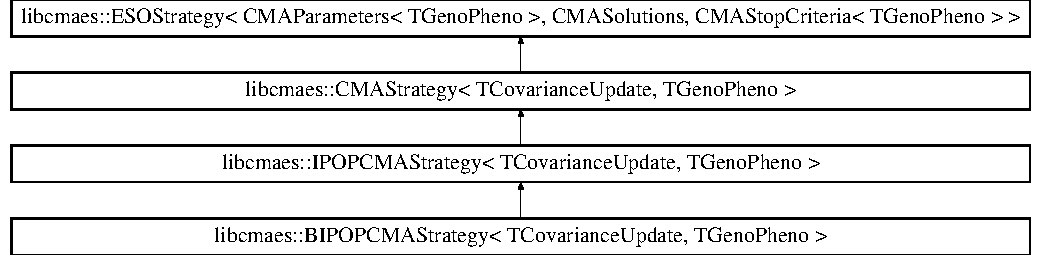
\includegraphics[height=3.430321cm]{classlibcmaes_1_1BIPOPCMAStrategy}
\end{center}
\end{figure}
\subsection*{Public Member Functions}
\begin{DoxyCompactItemize}
\item 
\hyperlink{classlibcmaes_1_1BIPOPCMAStrategy_a4c693467ab661f639e2fe2120dabcc6e}{B\+I\+P\+O\+P\+C\+M\+A\+Strategy} (Fit\+Func \&func, \hyperlink{classlibcmaes_1_1CMAParameters}{C\+M\+A\+Parameters}$<$ T\+Geno\+Pheno $>$ \&parameters)
\begin{DoxyCompactList}\small\item\em constructor. \end{DoxyCompactList}\item 
\hyperlink{classlibcmaes_1_1BIPOPCMAStrategy_a33ea94936c2a70c54d4b2e48f04f803f}{B\+I\+P\+O\+P\+C\+M\+A\+Strategy} (Fit\+Func \&func, \hyperlink{classlibcmaes_1_1CMAParameters}{C\+M\+A\+Parameters}$<$ T\+Geno\+Pheno $>$ \&parameters, const \hyperlink{classlibcmaes_1_1CMASolutions}{C\+M\+A\+Solutions} \&solutions)
\begin{DoxyCompactList}\small\item\em constructor. \end{DoxyCompactList}\item 
\hypertarget{classlibcmaes_1_1BIPOPCMAStrategy_adc3f5ef544a151efeb96e4d4c83e1858}{void \hyperlink{classlibcmaes_1_1BIPOPCMAStrategy_adc3f5ef544a151efeb96e4d4c83e1858}{tell} ()}\label{classlibcmaes_1_1BIPOPCMAStrategy_adc3f5ef544a151efeb96e4d4c83e1858}

\begin{DoxyCompactList}\small\item\em Updates the covariance matrix and prepares for the next iteration. \end{DoxyCompactList}\item 
int \hyperlink{classlibcmaes_1_1BIPOPCMAStrategy_a8646acea54a5e3775a040aa43fb6804c}{optimize} (const Eval\+Func \&evalf, const Ask\+Func \&askf, const Tell\+Func \&tellf)
\begin{DoxyCompactList}\small\item\em Finds the minimum of the objective function. It makes alternate calls to \hyperlink{classlibcmaes_1_1CMAStrategy_ab7266bc50732458ffcab690bc26380e6}{ask()}, \hyperlink{classlibcmaes_1_1BIPOPCMAStrategy_adc3f5ef544a151efeb96e4d4c83e1858}{tell()} and \hyperlink{classlibcmaes_1_1CMAStrategy_adc87b9c500959c800b6bc93d89432ecc}{stop()} until one of the termination criteria triggers. \end{DoxyCompactList}\item 
int \hyperlink{classlibcmaes_1_1BIPOPCMAStrategy_a7117a7300899d1b3b734ffc6efd41054}{optimize} ()
\begin{DoxyCompactList}\small\item\em Finds the minimum of the objective function. It makes alternate calls to \hyperlink{classlibcmaes_1_1CMAStrategy_ab7266bc50732458ffcab690bc26380e6}{ask()}, \hyperlink{classlibcmaes_1_1BIPOPCMAStrategy_adc3f5ef544a151efeb96e4d4c83e1858}{tell()} and \hyperlink{classlibcmaes_1_1CMAStrategy_adc87b9c500959c800b6bc93d89432ecc}{stop()} until one of the termination criteria triggers. \end{DoxyCompactList}\end{DoxyCompactItemize}
\subsection*{Protected Member Functions}
\begin{DoxyCompactItemize}
\item 
\hypertarget{classlibcmaes_1_1BIPOPCMAStrategy_a7285772ab91aa5da1bbb20485ed6136d}{void {\bfseries r1} ()}\label{classlibcmaes_1_1BIPOPCMAStrategy_a7285772ab91aa5da1bbb20485ed6136d}

\item 
\hypertarget{classlibcmaes_1_1BIPOPCMAStrategy_a1bf830b35350a9c9d63dd717dfab7c73}{void {\bfseries r2} ()}\label{classlibcmaes_1_1BIPOPCMAStrategy_a1bf830b35350a9c9d63dd717dfab7c73}

\end{DoxyCompactItemize}
\subsection*{Additional Inherited Members}


\subsection{Detailed Description}
\subsubsection*{template$<$class T\+Covariance\+Update, class T\+Geno\+Pheno$>$class libcmaes\+::\+B\+I\+P\+O\+P\+C\+M\+A\+Strategy$<$ T\+Covariance\+Update, T\+Geno\+Pheno $>$}

Implementation of the B\+I\+P\+O\+P flavor of C\+M\+A-\/\+E\+S, with restarts that control the population of offsprings used in the update of the distribution parameters in order to alternate between local and global searches for the objective. 

\subsection{Constructor \& Destructor Documentation}
\hypertarget{classlibcmaes_1_1BIPOPCMAStrategy_a4c693467ab661f639e2fe2120dabcc6e}{\index{libcmaes\+::\+B\+I\+P\+O\+P\+C\+M\+A\+Strategy@{libcmaes\+::\+B\+I\+P\+O\+P\+C\+M\+A\+Strategy}!B\+I\+P\+O\+P\+C\+M\+A\+Strategy@{B\+I\+P\+O\+P\+C\+M\+A\+Strategy}}
\index{B\+I\+P\+O\+P\+C\+M\+A\+Strategy@{B\+I\+P\+O\+P\+C\+M\+A\+Strategy}!libcmaes\+::\+B\+I\+P\+O\+P\+C\+M\+A\+Strategy@{libcmaes\+::\+B\+I\+P\+O\+P\+C\+M\+A\+Strategy}}
\subsubsection[{B\+I\+P\+O\+P\+C\+M\+A\+Strategy}]{\setlength{\rightskip}{0pt plus 5cm}template$<$class T\+Covariance\+Update , class T\+Geno\+Pheno $>$ {\bf libcmaes\+::\+B\+I\+P\+O\+P\+C\+M\+A\+Strategy}$<$ T\+Covariance\+Update, T\+Geno\+Pheno $>$\+::{\bf B\+I\+P\+O\+P\+C\+M\+A\+Strategy} (
\begin{DoxyParamCaption}
\item[{Fit\+Func \&}]{func, }
\item[{{\bf C\+M\+A\+Parameters}$<$ T\+Geno\+Pheno $>$ \&}]{parameters}
\end{DoxyParamCaption}
)}}\label{classlibcmaes_1_1BIPOPCMAStrategy_a4c693467ab661f639e2fe2120dabcc6e}


constructor. 


\begin{DoxyParams}{Parameters}
{\em func} & objective function to minimize \\
\hline
{\em parameters} & stochastic search parameters \\
\hline
\end{DoxyParams}
\hypertarget{classlibcmaes_1_1BIPOPCMAStrategy_a33ea94936c2a70c54d4b2e48f04f803f}{\index{libcmaes\+::\+B\+I\+P\+O\+P\+C\+M\+A\+Strategy@{libcmaes\+::\+B\+I\+P\+O\+P\+C\+M\+A\+Strategy}!B\+I\+P\+O\+P\+C\+M\+A\+Strategy@{B\+I\+P\+O\+P\+C\+M\+A\+Strategy}}
\index{B\+I\+P\+O\+P\+C\+M\+A\+Strategy@{B\+I\+P\+O\+P\+C\+M\+A\+Strategy}!libcmaes\+::\+B\+I\+P\+O\+P\+C\+M\+A\+Strategy@{libcmaes\+::\+B\+I\+P\+O\+P\+C\+M\+A\+Strategy}}
\subsubsection[{B\+I\+P\+O\+P\+C\+M\+A\+Strategy}]{\setlength{\rightskip}{0pt plus 5cm}template$<$class T\+Covariance\+Update , class T\+Geno\+Pheno $>$ {\bf libcmaes\+::\+B\+I\+P\+O\+P\+C\+M\+A\+Strategy}$<$ T\+Covariance\+Update, T\+Geno\+Pheno $>$\+::{\bf B\+I\+P\+O\+P\+C\+M\+A\+Strategy} (
\begin{DoxyParamCaption}
\item[{Fit\+Func \&}]{func, }
\item[{{\bf C\+M\+A\+Parameters}$<$ T\+Geno\+Pheno $>$ \&}]{parameters, }
\item[{const {\bf C\+M\+A\+Solutions} \&}]{solutions}
\end{DoxyParamCaption}
)}}\label{classlibcmaes_1_1BIPOPCMAStrategy_a33ea94936c2a70c54d4b2e48f04f803f}


constructor. 


\begin{DoxyParams}{Parameters}
{\em func} & objective function to minimize \\
\hline
{\em parameters} & stochastic search parameters \\
\hline
{\em solutions} & solution to start search from \\
\hline
\end{DoxyParams}


\subsection{Member Function Documentation}
\hypertarget{classlibcmaes_1_1BIPOPCMAStrategy_a8646acea54a5e3775a040aa43fb6804c}{\index{libcmaes\+::\+B\+I\+P\+O\+P\+C\+M\+A\+Strategy@{libcmaes\+::\+B\+I\+P\+O\+P\+C\+M\+A\+Strategy}!optimize@{optimize}}
\index{optimize@{optimize}!libcmaes\+::\+B\+I\+P\+O\+P\+C\+M\+A\+Strategy@{libcmaes\+::\+B\+I\+P\+O\+P\+C\+M\+A\+Strategy}}
\subsubsection[{optimize}]{\setlength{\rightskip}{0pt plus 5cm}template$<$class T\+Covariance\+Update , class T\+Geno\+Pheno $>$ int {\bf libcmaes\+::\+B\+I\+P\+O\+P\+C\+M\+A\+Strategy}$<$ T\+Covariance\+Update, T\+Geno\+Pheno $>$\+::optimize (
\begin{DoxyParamCaption}
\item[{const Eval\+Func \&}]{evalf, }
\item[{const Ask\+Func \&}]{askf, }
\item[{const Tell\+Func \&}]{tellf}
\end{DoxyParamCaption}
)}}\label{classlibcmaes_1_1BIPOPCMAStrategy_a8646acea54a5e3775a040aa43fb6804c}


Finds the minimum of the objective function. It makes alternate calls to \hyperlink{classlibcmaes_1_1CMAStrategy_ab7266bc50732458ffcab690bc26380e6}{ask()}, \hyperlink{classlibcmaes_1_1BIPOPCMAStrategy_adc3f5ef544a151efeb96e4d4c83e1858}{tell()} and \hyperlink{classlibcmaes_1_1CMAStrategy_adc87b9c500959c800b6bc93d89432ecc}{stop()} until one of the termination criteria triggers. 

\begin{DoxyReturn}{Returns}
success or error code, as defined in \hyperlink{opti__err_8h_source}{opti\+\_\+err.\+h} Note\+: the termination criteria code is held by \+\_\+solutions.\+\_\+run\+\_\+status 
\end{DoxyReturn}
\hypertarget{classlibcmaes_1_1BIPOPCMAStrategy_a7117a7300899d1b3b734ffc6efd41054}{\index{libcmaes\+::\+B\+I\+P\+O\+P\+C\+M\+A\+Strategy@{libcmaes\+::\+B\+I\+P\+O\+P\+C\+M\+A\+Strategy}!optimize@{optimize}}
\index{optimize@{optimize}!libcmaes\+::\+B\+I\+P\+O\+P\+C\+M\+A\+Strategy@{libcmaes\+::\+B\+I\+P\+O\+P\+C\+M\+A\+Strategy}}
\subsubsection[{optimize}]{\setlength{\rightskip}{0pt plus 5cm}template$<$class T\+Covariance\+Update , class T\+Geno\+Pheno $>$ int {\bf libcmaes\+::\+B\+I\+P\+O\+P\+C\+M\+A\+Strategy}$<$ T\+Covariance\+Update, T\+Geno\+Pheno $>$\+::optimize (
\begin{DoxyParamCaption}
{}
\end{DoxyParamCaption}
)\hspace{0.3cm}{\ttfamily [inline]}}}\label{classlibcmaes_1_1BIPOPCMAStrategy_a7117a7300899d1b3b734ffc6efd41054}


Finds the minimum of the objective function. It makes alternate calls to \hyperlink{classlibcmaes_1_1CMAStrategy_ab7266bc50732458ffcab690bc26380e6}{ask()}, \hyperlink{classlibcmaes_1_1BIPOPCMAStrategy_adc3f5ef544a151efeb96e4d4c83e1858}{tell()} and \hyperlink{classlibcmaes_1_1CMAStrategy_adc87b9c500959c800b6bc93d89432ecc}{stop()} until one of the termination criteria triggers. 


\begin{DoxyParams}{Parameters}
{\em evalf} & custom eval function \\
\hline
{\em askf} & custom ask function \\
\hline
{\em tellf} & custom tell function \\
\hline
\end{DoxyParams}
\begin{DoxyReturn}{Returns}
success or error code, as defined in \hyperlink{opti__err_8h_source}{opti\+\_\+err.\+h} Note\+: the termination criteria code is held by \+\_\+solutions.\+\_\+run\+\_\+status 
\end{DoxyReturn}


The documentation for this class was generated from the following files\+:\begin{DoxyCompactItemize}
\item 
src/bipopcmastrategy.\+h\item 
src/bipopcmastrategy.\+cc\end{DoxyCompactItemize}

\hypertarget{classlibcmaes_1_1Candidate}{\section{libcmaes\-:\-:Candidate Class Reference}
\label{classlibcmaes_1_1Candidate}\index{libcmaes\-::\-Candidate@{libcmaes\-::\-Candidate}}
}


candidate solution point, in function parameter space.  




{\ttfamily \#include $<$candidate.\-h$>$}

\subsection*{Public Member Functions}
\begin{DoxyCompactItemize}
\item 
\hypertarget{classlibcmaes_1_1Candidate_a40fca2abb2e1bcec470a79fa5ae6525f}{\hyperlink{classlibcmaes_1_1Candidate_a40fca2abb2e1bcec470a79fa5ae6525f}{Candidate} ()}\label{classlibcmaes_1_1Candidate_a40fca2abb2e1bcec470a79fa5ae6525f}

\begin{DoxyCompactList}\small\item\em empty constructor. \end{DoxyCompactList}\item 
\hyperlink{classlibcmaes_1_1Candidate_aa15c585a460bcc7e0537b8f8defea205}{Candidate} (const double \&fvalue, const d\-Vec \&x)
\begin{DoxyCompactList}\small\item\em constructor. \end{DoxyCompactList}\item 
\hypertarget{classlibcmaes_1_1Candidate_aeca2ab3de5182036093745ec7f82834d}{double {\bfseries get\-\_\-fvalue} () const }\label{classlibcmaes_1_1Candidate_aeca2ab3de5182036093745ec7f82834d}

\item 
\hypertarget{classlibcmaes_1_1Candidate_a6155af392159bfc4d10722a7a0abf420}{d\-Vec {\bfseries get\-\_\-x\-\_\-dvec} () const }\label{classlibcmaes_1_1Candidate_a6155af392159bfc4d10722a7a0abf420}

\item 
\hypertarget{classlibcmaes_1_1Candidate_a22455c702f36ca4ea8c389477f8a7d1e}{const double $\ast$ {\bfseries get\-\_\-x} () const }\label{classlibcmaes_1_1Candidate_a22455c702f36ca4ea8c389477f8a7d1e}

\item 
\hypertarget{classlibcmaes_1_1Candidate_a08ca200644dcfe1faab23dd933f10598}{{\footnotesize template$<$class T\-Geno\-Pheno $>$ }\\d\-Vec {\bfseries get\-\_\-x\-\_\-pheno} (const \hyperlink{classlibcmaes_1_1CMAParameters}{C\-M\-A\-Parameters}$<$ T\-Geno\-Pheno $>$ \&p) const }\label{classlibcmaes_1_1Candidate_a08ca200644dcfe1faab23dd933f10598}

\end{DoxyCompactItemize}
\subsection*{Public Attributes}
\begin{DoxyCompactItemize}
\item 
double \hyperlink{classlibcmaes_1_1Candidate_af8797627514ae7e137317337372fb67d}{\-\_\-fvalue}
\item 
d\-Vec \hyperlink{classlibcmaes_1_1Candidate_a0cded1d38ec7288e8064414c78023fe4}{\-\_\-x}
\end{DoxyCompactItemize}


\subsection{Detailed Description}
candidate solution point, in function parameter space. 

\subsection{Constructor \& Destructor Documentation}
\hypertarget{classlibcmaes_1_1Candidate_aa15c585a460bcc7e0537b8f8defea205}{\index{libcmaes\-::\-Candidate@{libcmaes\-::\-Candidate}!Candidate@{Candidate}}
\index{Candidate@{Candidate}!libcmaes::Candidate@{libcmaes\-::\-Candidate}}
\subsubsection[{Candidate}]{\setlength{\rightskip}{0pt plus 5cm}libcmaes\-::\-Candidate\-::\-Candidate (
\begin{DoxyParamCaption}
\item[{const double \&}]{fvalue, }
\item[{const d\-Vec \&}]{x}
\end{DoxyParamCaption}
)\hspace{0.3cm}{\ttfamily [inline]}}}\label{classlibcmaes_1_1Candidate_aa15c585a460bcc7e0537b8f8defea205}


constructor. 


\begin{DoxyParams}{Parameters}
{\em fvalue} & function value \\
\hline
{\em x} & function parameter vector \\
\hline
\end{DoxyParams}


\subsection{Member Data Documentation}
\hypertarget{classlibcmaes_1_1Candidate_af8797627514ae7e137317337372fb67d}{\index{libcmaes\-::\-Candidate@{libcmaes\-::\-Candidate}!\-\_\-fvalue@{\-\_\-fvalue}}
\index{\-\_\-fvalue@{\-\_\-fvalue}!libcmaes::Candidate@{libcmaes\-::\-Candidate}}
\subsubsection[{\-\_\-fvalue}]{\setlength{\rightskip}{0pt plus 5cm}double libcmaes\-::\-Candidate\-::\-\_\-fvalue}}\label{classlibcmaes_1_1Candidate_af8797627514ae7e137317337372fb67d}
function value. \hypertarget{classlibcmaes_1_1Candidate_a0cded1d38ec7288e8064414c78023fe4}{\index{libcmaes\-::\-Candidate@{libcmaes\-::\-Candidate}!\-\_\-x@{\-\_\-x}}
\index{\-\_\-x@{\-\_\-x}!libcmaes::Candidate@{libcmaes\-::\-Candidate}}
\subsubsection[{\-\_\-x}]{\setlength{\rightskip}{0pt plus 5cm}d\-Vec libcmaes\-::\-Candidate\-::\-\_\-x}}\label{classlibcmaes_1_1Candidate_a0cded1d38ec7288e8064414c78023fe4}
function parameter vector. 

The documentation for this class was generated from the following file\-:\begin{DoxyCompactItemize}
\item 
src/candidate.\-h\end{DoxyCompactItemize}

\hypertarget{classlibcmaes_1_1CMAParameters}{\section{libcmaes\-:\-:C\-M\-A\-Parameters$<$ T\-Geno\-Pheno $>$ Class Template Reference}
\label{classlibcmaes_1_1CMAParameters}\index{libcmaes\-::\-C\-M\-A\-Parameters$<$ T\-Geno\-Pheno $>$@{libcmaes\-::\-C\-M\-A\-Parameters$<$ T\-Geno\-Pheno $>$}}
}


\hyperlink{classlibcmaes_1_1Parameters}{Parameters} for various flavors of the C\-M\-A-\/\-E\-S algorithm.  




{\ttfamily \#include $<$cmaparameters.\-h$>$}

Inheritance diagram for libcmaes\-:\-:C\-M\-A\-Parameters$<$ T\-Geno\-Pheno $>$\-:\begin{figure}[H]
\begin{center}
\leavevmode
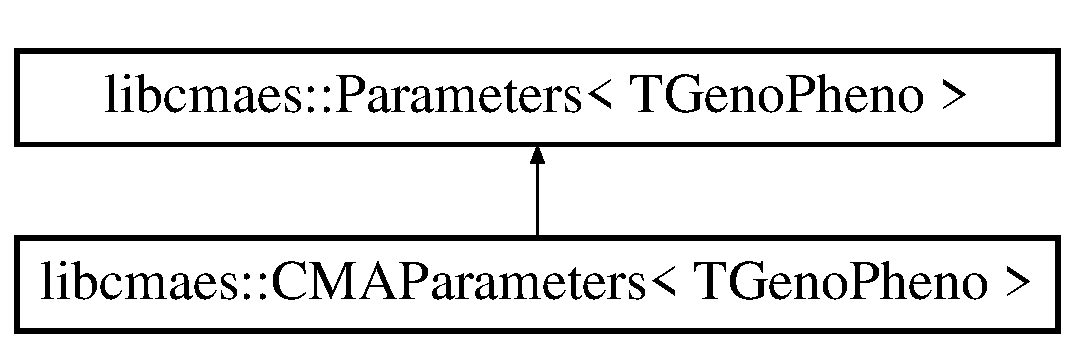
\includegraphics[height=2.000000cm]{classlibcmaes_1_1CMAParameters}
\end{center}
\end{figure}
\subsection*{Public Member Functions}
\begin{DoxyCompactItemize}
\item 
\hyperlink{classlibcmaes_1_1CMAParameters_a18d6039c0adffddd51caee1250b072bc}{C\-M\-A\-Parameters} (const int \&dim, const double $\ast$x0, const double \&sigma, const int \&lambda=-\/1, const uint64\-\_\-t \&seed=0, const T\-Geno\-Pheno \&gp=\hyperlink{classlibcmaes_1_1GenoPheno}{Geno\-Pheno}$<$ \hyperlink{classlibcmaes_1_1NoBoundStrategy}{No\-Bound\-Strategy} $>$())
\begin{DoxyCompactList}\small\item\em Constructor. \end{DoxyCompactList}\item 
\hypertarget{classlibcmaes_1_1CMAParameters_a0d963d4719d9b6447cddeeca542167a1}{void \hyperlink{classlibcmaes_1_1CMAParameters_a0d963d4719d9b6447cddeeca542167a1}{initialize\-\_\-parameters} ()}\label{classlibcmaes_1_1CMAParameters_a0d963d4719d9b6447cddeeca542167a1}

\begin{DoxyCompactList}\small\item\em initialize required parameters based on dim, lambda, x0 and sigma. \end{DoxyCompactList}\item 
\hypertarget{classlibcmaes_1_1CMAParameters_aa6dc1bafcff83e082db9146a923949d3}{void \hyperlink{classlibcmaes_1_1CMAParameters_aa6dc1bafcff83e082db9146a923949d3}{set\-\_\-noisy} ()}\label{classlibcmaes_1_1CMAParameters_aa6dc1bafcff83e082db9146a923949d3}

\begin{DoxyCompactList}\small\item\em adapt parameters for noisy objective function. \end{DoxyCompactList}\item 
\hypertarget{classlibcmaes_1_1CMAParameters_a1f2115c14728278a946c358d8d26f30c}{void \hyperlink{classlibcmaes_1_1CMAParameters_a1f2115c14728278a946c358d8d26f30c}{set\-\_\-sep} ()}\label{classlibcmaes_1_1CMAParameters_a1f2115c14728278a946c358d8d26f30c}

\begin{DoxyCompactList}\small\item\em fix parameters for sep-\/\-C\-M\-A-\/\-E\-S, using only the diagonal of covariance matrix. \end{DoxyCompactList}\item 
void \hyperlink{classlibcmaes_1_1CMAParameters_a7fcd592c259dca6716fdbe735fd1b837}{set\-\_\-automaxiter} (const bool \&b)
\begin{DoxyCompactList}\small\item\em turns stopping criteria Max\-Iter that automatically stops optimization after a number of steps on or off. \end{DoxyCompactList}\item 
void \hyperlink{classlibcmaes_1_1CMAParameters_a73af8cdc07dc3388c40a27ddbdea96b4}{set\-\_\-fixed\-\_\-p} (const int \&index, const double \&value)
\begin{DoxyCompactList}\small\item\em freezes a parameter to a given value during optimization. Adapts some generic parameters as well. \end{DoxyCompactList}\item 
void \hyperlink{classlibcmaes_1_1CMAParameters_a105789bdd00467411107db57302028f2}{set\-\_\-restarts} (const int \&nrestarts)
\begin{DoxyCompactList}\small\item\em sets the maximum number of restarts (applies to I\-P\-O\-P and B\-I\-P\-O\-P). \end{DoxyCompactList}\end{DoxyCompactItemize}
\subsection*{Public Attributes}
\begin{DoxyCompactItemize}
\item 
int \hyperlink{classlibcmaes_1_1CMAParameters_a102a49af5856035c4568178f4847e2e8}{\-\_\-mu}
\item 
d\-Vec \hyperlink{classlibcmaes_1_1CMAParameters_aa8eeb4ea2a91da73f1d53fa74d950049}{\-\_\-weights}
\item 
double \hyperlink{classlibcmaes_1_1CMAParameters_a9fc0879daeaeeb882192feddb0efecfc}{\-\_\-csigma}
\item 
double \hyperlink{classlibcmaes_1_1CMAParameters_ad6c921f865fc7fc344e8e1408baca772}{\-\_\-c1}
\item 
double \hyperlink{classlibcmaes_1_1CMAParameters_a0d4da3faa7fba9eb555d7dbfee7a6402}{\-\_\-cmu}
\item 
double \hyperlink{classlibcmaes_1_1CMAParameters_af85bfd2cef329712654fc697f50d5b4a}{\-\_\-cc}
\item 
double \hyperlink{classlibcmaes_1_1CMAParameters_afc24dfb50427ae6963515f8508f5759d}{\-\_\-muw}
\item 
double \hyperlink{classlibcmaes_1_1CMAParameters_a87f2b165fab84e65672361e5d6ac7f3d}{\-\_\-dsigma}
\item 
\hypertarget{classlibcmaes_1_1CMAParameters_abe4513aa9d69895e267c0ecde3bf5508}{double {\bfseries \-\_\-fact\-\_\-ps}}\label{classlibcmaes_1_1CMAParameters_abe4513aa9d69895e267c0ecde3bf5508}

\item 
\hypertarget{classlibcmaes_1_1CMAParameters_a24700ad95612d4a5d926b832ae02bcdf}{double {\bfseries \-\_\-fact\-\_\-pc}}\label{classlibcmaes_1_1CMAParameters_a24700ad95612d4a5d926b832ae02bcdf}

\item 
double \hyperlink{classlibcmaes_1_1CMAParameters_ab63f8f5d707242ec981945df88a573db}{\-\_\-chi}
\item 
double \hyperlink{classlibcmaes_1_1CMAParameters_a8ad9eb52bd8ffcfc4ea175fef21c8f96}{\-\_\-sigma\-\_\-init}
\item 
int \hyperlink{classlibcmaes_1_1CMAParameters_a2ccf2865600fe20d965af9bdf9c6ab60}{\-\_\-nrestarts} = 9
\item 
bool \hyperlink{classlibcmaes_1_1CMAParameters_ac65bf2bb1b20461cfe8bd58175727ccc}{\-\_\-lazy\-\_\-update}
\item 
double \hyperlink{classlibcmaes_1_1CMAParameters_ae00e6b49bd99e1aa316bec03da96e95b}{\-\_\-lazy\-\_\-value}
\item 
double \hyperlink{classlibcmaes_1_1CMAParameters_a34e3414332daf15d81b353c7de803e1d}{\-\_\-cm}
\item 
double \hyperlink{classlibcmaes_1_1CMAParameters_ae13b411e5035c574e1521afa4b6d734b}{\-\_\-alphacov}
\item 
double \hyperlink{classlibcmaes_1_1CMAParameters_a3dfb7a180cb3746a4bc3a2d82b8a8f35}{\-\_\-alphaminusold}
\item 
double \hyperlink{classlibcmaes_1_1CMAParameters_a011a9f790bc21c6bea155066a26f5181}{\-\_\-deltamaxsigma}
\item 
double \hyperlink{classlibcmaes_1_1CMAParameters_afc8800d362e2b25074610b883684156b}{\-\_\-lambdamintarget}
\item 
double \hyperlink{classlibcmaes_1_1CMAParameters_a8d4e4afdbdb72635241846562fc37a04}{\-\_\-alphaminusmin}
\item 
bool \hyperlink{classlibcmaes_1_1CMAParameters_ad7f26f864149ce4d62169e15daa530fa}{\-\_\-sep} = false
\item 
bool \hyperlink{classlibcmaes_1_1CMAParameters_a9a66e6d8cf1e1c67cd9c43d5c87a71d1}{\-\_\-has\-\_\-max\-\_\-iter} = true
\end{DoxyCompactItemize}


\subsection{Detailed Description}
\subsubsection*{template$<$class T\-Geno\-Pheno = Geno\-Pheno$<$\-No\-Bound\-Strategy$>$$>$class libcmaes\-::\-C\-M\-A\-Parameters$<$ T\-Geno\-Pheno $>$}

\hyperlink{classlibcmaes_1_1Parameters}{Parameters} for various flavors of the C\-M\-A-\/\-E\-S algorithm. 

\subsection{Constructor \& Destructor Documentation}
\hypertarget{classlibcmaes_1_1CMAParameters_a18d6039c0adffddd51caee1250b072bc}{\index{libcmaes\-::\-C\-M\-A\-Parameters@{libcmaes\-::\-C\-M\-A\-Parameters}!C\-M\-A\-Parameters@{C\-M\-A\-Parameters}}
\index{C\-M\-A\-Parameters@{C\-M\-A\-Parameters}!libcmaes::CMAParameters@{libcmaes\-::\-C\-M\-A\-Parameters}}
\subsubsection[{C\-M\-A\-Parameters}]{\setlength{\rightskip}{0pt plus 5cm}template$<$class T\-Geno\-Pheno$>$ {\bf libcmaes\-::\-C\-M\-A\-Parameters}$<$ T\-Geno\-Pheno $>$\-::{\bf C\-M\-A\-Parameters} (
\begin{DoxyParamCaption}
\item[{const int \&}]{dim, }
\item[{const double $\ast$}]{x0, }
\item[{const double \&}]{sigma, }
\item[{const int \&}]{lambda = {\ttfamily -\/1}, }
\item[{const uint64\-\_\-t \&}]{seed = {\ttfamily 0}, }
\item[{const T\-Geno\-Pheno \&}]{gp = {\ttfamily {\bf Geno\-Pheno}$<${\bf No\-Bound\-Strategy}$>$()}}
\end{DoxyParamCaption}
)}}\label{classlibcmaes_1_1CMAParameters_a18d6039c0adffddd51caee1250b072bc}


Constructor. 


\begin{DoxyParams}{Parameters}
{\em dim} & problem dimensions \\
\hline
{\em x0} & initial search point \\
\hline
{\em sigma} & initial distribution step size (positive, otherwise automatically set) \\
\hline
{\em lambda} & number of offsprings sampled at each step \\
\hline
{\em seed} & initial random seed, useful for reproducing results (if unspecified, automatically generated from current time) \\
\hline
{\em gp} & genotype / phenotype object \\
\hline
{\em sep} & whether to use sep-\/\-C\-M\-A-\/\-E\-S, using diagonal covariance matrix (modifies covariance default learning rate) \\
\hline
\end{DoxyParams}


\subsection{Member Function Documentation}
\hypertarget{classlibcmaes_1_1CMAParameters_a7fcd592c259dca6716fdbe735fd1b837}{\index{libcmaes\-::\-C\-M\-A\-Parameters@{libcmaes\-::\-C\-M\-A\-Parameters}!set\-\_\-automaxiter@{set\-\_\-automaxiter}}
\index{set\-\_\-automaxiter@{set\-\_\-automaxiter}!libcmaes::CMAParameters@{libcmaes\-::\-C\-M\-A\-Parameters}}
\subsubsection[{set\-\_\-automaxiter}]{\setlength{\rightskip}{0pt plus 5cm}template$<$class T\-Geno\-Pheno = Geno\-Pheno$<$\-No\-Bound\-Strategy$>$$>$ void {\bf libcmaes\-::\-C\-M\-A\-Parameters}$<$ T\-Geno\-Pheno $>$\-::set\-\_\-automaxiter (
\begin{DoxyParamCaption}
\item[{const bool \&}]{b}
\end{DoxyParamCaption}
)\hspace{0.3cm}{\ttfamily [inline]}}}\label{classlibcmaes_1_1CMAParameters_a7fcd592c259dca6716fdbe735fd1b837}


turns stopping criteria Max\-Iter that automatically stops optimization after a number of steps on or off. 


\begin{DoxyParams}{Parameters}
{\em b} & true or false for turning criteria on or off (on is default in constructor). \\
\hline
\end{DoxyParams}
\hypertarget{classlibcmaes_1_1CMAParameters_a73af8cdc07dc3388c40a27ddbdea96b4}{\index{libcmaes\-::\-C\-M\-A\-Parameters@{libcmaes\-::\-C\-M\-A\-Parameters}!set\-\_\-fixed\-\_\-p@{set\-\_\-fixed\-\_\-p}}
\index{set\-\_\-fixed\-\_\-p@{set\-\_\-fixed\-\_\-p}!libcmaes::CMAParameters@{libcmaes\-::\-C\-M\-A\-Parameters}}
\subsubsection[{set\-\_\-fixed\-\_\-p}]{\setlength{\rightskip}{0pt plus 5cm}template$<$class T\-Geno\-Pheno $>$ void {\bf libcmaes\-::\-C\-M\-A\-Parameters}$<$ T\-Geno\-Pheno $>$\-::set\-\_\-fixed\-\_\-p (
\begin{DoxyParamCaption}
\item[{const int \&}]{index, }
\item[{const double \&}]{value}
\end{DoxyParamCaption}
)}}\label{classlibcmaes_1_1CMAParameters_a73af8cdc07dc3388c40a27ddbdea96b4}


freezes a parameter to a given value during optimization. Adapts some generic parameters as well. 


\begin{DoxyParams}{Parameters}
{\em index} & dimension index of the parameter to be frozen \\
\hline
{\em value} & frozen value of the parameter \\
\hline
\end{DoxyParams}
\hypertarget{classlibcmaes_1_1CMAParameters_a105789bdd00467411107db57302028f2}{\index{libcmaes\-::\-C\-M\-A\-Parameters@{libcmaes\-::\-C\-M\-A\-Parameters}!set\-\_\-restarts@{set\-\_\-restarts}}
\index{set\-\_\-restarts@{set\-\_\-restarts}!libcmaes::CMAParameters@{libcmaes\-::\-C\-M\-A\-Parameters}}
\subsubsection[{set\-\_\-restarts}]{\setlength{\rightskip}{0pt plus 5cm}template$<$class T\-Geno\-Pheno = Geno\-Pheno$<$\-No\-Bound\-Strategy$>$$>$ void {\bf libcmaes\-::\-C\-M\-A\-Parameters}$<$ T\-Geno\-Pheno $>$\-::set\-\_\-restarts (
\begin{DoxyParamCaption}
\item[{const int \&}]{nrestarts}
\end{DoxyParamCaption}
)\hspace{0.3cm}{\ttfamily [inline]}}}\label{classlibcmaes_1_1CMAParameters_a105789bdd00467411107db57302028f2}


sets the maximum number of restarts (applies to I\-P\-O\-P and B\-I\-P\-O\-P). 


\begin{DoxyParams}{Parameters}
{\em nrestarts} & maximum number of restarts \\
\hline
\end{DoxyParams}


\subsection{Member Data Documentation}
\hypertarget{classlibcmaes_1_1CMAParameters_ae13b411e5035c574e1521afa4b6d734b}{\index{libcmaes\-::\-C\-M\-A\-Parameters@{libcmaes\-::\-C\-M\-A\-Parameters}!\-\_\-alphacov@{\-\_\-alphacov}}
\index{\-\_\-alphacov@{\-\_\-alphacov}!libcmaes::CMAParameters@{libcmaes\-::\-C\-M\-A\-Parameters}}
\subsubsection[{\-\_\-alphacov}]{\setlength{\rightskip}{0pt plus 5cm}template$<$class T\-Geno\-Pheno = Geno\-Pheno$<$\-No\-Bound\-Strategy$>$$>$ double {\bf libcmaes\-::\-C\-M\-A\-Parameters}$<$ T\-Geno\-Pheno $>$\-::\-\_\-alphacov}}\label{classlibcmaes_1_1CMAParameters_ae13b411e5035c574e1521afa4b6d734b}
= 2 (active C\-M\-A only) \hypertarget{classlibcmaes_1_1CMAParameters_a8d4e4afdbdb72635241846562fc37a04}{\index{libcmaes\-::\-C\-M\-A\-Parameters@{libcmaes\-::\-C\-M\-A\-Parameters}!\-\_\-alphaminusmin@{\-\_\-alphaminusmin}}
\index{\-\_\-alphaminusmin@{\-\_\-alphaminusmin}!libcmaes::CMAParameters@{libcmaes\-::\-C\-M\-A\-Parameters}}
\subsubsection[{\-\_\-alphaminusmin}]{\setlength{\rightskip}{0pt plus 5cm}template$<$class T\-Geno\-Pheno = Geno\-Pheno$<$\-No\-Bound\-Strategy$>$$>$ double {\bf libcmaes\-::\-C\-M\-A\-Parameters}$<$ T\-Geno\-Pheno $>$\-::\-\_\-alphaminusmin}}\label{classlibcmaes_1_1CMAParameters_a8d4e4afdbdb72635241846562fc37a04}
= 1 (active C\-M\-A only) \hypertarget{classlibcmaes_1_1CMAParameters_a3dfb7a180cb3746a4bc3a2d82b8a8f35}{\index{libcmaes\-::\-C\-M\-A\-Parameters@{libcmaes\-::\-C\-M\-A\-Parameters}!\-\_\-alphaminusold@{\-\_\-alphaminusold}}
\index{\-\_\-alphaminusold@{\-\_\-alphaminusold}!libcmaes::CMAParameters@{libcmaes\-::\-C\-M\-A\-Parameters}}
\subsubsection[{\-\_\-alphaminusold}]{\setlength{\rightskip}{0pt plus 5cm}template$<$class T\-Geno\-Pheno = Geno\-Pheno$<$\-No\-Bound\-Strategy$>$$>$ double {\bf libcmaes\-::\-C\-M\-A\-Parameters}$<$ T\-Geno\-Pheno $>$\-::\-\_\-alphaminusold}}\label{classlibcmaes_1_1CMAParameters_a3dfb7a180cb3746a4bc3a2d82b8a8f35}
in \mbox{[}0,1\mbox{]} (active C\-M\-A only) \hypertarget{classlibcmaes_1_1CMAParameters_ad6c921f865fc7fc344e8e1408baca772}{\index{libcmaes\-::\-C\-M\-A\-Parameters@{libcmaes\-::\-C\-M\-A\-Parameters}!\-\_\-c1@{\-\_\-c1}}
\index{\-\_\-c1@{\-\_\-c1}!libcmaes::CMAParameters@{libcmaes\-::\-C\-M\-A\-Parameters}}
\subsubsection[{\-\_\-c1}]{\setlength{\rightskip}{0pt plus 5cm}template$<$class T\-Geno\-Pheno = Geno\-Pheno$<$\-No\-Bound\-Strategy$>$$>$ double {\bf libcmaes\-::\-C\-M\-A\-Parameters}$<$ T\-Geno\-Pheno $>$\-::\-\_\-c1}}\label{classlibcmaes_1_1CMAParameters_ad6c921f865fc7fc344e8e1408baca772}
covariance matrix learning rate for the rank one update using pc. \hypertarget{classlibcmaes_1_1CMAParameters_af85bfd2cef329712654fc697f50d5b4a}{\index{libcmaes\-::\-C\-M\-A\-Parameters@{libcmaes\-::\-C\-M\-A\-Parameters}!\-\_\-cc@{\-\_\-cc}}
\index{\-\_\-cc@{\-\_\-cc}!libcmaes::CMAParameters@{libcmaes\-::\-C\-M\-A\-Parameters}}
\subsubsection[{\-\_\-cc}]{\setlength{\rightskip}{0pt plus 5cm}template$<$class T\-Geno\-Pheno = Geno\-Pheno$<$\-No\-Bound\-Strategy$>$$>$ double {\bf libcmaes\-::\-C\-M\-A\-Parameters}$<$ T\-Geno\-Pheno $>$\-::\-\_\-cc}}\label{classlibcmaes_1_1CMAParameters_af85bfd2cef329712654fc697f50d5b4a}
cumulation constant for pc. \hypertarget{classlibcmaes_1_1CMAParameters_ab63f8f5d707242ec981945df88a573db}{\index{libcmaes\-::\-C\-M\-A\-Parameters@{libcmaes\-::\-C\-M\-A\-Parameters}!\-\_\-chi@{\-\_\-chi}}
\index{\-\_\-chi@{\-\_\-chi}!libcmaes::CMAParameters@{libcmaes\-::\-C\-M\-A\-Parameters}}
\subsubsection[{\-\_\-chi}]{\setlength{\rightskip}{0pt plus 5cm}template$<$class T\-Geno\-Pheno = Geno\-Pheno$<$\-No\-Bound\-Strategy$>$$>$ double {\bf libcmaes\-::\-C\-M\-A\-Parameters}$<$ T\-Geno\-Pheno $>$\-::\-\_\-chi}}\label{classlibcmaes_1_1CMAParameters_ab63f8f5d707242ec981945df88a573db}
norm of N(0,\-I) \hypertarget{classlibcmaes_1_1CMAParameters_a34e3414332daf15d81b353c7de803e1d}{\index{libcmaes\-::\-C\-M\-A\-Parameters@{libcmaes\-::\-C\-M\-A\-Parameters}!\-\_\-cm@{\-\_\-cm}}
\index{\-\_\-cm@{\-\_\-cm}!libcmaes::CMAParameters@{libcmaes\-::\-C\-M\-A\-Parameters}}
\subsubsection[{\-\_\-cm}]{\setlength{\rightskip}{0pt plus 5cm}template$<$class T\-Geno\-Pheno = Geno\-Pheno$<$\-No\-Bound\-Strategy$>$$>$ double {\bf libcmaes\-::\-C\-M\-A\-Parameters}$<$ T\-Geno\-Pheno $>$\-::\-\_\-cm}}\label{classlibcmaes_1_1CMAParameters_a34e3414332daf15d81b353c7de803e1d}
learning rate for the mean. \hypertarget{classlibcmaes_1_1CMAParameters_a0d4da3faa7fba9eb555d7dbfee7a6402}{\index{libcmaes\-::\-C\-M\-A\-Parameters@{libcmaes\-::\-C\-M\-A\-Parameters}!\-\_\-cmu@{\-\_\-cmu}}
\index{\-\_\-cmu@{\-\_\-cmu}!libcmaes::CMAParameters@{libcmaes\-::\-C\-M\-A\-Parameters}}
\subsubsection[{\-\_\-cmu}]{\setlength{\rightskip}{0pt plus 5cm}template$<$class T\-Geno\-Pheno = Geno\-Pheno$<$\-No\-Bound\-Strategy$>$$>$ double {\bf libcmaes\-::\-C\-M\-A\-Parameters}$<$ T\-Geno\-Pheno $>$\-::\-\_\-cmu}}\label{classlibcmaes_1_1CMAParameters_a0d4da3faa7fba9eb555d7dbfee7a6402}
covariance matrix learning reate for the rank mu update. \hypertarget{classlibcmaes_1_1CMAParameters_a9fc0879daeaeeb882192feddb0efecfc}{\index{libcmaes\-::\-C\-M\-A\-Parameters@{libcmaes\-::\-C\-M\-A\-Parameters}!\-\_\-csigma@{\-\_\-csigma}}
\index{\-\_\-csigma@{\-\_\-csigma}!libcmaes::CMAParameters@{libcmaes\-::\-C\-M\-A\-Parameters}}
\subsubsection[{\-\_\-csigma}]{\setlength{\rightskip}{0pt plus 5cm}template$<$class T\-Geno\-Pheno = Geno\-Pheno$<$\-No\-Bound\-Strategy$>$$>$ double {\bf libcmaes\-::\-C\-M\-A\-Parameters}$<$ T\-Geno\-Pheno $>$\-::\-\_\-csigma}}\label{classlibcmaes_1_1CMAParameters_a9fc0879daeaeeb882192feddb0efecfc}
cumulation constant for step size. \hypertarget{classlibcmaes_1_1CMAParameters_a011a9f790bc21c6bea155066a26f5181}{\index{libcmaes\-::\-C\-M\-A\-Parameters@{libcmaes\-::\-C\-M\-A\-Parameters}!\-\_\-deltamaxsigma@{\-\_\-deltamaxsigma}}
\index{\-\_\-deltamaxsigma@{\-\_\-deltamaxsigma}!libcmaes::CMAParameters@{libcmaes\-::\-C\-M\-A\-Parameters}}
\subsubsection[{\-\_\-deltamaxsigma}]{\setlength{\rightskip}{0pt plus 5cm}template$<$class T\-Geno\-Pheno = Geno\-Pheno$<$\-No\-Bound\-Strategy$>$$>$ double {\bf libcmaes\-::\-C\-M\-A\-Parameters}$<$ T\-Geno\-Pheno $>$\-::\-\_\-deltamaxsigma}}\label{classlibcmaes_1_1CMAParameters_a011a9f790bc21c6bea155066a26f5181}
infinite (active C\-M\-A only) \hypertarget{classlibcmaes_1_1CMAParameters_a87f2b165fab84e65672361e5d6ac7f3d}{\index{libcmaes\-::\-C\-M\-A\-Parameters@{libcmaes\-::\-C\-M\-A\-Parameters}!\-\_\-dsigma@{\-\_\-dsigma}}
\index{\-\_\-dsigma@{\-\_\-dsigma}!libcmaes::CMAParameters@{libcmaes\-::\-C\-M\-A\-Parameters}}
\subsubsection[{\-\_\-dsigma}]{\setlength{\rightskip}{0pt plus 5cm}template$<$class T\-Geno\-Pheno = Geno\-Pheno$<$\-No\-Bound\-Strategy$>$$>$ double {\bf libcmaes\-::\-C\-M\-A\-Parameters}$<$ T\-Geno\-Pheno $>$\-::\-\_\-dsigma}}\label{classlibcmaes_1_1CMAParameters_a87f2b165fab84e65672361e5d6ac7f3d}
step size damping factor. \hypertarget{classlibcmaes_1_1CMAParameters_a9a66e6d8cf1e1c67cd9c43d5c87a71d1}{\index{libcmaes\-::\-C\-M\-A\-Parameters@{libcmaes\-::\-C\-M\-A\-Parameters}!\-\_\-has\-\_\-max\-\_\-iter@{\-\_\-has\-\_\-max\-\_\-iter}}
\index{\-\_\-has\-\_\-max\-\_\-iter@{\-\_\-has\-\_\-max\-\_\-iter}!libcmaes::CMAParameters@{libcmaes\-::\-C\-M\-A\-Parameters}}
\subsubsection[{\-\_\-has\-\_\-max\-\_\-iter}]{\setlength{\rightskip}{0pt plus 5cm}template$<$class T\-Geno\-Pheno = Geno\-Pheno$<$\-No\-Bound\-Strategy$>$$>$ bool {\bf libcmaes\-::\-C\-M\-A\-Parameters}$<$ T\-Geno\-Pheno $>$\-::\-\_\-has\-\_\-max\-\_\-iter = true}}\label{classlibcmaes_1_1CMAParameters_a9a66e6d8cf1e1c67cd9c43d5c87a71d1}
Max\-Iter criteria\-: automatically stop running after 100+50$\ast$((D+2)$^\wedge$2)/lambda iterations. \hypertarget{classlibcmaes_1_1CMAParameters_afc8800d362e2b25074610b883684156b}{\index{libcmaes\-::\-C\-M\-A\-Parameters@{libcmaes\-::\-C\-M\-A\-Parameters}!\-\_\-lambdamintarget@{\-\_\-lambdamintarget}}
\index{\-\_\-lambdamintarget@{\-\_\-lambdamintarget}!libcmaes::CMAParameters@{libcmaes\-::\-C\-M\-A\-Parameters}}
\subsubsection[{\-\_\-lambdamintarget}]{\setlength{\rightskip}{0pt plus 5cm}template$<$class T\-Geno\-Pheno = Geno\-Pheno$<$\-No\-Bound\-Strategy$>$$>$ double {\bf libcmaes\-::\-C\-M\-A\-Parameters}$<$ T\-Geno\-Pheno $>$\-::\-\_\-lambdamintarget}}\label{classlibcmaes_1_1CMAParameters_afc8800d362e2b25074610b883684156b}
= 0.\-66 (active C\-M\-A only) \hypertarget{classlibcmaes_1_1CMAParameters_ac65bf2bb1b20461cfe8bd58175727ccc}{\index{libcmaes\-::\-C\-M\-A\-Parameters@{libcmaes\-::\-C\-M\-A\-Parameters}!\-\_\-lazy\-\_\-update@{\-\_\-lazy\-\_\-update}}
\index{\-\_\-lazy\-\_\-update@{\-\_\-lazy\-\_\-update}!libcmaes::CMAParameters@{libcmaes\-::\-C\-M\-A\-Parameters}}
\subsubsection[{\-\_\-lazy\-\_\-update}]{\setlength{\rightskip}{0pt plus 5cm}template$<$class T\-Geno\-Pheno = Geno\-Pheno$<$\-No\-Bound\-Strategy$>$$>$ bool {\bf libcmaes\-::\-C\-M\-A\-Parameters}$<$ T\-Geno\-Pheno $>$\-::\-\_\-lazy\-\_\-update}}\label{classlibcmaes_1_1CMAParameters_ac65bf2bb1b20461cfe8bd58175727ccc}
covariance lazy update. \hypertarget{classlibcmaes_1_1CMAParameters_ae00e6b49bd99e1aa316bec03da96e95b}{\index{libcmaes\-::\-C\-M\-A\-Parameters@{libcmaes\-::\-C\-M\-A\-Parameters}!\-\_\-lazy\-\_\-value@{\-\_\-lazy\-\_\-value}}
\index{\-\_\-lazy\-\_\-value@{\-\_\-lazy\-\_\-value}!libcmaes::CMAParameters@{libcmaes\-::\-C\-M\-A\-Parameters}}
\subsubsection[{\-\_\-lazy\-\_\-value}]{\setlength{\rightskip}{0pt plus 5cm}template$<$class T\-Geno\-Pheno = Geno\-Pheno$<$\-No\-Bound\-Strategy$>$$>$ double {\bf libcmaes\-::\-C\-M\-A\-Parameters}$<$ T\-Geno\-Pheno $>$\-::\-\_\-lazy\-\_\-value}}\label{classlibcmaes_1_1CMAParameters_ae00e6b49bd99e1aa316bec03da96e95b}
reference trigger for lazy update. \hypertarget{classlibcmaes_1_1CMAParameters_a102a49af5856035c4568178f4847e2e8}{\index{libcmaes\-::\-C\-M\-A\-Parameters@{libcmaes\-::\-C\-M\-A\-Parameters}!\-\_\-mu@{\-\_\-mu}}
\index{\-\_\-mu@{\-\_\-mu}!libcmaes::CMAParameters@{libcmaes\-::\-C\-M\-A\-Parameters}}
\subsubsection[{\-\_\-mu}]{\setlength{\rightskip}{0pt plus 5cm}template$<$class T\-Geno\-Pheno = Geno\-Pheno$<$\-No\-Bound\-Strategy$>$$>$ int {\bf libcmaes\-::\-C\-M\-A\-Parameters}$<$ T\-Geno\-Pheno $>$\-::\-\_\-mu}}\label{classlibcmaes_1_1CMAParameters_a102a49af5856035c4568178f4847e2e8}
number of candidate solutions used to update the distribution parameters. \hypertarget{classlibcmaes_1_1CMAParameters_afc24dfb50427ae6963515f8508f5759d}{\index{libcmaes\-::\-C\-M\-A\-Parameters@{libcmaes\-::\-C\-M\-A\-Parameters}!\-\_\-muw@{\-\_\-muw}}
\index{\-\_\-muw@{\-\_\-muw}!libcmaes::CMAParameters@{libcmaes\-::\-C\-M\-A\-Parameters}}
\subsubsection[{\-\_\-muw}]{\setlength{\rightskip}{0pt plus 5cm}template$<$class T\-Geno\-Pheno = Geno\-Pheno$<$\-No\-Bound\-Strategy$>$$>$ double {\bf libcmaes\-::\-C\-M\-A\-Parameters}$<$ T\-Geno\-Pheno $>$\-::\-\_\-muw}}\label{classlibcmaes_1_1CMAParameters_afc24dfb50427ae6963515f8508f5759d}
$^\wedge$ \-\_\-weights . \hypertarget{classlibcmaes_1_1CMAParameters_a2ccf2865600fe20d965af9bdf9c6ab60}{\index{libcmaes\-::\-C\-M\-A\-Parameters@{libcmaes\-::\-C\-M\-A\-Parameters}!\-\_\-nrestarts@{\-\_\-nrestarts}}
\index{\-\_\-nrestarts@{\-\_\-nrestarts}!libcmaes::CMAParameters@{libcmaes\-::\-C\-M\-A\-Parameters}}
\subsubsection[{\-\_\-nrestarts}]{\setlength{\rightskip}{0pt plus 5cm}template$<$class T\-Geno\-Pheno = Geno\-Pheno$<$\-No\-Bound\-Strategy$>$$>$ int {\bf libcmaes\-::\-C\-M\-A\-Parameters}$<$ T\-Geno\-Pheno $>$\-::\-\_\-nrestarts = 9}}\label{classlibcmaes_1_1CMAParameters_a2ccf2865600fe20d965af9bdf9c6ab60}
maximum number of restart, when applicable. \hypertarget{classlibcmaes_1_1CMAParameters_ad7f26f864149ce4d62169e15daa530fa}{\index{libcmaes\-::\-C\-M\-A\-Parameters@{libcmaes\-::\-C\-M\-A\-Parameters}!\-\_\-sep@{\-\_\-sep}}
\index{\-\_\-sep@{\-\_\-sep}!libcmaes::CMAParameters@{libcmaes\-::\-C\-M\-A\-Parameters}}
\subsubsection[{\-\_\-sep}]{\setlength{\rightskip}{0pt plus 5cm}template$<$class T\-Geno\-Pheno = Geno\-Pheno$<$\-No\-Bound\-Strategy$>$$>$ bool {\bf libcmaes\-::\-C\-M\-A\-Parameters}$<$ T\-Geno\-Pheno $>$\-::\-\_\-sep = false}}\label{classlibcmaes_1_1CMAParameters_ad7f26f864149ce4d62169e15daa530fa}
whether to use diagonal covariance matrix. \hypertarget{classlibcmaes_1_1CMAParameters_a8ad9eb52bd8ffcfc4ea175fef21c8f96}{\index{libcmaes\-::\-C\-M\-A\-Parameters@{libcmaes\-::\-C\-M\-A\-Parameters}!\-\_\-sigma\-\_\-init@{\-\_\-sigma\-\_\-init}}
\index{\-\_\-sigma\-\_\-init@{\-\_\-sigma\-\_\-init}!libcmaes::CMAParameters@{libcmaes\-::\-C\-M\-A\-Parameters}}
\subsubsection[{\-\_\-sigma\-\_\-init}]{\setlength{\rightskip}{0pt plus 5cm}template$<$class T\-Geno\-Pheno = Geno\-Pheno$<$\-No\-Bound\-Strategy$>$$>$ double {\bf libcmaes\-::\-C\-M\-A\-Parameters}$<$ T\-Geno\-Pheno $>$\-::\-\_\-sigma\-\_\-init}}\label{classlibcmaes_1_1CMAParameters_a8ad9eb52bd8ffcfc4ea175fef21c8f96}
initial sigma value. \hypertarget{classlibcmaes_1_1CMAParameters_aa8eeb4ea2a91da73f1d53fa74d950049}{\index{libcmaes\-::\-C\-M\-A\-Parameters@{libcmaes\-::\-C\-M\-A\-Parameters}!\-\_\-weights@{\-\_\-weights}}
\index{\-\_\-weights@{\-\_\-weights}!libcmaes::CMAParameters@{libcmaes\-::\-C\-M\-A\-Parameters}}
\subsubsection[{\-\_\-weights}]{\setlength{\rightskip}{0pt plus 5cm}template$<$class T\-Geno\-Pheno = Geno\-Pheno$<$\-No\-Bound\-Strategy$>$$>$ d\-Vec {\bf libcmaes\-::\-C\-M\-A\-Parameters}$<$ T\-Geno\-Pheno $>$\-::\-\_\-weights}}\label{classlibcmaes_1_1CMAParameters_aa8eeb4ea2a91da73f1d53fa74d950049}
offsprings weighting scheme. 

The documentation for this class was generated from the following files\-:\begin{DoxyCompactItemize}
\item 
src/cmaparameters.\-h\item 
src/cmaparameters.\-cc\end{DoxyCompactItemize}

\hypertarget{classlibcmaes_1_1CMASolutions}{\section{libcmaes\+:\+:C\+M\+A\+Solutions Class Reference}
\label{classlibcmaes_1_1CMASolutions}\index{libcmaes\+::\+C\+M\+A\+Solutions@{libcmaes\+::\+C\+M\+A\+Solutions}}
}


Holder of the set of evolving solutions from running an instance of C\+M\+A-\/\+E\+S.  




{\ttfamily \#include $<$cmasolutions.\+h$>$}

\subsection*{Public Member Functions}
\begin{DoxyCompactItemize}
\item 
\hypertarget{classlibcmaes_1_1CMASolutions_adc7194ca66777833c1980d11bc79649b}{\hyperlink{classlibcmaes_1_1CMASolutions_adc7194ca66777833c1980d11bc79649b}{C\+M\+A\+Solutions} ()}\label{classlibcmaes_1_1CMASolutions_adc7194ca66777833c1980d11bc79649b}

\begin{DoxyCompactList}\small\item\em dummy constructor. \end{DoxyCompactList}\item 
{\footnotesize template$<$class T\+Geno\+Pheno  = Geno\+Pheno$<$\+No\+Bound\+Strategy$>$$>$ }\\\hyperlink{classlibcmaes_1_1CMASolutions_acb424e8b0329ee8790be4156aef68c4f}{C\+M\+A\+Solutions} (\hyperlink{classlibcmaes_1_1Parameters}{Parameters}$<$ T\+Geno\+Pheno $>$ \&p)
\begin{DoxyCompactList}\small\item\em initializes solutions from stochastic optimization parameters. \end{DoxyCompactList}\item 
\hypertarget{classlibcmaes_1_1CMASolutions_a48934296b4295080786cbc97302448f7}{void \hyperlink{classlibcmaes_1_1CMASolutions_a48934296b4295080786cbc97302448f7}{sort\+\_\+candidates} ()}\label{classlibcmaes_1_1CMASolutions_a48934296b4295080786cbc97302448f7}

\begin{DoxyCompactList}\small\item\em sorts the current internal set of solution candidates. \end{DoxyCompactList}\item 
void \hyperlink{classlibcmaes_1_1CMASolutions_a207c159be5f8668f018d564a1adb8dc8}{update\+\_\+best\+\_\+candidates} ()
\begin{DoxyCompactList}\small\item\em updates the history of best candidates, as well as other meaningful values, typically used in termination criteria. \end{DoxyCompactList}\item 
void \hyperlink{classlibcmaes_1_1CMASolutions_a28a20c0a90712e4f28038af2a4bd320b}{update\+\_\+eigenv} (const d\+Vec \&\hyperlink{classlibcmaes_1_1CMASolutions_add38348a9496b9559e72a020b952a262}{eigenvalues}, const d\+Mat \&\hyperlink{classlibcmaes_1_1CMASolutions_a30bed04a6b034e834f1a2e74349de8af}{eigenvectors})
\begin{DoxyCompactList}\small\item\em updates reference eigenvalue and eigenvectors, for use in termination criteria. \end{DoxyCompactList}\item 
\hyperlink{classlibcmaes_1_1Candidate}{Candidate} \hyperlink{classlibcmaes_1_1CMASolutions_a218f2ee7bbd91d385f23082bfe18b1d9}{best\+\_\+candidate} () const 
\begin{DoxyCompactList}\small\item\em returns current best solution candidate. N\+O\+T\+E\+: candidates M\+U\+S\+T be sorted \end{DoxyCompactList}\item 
\hyperlink{classlibcmaes_1_1Candidate}{Candidate} \hyperlink{classlibcmaes_1_1CMASolutions_a03350b521b893166e453cbeb634fdf9f}{get\+\_\+best\+\_\+seen\+\_\+candidate} () const 
\begin{DoxyCompactList}\small\item\em returns the best seen candidate. \end{DoxyCompactList}\item 
\hyperlink{classlibcmaes_1_1Candidate}{Candidate} \hyperlink{classlibcmaes_1_1CMASolutions_a7c4130272eceb3aefb9f6634bef31055}{get\+\_\+worst\+\_\+seen\+\_\+candidate} () const 
\begin{DoxyCompactList}\small\item\em returns the worst seen candidate. \end{DoxyCompactList}\item 
\hyperlink{classlibcmaes_1_1Candidate}{Candidate} \& \hyperlink{classlibcmaes_1_1CMASolutions_afd3a88bc8d118c0b72f916025ca9c65b}{get\+\_\+candidate} (const int \&r)
\begin{DoxyCompactList}\small\item\em get a reference to the r-\/th candidate in current set \end{DoxyCompactList}\item 
\hypertarget{classlibcmaes_1_1CMASolutions_a6e09db59a9c89d1fe74648e3278d7b83}{\hyperlink{classlibcmaes_1_1Candidate}{Candidate} {\bfseries get\+\_\+candidate} (const int \&r) const }\label{classlibcmaes_1_1CMASolutions_a6e09db59a9c89d1fe74648e3278d7b83}

\item 
\hypertarget{classlibcmaes_1_1CMASolutions_a47b162f936193f0f80322503a469a6aa}{std\+::vector$<$ \hyperlink{classlibcmaes_1_1Candidate}{Candidate} $>$ \& \hyperlink{classlibcmaes_1_1CMASolutions_a47b162f936193f0f80322503a469a6aa}{candidates} ()}\label{classlibcmaes_1_1CMASolutions_a47b162f936193f0f80322503a469a6aa}

\begin{DoxyCompactList}\small\item\em get a reference to the full candidate set \end{DoxyCompactList}\item 
int \hyperlink{classlibcmaes_1_1CMASolutions_a7a7e71c54967613717d2928a38715429}{size} () const 
\begin{DoxyCompactList}\small\item\em number of candidate solutions. \end{DoxyCompactList}\item 
\hypertarget{classlibcmaes_1_1CMASolutions_ab825c9198ee6f7bd9a9b244e567c8624}{void \hyperlink{classlibcmaes_1_1CMASolutions_ab825c9198ee6f7bd9a9b244e567c8624}{reset} ()}\label{classlibcmaes_1_1CMASolutions_ab825c9198ee6f7bd9a9b244e567c8624}

\begin{DoxyCompactList}\small\item\em resets the solution object in order to restart from the current solution with fresh covariance matrix. Note\+: experimental. \end{DoxyCompactList}\item 
void \hyperlink{classlibcmaes_1_1CMASolutions_a036e5542869da8d603388543f8cc9f86}{reset\+\_\+as\+\_\+fixed} (const int \&k)
\begin{DoxyCompactList}\small\item\em re-\/arrange solution object such that parameter 'k' is fixed (i.\+e. removed). \end{DoxyCompactList}\item 
\hypertarget{classlibcmaes_1_1CMASolutions_abdd25e16cb0745e33652d0b3f09a77d1}{bool \hyperlink{classlibcmaes_1_1CMASolutions_abdd25e16cb0745e33652d0b3f09a77d1}{get\+\_\+pli} (const int \&k, \hyperlink{classlibcmaes_1_1pli}{pli} \&p) const }\label{classlibcmaes_1_1CMASolutions_abdd25e16cb0745e33652d0b3f09a77d1}

\begin{DoxyCompactList}\small\item\em get profile likelihood if previously computed. \end{DoxyCompactList}\item 
int \hyperlink{classlibcmaes_1_1CMASolutions_ac8d07f19d5e4cdbab456ef9d00acb16e}{dim} () const 
\begin{DoxyCompactList}\small\item\em return problem dimension. \end{DoxyCompactList}\item 
double \hyperlink{classlibcmaes_1_1CMASolutions_a33a5f2f6bc03c9b459d58f079a1a2d38}{edm} () const 
\begin{DoxyCompactList}\small\item\em returns expected distance to minimum. \end{DoxyCompactList}\item 
d\+Mat \hyperlink{classlibcmaes_1_1CMASolutions_a8b3cd4f1b85c820190eedbf81f49a441}{cov} () const 
\begin{DoxyCompactList}\small\item\em returns error covariance matrix \end{DoxyCompactList}\item 
const d\+Mat \& \hyperlink{classlibcmaes_1_1CMASolutions_a853dc543b4d2845df451ec112d00d311}{cov\+\_\+ref} () const 
\begin{DoxyCompactList}\small\item\em returns reference to error covariance matrix \end{DoxyCompactList}\item 
const double $\ast$ \hyperlink{classlibcmaes_1_1CMASolutions_a1db02206c1f0b90b935a47c923c5373d}{cov\+\_\+data} () const 
\begin{DoxyCompactList}\small\item\em returns pointer to covariance matrix array \end{DoxyCompactList}\item 
d\+Mat \hyperlink{classlibcmaes_1_1CMASolutions_ab15bbf74888aea18cd1e05d04190f01a}{full\+\_\+cov} () const 
\begin{DoxyCompactList}\small\item\em returns full covariance matrix. Similar to \hyperlink{classlibcmaes_1_1CMASolutions_a8b3cd4f1b85c820190eedbf81f49a441}{cov()} but in case of linear-\/sized algorithms like sep and vd, returns the full covariance matrix anyways. \end{DoxyCompactList}\item 
d\+Mat \hyperlink{classlibcmaes_1_1CMASolutions_ab79973d3d76c8ffb810608252ba72df9}{sepcov} () const 
\begin{DoxyCompactList}\small\item\em returns separable covariance diagonal matrix, only applicable to sep-\/\+C\+M\+A-\/\+E\+S algorithms. \end{DoxyCompactList}\item 
const d\+Mat \& \hyperlink{classlibcmaes_1_1CMASolutions_a21617b6ff54abd57a1b18667d8eb1724}{sepcov\+\_\+ref} () const 
\begin{DoxyCompactList}\small\item\em returns reference to separable covariance diagonal vector, only applicable to sep-\/\+C\+M\+A-\/\+E\+S algorithms. \end{DoxyCompactList}\item 
const double $\ast$ \hyperlink{classlibcmaes_1_1CMASolutions_a66c5167b418f84fbdfc91735bf573bdb}{sepcov\+\_\+data} () const 
\begin{DoxyCompactList}\small\item\em returns pointer to covariance diagnoal vector \end{DoxyCompactList}\item 
d\+Mat \hyperlink{classlibcmaes_1_1CMASolutions_a702e38431816384b0378e7b9b198e3f3}{csqinv} () const 
\begin{DoxyCompactList}\small\item\em returns inverse root square of covariance matrix \end{DoxyCompactList}\item 
d\+Mat \hyperlink{classlibcmaes_1_1CMASolutions_afc21a4719c268edd6a67a28c5a7f16ff}{sepcsqinv} () const 
\begin{DoxyCompactList}\small\item\em returns inverse root square of separable covariance diagonal matrix, only applicable to sep-\/\+C\+M\+A-\/\+E\+S algorithms. \end{DoxyCompactList}\item 
{\footnotesize template$<$class T\+Geno\+Pheno  = Geno\+Pheno$<$\+No\+Bound\+Strategy$>$$>$ }\\d\+Vec \hyperlink{classlibcmaes_1_1CMASolutions_ab58ddcaab8e1a939325911ba405b65ed}{stds} (const \hyperlink{classlibcmaes_1_1CMAParameters}{C\+M\+A\+Parameters}$<$ T\+Geno\+Pheno $>$ \&cmaparams) const 
\item 
{\footnotesize template$<$class T\+Geno\+Pheno  = Geno\+Pheno$<$\+No\+Bound\+Strategy$>$$>$ }\\d\+Vec \hyperlink{classlibcmaes_1_1CMASolutions_aedf6c2701e16bf4fe8fc5fe9f2747880}{errors} (const \hyperlink{classlibcmaes_1_1CMAParameters}{C\+M\+A\+Parameters}$<$ T\+Geno\+Pheno $>$ \&cmaparams) const 
\item 
d\+Mat \hyperlink{classlibcmaes_1_1CMASolutions_a9f90cb5d6ec89d4327e08a564a06b988}{corr} () const 
\begin{DoxyCompactList}\small\item\em returns correlation matrix \end{DoxyCompactList}\item 
double \hyperlink{classlibcmaes_1_1CMASolutions_a758fa2e0cd330c978383ed1bdc39d877}{corr} (const int \&i, const int \&j) const 
\begin{DoxyCompactList}\small\item\em returns correlation between parameter i and j (useful in large-\/scale settings) \end{DoxyCompactList}\item 
double \hyperlink{classlibcmaes_1_1CMASolutions_a8790ac429e629856d2295e953cbe2324}{sigma} () const 
\begin{DoxyCompactList}\small\item\em returns current value of step-\/size sigma \end{DoxyCompactList}\item 
d\+Vec \hyperlink{classlibcmaes_1_1CMASolutions_ab8d63d0079eff716421f82a8ec874ca4}{xmean} () const 
\begin{DoxyCompactList}\small\item\em returns current distribution's mean in parameter space \end{DoxyCompactList}\item 
void \hyperlink{classlibcmaes_1_1CMASolutions_a743993dedaaf9adc7cb60cb65e584721}{set\+\_\+xmean} (const d\+Vec \&\hyperlink{classlibcmaes_1_1CMASolutions_ab8d63d0079eff716421f82a8ec874ca4}{xmean})
\begin{DoxyCompactList}\small\item\em sets the current distributions' mean in parameter space \end{DoxyCompactList}\item 
int \hyperlink{classlibcmaes_1_1CMASolutions_a4215c5baf357d23ef893eb52b4766eea}{run\+\_\+status} () const 
\begin{DoxyCompactList}\small\item\em returns current optimization status. \end{DoxyCompactList}\item 
std\+::string \hyperlink{classlibcmaes_1_1CMASolutions_a2a255d59c7e139109781cef8f5d94c38}{status\+\_\+msg} () const 
\begin{DoxyCompactList}\small\item\em returns current optimization status' message. \end{DoxyCompactList}\item 
int \hyperlink{classlibcmaes_1_1CMASolutions_add680b4437a6a2786b7a6228fa73023e}{elapsed\+\_\+time} () const 
\begin{DoxyCompactList}\small\item\em returns currently elapsed time spent on optimization \end{DoxyCompactList}\item 
int \hyperlink{classlibcmaes_1_1CMASolutions_a5b6c88e6f490f9135bd0795ee9062f4a}{elapsed\+\_\+last\+\_\+iter} () const 
\begin{DoxyCompactList}\small\item\em returns time spent on last iteration \end{DoxyCompactList}\item 
int \hyperlink{classlibcmaes_1_1CMASolutions_aceb58df5ee91f159e626b51ee788c381}{niter} () const 
\begin{DoxyCompactList}\small\item\em returns current number of iterations \end{DoxyCompactList}\item 
int \hyperlink{classlibcmaes_1_1CMASolutions_a225f3f00557469d3cf7567d0dd301fc0}{nevals} () const 
\begin{DoxyCompactList}\small\item\em returns current budget (number of objective function calls) \end{DoxyCompactList}\item 
double \hyperlink{classlibcmaes_1_1CMASolutions_af0b9acecd0f092ce781d4bb1119f5844}{min\+\_\+eigenv} () const 
\begin{DoxyCompactList}\small\item\em returns current minimal eigen value \end{DoxyCompactList}\item 
double \hyperlink{classlibcmaes_1_1CMASolutions_a600c62ab2769f9eab18951c49846e003}{max\+\_\+eigenv} () const 
\begin{DoxyCompactList}\small\item\em returns current maximal eigen value \end{DoxyCompactList}\item 
bool \hyperlink{classlibcmaes_1_1CMASolutions_a82171a1285713a228bce32c923fc65fd}{updated\+\_\+eigen} () const 
\begin{DoxyCompactList}\small\item\em returns whether the last update is lazy \end{DoxyCompactList}\item 
int \hyperlink{classlibcmaes_1_1CMASolutions_a8b19ae50312e62c7feb810e8ff0d9dfd}{fevals} () const 
\begin{DoxyCompactList}\small\item\em returns current number of objective function evaluations \end{DoxyCompactList}\item 
d\+Vec \hyperlink{classlibcmaes_1_1CMASolutions_add38348a9496b9559e72a020b952a262}{eigenvalues} () const 
\begin{DoxyCompactList}\small\item\em returns last computed eigenvalues \end{DoxyCompactList}\item 
d\+Mat \hyperlink{classlibcmaes_1_1CMASolutions_a30bed04a6b034e834f1a2e74349de8af}{eigenvectors} () const 
\begin{DoxyCompactList}\small\item\em returns last computed eigenvectors \end{DoxyCompactList}\item 
{\footnotesize template$<$class T\+Geno\+Pheno  = Geno\+Pheno$<$\+No\+Bound\+Strategy$>$$>$ }\\std\+::ostream \& \hyperlink{classlibcmaes_1_1CMASolutions_a240bdb494e11ce06ac121fcb2724d634}{print} (std\+::ostream \&out, const int \&verb\+\_\+level=0, const T\+Geno\+Pheno \&gp=T\+Geno\+Pheno()) const 
\begin{DoxyCompactList}\small\item\em print the solution object out. \end{DoxyCompactList}\end{DoxyCompactItemize}
\subsection*{Friends}
\begin{DoxyCompactItemize}
\item 
\hypertarget{classlibcmaes_1_1CMASolutions_a07488b7628d12135de0243eb796e53a9}{{\footnotesize template$<$class U , class V $>$ }\\class {\bfseries C\+M\+A\+Strategy}}\label{classlibcmaes_1_1CMASolutions_a07488b7628d12135de0243eb796e53a9}

\item 
\hypertarget{classlibcmaes_1_1CMASolutions_a8a4e3d4591e726bcf197f8d006c4ec76}{{\footnotesize template$<$class U , class V , class W $>$ }\\class {\bfseries E\+S\+Optimizer}}\label{classlibcmaes_1_1CMASolutions_a8a4e3d4591e726bcf197f8d006c4ec76}

\item 
\hypertarget{classlibcmaes_1_1CMASolutions_ad6ebfad69a17421ae398d90c542aea13}{{\footnotesize template$<$class U , class V , class W $>$ }\\class {\bfseries E\+S\+O\+Strategy}}\label{classlibcmaes_1_1CMASolutions_ad6ebfad69a17421ae398d90c542aea13}

\item 
\hypertarget{classlibcmaes_1_1CMASolutions_aff56187b22ef0b3164ed7711dc0c82c3}{{\footnotesize template$<$class U $>$ }\\class {\bfseries C\+M\+A\+Stop\+Criteria}}\label{classlibcmaes_1_1CMASolutions_aff56187b22ef0b3164ed7711dc0c82c3}

\item 
\hypertarget{classlibcmaes_1_1CMASolutions_a083272459c67810fd3e8b1702c7d67c2}{{\footnotesize template$<$class U , class V $>$ }\\class {\bfseries I\+P\+O\+P\+C\+M\+A\+Strategy}}\label{classlibcmaes_1_1CMASolutions_a083272459c67810fd3e8b1702c7d67c2}

\item 
\hypertarget{classlibcmaes_1_1CMASolutions_ae97315b6fb514c42e8c3973f362ef2a2}{{\footnotesize template$<$class U , class V $>$ }\\class {\bfseries B\+I\+P\+O\+P\+C\+M\+A\+Strategy}}\label{classlibcmaes_1_1CMASolutions_ae97315b6fb514c42e8c3973f362ef2a2}

\item 
\hypertarget{classlibcmaes_1_1CMASolutions_aa62543a4caa6d6b288bb58ca5411539c}{class {\bfseries Covariance\+Update}}\label{classlibcmaes_1_1CMASolutions_aa62543a4caa6d6b288bb58ca5411539c}

\item 
\hypertarget{classlibcmaes_1_1CMASolutions_a81af003765a6521a192e5a37612c2fb5}{class {\bfseries A\+Covariance\+Update}}\label{classlibcmaes_1_1CMASolutions_a81af003765a6521a192e5a37612c2fb5}

\item 
\hypertarget{classlibcmaes_1_1CMASolutions_a867bde5f83097a4db1f667a3911efbae}{{\footnotesize template$<$class U $>$ }\\class {\bfseries errstats}}\label{classlibcmaes_1_1CMASolutions_a867bde5f83097a4db1f667a3911efbae}

\item 
\hypertarget{classlibcmaes_1_1CMASolutions_a3fceefe6a1e378ff9fef5d97117e5f47}{class {\bfseries V\+D\+C\+M\+A\+Update}}\label{classlibcmaes_1_1CMASolutions_a3fceefe6a1e378ff9fef5d97117e5f47}

\end{DoxyCompactItemize}


\subsection{Detailed Description}
Holder of the set of evolving solutions from running an instance of C\+M\+A-\/\+E\+S. 

\subsection{Constructor \& Destructor Documentation}
\hypertarget{classlibcmaes_1_1CMASolutions_acb424e8b0329ee8790be4156aef68c4f}{\index{libcmaes\+::\+C\+M\+A\+Solutions@{libcmaes\+::\+C\+M\+A\+Solutions}!C\+M\+A\+Solutions@{C\+M\+A\+Solutions}}
\index{C\+M\+A\+Solutions@{C\+M\+A\+Solutions}!libcmaes\+::\+C\+M\+A\+Solutions@{libcmaes\+::\+C\+M\+A\+Solutions}}
\subsubsection[{C\+M\+A\+Solutions}]{\setlength{\rightskip}{0pt plus 5cm}template$<$class T\+Geno\+Pheno $>$ libcmaes\+::\+C\+M\+A\+Solutions\+::\+C\+M\+A\+Solutions (
\begin{DoxyParamCaption}
\item[{{\bf Parameters}$<$ T\+Geno\+Pheno $>$ \&}]{p}
\end{DoxyParamCaption}
)}}\label{classlibcmaes_1_1CMASolutions_acb424e8b0329ee8790be4156aef68c4f}


initializes solutions from stochastic optimization parameters. 


\begin{DoxyParams}{Parameters}
{\em p} & parameters \\
\hline
\end{DoxyParams}


\subsection{Member Function Documentation}
\hypertarget{classlibcmaes_1_1CMASolutions_a218f2ee7bbd91d385f23082bfe18b1d9}{\index{libcmaes\+::\+C\+M\+A\+Solutions@{libcmaes\+::\+C\+M\+A\+Solutions}!best\+\_\+candidate@{best\+\_\+candidate}}
\index{best\+\_\+candidate@{best\+\_\+candidate}!libcmaes\+::\+C\+M\+A\+Solutions@{libcmaes\+::\+C\+M\+A\+Solutions}}
\subsubsection[{best\+\_\+candidate}]{\setlength{\rightskip}{0pt plus 5cm}{\bf Candidate} libcmaes\+::\+C\+M\+A\+Solutions\+::best\+\_\+candidate (
\begin{DoxyParamCaption}
{}
\end{DoxyParamCaption}
) const\hspace{0.3cm}{\ttfamily [inline]}}}\label{classlibcmaes_1_1CMASolutions_a218f2ee7bbd91d385f23082bfe18b1d9}


returns current best solution candidate. N\+O\+T\+E\+: candidates M\+U\+S\+T be sorted 

\begin{DoxyReturn}{Returns}
current best candidate 
\end{DoxyReturn}
\begin{DoxySeeAlso}{See also}
\hyperlink{classlibcmaes_1_1CMASolutions_a48934296b4295080786cbc97302448f7}{C\+M\+A\+Solutions\+::sort\+\_\+candidates} 
\end{DoxySeeAlso}
\hypertarget{classlibcmaes_1_1CMASolutions_a9f90cb5d6ec89d4327e08a564a06b988}{\index{libcmaes\+::\+C\+M\+A\+Solutions@{libcmaes\+::\+C\+M\+A\+Solutions}!corr@{corr}}
\index{corr@{corr}!libcmaes\+::\+C\+M\+A\+Solutions@{libcmaes\+::\+C\+M\+A\+Solutions}}
\subsubsection[{corr}]{\setlength{\rightskip}{0pt plus 5cm}d\+Mat libcmaes\+::\+C\+M\+A\+Solutions\+::corr (
\begin{DoxyParamCaption}
{}
\end{DoxyParamCaption}
) const}}\label{classlibcmaes_1_1CMASolutions_a9f90cb5d6ec89d4327e08a564a06b988}


returns correlation matrix 

\begin{DoxyReturn}{Returns}
correlation matrix 
\end{DoxyReturn}
\hypertarget{classlibcmaes_1_1CMASolutions_a758fa2e0cd330c978383ed1bdc39d877}{\index{libcmaes\+::\+C\+M\+A\+Solutions@{libcmaes\+::\+C\+M\+A\+Solutions}!corr@{corr}}
\index{corr@{corr}!libcmaes\+::\+C\+M\+A\+Solutions@{libcmaes\+::\+C\+M\+A\+Solutions}}
\subsubsection[{corr}]{\setlength{\rightskip}{0pt plus 5cm}double libcmaes\+::\+C\+M\+A\+Solutions\+::corr (
\begin{DoxyParamCaption}
\item[{const int \&}]{i, }
\item[{const int \&}]{j}
\end{DoxyParamCaption}
) const}}\label{classlibcmaes_1_1CMASolutions_a758fa2e0cd330c978383ed1bdc39d877}


returns correlation between parameter i and j (useful in large-\/scale settings) 

\begin{DoxyReturn}{Returns}
correlation between parameter i and j 
\end{DoxyReturn}
\hypertarget{classlibcmaes_1_1CMASolutions_a8b3cd4f1b85c820190eedbf81f49a441}{\index{libcmaes\+::\+C\+M\+A\+Solutions@{libcmaes\+::\+C\+M\+A\+Solutions}!cov@{cov}}
\index{cov@{cov}!libcmaes\+::\+C\+M\+A\+Solutions@{libcmaes\+::\+C\+M\+A\+Solutions}}
\subsubsection[{cov}]{\setlength{\rightskip}{0pt plus 5cm}d\+Mat libcmaes\+::\+C\+M\+A\+Solutions\+::cov (
\begin{DoxyParamCaption}
{}
\end{DoxyParamCaption}
) const\hspace{0.3cm}{\ttfamily [inline]}}}\label{classlibcmaes_1_1CMASolutions_a8b3cd4f1b85c820190eedbf81f49a441}


returns error covariance matrix 

\begin{DoxyReturn}{Returns}
error covariance matrix 
\end{DoxyReturn}
\hypertarget{classlibcmaes_1_1CMASolutions_a1db02206c1f0b90b935a47c923c5373d}{\index{libcmaes\+::\+C\+M\+A\+Solutions@{libcmaes\+::\+C\+M\+A\+Solutions}!cov\+\_\+data@{cov\+\_\+data}}
\index{cov\+\_\+data@{cov\+\_\+data}!libcmaes\+::\+C\+M\+A\+Solutions@{libcmaes\+::\+C\+M\+A\+Solutions}}
\subsubsection[{cov\+\_\+data}]{\setlength{\rightskip}{0pt plus 5cm}const double$\ast$ libcmaes\+::\+C\+M\+A\+Solutions\+::cov\+\_\+data (
\begin{DoxyParamCaption}
{}
\end{DoxyParamCaption}
) const\hspace{0.3cm}{\ttfamily [inline]}}}\label{classlibcmaes_1_1CMASolutions_a1db02206c1f0b90b935a47c923c5373d}


returns pointer to covariance matrix array 

\begin{DoxyReturn}{Returns}
pointer to covariance matrix array 
\end{DoxyReturn}
\hypertarget{classlibcmaes_1_1CMASolutions_a853dc543b4d2845df451ec112d00d311}{\index{libcmaes\+::\+C\+M\+A\+Solutions@{libcmaes\+::\+C\+M\+A\+Solutions}!cov\+\_\+ref@{cov\+\_\+ref}}
\index{cov\+\_\+ref@{cov\+\_\+ref}!libcmaes\+::\+C\+M\+A\+Solutions@{libcmaes\+::\+C\+M\+A\+Solutions}}
\subsubsection[{cov\+\_\+ref}]{\setlength{\rightskip}{0pt plus 5cm}const d\+Mat\& libcmaes\+::\+C\+M\+A\+Solutions\+::cov\+\_\+ref (
\begin{DoxyParamCaption}
{}
\end{DoxyParamCaption}
) const\hspace{0.3cm}{\ttfamily [inline]}}}\label{classlibcmaes_1_1CMASolutions_a853dc543b4d2845df451ec112d00d311}


returns reference to error covariance matrix 

\begin{DoxyReturn}{Returns}
error covariance matrix 
\end{DoxyReturn}
\hypertarget{classlibcmaes_1_1CMASolutions_a702e38431816384b0378e7b9b198e3f3}{\index{libcmaes\+::\+C\+M\+A\+Solutions@{libcmaes\+::\+C\+M\+A\+Solutions}!csqinv@{csqinv}}
\index{csqinv@{csqinv}!libcmaes\+::\+C\+M\+A\+Solutions@{libcmaes\+::\+C\+M\+A\+Solutions}}
\subsubsection[{csqinv}]{\setlength{\rightskip}{0pt plus 5cm}d\+Mat libcmaes\+::\+C\+M\+A\+Solutions\+::csqinv (
\begin{DoxyParamCaption}
{}
\end{DoxyParamCaption}
) const\hspace{0.3cm}{\ttfamily [inline]}}}\label{classlibcmaes_1_1CMASolutions_a702e38431816384b0378e7b9b198e3f3}


returns inverse root square of covariance matrix 

\begin{DoxyReturn}{Returns}
square root of error covariance matrix 
\end{DoxyReturn}
\hypertarget{classlibcmaes_1_1CMASolutions_ac8d07f19d5e4cdbab456ef9d00acb16e}{\index{libcmaes\+::\+C\+M\+A\+Solutions@{libcmaes\+::\+C\+M\+A\+Solutions}!dim@{dim}}
\index{dim@{dim}!libcmaes\+::\+C\+M\+A\+Solutions@{libcmaes\+::\+C\+M\+A\+Solutions}}
\subsubsection[{dim}]{\setlength{\rightskip}{0pt plus 5cm}int libcmaes\+::\+C\+M\+A\+Solutions\+::dim (
\begin{DoxyParamCaption}
{}
\end{DoxyParamCaption}
) const\hspace{0.3cm}{\ttfamily [inline]}}}\label{classlibcmaes_1_1CMASolutions_ac8d07f19d5e4cdbab456ef9d00acb16e}


return problem dimension. 

\begin{DoxyReturn}{Returns}
problem dimension 
\end{DoxyReturn}
\hypertarget{classlibcmaes_1_1CMASolutions_a33a5f2f6bc03c9b459d58f079a1a2d38}{\index{libcmaes\+::\+C\+M\+A\+Solutions@{libcmaes\+::\+C\+M\+A\+Solutions}!edm@{edm}}
\index{edm@{edm}!libcmaes\+::\+C\+M\+A\+Solutions@{libcmaes\+::\+C\+M\+A\+Solutions}}
\subsubsection[{edm}]{\setlength{\rightskip}{0pt plus 5cm}double libcmaes\+::\+C\+M\+A\+Solutions\+::edm (
\begin{DoxyParamCaption}
{}
\end{DoxyParamCaption}
) const\hspace{0.3cm}{\ttfamily [inline]}}}\label{classlibcmaes_1_1CMASolutions_a33a5f2f6bc03c9b459d58f079a1a2d38}


returns expected distance to minimum. 

\begin{DoxyReturn}{Returns}
edm 
\end{DoxyReturn}
\hypertarget{classlibcmaes_1_1CMASolutions_add38348a9496b9559e72a020b952a262}{\index{libcmaes\+::\+C\+M\+A\+Solutions@{libcmaes\+::\+C\+M\+A\+Solutions}!eigenvalues@{eigenvalues}}
\index{eigenvalues@{eigenvalues}!libcmaes\+::\+C\+M\+A\+Solutions@{libcmaes\+::\+C\+M\+A\+Solutions}}
\subsubsection[{eigenvalues}]{\setlength{\rightskip}{0pt plus 5cm}d\+Vec libcmaes\+::\+C\+M\+A\+Solutions\+::eigenvalues (
\begin{DoxyParamCaption}
{}
\end{DoxyParamCaption}
) const\hspace{0.3cm}{\ttfamily [inline]}}}\label{classlibcmaes_1_1CMASolutions_add38348a9496b9559e72a020b952a262}


returns last computed eigenvalues 

\begin{DoxyReturn}{Returns}
last computed eigenvalues 
\end{DoxyReturn}
\hypertarget{classlibcmaes_1_1CMASolutions_a30bed04a6b034e834f1a2e74349de8af}{\index{libcmaes\+::\+C\+M\+A\+Solutions@{libcmaes\+::\+C\+M\+A\+Solutions}!eigenvectors@{eigenvectors}}
\index{eigenvectors@{eigenvectors}!libcmaes\+::\+C\+M\+A\+Solutions@{libcmaes\+::\+C\+M\+A\+Solutions}}
\subsubsection[{eigenvectors}]{\setlength{\rightskip}{0pt plus 5cm}d\+Mat libcmaes\+::\+C\+M\+A\+Solutions\+::eigenvectors (
\begin{DoxyParamCaption}
{}
\end{DoxyParamCaption}
) const\hspace{0.3cm}{\ttfamily [inline]}}}\label{classlibcmaes_1_1CMASolutions_a30bed04a6b034e834f1a2e74349de8af}


returns last computed eigenvectors 

\begin{DoxyReturn}{Returns}
last computed eigenvectors 
\end{DoxyReturn}
\hypertarget{classlibcmaes_1_1CMASolutions_a5b6c88e6f490f9135bd0795ee9062f4a}{\index{libcmaes\+::\+C\+M\+A\+Solutions@{libcmaes\+::\+C\+M\+A\+Solutions}!elapsed\+\_\+last\+\_\+iter@{elapsed\+\_\+last\+\_\+iter}}
\index{elapsed\+\_\+last\+\_\+iter@{elapsed\+\_\+last\+\_\+iter}!libcmaes\+::\+C\+M\+A\+Solutions@{libcmaes\+::\+C\+M\+A\+Solutions}}
\subsubsection[{elapsed\+\_\+last\+\_\+iter}]{\setlength{\rightskip}{0pt plus 5cm}int libcmaes\+::\+C\+M\+A\+Solutions\+::elapsed\+\_\+last\+\_\+iter (
\begin{DoxyParamCaption}
{}
\end{DoxyParamCaption}
) const\hspace{0.3cm}{\ttfamily [inline]}}}\label{classlibcmaes_1_1CMASolutions_a5b6c88e6f490f9135bd0795ee9062f4a}


returns time spent on last iteration 

\begin{DoxyReturn}{Returns}
time spent on last iteration 
\end{DoxyReturn}
\hypertarget{classlibcmaes_1_1CMASolutions_add680b4437a6a2786b7a6228fa73023e}{\index{libcmaes\+::\+C\+M\+A\+Solutions@{libcmaes\+::\+C\+M\+A\+Solutions}!elapsed\+\_\+time@{elapsed\+\_\+time}}
\index{elapsed\+\_\+time@{elapsed\+\_\+time}!libcmaes\+::\+C\+M\+A\+Solutions@{libcmaes\+::\+C\+M\+A\+Solutions}}
\subsubsection[{elapsed\+\_\+time}]{\setlength{\rightskip}{0pt plus 5cm}int libcmaes\+::\+C\+M\+A\+Solutions\+::elapsed\+\_\+time (
\begin{DoxyParamCaption}
{}
\end{DoxyParamCaption}
) const\hspace{0.3cm}{\ttfamily [inline]}}}\label{classlibcmaes_1_1CMASolutions_add680b4437a6a2786b7a6228fa73023e}


returns currently elapsed time spent on optimization 

\begin{DoxyReturn}{Returns}
time spent on optimization 
\end{DoxyReturn}
\hypertarget{classlibcmaes_1_1CMASolutions_aedf6c2701e16bf4fe8fc5fe9f2747880}{\index{libcmaes\+::\+C\+M\+A\+Solutions@{libcmaes\+::\+C\+M\+A\+Solutions}!errors@{errors}}
\index{errors@{errors}!libcmaes\+::\+C\+M\+A\+Solutions@{libcmaes\+::\+C\+M\+A\+Solutions}}
\subsubsection[{errors}]{\setlength{\rightskip}{0pt plus 5cm}template$<$class T\+Geno\+Pheno  = Geno\+Pheno$<$\+No\+Bound\+Strategy$>$$>$ d\+Vec libcmaes\+::\+C\+M\+A\+Solutions\+::errors (
\begin{DoxyParamCaption}
\item[{const {\bf C\+M\+A\+Parameters}$<$ T\+Geno\+Pheno $>$ \&}]{cmaparams}
\end{DoxyParamCaption}
) const\hspace{0.3cm}{\ttfamily [inline]}}}\label{classlibcmaes_1_1CMASolutions_aedf6c2701e16bf4fe8fc5fe9f2747880}
\begin{DoxyReturn}{Returns}
standard deviation vector 
\end{DoxyReturn}

\begin{DoxyParams}{Parameters}
{\em cmaparams} & parameter object that hold the genotype/phenotype transform \\
\hline
\end{DoxyParams}
\begin{DoxyReturn}{Returns}
standard deviation vector 
\end{DoxyReturn}
\hypertarget{classlibcmaes_1_1CMASolutions_a8b19ae50312e62c7feb810e8ff0d9dfd}{\index{libcmaes\+::\+C\+M\+A\+Solutions@{libcmaes\+::\+C\+M\+A\+Solutions}!fevals@{fevals}}
\index{fevals@{fevals}!libcmaes\+::\+C\+M\+A\+Solutions@{libcmaes\+::\+C\+M\+A\+Solutions}}
\subsubsection[{fevals}]{\setlength{\rightskip}{0pt plus 5cm}int libcmaes\+::\+C\+M\+A\+Solutions\+::fevals (
\begin{DoxyParamCaption}
{}
\end{DoxyParamCaption}
) const\hspace{0.3cm}{\ttfamily [inline]}}}\label{classlibcmaes_1_1CMASolutions_a8b19ae50312e62c7feb810e8ff0d9dfd}


returns current number of objective function evaluations 

\begin{DoxyReturn}{Returns}
number of objective function evaluations 
\end{DoxyReturn}
\hypertarget{classlibcmaes_1_1CMASolutions_ab15bbf74888aea18cd1e05d04190f01a}{\index{libcmaes\+::\+C\+M\+A\+Solutions@{libcmaes\+::\+C\+M\+A\+Solutions}!full\+\_\+cov@{full\+\_\+cov}}
\index{full\+\_\+cov@{full\+\_\+cov}!libcmaes\+::\+C\+M\+A\+Solutions@{libcmaes\+::\+C\+M\+A\+Solutions}}
\subsubsection[{full\+\_\+cov}]{\setlength{\rightskip}{0pt plus 5cm}d\+Mat libcmaes\+::\+C\+M\+A\+Solutions\+::full\+\_\+cov (
\begin{DoxyParamCaption}
{}
\end{DoxyParamCaption}
) const}}\label{classlibcmaes_1_1CMASolutions_ab15bbf74888aea18cd1e05d04190f01a}


returns full covariance matrix. Similar to \hyperlink{classlibcmaes_1_1CMASolutions_a8b3cd4f1b85c820190eedbf81f49a441}{cov()} but in case of linear-\/sized algorithms like sep and vd, returns the full covariance matrix anyways. 

\begin{DoxyReturn}{Returns}
full size covariance matrix 
\end{DoxyReturn}
\hypertarget{classlibcmaes_1_1CMASolutions_a03350b521b893166e453cbeb634fdf9f}{\index{libcmaes\+::\+C\+M\+A\+Solutions@{libcmaes\+::\+C\+M\+A\+Solutions}!get\+\_\+best\+\_\+seen\+\_\+candidate@{get\+\_\+best\+\_\+seen\+\_\+candidate}}
\index{get\+\_\+best\+\_\+seen\+\_\+candidate@{get\+\_\+best\+\_\+seen\+\_\+candidate}!libcmaes\+::\+C\+M\+A\+Solutions@{libcmaes\+::\+C\+M\+A\+Solutions}}
\subsubsection[{get\+\_\+best\+\_\+seen\+\_\+candidate}]{\setlength{\rightskip}{0pt plus 5cm}{\bf Candidate} libcmaes\+::\+C\+M\+A\+Solutions\+::get\+\_\+best\+\_\+seen\+\_\+candidate (
\begin{DoxyParamCaption}
{}
\end{DoxyParamCaption}
) const\hspace{0.3cm}{\ttfamily [inline]}}}\label{classlibcmaes_1_1CMASolutions_a03350b521b893166e453cbeb634fdf9f}


returns the best seen candidate. 

\begin{DoxyReturn}{Returns}
best seen candidate 
\end{DoxyReturn}
\hypertarget{classlibcmaes_1_1CMASolutions_afd3a88bc8d118c0b72f916025ca9c65b}{\index{libcmaes\+::\+C\+M\+A\+Solutions@{libcmaes\+::\+C\+M\+A\+Solutions}!get\+\_\+candidate@{get\+\_\+candidate}}
\index{get\+\_\+candidate@{get\+\_\+candidate}!libcmaes\+::\+C\+M\+A\+Solutions@{libcmaes\+::\+C\+M\+A\+Solutions}}
\subsubsection[{get\+\_\+candidate}]{\setlength{\rightskip}{0pt plus 5cm}{\bf Candidate}\& libcmaes\+::\+C\+M\+A\+Solutions\+::get\+\_\+candidate (
\begin{DoxyParamCaption}
\item[{const int \&}]{r}
\end{DoxyParamCaption}
)\hspace{0.3cm}{\ttfamily [inline]}}}\label{classlibcmaes_1_1CMASolutions_afd3a88bc8d118c0b72f916025ca9c65b}


get a reference to the r-\/th candidate in current set 


\begin{DoxyParams}{Parameters}
{\em r} & candidate position \\
\hline
\end{DoxyParams}
\hypertarget{classlibcmaes_1_1CMASolutions_a7c4130272eceb3aefb9f6634bef31055}{\index{libcmaes\+::\+C\+M\+A\+Solutions@{libcmaes\+::\+C\+M\+A\+Solutions}!get\+\_\+worst\+\_\+seen\+\_\+candidate@{get\+\_\+worst\+\_\+seen\+\_\+candidate}}
\index{get\+\_\+worst\+\_\+seen\+\_\+candidate@{get\+\_\+worst\+\_\+seen\+\_\+candidate}!libcmaes\+::\+C\+M\+A\+Solutions@{libcmaes\+::\+C\+M\+A\+Solutions}}
\subsubsection[{get\+\_\+worst\+\_\+seen\+\_\+candidate}]{\setlength{\rightskip}{0pt plus 5cm}{\bf Candidate} libcmaes\+::\+C\+M\+A\+Solutions\+::get\+\_\+worst\+\_\+seen\+\_\+candidate (
\begin{DoxyParamCaption}
{}
\end{DoxyParamCaption}
) const\hspace{0.3cm}{\ttfamily [inline]}}}\label{classlibcmaes_1_1CMASolutions_a7c4130272eceb3aefb9f6634bef31055}


returns the worst seen candidate. 

\begin{DoxyReturn}{Returns}
worst seen candidate 
\end{DoxyReturn}
\hypertarget{classlibcmaes_1_1CMASolutions_a600c62ab2769f9eab18951c49846e003}{\index{libcmaes\+::\+C\+M\+A\+Solutions@{libcmaes\+::\+C\+M\+A\+Solutions}!max\+\_\+eigenv@{max\+\_\+eigenv}}
\index{max\+\_\+eigenv@{max\+\_\+eigenv}!libcmaes\+::\+C\+M\+A\+Solutions@{libcmaes\+::\+C\+M\+A\+Solutions}}
\subsubsection[{max\+\_\+eigenv}]{\setlength{\rightskip}{0pt plus 5cm}double libcmaes\+::\+C\+M\+A\+Solutions\+::max\+\_\+eigenv (
\begin{DoxyParamCaption}
{}
\end{DoxyParamCaption}
) const\hspace{0.3cm}{\ttfamily [inline]}}}\label{classlibcmaes_1_1CMASolutions_a600c62ab2769f9eab18951c49846e003}


returns current maximal eigen value 

\begin{DoxyReturn}{Returns}
maximal eigen value 
\end{DoxyReturn}
\hypertarget{classlibcmaes_1_1CMASolutions_af0b9acecd0f092ce781d4bb1119f5844}{\index{libcmaes\+::\+C\+M\+A\+Solutions@{libcmaes\+::\+C\+M\+A\+Solutions}!min\+\_\+eigenv@{min\+\_\+eigenv}}
\index{min\+\_\+eigenv@{min\+\_\+eigenv}!libcmaes\+::\+C\+M\+A\+Solutions@{libcmaes\+::\+C\+M\+A\+Solutions}}
\subsubsection[{min\+\_\+eigenv}]{\setlength{\rightskip}{0pt plus 5cm}double libcmaes\+::\+C\+M\+A\+Solutions\+::min\+\_\+eigenv (
\begin{DoxyParamCaption}
{}
\end{DoxyParamCaption}
) const\hspace{0.3cm}{\ttfamily [inline]}}}\label{classlibcmaes_1_1CMASolutions_af0b9acecd0f092ce781d4bb1119f5844}


returns current minimal eigen value 

\begin{DoxyReturn}{Returns}
minimal eigen value 
\end{DoxyReturn}
\hypertarget{classlibcmaes_1_1CMASolutions_a225f3f00557469d3cf7567d0dd301fc0}{\index{libcmaes\+::\+C\+M\+A\+Solutions@{libcmaes\+::\+C\+M\+A\+Solutions}!nevals@{nevals}}
\index{nevals@{nevals}!libcmaes\+::\+C\+M\+A\+Solutions@{libcmaes\+::\+C\+M\+A\+Solutions}}
\subsubsection[{nevals}]{\setlength{\rightskip}{0pt plus 5cm}int libcmaes\+::\+C\+M\+A\+Solutions\+::nevals (
\begin{DoxyParamCaption}
{}
\end{DoxyParamCaption}
) const\hspace{0.3cm}{\ttfamily [inline]}}}\label{classlibcmaes_1_1CMASolutions_a225f3f00557469d3cf7567d0dd301fc0}


returns current budget (number of objective function calls) 

\begin{DoxyReturn}{Returns}
number of objective function calls 
\end{DoxyReturn}
\hypertarget{classlibcmaes_1_1CMASolutions_aceb58df5ee91f159e626b51ee788c381}{\index{libcmaes\+::\+C\+M\+A\+Solutions@{libcmaes\+::\+C\+M\+A\+Solutions}!niter@{niter}}
\index{niter@{niter}!libcmaes\+::\+C\+M\+A\+Solutions@{libcmaes\+::\+C\+M\+A\+Solutions}}
\subsubsection[{niter}]{\setlength{\rightskip}{0pt plus 5cm}int libcmaes\+::\+C\+M\+A\+Solutions\+::niter (
\begin{DoxyParamCaption}
{}
\end{DoxyParamCaption}
) const\hspace{0.3cm}{\ttfamily [inline]}}}\label{classlibcmaes_1_1CMASolutions_aceb58df5ee91f159e626b51ee788c381}


returns current number of iterations 

\begin{DoxyReturn}{Returns}
number of iterations 
\end{DoxyReturn}
\hypertarget{classlibcmaes_1_1CMASolutions_a240bdb494e11ce06ac121fcb2724d634}{\index{libcmaes\+::\+C\+M\+A\+Solutions@{libcmaes\+::\+C\+M\+A\+Solutions}!print@{print}}
\index{print@{print}!libcmaes\+::\+C\+M\+A\+Solutions@{libcmaes\+::\+C\+M\+A\+Solutions}}
\subsubsection[{print}]{\setlength{\rightskip}{0pt plus 5cm}template$<$class T\+Geno\+Pheno $>$ template std\+::ostream \& libcmaes\+::\+C\+M\+A\+Solutions\+::print (
\begin{DoxyParamCaption}
\item[{std\+::ostream \&}]{out, }
\item[{const int \&}]{verb\+\_\+level = {\ttfamily 0}, }
\item[{const T\+Geno\+Pheno \&}]{gp = {\ttfamily TGenoPheno()}}
\end{DoxyParamCaption}
) const}}\label{classlibcmaes_1_1CMASolutions_a240bdb494e11ce06ac121fcb2724d634}


print the solution object out. 


\begin{DoxyParams}{Parameters}
{\em out} & output stream \\
\hline
{\em verb\+\_\+level} & verbosity level\+: 0 for short, 1 for debug. \\
\hline
\end{DoxyParams}
\hypertarget{classlibcmaes_1_1CMASolutions_a036e5542869da8d603388543f8cc9f86}{\index{libcmaes\+::\+C\+M\+A\+Solutions@{libcmaes\+::\+C\+M\+A\+Solutions}!reset\+\_\+as\+\_\+fixed@{reset\+\_\+as\+\_\+fixed}}
\index{reset\+\_\+as\+\_\+fixed@{reset\+\_\+as\+\_\+fixed}!libcmaes\+::\+C\+M\+A\+Solutions@{libcmaes\+::\+C\+M\+A\+Solutions}}
\subsubsection[{reset\+\_\+as\+\_\+fixed}]{\setlength{\rightskip}{0pt plus 5cm}void libcmaes\+::\+C\+M\+A\+Solutions\+::reset\+\_\+as\+\_\+fixed (
\begin{DoxyParamCaption}
\item[{const int \&}]{k}
\end{DoxyParamCaption}
)}}\label{classlibcmaes_1_1CMASolutions_a036e5542869da8d603388543f8cc9f86}


re-\/arrange solution object such that parameter 'k' is fixed (i.\+e. removed). 


\begin{DoxyParams}{Parameters}
{\em k} & index of the parameter to remove. \\
\hline
\end{DoxyParams}
\hypertarget{classlibcmaes_1_1CMASolutions_a4215c5baf357d23ef893eb52b4766eea}{\index{libcmaes\+::\+C\+M\+A\+Solutions@{libcmaes\+::\+C\+M\+A\+Solutions}!run\+\_\+status@{run\+\_\+status}}
\index{run\+\_\+status@{run\+\_\+status}!libcmaes\+::\+C\+M\+A\+Solutions@{libcmaes\+::\+C\+M\+A\+Solutions}}
\subsubsection[{run\+\_\+status}]{\setlength{\rightskip}{0pt plus 5cm}int libcmaes\+::\+C\+M\+A\+Solutions\+::run\+\_\+status (
\begin{DoxyParamCaption}
{}
\end{DoxyParamCaption}
) const\hspace{0.3cm}{\ttfamily [inline]}}}\label{classlibcmaes_1_1CMASolutions_a4215c5baf357d23ef893eb52b4766eea}


returns current optimization status. 

\begin{DoxyReturn}{Returns}
status 
\end{DoxyReturn}
\hypertarget{classlibcmaes_1_1CMASolutions_ab79973d3d76c8ffb810608252ba72df9}{\index{libcmaes\+::\+C\+M\+A\+Solutions@{libcmaes\+::\+C\+M\+A\+Solutions}!sepcov@{sepcov}}
\index{sepcov@{sepcov}!libcmaes\+::\+C\+M\+A\+Solutions@{libcmaes\+::\+C\+M\+A\+Solutions}}
\subsubsection[{sepcov}]{\setlength{\rightskip}{0pt plus 5cm}d\+Mat libcmaes\+::\+C\+M\+A\+Solutions\+::sepcov (
\begin{DoxyParamCaption}
{}
\end{DoxyParamCaption}
) const\hspace{0.3cm}{\ttfamily [inline]}}}\label{classlibcmaes_1_1CMASolutions_ab79973d3d76c8ffb810608252ba72df9}


returns separable covariance diagonal matrix, only applicable to sep-\/\+C\+M\+A-\/\+E\+S algorithms. 

\begin{DoxyReturn}{Returns}
error covariance diagonal vector 
\end{DoxyReturn}
\hypertarget{classlibcmaes_1_1CMASolutions_a66c5167b418f84fbdfc91735bf573bdb}{\index{libcmaes\+::\+C\+M\+A\+Solutions@{libcmaes\+::\+C\+M\+A\+Solutions}!sepcov\+\_\+data@{sepcov\+\_\+data}}
\index{sepcov\+\_\+data@{sepcov\+\_\+data}!libcmaes\+::\+C\+M\+A\+Solutions@{libcmaes\+::\+C\+M\+A\+Solutions}}
\subsubsection[{sepcov\+\_\+data}]{\setlength{\rightskip}{0pt plus 5cm}const double$\ast$ libcmaes\+::\+C\+M\+A\+Solutions\+::sepcov\+\_\+data (
\begin{DoxyParamCaption}
{}
\end{DoxyParamCaption}
) const\hspace{0.3cm}{\ttfamily [inline]}}}\label{classlibcmaes_1_1CMASolutions_a66c5167b418f84fbdfc91735bf573bdb}


returns pointer to covariance diagnoal vector 

\begin{DoxyReturn}{Returns}
pointer to covariance diagonal array 
\end{DoxyReturn}
\hypertarget{classlibcmaes_1_1CMASolutions_a21617b6ff54abd57a1b18667d8eb1724}{\index{libcmaes\+::\+C\+M\+A\+Solutions@{libcmaes\+::\+C\+M\+A\+Solutions}!sepcov\+\_\+ref@{sepcov\+\_\+ref}}
\index{sepcov\+\_\+ref@{sepcov\+\_\+ref}!libcmaes\+::\+C\+M\+A\+Solutions@{libcmaes\+::\+C\+M\+A\+Solutions}}
\subsubsection[{sepcov\+\_\+ref}]{\setlength{\rightskip}{0pt plus 5cm}const d\+Mat\& libcmaes\+::\+C\+M\+A\+Solutions\+::sepcov\+\_\+ref (
\begin{DoxyParamCaption}
{}
\end{DoxyParamCaption}
) const\hspace{0.3cm}{\ttfamily [inline]}}}\label{classlibcmaes_1_1CMASolutions_a21617b6ff54abd57a1b18667d8eb1724}


returns reference to separable covariance diagonal vector, only applicable to sep-\/\+C\+M\+A-\/\+E\+S algorithms. 

\begin{DoxyReturn}{Returns}
error covariance diagonal vector 
\end{DoxyReturn}
\hypertarget{classlibcmaes_1_1CMASolutions_afc21a4719c268edd6a67a28c5a7f16ff}{\index{libcmaes\+::\+C\+M\+A\+Solutions@{libcmaes\+::\+C\+M\+A\+Solutions}!sepcsqinv@{sepcsqinv}}
\index{sepcsqinv@{sepcsqinv}!libcmaes\+::\+C\+M\+A\+Solutions@{libcmaes\+::\+C\+M\+A\+Solutions}}
\subsubsection[{sepcsqinv}]{\setlength{\rightskip}{0pt plus 5cm}d\+Mat libcmaes\+::\+C\+M\+A\+Solutions\+::sepcsqinv (
\begin{DoxyParamCaption}
{}
\end{DoxyParamCaption}
) const\hspace{0.3cm}{\ttfamily [inline]}}}\label{classlibcmaes_1_1CMASolutions_afc21a4719c268edd6a67a28c5a7f16ff}


returns inverse root square of separable covariance diagonal matrix, only applicable to sep-\/\+C\+M\+A-\/\+E\+S algorithms. 

\begin{DoxyReturn}{Returns}
square root of error covariance diagonal matrix 
\end{DoxyReturn}
\hypertarget{classlibcmaes_1_1CMASolutions_a743993dedaaf9adc7cb60cb65e584721}{\index{libcmaes\+::\+C\+M\+A\+Solutions@{libcmaes\+::\+C\+M\+A\+Solutions}!set\+\_\+xmean@{set\+\_\+xmean}}
\index{set\+\_\+xmean@{set\+\_\+xmean}!libcmaes\+::\+C\+M\+A\+Solutions@{libcmaes\+::\+C\+M\+A\+Solutions}}
\subsubsection[{set\+\_\+xmean}]{\setlength{\rightskip}{0pt plus 5cm}void libcmaes\+::\+C\+M\+A\+Solutions\+::set\+\_\+xmean (
\begin{DoxyParamCaption}
\item[{const d\+Vec \&}]{xmean}
\end{DoxyParamCaption}
)\hspace{0.3cm}{\ttfamily [inline]}}}\label{classlibcmaes_1_1CMASolutions_a743993dedaaf9adc7cb60cb65e584721}


sets the current distributions' mean in parameter space 


\begin{DoxyParams}{Parameters}
{\em xmean} & mean vector \\
\hline
\end{DoxyParams}
\hypertarget{classlibcmaes_1_1CMASolutions_a8790ac429e629856d2295e953cbe2324}{\index{libcmaes\+::\+C\+M\+A\+Solutions@{libcmaes\+::\+C\+M\+A\+Solutions}!sigma@{sigma}}
\index{sigma@{sigma}!libcmaes\+::\+C\+M\+A\+Solutions@{libcmaes\+::\+C\+M\+A\+Solutions}}
\subsubsection[{sigma}]{\setlength{\rightskip}{0pt plus 5cm}double libcmaes\+::\+C\+M\+A\+Solutions\+::sigma (
\begin{DoxyParamCaption}
{}
\end{DoxyParamCaption}
) const\hspace{0.3cm}{\ttfamily [inline]}}}\label{classlibcmaes_1_1CMASolutions_a8790ac429e629856d2295e953cbe2324}


returns current value of step-\/size sigma 

\begin{DoxyReturn}{Returns}
current step-\/size 
\end{DoxyReturn}
\hypertarget{classlibcmaes_1_1CMASolutions_a7a7e71c54967613717d2928a38715429}{\index{libcmaes\+::\+C\+M\+A\+Solutions@{libcmaes\+::\+C\+M\+A\+Solutions}!size@{size}}
\index{size@{size}!libcmaes\+::\+C\+M\+A\+Solutions@{libcmaes\+::\+C\+M\+A\+Solutions}}
\subsubsection[{size}]{\setlength{\rightskip}{0pt plus 5cm}int libcmaes\+::\+C\+M\+A\+Solutions\+::size (
\begin{DoxyParamCaption}
{}
\end{DoxyParamCaption}
) const\hspace{0.3cm}{\ttfamily [inline]}}}\label{classlibcmaes_1_1CMASolutions_a7a7e71c54967613717d2928a38715429}


number of candidate solutions. 

\begin{DoxyReturn}{Returns}
current number of solution candidates. 
\end{DoxyReturn}
\hypertarget{classlibcmaes_1_1CMASolutions_a2a255d59c7e139109781cef8f5d94c38}{\index{libcmaes\+::\+C\+M\+A\+Solutions@{libcmaes\+::\+C\+M\+A\+Solutions}!status\+\_\+msg@{status\+\_\+msg}}
\index{status\+\_\+msg@{status\+\_\+msg}!libcmaes\+::\+C\+M\+A\+Solutions@{libcmaes\+::\+C\+M\+A\+Solutions}}
\subsubsection[{status\+\_\+msg}]{\setlength{\rightskip}{0pt plus 5cm}std\+::string libcmaes\+::\+C\+M\+A\+Solutions\+::status\+\_\+msg (
\begin{DoxyParamCaption}
{}
\end{DoxyParamCaption}
) const\hspace{0.3cm}{\ttfamily [inline]}}}\label{classlibcmaes_1_1CMASolutions_a2a255d59c7e139109781cef8f5d94c38}


returns current optimization status' message. 

\begin{DoxyReturn}{Returns}
status message 
\end{DoxyReturn}
\hypertarget{classlibcmaes_1_1CMASolutions_ab58ddcaab8e1a939325911ba405b65ed}{\index{libcmaes\+::\+C\+M\+A\+Solutions@{libcmaes\+::\+C\+M\+A\+Solutions}!stds@{stds}}
\index{stds@{stds}!libcmaes\+::\+C\+M\+A\+Solutions@{libcmaes\+::\+C\+M\+A\+Solutions}}
\subsubsection[{stds}]{\setlength{\rightskip}{0pt plus 5cm}template$<$class T\+Geno\+Pheno  = Geno\+Pheno$<$\+No\+Bound\+Strategy$>$$>$ d\+Vec libcmaes\+::\+C\+M\+A\+Solutions\+::stds (
\begin{DoxyParamCaption}
\item[{const {\bf C\+M\+A\+Parameters}$<$ T\+Geno\+Pheno $>$ \&}]{cmaparams}
\end{DoxyParamCaption}
) const\hspace{0.3cm}{\ttfamily [inline]}}}\label{classlibcmaes_1_1CMASolutions_ab58ddcaab8e1a939325911ba405b65ed}
\begin{DoxyReturn}{Returns}
the unscaled standard deviation vector Note\+: this is only useful to compare amond standard deviations To get the true rescaled estimate of the error, use \hyperlink{classlibcmaes_1_1CMASolutions_aedf6c2701e16bf4fe8fc5fe9f2747880}{errors()} 
\end{DoxyReturn}

\begin{DoxyParams}{Parameters}
{\em cmaparams} & parameter object that hold the genotype/phenotype transform \\
\hline
\end{DoxyParams}
\begin{DoxyReturn}{Returns}
unscaled standard deviation vector 
\end{DoxyReturn}
\hypertarget{classlibcmaes_1_1CMASolutions_a207c159be5f8668f018d564a1adb8dc8}{\index{libcmaes\+::\+C\+M\+A\+Solutions@{libcmaes\+::\+C\+M\+A\+Solutions}!update\+\_\+best\+\_\+candidates@{update\+\_\+best\+\_\+candidates}}
\index{update\+\_\+best\+\_\+candidates@{update\+\_\+best\+\_\+candidates}!libcmaes\+::\+C\+M\+A\+Solutions@{libcmaes\+::\+C\+M\+A\+Solutions}}
\subsubsection[{update\+\_\+best\+\_\+candidates}]{\setlength{\rightskip}{0pt plus 5cm}void libcmaes\+::\+C\+M\+A\+Solutions\+::update\+\_\+best\+\_\+candidates (
\begin{DoxyParamCaption}
{}
\end{DoxyParamCaption}
)}}\label{classlibcmaes_1_1CMASolutions_a207c159be5f8668f018d564a1adb8dc8}


updates the history of best candidates, as well as other meaningful values, typically used in termination criteria. 

\begin{DoxySeeAlso}{See also}
\hyperlink{classlibcmaes_1_1CMAStopCriteria}{C\+M\+A\+Stop\+Criteria} 
\end{DoxySeeAlso}
\hypertarget{classlibcmaes_1_1CMASolutions_a28a20c0a90712e4f28038af2a4bd320b}{\index{libcmaes\+::\+C\+M\+A\+Solutions@{libcmaes\+::\+C\+M\+A\+Solutions}!update\+\_\+eigenv@{update\+\_\+eigenv}}
\index{update\+\_\+eigenv@{update\+\_\+eigenv}!libcmaes\+::\+C\+M\+A\+Solutions@{libcmaes\+::\+C\+M\+A\+Solutions}}
\subsubsection[{update\+\_\+eigenv}]{\setlength{\rightskip}{0pt plus 5cm}void libcmaes\+::\+C\+M\+A\+Solutions\+::update\+\_\+eigenv (
\begin{DoxyParamCaption}
\item[{const d\+Vec \&}]{eigenvalues, }
\item[{const d\+Mat \&}]{eigenvectors}
\end{DoxyParamCaption}
)}}\label{classlibcmaes_1_1CMASolutions_a28a20c0a90712e4f28038af2a4bd320b}


updates reference eigenvalue and eigenvectors, for use in termination criteria. 

\begin{DoxySeeAlso}{See also}
\hyperlink{classlibcmaes_1_1CMAStopCriteria}{C\+M\+A\+Stop\+Criteria} 
\end{DoxySeeAlso}
\hypertarget{classlibcmaes_1_1CMASolutions_a82171a1285713a228bce32c923fc65fd}{\index{libcmaes\+::\+C\+M\+A\+Solutions@{libcmaes\+::\+C\+M\+A\+Solutions}!updated\+\_\+eigen@{updated\+\_\+eigen}}
\index{updated\+\_\+eigen@{updated\+\_\+eigen}!libcmaes\+::\+C\+M\+A\+Solutions@{libcmaes\+::\+C\+M\+A\+Solutions}}
\subsubsection[{updated\+\_\+eigen}]{\setlength{\rightskip}{0pt plus 5cm}bool libcmaes\+::\+C\+M\+A\+Solutions\+::updated\+\_\+eigen (
\begin{DoxyParamCaption}
{}
\end{DoxyParamCaption}
) const\hspace{0.3cm}{\ttfamily [inline]}}}\label{classlibcmaes_1_1CMASolutions_a82171a1285713a228bce32c923fc65fd}


returns whether the last update is lazy 

\begin{DoxyReturn}{Returns}
whether the last update is lazy 
\end{DoxyReturn}
\hypertarget{classlibcmaes_1_1CMASolutions_ab8d63d0079eff716421f82a8ec874ca4}{\index{libcmaes\+::\+C\+M\+A\+Solutions@{libcmaes\+::\+C\+M\+A\+Solutions}!xmean@{xmean}}
\index{xmean@{xmean}!libcmaes\+::\+C\+M\+A\+Solutions@{libcmaes\+::\+C\+M\+A\+Solutions}}
\subsubsection[{xmean}]{\setlength{\rightskip}{0pt plus 5cm}d\+Vec libcmaes\+::\+C\+M\+A\+Solutions\+::xmean (
\begin{DoxyParamCaption}
{}
\end{DoxyParamCaption}
) const\hspace{0.3cm}{\ttfamily [inline]}}}\label{classlibcmaes_1_1CMASolutions_ab8d63d0079eff716421f82a8ec874ca4}


returns current distribution's mean in parameter space 

\begin{DoxyReturn}{Returns}
mean 
\end{DoxyReturn}


The documentation for this class was generated from the following files\+:\begin{DoxyCompactItemize}
\item 
src/cmasolutions.\+h\item 
src/cmasolutions.\+cc\end{DoxyCompactItemize}

\hypertarget{classlibcmaes_1_1CMAStopCriteria}{\section{libcmaes\+:\+:C\+M\+A\+Stop\+Criteria$<$ T\+Geno\+Pheno $>$ Class Template Reference}
\label{classlibcmaes_1_1CMAStopCriteria}\index{libcmaes\+::\+C\+M\+A\+Stop\+Criteria$<$ T\+Geno\+Pheno $>$@{libcmaes\+::\+C\+M\+A\+Stop\+Criteria$<$ T\+Geno\+Pheno $>$}}
}


C\+M\+A-\/\+E\+S termination criteria, see reference paper in \hyperlink{cmastrategy_8h_source}{cmastrategy.\+h}.  




{\ttfamily \#include $<$cmastopcriteria.\+h$>$}

\subsection*{Public Member Functions}
\begin{DoxyCompactItemize}
\item 
\hypertarget{classlibcmaes_1_1CMAStopCriteria_a8b7795af41cba9122799e221d3b95b7b}{\hyperlink{classlibcmaes_1_1CMAStopCriteria_a8b7795af41cba9122799e221d3b95b7b}{C\+M\+A\+Stop\+Criteria} ()}\label{classlibcmaes_1_1CMAStopCriteria_a8b7795af41cba9122799e221d3b95b7b}

\begin{DoxyCompactList}\small\item\em Constructor\+: instanciates a predefined set of termination criteria tests, see reference paper in \hyperlink{cmastrategy_8h_source}{cmastrategy.\+h}. \end{DoxyCompactList}\item 
int \hyperlink{classlibcmaes_1_1CMAStopCriteria_a6049e6ee663be2aa8781e9bd3cf9cba8}{stop} (const \hyperlink{classlibcmaes_1_1CMAParameters}{C\+M\+A\+Parameters}$<$ T\+Geno\+Pheno $>$ \&cmap, const \hyperlink{classlibcmaes_1_1CMASolutions}{C\+M\+A\+Solutions} \&cmas) const 
\begin{DoxyCompactList}\small\item\em Termination criteria evaluation\+: the function iterates and evaluates the predefined criteria. \end{DoxyCompactList}\item 
int \hyperlink{classlibcmaes_1_1CMAStopCriteria_a3c49ee85e48d2104fc47eb5fe0886f55}{set\+\_\+criteria\+\_\+active} (const int \&c, const bool \&active)
\begin{DoxyCompactList}\small\item\em activates / deactivates a stopping criteria \end{DoxyCompactList}\end{DoxyCompactItemize}
\subsection*{Friends}
\begin{DoxyCompactItemize}
\item 
\hypertarget{classlibcmaes_1_1CMAStopCriteria_a78b1b9910ebce544de9b54b998e77879}{class {\bfseries C\+M\+A\+Solutions}}\label{classlibcmaes_1_1CMAStopCriteria_a78b1b9910ebce544de9b54b998e77879}

\end{DoxyCompactItemize}


\subsection{Detailed Description}
\subsubsection*{template$<$class T\+Geno\+Pheno = No\+Bound\+Strategy$>$class libcmaes\+::\+C\+M\+A\+Stop\+Criteria$<$ T\+Geno\+Pheno $>$}

C\+M\+A-\/\+E\+S termination criteria, see reference paper in \hyperlink{cmastrategy_8h_source}{cmastrategy.\+h}. 

\subsection{Member Function Documentation}
\hypertarget{classlibcmaes_1_1CMAStopCriteria_a3c49ee85e48d2104fc47eb5fe0886f55}{\index{libcmaes\+::\+C\+M\+A\+Stop\+Criteria@{libcmaes\+::\+C\+M\+A\+Stop\+Criteria}!set\+\_\+criteria\+\_\+active@{set\+\_\+criteria\+\_\+active}}
\index{set\+\_\+criteria\+\_\+active@{set\+\_\+criteria\+\_\+active}!libcmaes\+::\+C\+M\+A\+Stop\+Criteria@{libcmaes\+::\+C\+M\+A\+Stop\+Criteria}}
\subsubsection[{set\+\_\+criteria\+\_\+active}]{\setlength{\rightskip}{0pt plus 5cm}template$<$class T\+Geno\+Pheno $>$ int {\bf libcmaes\+::\+C\+M\+A\+Stop\+Criteria}$<$ T\+Geno\+Pheno $>$\+::set\+\_\+criteria\+\_\+active (
\begin{DoxyParamCaption}
\item[{const int \&}]{c, }
\item[{const bool \&}]{active}
\end{DoxyParamCaption}
)}}\label{classlibcmaes_1_1CMAStopCriteria_a3c49ee85e48d2104fc47eb5fe0886f55}


activates / deactivates a stopping criteria 


\begin{DoxyParams}{Parameters}
{\em c} & the criteria to modify \\
\hline
{\em true} & to activate, false to deactivate \\
\hline
\end{DoxyParams}
\begin{DoxyReturn}{Returns}
1 if criteria cannot be found, 0 otherwise 
\end{DoxyReturn}
\hypertarget{classlibcmaes_1_1CMAStopCriteria_a6049e6ee663be2aa8781e9bd3cf9cba8}{\index{libcmaes\+::\+C\+M\+A\+Stop\+Criteria@{libcmaes\+::\+C\+M\+A\+Stop\+Criteria}!stop@{stop}}
\index{stop@{stop}!libcmaes\+::\+C\+M\+A\+Stop\+Criteria@{libcmaes\+::\+C\+M\+A\+Stop\+Criteria}}
\subsubsection[{stop}]{\setlength{\rightskip}{0pt plus 5cm}template$<$class T\+Geno\+Pheno $>$ int {\bf libcmaes\+::\+C\+M\+A\+Stop\+Criteria}$<$ T\+Geno\+Pheno $>$\+::stop (
\begin{DoxyParamCaption}
\item[{const {\bf C\+M\+A\+Parameters}$<$ T\+Geno\+Pheno $>$ \&}]{cmap, }
\item[{const {\bf C\+M\+A\+Solutions} \&}]{cmas}
\end{DoxyParamCaption}
) const}}\label{classlibcmaes_1_1CMAStopCriteria_a6049e6ee663be2aa8781e9bd3cf9cba8}


Termination criteria evaluation\+: the function iterates and evaluates the predefined criteria. 

\begin{DoxyReturn}{Returns}
0 if no termination criteria triggers, the termination code otherwise ($<$ 0 for an error, $>$ 1 for a partial success). 
\end{DoxyReturn}


The documentation for this class was generated from the following files\+:\begin{DoxyCompactItemize}
\item 
src/cmastopcriteria.\+h\item 
src/cmastopcriteria.\+cc\end{DoxyCompactItemize}

\hypertarget{classlibcmaes_1_1CMAStrategy}{\section{libcmaes\-:\-:C\-M\-A\-Strategy$<$ T\-Covariance\-Update, T\-Geno\-Pheno $>$ Class Template Reference}
\label{classlibcmaes_1_1CMAStrategy}\index{libcmaes\-::\-C\-M\-A\-Strategy$<$ T\-Covariance\-Update, T\-Geno\-Pheno $>$@{libcmaes\-::\-C\-M\-A\-Strategy$<$ T\-Covariance\-Update, T\-Geno\-Pheno $>$}}
}


This is an implementation of C\-M\-A-\/\-E\-S. It uses the reference algorithm and termination criteria of the following paper\-: Hansen, N. (2009). Benchmarking a B\-I-\/\-Population C\-M\-A-\/\-E\-S on the B\-B\-O\-B-\/2009 Function Testbed. Workshop Proceedings of the G\-E\-C\-C\-O Genetic and Evolutionary Computation Conference, A\-C\-M, pp. 2389-\/2395 See \href{https://www.lri.fr/~hansen/publications.html}{\tt https\-://www.\-lri.\-fr/$\sim$hansen/publications.\-html} for more information.  




{\ttfamily \#include $<$cmastrategy.\-h$>$}

Inheritance diagram for libcmaes\-:\-:C\-M\-A\-Strategy$<$ T\-Covariance\-Update, T\-Geno\-Pheno $>$\-:\begin{figure}[H]
\begin{center}
\leavevmode
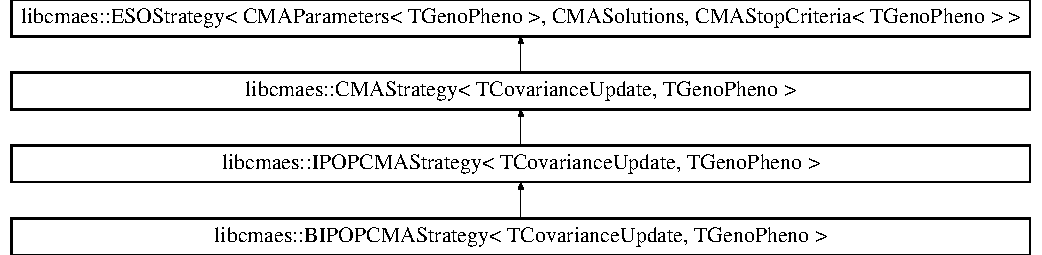
\includegraphics[height=1.429301cm]{classlibcmaes_1_1CMAStrategy}
\end{center}
\end{figure}
\subsection*{Public Member Functions}
\begin{DoxyCompactItemize}
\item 
\hypertarget{classlibcmaes_1_1CMAStrategy_a855fbfb7dd9745ea764648f8965d1f3e}{\hyperlink{classlibcmaes_1_1CMAStrategy_a855fbfb7dd9745ea764648f8965d1f3e}{C\-M\-A\-Strategy} ()}\label{classlibcmaes_1_1CMAStrategy_a855fbfb7dd9745ea764648f8965d1f3e}

\begin{DoxyCompactList}\small\item\em dummy constructor \end{DoxyCompactList}\item 
\hyperlink{classlibcmaes_1_1CMAStrategy_a5455e7245be35c169e4144eb666f94f3}{C\-M\-A\-Strategy} (Fit\-Func \&func, \hyperlink{classlibcmaes_1_1CMAParameters}{C\-M\-A\-Parameters}$<$ T\-Geno\-Pheno $>$ \&parameters)
\begin{DoxyCompactList}\small\item\em constructor. \end{DoxyCompactList}\item 
\hyperlink{classlibcmaes_1_1CMAStrategy_a30decb362a4dd4c9557f0989d618aa93}{C\-M\-A\-Strategy} (Fit\-Func \&func, \hyperlink{classlibcmaes_1_1CMAParameters}{C\-M\-A\-Parameters}$<$ T\-Geno\-Pheno $>$ \&parameters, const \hyperlink{classlibcmaes_1_1CMASolutions}{C\-M\-A\-Solutions} \&cmasols)
\begin{DoxyCompactList}\small\item\em constructor for starting from an existing solution. \end{DoxyCompactList}\item 
\hypertarget{classlibcmaes_1_1CMAStrategy_ab7266bc50732458ffcab690bc26380e6}{d\-Mat \hyperlink{classlibcmaes_1_1CMAStrategy_ab7266bc50732458ffcab690bc26380e6}{ask} ()}\label{classlibcmaes_1_1CMAStrategy_ab7266bc50732458ffcab690bc26380e6}

\begin{DoxyCompactList}\small\item\em generates nsols new candidate solutions, sampled from a multivariate normal distribution. return \hyperlink{classA}{A} matrix whose rows contain the candidate points. \end{DoxyCompactList}\item 
\hypertarget{classlibcmaes_1_1CMAStrategy_a03d9a4f9338ccd55141323ca309dbdfa}{void \hyperlink{classlibcmaes_1_1CMAStrategy_a03d9a4f9338ccd55141323ca309dbdfa}{tell} ()}\label{classlibcmaes_1_1CMAStrategy_a03d9a4f9338ccd55141323ca309dbdfa}

\begin{DoxyCompactList}\small\item\em Updates the covariance matrix and prepares for the next iteration. \end{DoxyCompactList}\item 
bool \hyperlink{classlibcmaes_1_1CMAStrategy_adc87b9c500959c800b6bc93d89432ecc}{stop} ()
\begin{DoxyCompactList}\small\item\em Stops search on a set of termination criterias, see reference paper. \end{DoxyCompactList}\item 
int \hyperlink{classlibcmaes_1_1CMAStrategy_a920d0459bf636132528e81736175a1d9}{optimize} (const Eval\-Func \&evalf, const Ask\-Func \&askf, const Tell\-Func \&tellf)
\begin{DoxyCompactList}\small\item\em Finds the minimum of the objective function. It makes alternate calls to \hyperlink{classlibcmaes_1_1CMAStrategy_ab7266bc50732458ffcab690bc26380e6}{ask()}, \hyperlink{classlibcmaes_1_1CMAStrategy_a03d9a4f9338ccd55141323ca309dbdfa}{tell()} and \hyperlink{classlibcmaes_1_1CMAStrategy_adc87b9c500959c800b6bc93d89432ecc}{stop()} until one of the termination criteria triggers. \end{DoxyCompactList}\item 
int \hyperlink{classlibcmaes_1_1CMAStrategy_a68cb0023f51e2824758b1bd1c7512f39}{optimize} ()
\begin{DoxyCompactList}\small\item\em Finds the minimum of the objective function. It makes alternate calls to \hyperlink{classlibcmaes_1_1CMAStrategy_ab7266bc50732458ffcab690bc26380e6}{ask()}, \hyperlink{classlibcmaes_1_1CMAStrategy_a03d9a4f9338ccd55141323ca309dbdfa}{tell()} and \hyperlink{classlibcmaes_1_1CMAStrategy_adc87b9c500959c800b6bc93d89432ecc}{stop()} until one of the termination criteria triggers. \end{DoxyCompactList}\item 
\hypertarget{classlibcmaes_1_1CMAStrategy_a5e56719b620697538d5abe52b5f59b67}{void \hyperlink{classlibcmaes_1_1CMAStrategy_a5e56719b620697538d5abe52b5f59b67}{plot} ()}\label{classlibcmaes_1_1CMAStrategy_a5e56719b620697538d5abe52b5f59b67}

\begin{DoxyCompactList}\small\item\em Stream the internal state of the search into an output file, as defined in the \-\_\-parameters object. \end{DoxyCompactList}\end{DoxyCompactItemize}
\subsection*{Static Public Attributes}
\begin{DoxyCompactItemize}
\item 
static Progress\-Func\\*
$<$ \hyperlink{classlibcmaes_1_1CMAParameters}{C\-M\-A\-Parameters}$<$ T\-Geno\-Pheno $>$\\*
, \hyperlink{classlibcmaes_1_1CMASolutions}{C\-M\-A\-Solutions} $>$ \hyperlink{classlibcmaes_1_1CMAStrategy_af6d980c670eef47ee810645739999d5b}{\-\_\-default\-P\-Func}
\item 
static Plot\-Func$<$ \hyperlink{classlibcmaes_1_1CMAParameters}{C\-M\-A\-Parameters}\\*
$<$ T\-Geno\-Pheno $>$, \hyperlink{classlibcmaes_1_1CMASolutions}{C\-M\-A\-Solutions} $>$ \hyperlink{classlibcmaes_1_1CMAStrategy_a0fcdccd9451a2dc509ee651f664ac31f}{\-\_\-default\-F\-P\-Func}
\end{DoxyCompactItemize}
\subsection*{Protected Attributes}
\begin{DoxyCompactItemize}
\item 
\hyperlink{classEigen_1_1EigenMultivariateNormal}{Eigen\-::\-Eigen\-Multivariate\-Normal}\\*
$<$ double $>$ \hyperlink{classlibcmaes_1_1CMAStrategy_ad9d6fe34da1fb94315e86625210fe009}{\-\_\-esolver}
\item 
\hyperlink{classlibcmaes_1_1CMAStopCriteria}{C\-M\-A\-Stop\-Criteria}$<$ T\-Geno\-Pheno $>$ \hyperlink{classlibcmaes_1_1CMAStrategy_af7b7c6bf3018f5e3d57f2875215bba0c}{\-\_\-stopcriteria}
\item 
std\-::ofstream $\ast$ \hyperlink{classlibcmaes_1_1CMAStrategy_ad05db57e25a5aa2d4abe9cb030406236}{\-\_\-fplotstream} = nullptr
\end{DoxyCompactItemize}


\subsection{Detailed Description}
\subsubsection*{template$<$class T\-Covariance\-Update, class T\-Geno\-Pheno = Geno\-Pheno$<$\-No\-Bound\-Strategy$>$$>$class libcmaes\-::\-C\-M\-A\-Strategy$<$ T\-Covariance\-Update, T\-Geno\-Pheno $>$}

This is an implementation of C\-M\-A-\/\-E\-S. It uses the reference algorithm and termination criteria of the following paper\-: Hansen, N. (2009). Benchmarking a B\-I-\/\-Population C\-M\-A-\/\-E\-S on the B\-B\-O\-B-\/2009 Function Testbed. Workshop Proceedings of the G\-E\-C\-C\-O Genetic and Evolutionary Computation Conference, A\-C\-M, pp. 2389-\/2395 See \href{https://www.lri.fr/~hansen/publications.html}{\tt https\-://www.\-lri.\-fr/$\sim$hansen/publications.\-html} for more information. 

\subsection{Constructor \& Destructor Documentation}
\hypertarget{classlibcmaes_1_1CMAStrategy_a5455e7245be35c169e4144eb666f94f3}{\index{libcmaes\-::\-C\-M\-A\-Strategy@{libcmaes\-::\-C\-M\-A\-Strategy}!C\-M\-A\-Strategy@{C\-M\-A\-Strategy}}
\index{C\-M\-A\-Strategy@{C\-M\-A\-Strategy}!libcmaes::CMAStrategy@{libcmaes\-::\-C\-M\-A\-Strategy}}
\subsubsection[{C\-M\-A\-Strategy}]{\setlength{\rightskip}{0pt plus 5cm}template$<$class T\-Covariance\-Update , class T\-Geno\-Pheno$>$ {\bf libcmaes\-::\-C\-M\-A\-Strategy}$<$ T\-Covariance\-Update, T\-Geno\-Pheno $>$\-::{\bf C\-M\-A\-Strategy} (
\begin{DoxyParamCaption}
\item[{Fit\-Func \&}]{func, }
\item[{{\bf C\-M\-A\-Parameters}$<$ T\-Geno\-Pheno $>$ \&}]{parameters}
\end{DoxyParamCaption}
)}}\label{classlibcmaes_1_1CMAStrategy_a5455e7245be35c169e4144eb666f94f3}


constructor. 


\begin{DoxyParams}{Parameters}
{\em func} & objective function to minimize \\
\hline
{\em parameters} & stochastic search parameters \\
\hline
\end{DoxyParams}
\hypertarget{classlibcmaes_1_1CMAStrategy_a30decb362a4dd4c9557f0989d618aa93}{\index{libcmaes\-::\-C\-M\-A\-Strategy@{libcmaes\-::\-C\-M\-A\-Strategy}!C\-M\-A\-Strategy@{C\-M\-A\-Strategy}}
\index{C\-M\-A\-Strategy@{C\-M\-A\-Strategy}!libcmaes::CMAStrategy@{libcmaes\-::\-C\-M\-A\-Strategy}}
\subsubsection[{C\-M\-A\-Strategy}]{\setlength{\rightskip}{0pt plus 5cm}template$<$class T\-Covariance\-Update , class T\-Geno\-Pheno$>$ {\bf libcmaes\-::\-C\-M\-A\-Strategy}$<$ T\-Covariance\-Update, T\-Geno\-Pheno $>$\-::{\bf C\-M\-A\-Strategy} (
\begin{DoxyParamCaption}
\item[{Fit\-Func \&}]{func, }
\item[{{\bf C\-M\-A\-Parameters}$<$ T\-Geno\-Pheno $>$ \&}]{parameters, }
\item[{const {\bf C\-M\-A\-Solutions} \&}]{cmasols}
\end{DoxyParamCaption}
)}}\label{classlibcmaes_1_1CMAStrategy_a30decb362a4dd4c9557f0989d618aa93}


constructor for starting from an existing solution. 


\begin{DoxyParams}{Parameters}
{\em func} & objective function to minimize \\
\hline
{\em parameters} & stochastic search parameters \\
\hline
{\em cmasols} & solution object to start from \\
\hline
\end{DoxyParams}


\subsection{Member Function Documentation}
\hypertarget{classlibcmaes_1_1CMAStrategy_a920d0459bf636132528e81736175a1d9}{\index{libcmaes\-::\-C\-M\-A\-Strategy@{libcmaes\-::\-C\-M\-A\-Strategy}!optimize@{optimize}}
\index{optimize@{optimize}!libcmaes::CMAStrategy@{libcmaes\-::\-C\-M\-A\-Strategy}}
\subsubsection[{optimize}]{\setlength{\rightskip}{0pt plus 5cm}template$<$class T\-Covariance\-Update , class T\-Geno\-Pheno $>$ int {\bf libcmaes\-::\-C\-M\-A\-Strategy}$<$ T\-Covariance\-Update, T\-Geno\-Pheno $>$\-::optimize (
\begin{DoxyParamCaption}
\item[{const Eval\-Func \&}]{evalf, }
\item[{const Ask\-Func \&}]{askf, }
\item[{const Tell\-Func \&}]{tellf}
\end{DoxyParamCaption}
)}}\label{classlibcmaes_1_1CMAStrategy_a920d0459bf636132528e81736175a1d9}


Finds the minimum of the objective function. It makes alternate calls to \hyperlink{classlibcmaes_1_1CMAStrategy_ab7266bc50732458ffcab690bc26380e6}{ask()}, \hyperlink{classlibcmaes_1_1CMAStrategy_a03d9a4f9338ccd55141323ca309dbdfa}{tell()} and \hyperlink{classlibcmaes_1_1CMAStrategy_adc87b9c500959c800b6bc93d89432ecc}{stop()} until one of the termination criteria triggers. 


\begin{DoxyParams}{Parameters}
{\em evalf} & custom eval function \\
\hline
{\em askf} & custom ask function \\
\hline
{\em tellf} & custom tell function \\
\hline
\end{DoxyParams}
\begin{DoxyReturn}{Returns}
success or error code, as defined in \hyperlink{opti__err_8h_source}{opti\-\_\-err.\-h} Note\-: the termination criteria code is held by \-\_\-solutions.\-\_\-run\-\_\-status 
\end{DoxyReturn}
\hypertarget{classlibcmaes_1_1CMAStrategy_a68cb0023f51e2824758b1bd1c7512f39}{\index{libcmaes\-::\-C\-M\-A\-Strategy@{libcmaes\-::\-C\-M\-A\-Strategy}!optimize@{optimize}}
\index{optimize@{optimize}!libcmaes::CMAStrategy@{libcmaes\-::\-C\-M\-A\-Strategy}}
\subsubsection[{optimize}]{\setlength{\rightskip}{0pt plus 5cm}template$<$class T\-Covariance\-Update, class T\-Geno\-Pheno = Geno\-Pheno$<$\-No\-Bound\-Strategy$>$$>$ int {\bf libcmaes\-::\-C\-M\-A\-Strategy}$<$ T\-Covariance\-Update, T\-Geno\-Pheno $>$\-::optimize (
\begin{DoxyParamCaption}
{}
\end{DoxyParamCaption}
)\hspace{0.3cm}{\ttfamily [inline]}}}\label{classlibcmaes_1_1CMAStrategy_a68cb0023f51e2824758b1bd1c7512f39}


Finds the minimum of the objective function. It makes alternate calls to \hyperlink{classlibcmaes_1_1CMAStrategy_ab7266bc50732458ffcab690bc26380e6}{ask()}, \hyperlink{classlibcmaes_1_1CMAStrategy_a03d9a4f9338ccd55141323ca309dbdfa}{tell()} and \hyperlink{classlibcmaes_1_1CMAStrategy_adc87b9c500959c800b6bc93d89432ecc}{stop()} until one of the termination criteria triggers. 

\begin{DoxyReturn}{Returns}
success or error code, as defined in \hyperlink{opti__err_8h_source}{opti\-\_\-err.\-h} Note\-: the termination criteria code is held by \-\_\-solutions.\-\_\-run\-\_\-status 
\end{DoxyReturn}
\hypertarget{classlibcmaes_1_1CMAStrategy_adc87b9c500959c800b6bc93d89432ecc}{\index{libcmaes\-::\-C\-M\-A\-Strategy@{libcmaes\-::\-C\-M\-A\-Strategy}!stop@{stop}}
\index{stop@{stop}!libcmaes::CMAStrategy@{libcmaes\-::\-C\-M\-A\-Strategy}}
\subsubsection[{stop}]{\setlength{\rightskip}{0pt plus 5cm}template$<$class T\-Covariance\-Update , class T\-Geno\-Pheno $>$ bool {\bf libcmaes\-::\-C\-M\-A\-Strategy}$<$ T\-Covariance\-Update, T\-Geno\-Pheno $>$\-::stop (
\begin{DoxyParamCaption}
{}
\end{DoxyParamCaption}
)}}\label{classlibcmaes_1_1CMAStrategy_adc87b9c500959c800b6bc93d89432ecc}


Stops search on a set of termination criterias, see reference paper. 

\begin{DoxyReturn}{Returns}
true if search must stop, false otherwise. 
\end{DoxyReturn}


\subsection{Member Data Documentation}
\hypertarget{classlibcmaes_1_1CMAStrategy_a0fcdccd9451a2dc509ee651f664ac31f}{\index{libcmaes\-::\-C\-M\-A\-Strategy@{libcmaes\-::\-C\-M\-A\-Strategy}!\-\_\-default\-F\-P\-Func@{\-\_\-default\-F\-P\-Func}}
\index{\-\_\-default\-F\-P\-Func@{\-\_\-default\-F\-P\-Func}!libcmaes::CMAStrategy@{libcmaes\-::\-C\-M\-A\-Strategy}}
\subsubsection[{\-\_\-default\-F\-P\-Func}]{\setlength{\rightskip}{0pt plus 5cm}template$<$class T\-Covariance\-Update, class T\-Geno\-Pheno = Geno\-Pheno$<$\-No\-Bound\-Strategy$>$$>$ Plot\-Func$<$ {\bf C\-M\-A\-Parameters}$<$ T\-Geno\-Pheno $>$, {\bf C\-M\-A\-Solutions} $>$ {\bf libcmaes\-::\-C\-M\-A\-Strategy}$<$ T\-Covariance\-Update, T\-Geno\-Pheno $>$\-::\-\_\-default\-F\-P\-Func\hspace{0.3cm}{\ttfamily [static]}}}\label{classlibcmaes_1_1CMAStrategy_a0fcdccd9451a2dc509ee651f664ac31f}
{\bfseries Initial value\-:}
\begin{DoxyCode}
= [](\textcolor{keyword}{const} CMAParameters<TGenoPheno> &cmaparams, \textcolor{keyword}{const} CMASolutions &cmasols, std::ofstream &fplotstream)
  \{
    std::string sep = \textcolor{stringliteral}{" "};
    fplotstream << fabs(cmasols.best\_candidate().get\_fvalue()) << sep << cmasols.fevals() << sep << cmasols
      .sigma() << sep << sqrt(cmasols.max\_eigenv()/cmasols.min\_eigenv()) << sep;
    fplotstream << cmasols.eigenvalues().transpose() << sep;
    \textcolor{keywordflow}{if} (!cmaparams.is\_sep() && !cmaparams.is\_vd())
      fplotstream << cmasols.cov().sqrt().diagonal().transpose() << sep; 
    \textcolor{keywordflow}{else} \textcolor{keywordflow}{if} (cmaparams.is\_sep())
      fplotstream << cmasols.sepcov().cwiseSqrt().transpose() << sep;
    \textcolor{keywordflow}{else} \textcolor{keywordflow}{if} (cmaparams.is\_vd())
      fplotstream << cmasols.sepcov().transpose() << sep; 
    fplotstream << cmaparams.get\_gp().pheno(cmasols.xmean()).transpose();
    fplotstream << sep << cmasols.elapsed\_last\_iter();



    fplotstream << std::endl;
    \textcolor{keywordflow}{return} 0;
  \}
\end{DoxyCode}
the default plot to file function. \hypertarget{classlibcmaes_1_1CMAStrategy_af6d980c670eef47ee810645739999d5b}{\index{libcmaes\-::\-C\-M\-A\-Strategy@{libcmaes\-::\-C\-M\-A\-Strategy}!\-\_\-default\-P\-Func@{\-\_\-default\-P\-Func}}
\index{\-\_\-default\-P\-Func@{\-\_\-default\-P\-Func}!libcmaes::CMAStrategy@{libcmaes\-::\-C\-M\-A\-Strategy}}
\subsubsection[{\-\_\-default\-P\-Func}]{\setlength{\rightskip}{0pt plus 5cm}template$<$class T\-Covariance\-Update, class T\-Geno\-Pheno = Geno\-Pheno$<$\-No\-Bound\-Strategy$>$$>$ Progress\-Func$<$ {\bf C\-M\-A\-Parameters}$<$ T\-Geno\-Pheno $>$, {\bf C\-M\-A\-Solutions} $>$ {\bf libcmaes\-::\-C\-M\-A\-Strategy}$<$ T\-Covariance\-Update, T\-Geno\-Pheno $>$\-::\-\_\-default\-P\-Func\hspace{0.3cm}{\ttfamily [static]}}}\label{classlibcmaes_1_1CMAStrategy_af6d980c670eef47ee810645739999d5b}
{\bfseries Initial value\-:}
\begin{DoxyCode}
= [](\textcolor{keyword}{const} CMAParameters<TGenoPheno> &cmaparams, \textcolor{keyword}{const} CMASolutions &cmasols)
  \{
    LOG\_IF(INFO,!cmaparams.quiet()) << std::setprecision(std::numeric\_limits<double>::digits10) << \textcolor{stringliteral}{"iter="} 
      << cmasols.niter() << \textcolor{stringliteral}{" / evals="} << cmasols.fevals() << \textcolor{stringliteral}{" / f-value="} << cmasols.best\_candidate().
      get\_fvalue() <<  \textcolor{stringliteral}{" / sigma="} << cmasols.sigma() << \textcolor{stringliteral}{" / last\_iter="} << cmasols.elapsed\_last\_iter() << std::endl;
    \textcolor{keywordflow}{return} 0;
  \}
\end{DoxyCode}
the default progress function. \hypertarget{classlibcmaes_1_1CMAStrategy_ad9d6fe34da1fb94315e86625210fe009}{\index{libcmaes\-::\-C\-M\-A\-Strategy@{libcmaes\-::\-C\-M\-A\-Strategy}!\-\_\-esolver@{\-\_\-esolver}}
\index{\-\_\-esolver@{\-\_\-esolver}!libcmaes::CMAStrategy@{libcmaes\-::\-C\-M\-A\-Strategy}}
\subsubsection[{\-\_\-esolver}]{\setlength{\rightskip}{0pt plus 5cm}template$<$class T\-Covariance\-Update, class T\-Geno\-Pheno = Geno\-Pheno$<$\-No\-Bound\-Strategy$>$$>$ {\bf Eigen\-::\-Eigen\-Multivariate\-Normal}$<$double$>$ {\bf libcmaes\-::\-C\-M\-A\-Strategy}$<$ T\-Covariance\-Update, T\-Geno\-Pheno $>$\-::\-\_\-esolver\hspace{0.3cm}{\ttfamily [protected]}}}\label{classlibcmaes_1_1CMAStrategy_ad9d6fe34da1fb94315e86625210fe009}
multivariate normal distribution sampler, and eigendecomposition solver. \hypertarget{classlibcmaes_1_1CMAStrategy_ad05db57e25a5aa2d4abe9cb030406236}{\index{libcmaes\-::\-C\-M\-A\-Strategy@{libcmaes\-::\-C\-M\-A\-Strategy}!\-\_\-fplotstream@{\-\_\-fplotstream}}
\index{\-\_\-fplotstream@{\-\_\-fplotstream}!libcmaes::CMAStrategy@{libcmaes\-::\-C\-M\-A\-Strategy}}
\subsubsection[{\-\_\-fplotstream}]{\setlength{\rightskip}{0pt plus 5cm}template$<$class T\-Covariance\-Update, class T\-Geno\-Pheno = Geno\-Pheno$<$\-No\-Bound\-Strategy$>$$>$ std\-::ofstream$\ast$ {\bf libcmaes\-::\-C\-M\-A\-Strategy}$<$ T\-Covariance\-Update, T\-Geno\-Pheno $>$\-::\-\_\-fplotstream = nullptr\hspace{0.3cm}{\ttfamily [protected]}}}\label{classlibcmaes_1_1CMAStrategy_ad05db57e25a5aa2d4abe9cb030406236}
plotting file stream, not in parameters because of copy-\/constructor hell. \hypertarget{classlibcmaes_1_1CMAStrategy_af7b7c6bf3018f5e3d57f2875215bba0c}{\index{libcmaes\-::\-C\-M\-A\-Strategy@{libcmaes\-::\-C\-M\-A\-Strategy}!\-\_\-stopcriteria@{\-\_\-stopcriteria}}
\index{\-\_\-stopcriteria@{\-\_\-stopcriteria}!libcmaes::CMAStrategy@{libcmaes\-::\-C\-M\-A\-Strategy}}
\subsubsection[{\-\_\-stopcriteria}]{\setlength{\rightskip}{0pt plus 5cm}template$<$class T\-Covariance\-Update, class T\-Geno\-Pheno = Geno\-Pheno$<$\-No\-Bound\-Strategy$>$$>$ {\bf C\-M\-A\-Stop\-Criteria}$<$T\-Geno\-Pheno$>$ {\bf libcmaes\-::\-C\-M\-A\-Strategy}$<$ T\-Covariance\-Update, T\-Geno\-Pheno $>$\-::\-\_\-stopcriteria\hspace{0.3cm}{\ttfamily [protected]}}}\label{classlibcmaes_1_1CMAStrategy_af7b7c6bf3018f5e3d57f2875215bba0c}
holds the set of termination criteria, see reference paper. 

The documentation for this class was generated from the following files\-:\begin{DoxyCompactItemize}
\item 
src/cmastrategy.\-h\item 
src/cmastrategy.\-cc\end{DoxyCompactItemize}

\hypertarget{classlibcmaes_1_1CovarianceUpdate}{\section{libcmaes\+:\+:Covariance\+Update Class Reference}
\label{classlibcmaes_1_1CovarianceUpdate}\index{libcmaes\+::\+Covariance\+Update@{libcmaes\+::\+Covariance\+Update}}
}


Covariance Matrix update. This is an implementation closely follows\+: Hansen, N. (2009). Benchmarking a B\+I-\/\+Population C\+M\+A-\/\+E\+S on the B\+B\+O\+B-\/2009 Function Testbed. Workshop Proceedings of the G\+E\+C\+C\+O Genetic and Evolutionary Computation Conference, A\+C\+M, pp. 2389-\/2395.  




{\ttfamily \#include $<$covarianceupdate.\+h$>$}

\subsection*{Static Public Member Functions}
\begin{DoxyCompactItemize}
\item 
{\footnotesize template$<$class T\+Geno\+Pheno $>$ }\\static void \hyperlink{classlibcmaes_1_1CovarianceUpdate_a39f58b771690547822ad54b8e89201cd}{update} (const \hyperlink{classlibcmaes_1_1CMAParameters}{C\+M\+A\+Parameters}$<$ T\+Geno\+Pheno $>$ \&parameters, \hyperlink{classEigen_1_1EigenMultivariateNormal}{Eigen\+::\+Eigen\+Multivariate\+Normal}$<$ double $>$ \&esolver, \hyperlink{classlibcmaes_1_1CMASolutions}{C\+M\+A\+Solutions} \&solutions)
\begin{DoxyCompactList}\small\item\em update the covariance matrix. \end{DoxyCompactList}\end{DoxyCompactItemize}


\subsection{Detailed Description}
Covariance Matrix update. This is an implementation closely follows\+: Hansen, N. (2009). Benchmarking a B\+I-\/\+Population C\+M\+A-\/\+E\+S on the B\+B\+O\+B-\/2009 Function Testbed. Workshop Proceedings of the G\+E\+C\+C\+O Genetic and Evolutionary Computation Conference, A\+C\+M, pp. 2389-\/2395. 

\subsection{Member Function Documentation}
\hypertarget{classlibcmaes_1_1CovarianceUpdate_a39f58b771690547822ad54b8e89201cd}{\index{libcmaes\+::\+Covariance\+Update@{libcmaes\+::\+Covariance\+Update}!update@{update}}
\index{update@{update}!libcmaes\+::\+Covariance\+Update@{libcmaes\+::\+Covariance\+Update}}
\subsubsection[{update}]{\setlength{\rightskip}{0pt plus 5cm}template$<$class T\+Geno\+Pheno $>$ template void libcmaes\+::\+Covariance\+Update\+::update (
\begin{DoxyParamCaption}
\item[{const {\bf C\+M\+A\+Parameters}$<$ T\+Geno\+Pheno $>$ \&}]{parameters, }
\item[{{\bf Eigen\+::\+Eigen\+Multivariate\+Normal}$<$ double $>$ \&}]{esolver, }
\item[{{\bf C\+M\+A\+Solutions} \&}]{solutions}
\end{DoxyParamCaption}
)\hspace{0.3cm}{\ttfamily [static]}}}\label{classlibcmaes_1_1CovarianceUpdate_a39f58b771690547822ad54b8e89201cd}


update the covariance matrix. 


\begin{DoxyParams}{Parameters}
{\em parameters} & current set of parameters \\
\hline
{\em esolver} & \hyperlink{namespaceEigen}{Eigen} eigenvalue solver \\
\hline
{\em solutions} & currrent set of solutions. \\
\hline
\end{DoxyParams}


The documentation for this class was generated from the following files\+:\begin{DoxyCompactItemize}
\item 
src/covarianceupdate.\+h\item 
src/covarianceupdate.\+cc\end{DoxyCompactItemize}

\hypertarget{classcustomCMAStrategy}{\section{custom\+C\+M\+A\+Strategy Class Reference}
\label{classcustomCMAStrategy}\index{custom\+C\+M\+A\+Strategy@{custom\+C\+M\+A\+Strategy}}
}
Inheritance diagram for custom\+C\+M\+A\+Strategy\+:\begin{figure}[H]
\begin{center}
\leavevmode
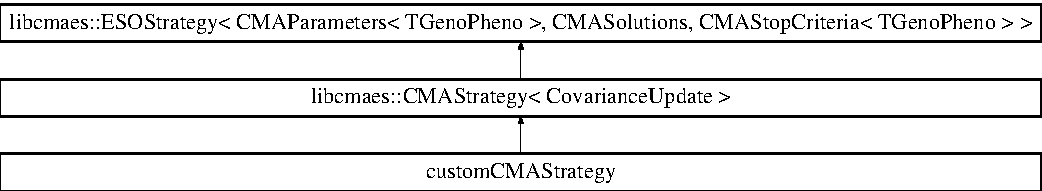
\includegraphics[height=2.572741cm]{classcustomCMAStrategy}
\end{center}
\end{figure}
\subsection*{Public Member Functions}
\begin{DoxyCompactItemize}
\item 
\hypertarget{classcustomCMAStrategy_a8d471b2aaca71aef766ce1030b20ae58}{{\bfseries custom\+C\+M\+A\+Strategy} (Fit\+Func \&func, \hyperlink{classlibcmaes_1_1CMAParameters}{C\+M\+A\+Parameters}$<$$>$ \&parameters)}\label{classcustomCMAStrategy_a8d471b2aaca71aef766ce1030b20ae58}

\item 
\hypertarget{classcustomCMAStrategy_a1c611a946b6252688edfc680ad2745c6}{d\+Mat {\bfseries ask} ()}\label{classcustomCMAStrategy_a1c611a946b6252688edfc680ad2745c6}

\item 
\hypertarget{classcustomCMAStrategy_ad88a47f2d2d7c01ad7196442181c61c3}{void {\bfseries eval} (const d\+Mat \&candidates, const d\+Mat \&phenocandidates=d\+Mat(0, 0))}\label{classcustomCMAStrategy_ad88a47f2d2d7c01ad7196442181c61c3}

\item 
\hypertarget{classcustomCMAStrategy_a45d116c8f308da33df7de95d8b0fc9a7}{void {\bfseries tell} ()}\label{classcustomCMAStrategy_a45d116c8f308da33df7de95d8b0fc9a7}

\item 
\hypertarget{classcustomCMAStrategy_ad600466db80f4a4692f66477529a457f}{bool {\bfseries stop} ()}\label{classcustomCMAStrategy_ad600466db80f4a4692f66477529a457f}

\end{DoxyCompactItemize}
\subsection*{Additional Inherited Members}


The documentation for this class was generated from the following file\+:\begin{DoxyCompactItemize}
\item 
examples/sample-\/code-\/ask-\/tell.\+cc\end{DoxyCompactItemize}

\hypertarget{classEigen_1_1EigenMultivariateNormal}{\section{Eigen\+:\+:Eigen\+Multivariate\+Normal$<$ Scalar $>$ Class Template Reference}
\label{classEigen_1_1EigenMultivariateNormal}\index{Eigen\+::\+Eigen\+Multivariate\+Normal$<$ Scalar $>$@{Eigen\+::\+Eigen\+Multivariate\+Normal$<$ Scalar $>$}}
}


{\ttfamily \#include $<$eigenmvn.\+h$>$}

\subsection*{Public Member Functions}
\begin{DoxyCompactItemize}
\item 
\hypertarget{classEigen_1_1EigenMultivariateNormal_a5c226d14c6597ad2314a2730f9b2e402}{void {\bfseries set\+\_\+covar} (const Matrix$<$ Scalar, Dynamic, Dynamic $>$ \&covar)}\label{classEigen_1_1EigenMultivariateNormal_a5c226d14c6597ad2314a2730f9b2e402}

\item 
\hypertarget{classEigen_1_1EigenMultivariateNormal_a05fa9ab49cb21d677c7ed84a276964a7}{void {\bfseries set\+\_\+transform} (const Matrix$<$ Scalar, Dynamic, Dynamic $>$ \&transform)}\label{classEigen_1_1EigenMultivariateNormal_a05fa9ab49cb21d677c7ed84a276964a7}

\item 
\hypertarget{classEigen_1_1EigenMultivariateNormal_ad8dc1c371b98d343741f144a3babef91}{{\bfseries Eigen\+Multivariate\+Normal} (const bool \&use\+\_\+cholesky=false, const uint64\+\_\+t \&seed=std\+::mt19937\+::default\+\_\+seed)}\label{classEigen_1_1EigenMultivariateNormal_ad8dc1c371b98d343741f144a3babef91}

\item 
\hypertarget{classEigen_1_1EigenMultivariateNormal_a427929ac9e14e93d56ec6acdb85a8dbb}{{\bfseries Eigen\+Multivariate\+Normal} (const Matrix$<$ Scalar, Dynamic, 1 $>$ \&mean, const Matrix$<$ Scalar, Dynamic, Dynamic $>$ \&covar, const bool \&use\+\_\+cholesky=false, const uint64\+\_\+t \&seed=std\+::mt19937\+::default\+\_\+seed)}\label{classEigen_1_1EigenMultivariateNormal_a427929ac9e14e93d56ec6acdb85a8dbb}

\item 
\hypertarget{classEigen_1_1EigenMultivariateNormal_aa9b735112cea507cd0a5f0eeffafe3c2}{void {\bfseries set\+Mean} (const Matrix$<$ Scalar, Dynamic, 1 $>$ \&mean)}\label{classEigen_1_1EigenMultivariateNormal_aa9b735112cea507cd0a5f0eeffafe3c2}

\item 
\hypertarget{classEigen_1_1EigenMultivariateNormal_a56942d3a51cf934f85d5b95275da9d18}{void {\bfseries set\+Covar} (const Matrix$<$ Scalar, Dynamic, Dynamic $>$ \&covar)}\label{classEigen_1_1EigenMultivariateNormal_a56942d3a51cf934f85d5b95275da9d18}

\item 
Matrix$<$ Scalar, Dynamic,-\/1 $>$ \hyperlink{classEigen_1_1EigenMultivariateNormal_a0a0c8f8310e6469b3365e735e95c9c87}{samples} (int nn, double factor)
\item 
\hypertarget{classEigen_1_1EigenMultivariateNormal_a957ca8e363a84616c1cb235d595fbfcd}{Matrix$<$ Scalar, Dynamic,-\/1 $>$ {\bfseries samples\+\_\+ind} (int nn, double factor)}\label{classEigen_1_1EigenMultivariateNormal_a957ca8e363a84616c1cb235d595fbfcd}

\item 
\hypertarget{classEigen_1_1EigenMultivariateNormal_ac81198e693bee0a5b350cec5c8293897}{Matrix$<$ Scalar, Dynamic,-\/1 $>$ {\bfseries samples\+\_\+ind} (int nn)}\label{classEigen_1_1EigenMultivariateNormal_ac81198e693bee0a5b350cec5c8293897}

\end{DoxyCompactItemize}
\subsection*{Public Attributes}
\begin{DoxyCompactItemize}
\item 
\hypertarget{classEigen_1_1EigenMultivariateNormal_aceef5dd5ce5aee926fab9f051cd8904b}{Self\+Adjoint\+Eigen\+Solver$<$ Matrix\\*
$<$ Scalar, Dynamic, Dynamic $>$ $>$ {\bfseries \+\_\+eigen\+Solver}}\label{classEigen_1_1EigenMultivariateNormal_aceef5dd5ce5aee926fab9f051cd8904b}

\end{DoxyCompactItemize}


\subsection{Detailed Description}
\subsubsection*{template$<$typename Scalar$>$class Eigen\+::\+Eigen\+Multivariate\+Normal$<$ Scalar $>$}

Find the eigen-\/decomposition of the covariance matrix and then store it for sampling from a multi-\/variate normal 

\subsection{Member Function Documentation}
\hypertarget{classEigen_1_1EigenMultivariateNormal_a0a0c8f8310e6469b3365e735e95c9c87}{\index{Eigen\+::\+Eigen\+Multivariate\+Normal@{Eigen\+::\+Eigen\+Multivariate\+Normal}!samples@{samples}}
\index{samples@{samples}!Eigen\+::\+Eigen\+Multivariate\+Normal@{Eigen\+::\+Eigen\+Multivariate\+Normal}}
\subsubsection[{samples}]{\setlength{\rightskip}{0pt plus 5cm}template$<$typename Scalar$>$ Matrix$<$Scalar,Dynamic,-\/1$>$ {\bf Eigen\+::\+Eigen\+Multivariate\+Normal}$<$ Scalar $>$\+::samples (
\begin{DoxyParamCaption}
\item[{int}]{nn, }
\item[{double}]{factor}
\end{DoxyParamCaption}
)\hspace{0.3cm}{\ttfamily [inline]}}}\label{classEigen_1_1EigenMultivariateNormal_a0a0c8f8310e6469b3365e735e95c9c87}
Draw nn samples from the gaussian and return them as columns in a Dynamic by nn matrix 

The documentation for this class was generated from the following file\+:\begin{DoxyCompactItemize}
\item 
src/eigenmvn.\+h\end{DoxyCompactItemize}

\hypertarget{classlibcmaes_1_1ESOptimizer}{\section{libcmaes\-:\-:E\-S\-Optimizer$<$ T\-E\-S\-O\-Strategy, T\-Parameters $>$ Class Template Reference}
\label{classlibcmaes_1_1ESOptimizer}\index{libcmaes\-::\-E\-S\-Optimizer$<$ T\-E\-S\-O\-Strategy, T\-Parameters $>$@{libcmaes\-::\-E\-S\-Optimizer$<$ T\-E\-S\-O\-Strategy, T\-Parameters $>$}}
}


an optimizer main class.  




{\ttfamily \#include $<$esoptimizer.\-h$>$}

Inheritance diagram for libcmaes\-:\-:E\-S\-Optimizer$<$ T\-E\-S\-O\-Strategy, T\-Parameters $>$\-:\begin{figure}[H]
\begin{center}
\leavevmode
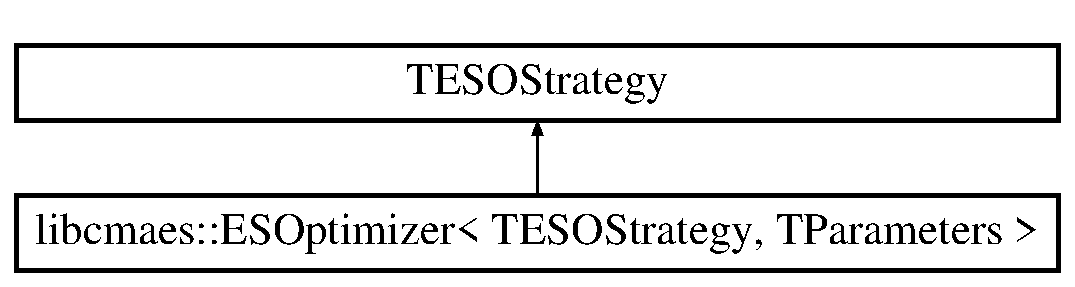
\includegraphics[height=2.000000cm]{classlibcmaes_1_1ESOptimizer}
\end{center}
\end{figure}
\subsection*{Public Member Functions}
\begin{DoxyCompactItemize}
\item 
\hyperlink{classlibcmaes_1_1ESOptimizer_a7c58536329acf5c33e11b882130629d9}{E\-S\-Optimizer} (Fit\-Func \&func, T\-Parameters \&parameters)
\begin{DoxyCompactList}\small\item\em constructor \end{DoxyCompactList}\item 
\hypertarget{classlibcmaes_1_1ESOptimizer_a175e487b798d7a748c28c784256b51c8}{int \hyperlink{classlibcmaes_1_1ESOptimizer_a175e487b798d7a748c28c784256b51c8}{optimize} ()}\label{classlibcmaes_1_1ESOptimizer_a175e487b798d7a748c28c784256b51c8}

\begin{DoxyCompactList}\small\item\em finds the minimum of a function, by calling on the underlying procedure of the E\-O\-S\-Optimizer object, like a variety of flavor of C\-M\-A-\/\-E\-S. \end{DoxyCompactList}\end{DoxyCompactItemize}


\subsection{Detailed Description}
\subsubsection*{template$<$class T\-E\-S\-O\-Strategy, class T\-Parameters$>$class libcmaes\-::\-E\-S\-Optimizer$<$ T\-E\-S\-O\-Strategy, T\-Parameters $>$}

an optimizer main class. 

\subsection{Constructor \& Destructor Documentation}
\hypertarget{classlibcmaes_1_1ESOptimizer_a7c58536329acf5c33e11b882130629d9}{\index{libcmaes\-::\-E\-S\-Optimizer@{libcmaes\-::\-E\-S\-Optimizer}!E\-S\-Optimizer@{E\-S\-Optimizer}}
\index{E\-S\-Optimizer@{E\-S\-Optimizer}!libcmaes::ESOptimizer@{libcmaes\-::\-E\-S\-Optimizer}}
\subsubsection[{E\-S\-Optimizer}]{\setlength{\rightskip}{0pt plus 5cm}template$<$class T\-E\-S\-O\-Strategy , class T\-Parameters $>$ {\bf libcmaes\-::\-E\-S\-Optimizer}$<$ T\-E\-S\-O\-Strategy, T\-Parameters $>$\-::{\bf E\-S\-Optimizer} (
\begin{DoxyParamCaption}
\item[{Fit\-Func \&}]{func, }
\item[{T\-Parameters \&}]{parameters}
\end{DoxyParamCaption}
)\hspace{0.3cm}{\ttfamily [inline]}}}\label{classlibcmaes_1_1ESOptimizer_a7c58536329acf5c33e11b882130629d9}


constructor 


\begin{DoxyParams}{Parameters}
{\em func} & function to minimize \\
\hline
{\em parameters} & optimization parameters \\
\hline
\end{DoxyParams}


The documentation for this class was generated from the following file\-:\begin{DoxyCompactItemize}
\item 
src/esoptimizer.\-h\end{DoxyCompactItemize}

\hypertarget{classlibcmaes_1_1ESOStrategy}{\section{libcmaes\-:\-:E\-S\-O\-Strategy$<$ T\-Parameters, T\-Solutions, T\-Stop\-Criteria $>$ Class Template Reference}
\label{classlibcmaes_1_1ESOStrategy}\index{libcmaes\-::\-E\-S\-O\-Strategy$<$ T\-Parameters, T\-Solutions, T\-Stop\-Criteria $>$@{libcmaes\-::\-E\-S\-O\-Strategy$<$ T\-Parameters, T\-Solutions, T\-Stop\-Criteria $>$}}
}


Main class describing an evolutionary optimization strategy. Every algorithm in libcmaes descends from this class, and bring its functionalities to an \hyperlink{classlibcmaes_1_1ESOptimizer}{E\-S\-Optimizer} object.  




{\ttfamily \#include $<$esostrategy.\-h$>$}

\subsection*{Public Member Functions}
\begin{DoxyCompactItemize}
\item 
\hypertarget{classlibcmaes_1_1ESOStrategy_aeae9653bf7cec51980c239200ad5c3df}{\hyperlink{classlibcmaes_1_1ESOStrategy_aeae9653bf7cec51980c239200ad5c3df}{E\-S\-O\-Strategy} ()}\label{classlibcmaes_1_1ESOStrategy_aeae9653bf7cec51980c239200ad5c3df}

\begin{DoxyCompactList}\small\item\em dummy constructor. \end{DoxyCompactList}\item 
\hyperlink{classlibcmaes_1_1ESOStrategy_a3736c9ce43cf708675229ff7b3ae4166}{E\-S\-O\-Strategy} (Fit\-Func \&func, T\-Parameters \&parameters)
\begin{DoxyCompactList}\small\item\em constructor \end{DoxyCompactList}\item 
\hyperlink{classlibcmaes_1_1ESOStrategy_abb06d0491f0240f875f66e9a4863f467}{E\-S\-O\-Strategy} (Fit\-Func \&func, T\-Parameters \&parameters, const T\-Solutions \&solutions)
\begin{DoxyCompactList}\small\item\em constructor for starting from an existing solution. \end{DoxyCompactList}\item 
d\-Mat \hyperlink{classlibcmaes_1_1ESOStrategy_af614d71ca3e8353b3027723220c9e3b4}{ask} ()
\begin{DoxyCompactList}\small\item\em Generates a set of candidate points. \end{DoxyCompactList}\item 
void \hyperlink{classlibcmaes_1_1ESOStrategy_a5e2e44bd0808efa95feea7ff5ef7eb91}{eval} (const d\-Mat \&candidates, const d\-Mat \&phenocandidates=d\-Mat(0, 0))
\begin{DoxyCompactList}\small\item\em Evaluates a set of candidates against the objective function. The procedure is multithreaded and stores both the candidates and their f-\/value into the \-\_\-solutions object that bears the current set of potential solutions to the optimization problem. \end{DoxyCompactList}\item 
\hypertarget{classlibcmaes_1_1ESOStrategy_ad35926877abdaed3922b316f57723612}{void \hyperlink{classlibcmaes_1_1ESOStrategy_ad35926877abdaed3922b316f57723612}{tell} ()}\label{classlibcmaes_1_1ESOStrategy_ad35926877abdaed3922b316f57723612}

\begin{DoxyCompactList}\small\item\em Updates the state of the stochastic search, and prepares for the next iteration. \end{DoxyCompactList}\item 
bool \hyperlink{classlibcmaes_1_1ESOStrategy_aa99c52d17342902cc4dc9a863deb58e3}{stop} ()
\begin{DoxyCompactList}\small\item\em Decides whether to stop the search for solutions. \end{DoxyCompactList}\item 
int \hyperlink{classlibcmaes_1_1ESOStrategy_ab56253c2d7753bf42c11b20a0b543b8d}{optimize} (const Eval\-Func \&evalf, const Ask\-Func \&askf, const Tell\-Func \&tellf)
\begin{DoxyCompactList}\small\item\em Finds the minimum of the objective function. It makes alternative calls to \hyperlink{classlibcmaes_1_1ESOStrategy_af614d71ca3e8353b3027723220c9e3b4}{ask()}, \hyperlink{classlibcmaes_1_1ESOStrategy_ad35926877abdaed3922b316f57723612}{tell()} and \hyperlink{classlibcmaes_1_1ESOStrategy_aa99c52d17342902cc4dc9a863deb58e3}{stop()} until one of the termination criteria triggers. \end{DoxyCompactList}\item 
\hypertarget{classlibcmaes_1_1ESOStrategy_a8eda694f97058ca603f8f31e5bb1bc05}{void \hyperlink{classlibcmaes_1_1ESOStrategy_a8eda694f97058ca603f8f31e5bb1bc05}{inc\-\_\-iter} ()}\label{classlibcmaes_1_1ESOStrategy_a8eda694f97058ca603f8f31e5bb1bc05}

\begin{DoxyCompactList}\small\item\em increment iteration count. \end{DoxyCompactList}\item 
void \hyperlink{classlibcmaes_1_1ESOStrategy_a9cfe783dc0284fce441c8757cd5222c3}{update\-\_\-fevals} (const int \&evals)
\begin{DoxyCompactList}\small\item\em updates the consumed budget of objective function evaluations. \end{DoxyCompactList}\item 
void \hyperlink{classlibcmaes_1_1ESOStrategy_aecb8aeecb2053868a7d9237223067267}{set\-\_\-gradient\-\_\-func} (Grad\-Func \&gfunc)
\begin{DoxyCompactList}\small\item\em sets the gradient function, if available. \end{DoxyCompactList}\item 
void \hyperlink{classlibcmaes_1_1ESOStrategy_a9d44ba79106b6afbd5881c4f33800840}{set\-\_\-progress\-\_\-func} (Progress\-Func$<$ T\-Parameters, T\-Solutions $>$ \&pfunc)
\begin{DoxyCompactList}\small\item\em Sets the possibly custom progress function, that is called in between every search step, and gives an outside user a simple way to witness progress of the algorithm, as well as to add custom termination criteria. \end{DoxyCompactList}\item 
void \hyperlink{classlibcmaes_1_1ESOStrategy_afa0e2a388dae01ec485c3dd8d80bb5ed}{start\-\_\-from\-\_\-solution} (const T\-Solutions \&sol)
\begin{DoxyCompactList}\small\item\em starts optimization from a given solution object. \end{DoxyCompactList}\item 
void \hyperlink{classlibcmaes_1_1ESOStrategy_ac0cdfca8b5614843661af4153e8c6b51}{set\-\_\-plot\-\_\-func} (Plot\-Func$<$ T\-Parameters, T\-Solutions $>$ \&pffunc)
\begin{DoxyCompactList}\small\item\em Sets the possibly custom plot to file function, that is useful for storing into file various possibly custom variable values for each step until termination. \end{DoxyCompactList}\item 
d\-Vec \hyperlink{classlibcmaes_1_1ESOStrategy_a43bd0b30c43445bc4ee2257963eebf47}{gradf} (const d\-Vec \&x)
\begin{DoxyCompactList}\small\item\em returns numerical gradient of objective function at x. \end{DoxyCompactList}\item 
d\-Vec \hyperlink{classlibcmaes_1_1ESOStrategy_a8a0581ead7ca7fac1f414c92ed030317}{gradgp} (const d\-Vec \&x) const 
\begin{DoxyCompactList}\small\item\em returns the numerical gradient of the objective function in phenotype space \end{DoxyCompactList}\item 
double \hyperlink{classlibcmaes_1_1ESOStrategy_a6350c635353e7b54e78abb223a5d4029}{edm} ()
\begin{DoxyCompactList}\small\item\em computes expected distance to minimum (E\-D\-M). \end{DoxyCompactList}\item 
T\-Solutions \& \hyperlink{classlibcmaes_1_1ESOStrategy_a0efc59c0fb25005207381cd3c45cb778}{get\-\_\-solutions} ()
\begin{DoxyCompactList}\small\item\em returns reference to current solution object \end{DoxyCompactList}\item 
T\-Parameters \& \hyperlink{classlibcmaes_1_1ESOStrategy_a6941ee6debca9ce43fb56eea7206ea33}{get\-\_\-parameters} ()
\begin{DoxyCompactList}\small\item\em returns reference to current optimization parameters object \end{DoxyCompactList}\item 
double \hyperlink{classlibcmaes_1_1ESOStrategy_a2763e44feed5c7635338fedaecb83e23}{fitfunc} (const double $\ast$x, const int N)
\begin{DoxyCompactList}\small\item\em execute objective function \end{DoxyCompactList}\item 
\hypertarget{classlibcmaes_1_1ESOStrategy_a81441905608aba3daa6d60a78eb47763}{\hyperlink{classlibcmaes_1_1Candidate}{Candidate} {\bfseries best\-\_\-solution} () const }\label{classlibcmaes_1_1ESOStrategy_a81441905608aba3daa6d60a78eb47763}

\item 
\hypertarget{classlibcmaes_1_1ESOStrategy_a059cdb2676a9e9933ac8b9dad32a1938}{void {\bfseries set\-\_\-initial\-\_\-elitist} (const bool \&e)}\label{classlibcmaes_1_1ESOStrategy_a059cdb2676a9e9933ac8b9dad32a1938}

\end{DoxyCompactItemize}
\subsection*{Protected Attributes}
\begin{DoxyCompactItemize}
\item 
Fit\-Func \hyperlink{classlibcmaes_1_1ESOStrategy_a1a29d4c30bbdb6021920275e81fa4dc4}{\-\_\-func}
\item 
int \hyperlink{classlibcmaes_1_1ESOStrategy_a19667f1e69856e7cfd6219b63cbaa59d}{\-\_\-nevals}
\item 
int \hyperlink{classlibcmaes_1_1ESOStrategy_aaf5c063558da34826ea1f976423ccfbb}{\-\_\-niter}
\item 
T\-Solutions \hyperlink{classlibcmaes_1_1ESOStrategy_a8fe0f8dc2201951e9e4ed2768b5a09ab}{\-\_\-solutions}
\item 
T\-Parameters \hyperlink{classlibcmaes_1_1ESOStrategy_a295e49238ceef8f11b3fb35296a8364a}{\-\_\-parameters}
\item 
Progress\-Func$<$ T\-Parameters, \\*
T\-Solutions $>$ \hyperlink{classlibcmaes_1_1ESOStrategy_a25d597189596f434a2530887fddea189}{\-\_\-pfunc}
\item 
Grad\-Func \hyperlink{classlibcmaes_1_1ESOStrategy_a76926e49a2ca941a22362167bc230093}{\-\_\-gfunc} = nullptr
\item 
Plot\-Func$<$ T\-Parameters, T\-Solutions $>$ \hyperlink{classlibcmaes_1_1ESOStrategy_af2c9909de76f98e4b9c207bda577255d}{\-\_\-pffunc}
\item 
\hypertarget{classlibcmaes_1_1ESOStrategy_a3b59faa95ebae7336607b9b4ebd0c266}{Fit\-Func {\bfseries \-\_\-funcaux}}\label{classlibcmaes_1_1ESOStrategy_a3b59faa95ebae7336607b9b4ebd0c266}

\item 
bool \hyperlink{classlibcmaes_1_1ESOStrategy_a1ee27b35458c52501bebf5bdc42de385}{\-\_\-initial\-\_\-elitist} = false
\end{DoxyCompactItemize}


\subsection{Detailed Description}
\subsubsection*{template$<$class T\-Parameters, class T\-Solutions, class T\-Stop\-Criteria$>$class libcmaes\-::\-E\-S\-O\-Strategy$<$ T\-Parameters, T\-Solutions, T\-Stop\-Criteria $>$}

Main class describing an evolutionary optimization strategy. Every algorithm in libcmaes descends from this class, and bring its functionalities to an \hyperlink{classlibcmaes_1_1ESOptimizer}{E\-S\-Optimizer} object. 

\subsection{Constructor \& Destructor Documentation}
\hypertarget{classlibcmaes_1_1ESOStrategy_a3736c9ce43cf708675229ff7b3ae4166}{\index{libcmaes\-::\-E\-S\-O\-Strategy@{libcmaes\-::\-E\-S\-O\-Strategy}!E\-S\-O\-Strategy@{E\-S\-O\-Strategy}}
\index{E\-S\-O\-Strategy@{E\-S\-O\-Strategy}!libcmaes::ESOStrategy@{libcmaes\-::\-E\-S\-O\-Strategy}}
\subsubsection[{E\-S\-O\-Strategy}]{\setlength{\rightskip}{0pt plus 5cm}template$<$class T\-Parameters, class T\-Solutions , class T\-Stop\-Criteria $>$ {\bf libcmaes\-::\-E\-S\-O\-Strategy}$<$ T\-Parameters, T\-Solutions, T\-Stop\-Criteria $>$\-::{\bf E\-S\-O\-Strategy} (
\begin{DoxyParamCaption}
\item[{Fit\-Func \&}]{func, }
\item[{T\-Parameters \&}]{parameters}
\end{DoxyParamCaption}
)}}\label{classlibcmaes_1_1ESOStrategy_a3736c9ce43cf708675229ff7b3ae4166}


constructor 


\begin{DoxyParams}{Parameters}
{\em func} & function to minimize \\
\hline
{\em parameters} & optimization parameters \\
\hline
\end{DoxyParams}
\hypertarget{classlibcmaes_1_1ESOStrategy_abb06d0491f0240f875f66e9a4863f467}{\index{libcmaes\-::\-E\-S\-O\-Strategy@{libcmaes\-::\-E\-S\-O\-Strategy}!E\-S\-O\-Strategy@{E\-S\-O\-Strategy}}
\index{E\-S\-O\-Strategy@{E\-S\-O\-Strategy}!libcmaes::ESOStrategy@{libcmaes\-::\-E\-S\-O\-Strategy}}
\subsubsection[{E\-S\-O\-Strategy}]{\setlength{\rightskip}{0pt plus 5cm}template$<$class T\-Parameters, class T\-Solutions, class T\-Stop\-Criteria $>$ {\bf libcmaes\-::\-E\-S\-O\-Strategy}$<$ T\-Parameters, T\-Solutions, T\-Stop\-Criteria $>$\-::{\bf E\-S\-O\-Strategy} (
\begin{DoxyParamCaption}
\item[{Fit\-Func \&}]{func, }
\item[{T\-Parameters \&}]{parameters, }
\item[{const T\-Solutions \&}]{solutions}
\end{DoxyParamCaption}
)}}\label{classlibcmaes_1_1ESOStrategy_abb06d0491f0240f875f66e9a4863f467}


constructor for starting from an existing solution. 


\begin{DoxyParams}{Parameters}
{\em func} & objective function to minimize \\
\hline
{\em parameters} & stochastic search parameters \\
\hline
{\em solution} & solution object to start from \\
\hline
\end{DoxyParams}


\subsection{Member Function Documentation}
\hypertarget{classlibcmaes_1_1ESOStrategy_af614d71ca3e8353b3027723220c9e3b4}{\index{libcmaes\-::\-E\-S\-O\-Strategy@{libcmaes\-::\-E\-S\-O\-Strategy}!ask@{ask}}
\index{ask@{ask}!libcmaes::ESOStrategy@{libcmaes\-::\-E\-S\-O\-Strategy}}
\subsubsection[{ask}]{\setlength{\rightskip}{0pt plus 5cm}template$<$class T\-Parameters, class T\-Solutions, class T\-Stop\-Criteria$>$ d\-Mat {\bf libcmaes\-::\-E\-S\-O\-Strategy}$<$ T\-Parameters, T\-Solutions, T\-Stop\-Criteria $>$\-::ask (
\begin{DoxyParamCaption}
{}
\end{DoxyParamCaption}
)}}\label{classlibcmaes_1_1ESOStrategy_af614d71ca3e8353b3027723220c9e3b4}


Generates a set of candidate points. 

\begin{DoxyReturn}{Returns}
\hyperlink{classA}{A} matrix whose rows contain the candidate points. 
\end{DoxyReturn}
\hypertarget{classlibcmaes_1_1ESOStrategy_a6350c635353e7b54e78abb223a5d4029}{\index{libcmaes\-::\-E\-S\-O\-Strategy@{libcmaes\-::\-E\-S\-O\-Strategy}!edm@{edm}}
\index{edm@{edm}!libcmaes::ESOStrategy@{libcmaes\-::\-E\-S\-O\-Strategy}}
\subsubsection[{edm}]{\setlength{\rightskip}{0pt plus 5cm}template$<$class T\-Parameters , class T\-Solutions , class T\-Stop\-Criteria $>$ double {\bf libcmaes\-::\-E\-S\-O\-Strategy}$<$ T\-Parameters, T\-Solutions, T\-Stop\-Criteria $>$\-::edm (
\begin{DoxyParamCaption}
{}
\end{DoxyParamCaption}
)}}\label{classlibcmaes_1_1ESOStrategy_a6350c635353e7b54e78abb223a5d4029}


computes expected distance to minimum (E\-D\-M). 

\begin{DoxyReturn}{Returns}
E\-D\-M 
\end{DoxyReturn}
\hypertarget{classlibcmaes_1_1ESOStrategy_a5e2e44bd0808efa95feea7ff5ef7eb91}{\index{libcmaes\-::\-E\-S\-O\-Strategy@{libcmaes\-::\-E\-S\-O\-Strategy}!eval@{eval}}
\index{eval@{eval}!libcmaes::ESOStrategy@{libcmaes\-::\-E\-S\-O\-Strategy}}
\subsubsection[{eval}]{\setlength{\rightskip}{0pt plus 5cm}template$<$class T\-Parameters , class T\-Solutions , class T\-Stop\-Criteria $>$ void {\bf libcmaes\-::\-E\-S\-O\-Strategy}$<$ T\-Parameters, T\-Solutions, T\-Stop\-Criteria $>$\-::eval (
\begin{DoxyParamCaption}
\item[{const d\-Mat \&}]{candidates, }
\item[{const d\-Mat \&}]{phenocandidates = {\ttfamily dMat(0,0)}}
\end{DoxyParamCaption}
)}}\label{classlibcmaes_1_1ESOStrategy_a5e2e44bd0808efa95feea7ff5ef7eb91}


Evaluates a set of candidates against the objective function. The procedure is multithreaded and stores both the candidates and their f-\/value into the \-\_\-solutions object that bears the current set of potential solutions to the optimization problem. 


\begin{DoxyParams}{Parameters}
{\em candidates} & \hyperlink{classA}{A} matrix whose rows contain the candidates. \\
\hline
{\em phenocandidates} & The candidates transformed into phenotype, leave empty if no pheno transform. \\
\hline
\end{DoxyParams}
\hypertarget{classlibcmaes_1_1ESOStrategy_a2763e44feed5c7635338fedaecb83e23}{\index{libcmaes\-::\-E\-S\-O\-Strategy@{libcmaes\-::\-E\-S\-O\-Strategy}!fitfunc@{fitfunc}}
\index{fitfunc@{fitfunc}!libcmaes::ESOStrategy@{libcmaes\-::\-E\-S\-O\-Strategy}}
\subsubsection[{fitfunc}]{\setlength{\rightskip}{0pt plus 5cm}template$<$class T\-Parameters, class T\-Solutions, class T\-Stop\-Criteria$>$ double {\bf libcmaes\-::\-E\-S\-O\-Strategy}$<$ T\-Parameters, T\-Solutions, T\-Stop\-Criteria $>$\-::fitfunc (
\begin{DoxyParamCaption}
\item[{const double $\ast$}]{x, }
\item[{const int}]{N}
\end{DoxyParamCaption}
)\hspace{0.3cm}{\ttfamily [inline]}}}\label{classlibcmaes_1_1ESOStrategy_a2763e44feed5c7635338fedaecb83e23}


execute objective function 


\begin{DoxyParams}{Parameters}
{\em x} & point at which to execute the function \\
\hline
{\em N} & dimension of array x \\
\hline
\end{DoxyParams}
\begin{DoxyReturn}{Returns}
objective function value at x 
\end{DoxyReturn}
\hypertarget{classlibcmaes_1_1ESOStrategy_a6941ee6debca9ce43fb56eea7206ea33}{\index{libcmaes\-::\-E\-S\-O\-Strategy@{libcmaes\-::\-E\-S\-O\-Strategy}!get\-\_\-parameters@{get\-\_\-parameters}}
\index{get\-\_\-parameters@{get\-\_\-parameters}!libcmaes::ESOStrategy@{libcmaes\-::\-E\-S\-O\-Strategy}}
\subsubsection[{get\-\_\-parameters}]{\setlength{\rightskip}{0pt plus 5cm}template$<$class T\-Parameters, class T\-Solutions, class T\-Stop\-Criteria$>$ T\-Parameters\& {\bf libcmaes\-::\-E\-S\-O\-Strategy}$<$ T\-Parameters, T\-Solutions, T\-Stop\-Criteria $>$\-::get\-\_\-parameters (
\begin{DoxyParamCaption}
{}
\end{DoxyParamCaption}
)\hspace{0.3cm}{\ttfamily [inline]}}}\label{classlibcmaes_1_1ESOStrategy_a6941ee6debca9ce43fb56eea7206ea33}


returns reference to current optimization parameters object 

\begin{DoxyReturn}{Returns}
current optimization parameters object 
\end{DoxyReturn}
\hypertarget{classlibcmaes_1_1ESOStrategy_a0efc59c0fb25005207381cd3c45cb778}{\index{libcmaes\-::\-E\-S\-O\-Strategy@{libcmaes\-::\-E\-S\-O\-Strategy}!get\-\_\-solutions@{get\-\_\-solutions}}
\index{get\-\_\-solutions@{get\-\_\-solutions}!libcmaes::ESOStrategy@{libcmaes\-::\-E\-S\-O\-Strategy}}
\subsubsection[{get\-\_\-solutions}]{\setlength{\rightskip}{0pt plus 5cm}template$<$class T\-Parameters, class T\-Solutions, class T\-Stop\-Criteria$>$ T\-Solutions\& {\bf libcmaes\-::\-E\-S\-O\-Strategy}$<$ T\-Parameters, T\-Solutions, T\-Stop\-Criteria $>$\-::get\-\_\-solutions (
\begin{DoxyParamCaption}
{}
\end{DoxyParamCaption}
)\hspace{0.3cm}{\ttfamily [inline]}}}\label{classlibcmaes_1_1ESOStrategy_a0efc59c0fb25005207381cd3c45cb778}


returns reference to current solution object 

\begin{DoxyReturn}{Returns}
current solution object 
\end{DoxyReturn}
\hypertarget{classlibcmaes_1_1ESOStrategy_a43bd0b30c43445bc4ee2257963eebf47}{\index{libcmaes\-::\-E\-S\-O\-Strategy@{libcmaes\-::\-E\-S\-O\-Strategy}!gradf@{gradf}}
\index{gradf@{gradf}!libcmaes::ESOStrategy@{libcmaes\-::\-E\-S\-O\-Strategy}}
\subsubsection[{gradf}]{\setlength{\rightskip}{0pt plus 5cm}template$<$class T\-Parameters , class T\-Solutions , class T\-Stop\-Criteria $>$ d\-Vec {\bf libcmaes\-::\-E\-S\-O\-Strategy}$<$ T\-Parameters, T\-Solutions, T\-Stop\-Criteria $>$\-::gradf (
\begin{DoxyParamCaption}
\item[{const d\-Vec \&}]{x}
\end{DoxyParamCaption}
)}}\label{classlibcmaes_1_1ESOStrategy_a43bd0b30c43445bc4ee2257963eebf47}


returns numerical gradient of objective function at x. 


\begin{DoxyParams}{Parameters}
{\em x} & point at which to compute the gradient \\
\hline
\end{DoxyParams}
\begin{DoxyReturn}{Returns}
vector of numerical gradient of the objective function at x. 
\end{DoxyReturn}
\hypertarget{classlibcmaes_1_1ESOStrategy_a8a0581ead7ca7fac1f414c92ed030317}{\index{libcmaes\-::\-E\-S\-O\-Strategy@{libcmaes\-::\-E\-S\-O\-Strategy}!gradgp@{gradgp}}
\index{gradgp@{gradgp}!libcmaes::ESOStrategy@{libcmaes\-::\-E\-S\-O\-Strategy}}
\subsubsection[{gradgp}]{\setlength{\rightskip}{0pt plus 5cm}template$<$class T\-Parameters , class T\-Solutions , class T\-Stop\-Criteria $>$ d\-Vec {\bf libcmaes\-::\-E\-S\-O\-Strategy}$<$ T\-Parameters, T\-Solutions, T\-Stop\-Criteria $>$\-::gradgp (
\begin{DoxyParamCaption}
\item[{const d\-Vec \&}]{x}
\end{DoxyParamCaption}
) const}}\label{classlibcmaes_1_1ESOStrategy_a8a0581ead7ca7fac1f414c92ed030317}


returns the numerical gradient of the objective function in phenotype space 


\begin{DoxyParams}{Parameters}
{\em x} & point in genotype coordinates at which to compute the gradient \\
\hline
\end{DoxyParams}
\begin{DoxyReturn}{Returns}
vector of numerical gradient computed in phenotype space 
\end{DoxyReturn}
\hypertarget{classlibcmaes_1_1ESOStrategy_ab56253c2d7753bf42c11b20a0b543b8d}{\index{libcmaes\-::\-E\-S\-O\-Strategy@{libcmaes\-::\-E\-S\-O\-Strategy}!optimize@{optimize}}
\index{optimize@{optimize}!libcmaes::ESOStrategy@{libcmaes\-::\-E\-S\-O\-Strategy}}
\subsubsection[{optimize}]{\setlength{\rightskip}{0pt plus 5cm}template$<$class T\-Parameters, class T\-Solutions, class T\-Stop\-Criteria$>$ int {\bf libcmaes\-::\-E\-S\-O\-Strategy}$<$ T\-Parameters, T\-Solutions, T\-Stop\-Criteria $>$\-::optimize (
\begin{DoxyParamCaption}
\item[{const Eval\-Func \&}]{evalf, }
\item[{const Ask\-Func \&}]{askf, }
\item[{const Tell\-Func \&}]{tellf}
\end{DoxyParamCaption}
)}}\label{classlibcmaes_1_1ESOStrategy_ab56253c2d7753bf42c11b20a0b543b8d}


Finds the minimum of the objective function. It makes alternative calls to \hyperlink{classlibcmaes_1_1ESOStrategy_af614d71ca3e8353b3027723220c9e3b4}{ask()}, \hyperlink{classlibcmaes_1_1ESOStrategy_ad35926877abdaed3922b316f57723612}{tell()} and \hyperlink{classlibcmaes_1_1ESOStrategy_aa99c52d17342902cc4dc9a863deb58e3}{stop()} until one of the termination criteria triggers. 


\begin{DoxyParams}{Parameters}
{\em evalf} & custom eval function \\
\hline
{\em askf} & custom ask function \\
\hline
{\em tellf} & custom tell function \\
\hline
\end{DoxyParams}
\begin{DoxyReturn}{Returns}
success or error code, as defined in \hyperlink{opti__err_8h_source}{opti\-\_\-err.\-h} 
\end{DoxyReturn}
\hypertarget{classlibcmaes_1_1ESOStrategy_aecb8aeecb2053868a7d9237223067267}{\index{libcmaes\-::\-E\-S\-O\-Strategy@{libcmaes\-::\-E\-S\-O\-Strategy}!set\-\_\-gradient\-\_\-func@{set\-\_\-gradient\-\_\-func}}
\index{set\-\_\-gradient\-\_\-func@{set\-\_\-gradient\-\_\-func}!libcmaes::ESOStrategy@{libcmaes\-::\-E\-S\-O\-Strategy}}
\subsubsection[{set\-\_\-gradient\-\_\-func}]{\setlength{\rightskip}{0pt plus 5cm}template$<$class T\-Parameters, class T\-Solutions, class T\-Stop\-Criteria$>$ void {\bf libcmaes\-::\-E\-S\-O\-Strategy}$<$ T\-Parameters, T\-Solutions, T\-Stop\-Criteria $>$\-::set\-\_\-gradient\-\_\-func (
\begin{DoxyParamCaption}
\item[{Grad\-Func \&}]{gfunc}
\end{DoxyParamCaption}
)\hspace{0.3cm}{\ttfamily [inline]}}}\label{classlibcmaes_1_1ESOStrategy_aecb8aeecb2053868a7d9237223067267}


sets the gradient function, if available. 


\begin{DoxyParams}{Parameters}
{\em gfunc} & gradient function \\
\hline
\end{DoxyParams}
\hypertarget{classlibcmaes_1_1ESOStrategy_ac0cdfca8b5614843661af4153e8c6b51}{\index{libcmaes\-::\-E\-S\-O\-Strategy@{libcmaes\-::\-E\-S\-O\-Strategy}!set\-\_\-plot\-\_\-func@{set\-\_\-plot\-\_\-func}}
\index{set\-\_\-plot\-\_\-func@{set\-\_\-plot\-\_\-func}!libcmaes::ESOStrategy@{libcmaes\-::\-E\-S\-O\-Strategy}}
\subsubsection[{set\-\_\-plot\-\_\-func}]{\setlength{\rightskip}{0pt plus 5cm}template$<$class T\-Parameters, class T\-Solutions, class T\-Stop\-Criteria$>$ void {\bf libcmaes\-::\-E\-S\-O\-Strategy}$<$ T\-Parameters, T\-Solutions, T\-Stop\-Criteria $>$\-::set\-\_\-plot\-\_\-func (
\begin{DoxyParamCaption}
\item[{Plot\-Func$<$ T\-Parameters, T\-Solutions $>$ \&}]{pffunc}
\end{DoxyParamCaption}
)\hspace{0.3cm}{\ttfamily [inline]}}}\label{classlibcmaes_1_1ESOStrategy_ac0cdfca8b5614843661af4153e8c6b51}


Sets the possibly custom plot to file function, that is useful for storing into file various possibly custom variable values for each step until termination. 


\begin{DoxyParams}{Parameters}
{\em pffunc} & a stream to file output function \\
\hline
\end{DoxyParams}
\hypertarget{classlibcmaes_1_1ESOStrategy_a9d44ba79106b6afbd5881c4f33800840}{\index{libcmaes\-::\-E\-S\-O\-Strategy@{libcmaes\-::\-E\-S\-O\-Strategy}!set\-\_\-progress\-\_\-func@{set\-\_\-progress\-\_\-func}}
\index{set\-\_\-progress\-\_\-func@{set\-\_\-progress\-\_\-func}!libcmaes::ESOStrategy@{libcmaes\-::\-E\-S\-O\-Strategy}}
\subsubsection[{set\-\_\-progress\-\_\-func}]{\setlength{\rightskip}{0pt plus 5cm}template$<$class T\-Parameters, class T\-Solutions, class T\-Stop\-Criteria$>$ void {\bf libcmaes\-::\-E\-S\-O\-Strategy}$<$ T\-Parameters, T\-Solutions, T\-Stop\-Criteria $>$\-::set\-\_\-progress\-\_\-func (
\begin{DoxyParamCaption}
\item[{Progress\-Func$<$ T\-Parameters, T\-Solutions $>$ \&}]{pfunc}
\end{DoxyParamCaption}
)\hspace{0.3cm}{\ttfamily [inline]}}}\label{classlibcmaes_1_1ESOStrategy_a9d44ba79106b6afbd5881c4f33800840}


Sets the possibly custom progress function, that is called in between every search step, and gives an outside user a simple way to witness progress of the algorithm, as well as to add custom termination criteria. 


\begin{DoxyParams}{Parameters}
{\em pfunc} & a progress function \\
\hline
\end{DoxyParams}
\hypertarget{classlibcmaes_1_1ESOStrategy_afa0e2a388dae01ec485c3dd8d80bb5ed}{\index{libcmaes\-::\-E\-S\-O\-Strategy@{libcmaes\-::\-E\-S\-O\-Strategy}!start\-\_\-from\-\_\-solution@{start\-\_\-from\-\_\-solution}}
\index{start\-\_\-from\-\_\-solution@{start\-\_\-from\-\_\-solution}!libcmaes::ESOStrategy@{libcmaes\-::\-E\-S\-O\-Strategy}}
\subsubsection[{start\-\_\-from\-\_\-solution}]{\setlength{\rightskip}{0pt plus 5cm}template$<$class T\-Parameters, class T\-Solutions, class T\-Stop\-Criteria$>$ void {\bf libcmaes\-::\-E\-S\-O\-Strategy}$<$ T\-Parameters, T\-Solutions, T\-Stop\-Criteria $>$\-::start\-\_\-from\-\_\-solution (
\begin{DoxyParamCaption}
\item[{const T\-Solutions \&}]{sol}
\end{DoxyParamCaption}
)\hspace{0.3cm}{\ttfamily [inline]}}}\label{classlibcmaes_1_1ESOStrategy_afa0e2a388dae01ec485c3dd8d80bb5ed}


starts optimization from a given solution object. 


\begin{DoxyParams}{Parameters}
{\em sol} & the solution object to start search from. \\
\hline
\end{DoxyParams}
\hypertarget{classlibcmaes_1_1ESOStrategy_aa99c52d17342902cc4dc9a863deb58e3}{\index{libcmaes\-::\-E\-S\-O\-Strategy@{libcmaes\-::\-E\-S\-O\-Strategy}!stop@{stop}}
\index{stop@{stop}!libcmaes::ESOStrategy@{libcmaes\-::\-E\-S\-O\-Strategy}}
\subsubsection[{stop}]{\setlength{\rightskip}{0pt plus 5cm}template$<$class T\-Parameters, class T\-Solutions, class T\-Stop\-Criteria$>$ bool {\bf libcmaes\-::\-E\-S\-O\-Strategy}$<$ T\-Parameters, T\-Solutions, T\-Stop\-Criteria $>$\-::stop (
\begin{DoxyParamCaption}
{}
\end{DoxyParamCaption}
)}}\label{classlibcmaes_1_1ESOStrategy_aa99c52d17342902cc4dc9a863deb58e3}


Decides whether to stop the search for solutions. 

\begin{DoxyReturn}{Returns}
true if search must stop, false otherwise. 
\end{DoxyReturn}
\hypertarget{classlibcmaes_1_1ESOStrategy_a9cfe783dc0284fce441c8757cd5222c3}{\index{libcmaes\-::\-E\-S\-O\-Strategy@{libcmaes\-::\-E\-S\-O\-Strategy}!update\-\_\-fevals@{update\-\_\-fevals}}
\index{update\-\_\-fevals@{update\-\_\-fevals}!libcmaes::ESOStrategy@{libcmaes\-::\-E\-S\-O\-Strategy}}
\subsubsection[{update\-\_\-fevals}]{\setlength{\rightskip}{0pt plus 5cm}template$<$class T\-Parameters , class T\-Solutions , class T\-Stop\-Criteria $>$ void {\bf libcmaes\-::\-E\-S\-O\-Strategy}$<$ T\-Parameters, T\-Solutions, T\-Stop\-Criteria $>$\-::update\-\_\-fevals (
\begin{DoxyParamCaption}
\item[{const int \&}]{evals}
\end{DoxyParamCaption}
)}}\label{classlibcmaes_1_1ESOStrategy_a9cfe783dc0284fce441c8757cd5222c3}


updates the consumed budget of objective function evaluations. 


\begin{DoxyParams}{Parameters}
{\em evals} & increment to the current consumed budget \\
\hline
\end{DoxyParams}


\subsection{Member Data Documentation}
\hypertarget{classlibcmaes_1_1ESOStrategy_a1a29d4c30bbdb6021920275e81fa4dc4}{\index{libcmaes\-::\-E\-S\-O\-Strategy@{libcmaes\-::\-E\-S\-O\-Strategy}!\-\_\-func@{\-\_\-func}}
\index{\-\_\-func@{\-\_\-func}!libcmaes::ESOStrategy@{libcmaes\-::\-E\-S\-O\-Strategy}}
\subsubsection[{\-\_\-func}]{\setlength{\rightskip}{0pt plus 5cm}template$<$class T\-Parameters, class T\-Solutions, class T\-Stop\-Criteria$>$ Fit\-Func {\bf libcmaes\-::\-E\-S\-O\-Strategy}$<$ T\-Parameters, T\-Solutions, T\-Stop\-Criteria $>$\-::\-\_\-func\hspace{0.3cm}{\ttfamily [protected]}}}\label{classlibcmaes_1_1ESOStrategy_a1a29d4c30bbdb6021920275e81fa4dc4}
the objective function. \hypertarget{classlibcmaes_1_1ESOStrategy_a76926e49a2ca941a22362167bc230093}{\index{libcmaes\-::\-E\-S\-O\-Strategy@{libcmaes\-::\-E\-S\-O\-Strategy}!\-\_\-gfunc@{\-\_\-gfunc}}
\index{\-\_\-gfunc@{\-\_\-gfunc}!libcmaes::ESOStrategy@{libcmaes\-::\-E\-S\-O\-Strategy}}
\subsubsection[{\-\_\-gfunc}]{\setlength{\rightskip}{0pt plus 5cm}template$<$class T\-Parameters, class T\-Solutions, class T\-Stop\-Criteria$>$ Grad\-Func {\bf libcmaes\-::\-E\-S\-O\-Strategy}$<$ T\-Parameters, T\-Solutions, T\-Stop\-Criteria $>$\-::\-\_\-gfunc = nullptr\hspace{0.3cm}{\ttfamily [protected]}}}\label{classlibcmaes_1_1ESOStrategy_a76926e49a2ca941a22362167bc230093}
gradient function, when available. \hypertarget{classlibcmaes_1_1ESOStrategy_a1ee27b35458c52501bebf5bdc42de385}{\index{libcmaes\-::\-E\-S\-O\-Strategy@{libcmaes\-::\-E\-S\-O\-Strategy}!\-\_\-initial\-\_\-elitist@{\-\_\-initial\-\_\-elitist}}
\index{\-\_\-initial\-\_\-elitist@{\-\_\-initial\-\_\-elitist}!libcmaes::ESOStrategy@{libcmaes\-::\-E\-S\-O\-Strategy}}
\subsubsection[{\-\_\-initial\-\_\-elitist}]{\setlength{\rightskip}{0pt plus 5cm}template$<$class T\-Parameters, class T\-Solutions, class T\-Stop\-Criteria$>$ bool {\bf libcmaes\-::\-E\-S\-O\-Strategy}$<$ T\-Parameters, T\-Solutions, T\-Stop\-Criteria $>$\-::\-\_\-initial\-\_\-elitist = false\hspace{0.3cm}{\ttfamily [protected]}}}\label{classlibcmaes_1_1ESOStrategy_a1ee27b35458c52501bebf5bdc42de385}
restarts from and re-\/injects best seen solution if not the final one. \hypertarget{classlibcmaes_1_1ESOStrategy_a19667f1e69856e7cfd6219b63cbaa59d}{\index{libcmaes\-::\-E\-S\-O\-Strategy@{libcmaes\-::\-E\-S\-O\-Strategy}!\-\_\-nevals@{\-\_\-nevals}}
\index{\-\_\-nevals@{\-\_\-nevals}!libcmaes::ESOStrategy@{libcmaes\-::\-E\-S\-O\-Strategy}}
\subsubsection[{\-\_\-nevals}]{\setlength{\rightskip}{0pt plus 5cm}template$<$class T\-Parameters, class T\-Solutions, class T\-Stop\-Criteria$>$ int {\bf libcmaes\-::\-E\-S\-O\-Strategy}$<$ T\-Parameters, T\-Solutions, T\-Stop\-Criteria $>$\-::\-\_\-nevals\hspace{0.3cm}{\ttfamily [protected]}}}\label{classlibcmaes_1_1ESOStrategy_a19667f1e69856e7cfd6219b63cbaa59d}
number of function evaluations. \hypertarget{classlibcmaes_1_1ESOStrategy_aaf5c063558da34826ea1f976423ccfbb}{\index{libcmaes\-::\-E\-S\-O\-Strategy@{libcmaes\-::\-E\-S\-O\-Strategy}!\-\_\-niter@{\-\_\-niter}}
\index{\-\_\-niter@{\-\_\-niter}!libcmaes::ESOStrategy@{libcmaes\-::\-E\-S\-O\-Strategy}}
\subsubsection[{\-\_\-niter}]{\setlength{\rightskip}{0pt plus 5cm}template$<$class T\-Parameters, class T\-Solutions, class T\-Stop\-Criteria$>$ int {\bf libcmaes\-::\-E\-S\-O\-Strategy}$<$ T\-Parameters, T\-Solutions, T\-Stop\-Criteria $>$\-::\-\_\-niter\hspace{0.3cm}{\ttfamily [protected]}}}\label{classlibcmaes_1_1ESOStrategy_aaf5c063558da34826ea1f976423ccfbb}
number of iterations. \hypertarget{classlibcmaes_1_1ESOStrategy_a295e49238ceef8f11b3fb35296a8364a}{\index{libcmaes\-::\-E\-S\-O\-Strategy@{libcmaes\-::\-E\-S\-O\-Strategy}!\-\_\-parameters@{\-\_\-parameters}}
\index{\-\_\-parameters@{\-\_\-parameters}!libcmaes::ESOStrategy@{libcmaes\-::\-E\-S\-O\-Strategy}}
\subsubsection[{\-\_\-parameters}]{\setlength{\rightskip}{0pt plus 5cm}template$<$class T\-Parameters, class T\-Solutions, class T\-Stop\-Criteria$>$ T\-Parameters {\bf libcmaes\-::\-E\-S\-O\-Strategy}$<$ T\-Parameters, T\-Solutions, T\-Stop\-Criteria $>$\-::\-\_\-parameters\hspace{0.3cm}{\ttfamily [protected]}}}\label{classlibcmaes_1_1ESOStrategy_a295e49238ceef8f11b3fb35296a8364a}
the optimizer's set of static parameters, from inputs or internal. \hypertarget{classlibcmaes_1_1ESOStrategy_af2c9909de76f98e4b9c207bda577255d}{\index{libcmaes\-::\-E\-S\-O\-Strategy@{libcmaes\-::\-E\-S\-O\-Strategy}!\-\_\-pffunc@{\-\_\-pffunc}}
\index{\-\_\-pffunc@{\-\_\-pffunc}!libcmaes::ESOStrategy@{libcmaes\-::\-E\-S\-O\-Strategy}}
\subsubsection[{\-\_\-pffunc}]{\setlength{\rightskip}{0pt plus 5cm}template$<$class T\-Parameters, class T\-Solutions, class T\-Stop\-Criteria$>$ Plot\-Func$<$T\-Parameters,T\-Solutions$>$ {\bf libcmaes\-::\-E\-S\-O\-Strategy}$<$ T\-Parameters, T\-Solutions, T\-Stop\-Criteria $>$\-::\-\_\-pffunc\hspace{0.3cm}{\ttfamily [protected]}}}\label{classlibcmaes_1_1ESOStrategy_af2c9909de76f98e4b9c207bda577255d}
possibly custom stream data to file function. \hypertarget{classlibcmaes_1_1ESOStrategy_a25d597189596f434a2530887fddea189}{\index{libcmaes\-::\-E\-S\-O\-Strategy@{libcmaes\-::\-E\-S\-O\-Strategy}!\-\_\-pfunc@{\-\_\-pfunc}}
\index{\-\_\-pfunc@{\-\_\-pfunc}!libcmaes::ESOStrategy@{libcmaes\-::\-E\-S\-O\-Strategy}}
\subsubsection[{\-\_\-pfunc}]{\setlength{\rightskip}{0pt plus 5cm}template$<$class T\-Parameters, class T\-Solutions, class T\-Stop\-Criteria$>$ Progress\-Func$<$T\-Parameters,T\-Solutions$>$ {\bf libcmaes\-::\-E\-S\-O\-Strategy}$<$ T\-Parameters, T\-Solutions, T\-Stop\-Criteria $>$\-::\-\_\-pfunc\hspace{0.3cm}{\ttfamily [protected]}}}\label{classlibcmaes_1_1ESOStrategy_a25d597189596f434a2530887fddea189}
possibly custom progress function. \hypertarget{classlibcmaes_1_1ESOStrategy_a8fe0f8dc2201951e9e4ed2768b5a09ab}{\index{libcmaes\-::\-E\-S\-O\-Strategy@{libcmaes\-::\-E\-S\-O\-Strategy}!\-\_\-solutions@{\-\_\-solutions}}
\index{\-\_\-solutions@{\-\_\-solutions}!libcmaes::ESOStrategy@{libcmaes\-::\-E\-S\-O\-Strategy}}
\subsubsection[{\-\_\-solutions}]{\setlength{\rightskip}{0pt plus 5cm}template$<$class T\-Parameters, class T\-Solutions, class T\-Stop\-Criteria$>$ T\-Solutions {\bf libcmaes\-::\-E\-S\-O\-Strategy}$<$ T\-Parameters, T\-Solutions, T\-Stop\-Criteria $>$\-::\-\_\-solutions\hspace{0.3cm}{\ttfamily [protected]}}}\label{classlibcmaes_1_1ESOStrategy_a8fe0f8dc2201951e9e4ed2768b5a09ab}
holder of the current set of solutions and the dynamic elemenst of the search state in general. 

The documentation for this class was generated from the following files\-:\begin{DoxyCompactItemize}
\item 
src/esostrategy.\-h\item 
src/esostrategy.\-cc\end{DoxyCompactItemize}

\hypertarget{structEigen_1_1internal_1_1functor__traits_3_01scalar__normal__dist__op_3_01Scalar_01_4_01_4}{\section{Eigen\-:\-:internal\-:\-:functor\-\_\-traits$<$ scalar\-\_\-normal\-\_\-dist\-\_\-op$<$ Scalar $>$ $>$ Struct Template Reference}
\label{structEigen_1_1internal_1_1functor__traits_3_01scalar__normal__dist__op_3_01Scalar_01_4_01_4}\index{Eigen\-::internal\-::functor\-\_\-traits$<$ scalar\-\_\-normal\-\_\-dist\-\_\-op$<$ Scalar $>$ $>$@{Eigen\-::internal\-::functor\-\_\-traits$<$ scalar\-\_\-normal\-\_\-dist\-\_\-op$<$ Scalar $>$ $>$}}
}
\subsection*{Public Types}
\begin{DoxyCompactItemize}
\item 
enum \{ {\bfseries Cost} = 50 $\ast$ Num\-Traits$<$Scalar$>$\-:\-:Mul\-Cost, 
{\bfseries Packet\-Access} = false, 
{\bfseries Is\-Repeatable} = false
 \}
\end{DoxyCompactItemize}


The documentation for this struct was generated from the following file\-:\begin{DoxyCompactItemize}
\item 
src/eigenmvn.\-h\end{DoxyCompactItemize}

\hypertarget{classlibcmaes_1_1GenoPheno}{\section{libcmaes\-:\-:Geno\-Pheno$<$ T\-Bound\-Strategy, T\-Scaling\-Strategy $>$ Class Template Reference}
\label{classlibcmaes_1_1GenoPheno}\index{libcmaes\-::\-Geno\-Pheno$<$ T\-Bound\-Strategy, T\-Scaling\-Strategy $>$@{libcmaes\-::\-Geno\-Pheno$<$ T\-Bound\-Strategy, T\-Scaling\-Strategy $>$}}
}
\subsection*{Public Member Functions}
\begin{DoxyCompactItemize}
\item 
\hypertarget{classlibcmaes_1_1GenoPheno_aae14b1407d7f853c55e5f3c693488006}{{\bfseries Geno\-Pheno} (Trans\-Func \&genof, Trans\-Func \&phenof)}\label{classlibcmaes_1_1GenoPheno_aae14b1407d7f853c55e5f3c693488006}

\item 
\hypertarget{classlibcmaes_1_1GenoPheno_a0b4b5ba6314a4ad73a8512ac6f3c096e}{{\bfseries Geno\-Pheno} (const double $\ast$lbounds, const double $\ast$ubounds, const int \&dim)}\label{classlibcmaes_1_1GenoPheno_a0b4b5ba6314a4ad73a8512ac6f3c096e}

\item 
\hypertarget{classlibcmaes_1_1GenoPheno_a76385d259b9f382fe18fdc988bcb68e1}{{\bfseries Geno\-Pheno} (Trans\-Func \&genof, Trans\-Func \&phenof, const double $\ast$lbounds, const double $\ast$ubounds, const int \&dim)}\label{classlibcmaes_1_1GenoPheno_a76385d259b9f382fe18fdc988bcb68e1}

\item 
\hyperlink{classlibcmaes_1_1GenoPheno_a33c22441a0688582c5aa723d8336d3c6}{Geno\-Pheno} (const d\-Vec \&scaling, const d\-Vec \&shift, const double $\ast$lbounds=nullptr, const double $\ast$ubounds=nullptr)
\begin{DoxyCompactList}\small\item\em this is a dummy constructor to accomodate an easy to use linear scaling with pwq bounds from a given scaling vector. Outside the library, the proper way to re-\/specialize for other custom scaling classes would be to inherit \hyperlink{classlibcmaes_1_1GenoPheno}{Geno\-Pheno} and specialize constructors within the new class. \end{DoxyCompactList}\item 
\hypertarget{classlibcmaes_1_1GenoPheno_a19c02b0a3179a3fc5f991b78d639fc5a}{d\-Mat {\bfseries pheno} (const d\-Mat \&candidates) const }\label{classlibcmaes_1_1GenoPheno_a19c02b0a3179a3fc5f991b78d639fc5a}

\item 
\hypertarget{classlibcmaes_1_1GenoPheno_aa5b36c6f0b48806af87ce202b2427179}{d\-Mat {\bfseries geno} (const d\-Mat \&candidates) const }\label{classlibcmaes_1_1GenoPheno_aa5b36c6f0b48806af87ce202b2427179}

\item 
\hypertarget{classlibcmaes_1_1GenoPheno_adb90d40934c9eb6fd05eff7631734f46}{d\-Vec {\bfseries pheno} (const d\-Vec \&candidate) const }\label{classlibcmaes_1_1GenoPheno_adb90d40934c9eb6fd05eff7631734f46}

\item 
\hypertarget{classlibcmaes_1_1GenoPheno_a8a82e0e53e09403637f9f085b07fa08b}{d\-Vec {\bfseries geno} (const d\-Vec \&candidate) const }\label{classlibcmaes_1_1GenoPheno_a8a82e0e53e09403637f9f085b07fa08b}

\item 
\hypertarget{classlibcmaes_1_1GenoPheno_a40b42ee0fa775d76400e11d77f2ff651}{T\-Bound\-Strategy {\bfseries get\-\_\-boundstrategy} () const }\label{classlibcmaes_1_1GenoPheno_a40b42ee0fa775d76400e11d77f2ff651}

\item 
\hypertarget{classlibcmaes_1_1GenoPheno_a9b4ac739cd4ca680c3d14077e4e10bb4}{T\-Bound\-Strategy \& {\bfseries get\-\_\-boundstrategy\-\_\-ref} ()}\label{classlibcmaes_1_1GenoPheno_a9b4ac739cd4ca680c3d14077e4e10bb4}

\item 
\hypertarget{classlibcmaes_1_1GenoPheno_a3f4c3ea1900be14cb8fa11c306562790}{{\footnotesize template$<$$>$ }\\d\-Mat {\bfseries pheno} (const d\-Mat \&candidates) const}\label{classlibcmaes_1_1GenoPheno_a3f4c3ea1900be14cb8fa11c306562790}

\item 
\hypertarget{classlibcmaes_1_1GenoPheno_abab017b9d581575b81b2e0e09da86d64}{{\footnotesize template$<$$>$ }\\d\-Vec {\bfseries pheno} (const d\-Vec \&candidate) const}\label{classlibcmaes_1_1GenoPheno_abab017b9d581575b81b2e0e09da86d64}

\item 
\hypertarget{classlibcmaes_1_1GenoPheno_a5179951748808e74319482bc18c06af9}{{\footnotesize template$<$$>$ }\\d\-Vec {\bfseries geno} (const d\-Vec \&candidate) const}\label{classlibcmaes_1_1GenoPheno_a5179951748808e74319482bc18c06af9}

\item 
\hypertarget{classlibcmaes_1_1GenoPheno_acbd977770e9b0395a14951c5e05c4949}{{\footnotesize template$<$$>$ }\\d\-Vec {\bfseries pheno} (const d\-Vec \&candidate) const}\label{classlibcmaes_1_1GenoPheno_acbd977770e9b0395a14951c5e05c4949}

\item 
\hypertarget{classlibcmaes_1_1GenoPheno_a58481a077a9b020b5b932668c94b41d3}{{\footnotesize template$<$$>$ }\\d\-Vec {\bfseries geno} (const d\-Vec \&candidate) const}\label{classlibcmaes_1_1GenoPheno_a58481a077a9b020b5b932668c94b41d3}

\item 
\hypertarget{classlibcmaes_1_1GenoPheno_a7bea30d3dcae75600b5f30c616c55ef2}{{\footnotesize template$<$$>$ }\\d\-Mat {\bfseries pheno} (const d\-Mat \&candidates) const}\label{classlibcmaes_1_1GenoPheno_a7bea30d3dcae75600b5f30c616c55ef2}

\item 
\hypertarget{classlibcmaes_1_1GenoPheno_adbe3631f81843ff59d935fe7551a954f}{{\footnotesize template$<$$>$ }\\{\bfseries Geno\-Pheno} (const d\-Vec \&scaling, const d\-Vec \&shift, const double $\ast$lbounds, const double $\ast$ubounds)}\label{classlibcmaes_1_1GenoPheno_adbe3631f81843ff59d935fe7551a954f}

\item 
\hypertarget{classlibcmaes_1_1GenoPheno_a290b5770f19f5fe1f70cb60280c8a5b3}{{\footnotesize template$<$$>$ }\\{\bfseries Geno\-Pheno} (const d\-Vec \&scaling, const d\-Vec \&shift, const double $\ast$lbounds, const double $\ast$ubounds)}\label{classlibcmaes_1_1GenoPheno_a290b5770f19f5fe1f70cb60280c8a5b3}

\end{DoxyCompactItemize}
\subsection*{Friends}
\begin{DoxyCompactItemize}
\item 
\hypertarget{classlibcmaes_1_1GenoPheno_a78b1b9910ebce544de9b54b998e77879}{class {\bfseries C\-M\-A\-Solutions}}\label{classlibcmaes_1_1GenoPheno_a78b1b9910ebce544de9b54b998e77879}

\end{DoxyCompactItemize}


\subsection{Constructor \& Destructor Documentation}
\hypertarget{classlibcmaes_1_1GenoPheno_a33c22441a0688582c5aa723d8336d3c6}{\index{libcmaes\-::\-Geno\-Pheno@{libcmaes\-::\-Geno\-Pheno}!Geno\-Pheno@{Geno\-Pheno}}
\index{Geno\-Pheno@{Geno\-Pheno}!libcmaes::GenoPheno@{libcmaes\-::\-Geno\-Pheno}}
\subsubsection[{Geno\-Pheno}]{\setlength{\rightskip}{0pt plus 5cm}template$<$class T\-Bound\-Strategy = No\-Bound\-Strategy, class T\-Scaling\-Strategy = No\-Scaling\-Strategy$>$ {\bf libcmaes\-::\-Geno\-Pheno}$<$ T\-Bound\-Strategy, T\-Scaling\-Strategy $>$\-::{\bf Geno\-Pheno} (
\begin{DoxyParamCaption}
\item[{const d\-Vec \&}]{scaling, }
\item[{const d\-Vec \&}]{shift, }
\item[{const double $\ast$}]{lbounds = {\ttfamily nullptr}, }
\item[{const double $\ast$}]{ubounds = {\ttfamily nullptr}}
\end{DoxyParamCaption}
)\hspace{0.3cm}{\ttfamily [inline]}}}\label{classlibcmaes_1_1GenoPheno_a33c22441a0688582c5aa723d8336d3c6}


this is a dummy constructor to accomodate an easy to use linear scaling with pwq bounds from a given scaling vector. Outside the library, the proper way to re-\/specialize for other custom scaling classes would be to inherit \hyperlink{classlibcmaes_1_1GenoPheno}{Geno\-Pheno} and specialize constructors within the new class. 


\begin{DoxyParams}{Parameters}
{\em scaling} & vector for linear scaling of input parameters. \\
\hline
\end{DoxyParams}


The documentation for this class was generated from the following file\-:\begin{DoxyCompactItemize}
\item 
src/genopheno.\-h\end{DoxyCompactItemize}

\hypertarget{classlibcmaes_1_1IPOPCMAStrategy}{\section{libcmaes\+:\+:I\+P\+O\+P\+C\+M\+A\+Strategy$<$ T\+Covariance\+Update, T\+Geno\+Pheno $>$ Class Template Reference}
\label{classlibcmaes_1_1IPOPCMAStrategy}\index{libcmaes\+::\+I\+P\+O\+P\+C\+M\+A\+Strategy$<$ T\+Covariance\+Update, T\+Geno\+Pheno $>$@{libcmaes\+::\+I\+P\+O\+P\+C\+M\+A\+Strategy$<$ T\+Covariance\+Update, T\+Geno\+Pheno $>$}}
}


Implementation of the I\+P\+O\+P flavor of C\+M\+A-\/\+E\+S, with restarts that linearly increase the population of offsprings used in the update of the distribution parameters.  




{\ttfamily \#include $<$ipopcmastrategy.\+h$>$}

Inheritance diagram for libcmaes\+:\+:I\+P\+O\+P\+C\+M\+A\+Strategy$<$ T\+Covariance\+Update, T\+Geno\+Pheno $>$\+:\begin{figure}[H]
\begin{center}
\leavevmode
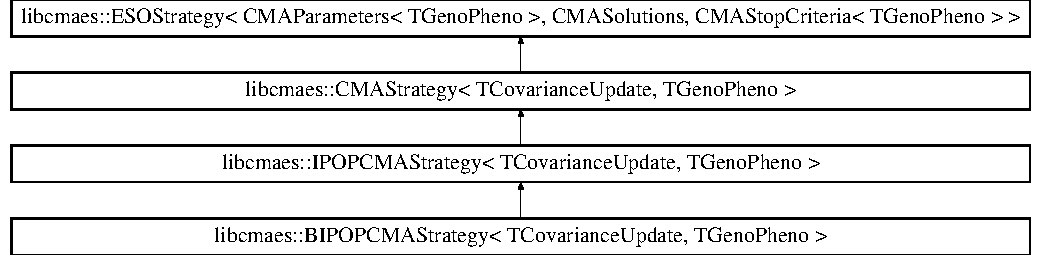
\includegraphics[height=3.430321cm]{classlibcmaes_1_1IPOPCMAStrategy}
\end{center}
\end{figure}
\subsection*{Public Member Functions}
\begin{DoxyCompactItemize}
\item 
\hyperlink{classlibcmaes_1_1IPOPCMAStrategy_a0fad3e1160695878d2d8075a4cddf786}{I\+P\+O\+P\+C\+M\+A\+Strategy} (Fit\+Func \&func, \hyperlink{classlibcmaes_1_1CMAParameters}{C\+M\+A\+Parameters}$<$ T\+Geno\+Pheno $>$ \&parameters)
\begin{DoxyCompactList}\small\item\em constructor. \end{DoxyCompactList}\item 
\hyperlink{classlibcmaes_1_1IPOPCMAStrategy_aa904db73802865f6a83d3ad05710bc67}{I\+P\+O\+P\+C\+M\+A\+Strategy} (Fit\+Func \&func, \hyperlink{classlibcmaes_1_1CMAParameters}{C\+M\+A\+Parameters}$<$ T\+Geno\+Pheno $>$ \&parameters, const \hyperlink{classlibcmaes_1_1CMASolutions}{C\+M\+A\+Solutions} \&solutions)
\begin{DoxyCompactList}\small\item\em constructor. \end{DoxyCompactList}\item 
\hypertarget{classlibcmaes_1_1IPOPCMAStrategy_a9b3b59e7caf752f48b37500d84736137}{void \hyperlink{classlibcmaes_1_1IPOPCMAStrategy_a9b3b59e7caf752f48b37500d84736137}{tell} ()}\label{classlibcmaes_1_1IPOPCMAStrategy_a9b3b59e7caf752f48b37500d84736137}

\begin{DoxyCompactList}\small\item\em Updates the covariance matrix and prepares for the next iteration. \end{DoxyCompactList}\item 
int \hyperlink{classlibcmaes_1_1IPOPCMAStrategy_a50555839c736d8189704d5d6d8e87553}{optimize} (const Eval\+Func \&evalf, const Ask\+Func \&askf, const Tell\+Func \&tellf)
\begin{DoxyCompactList}\small\item\em Finds the minimum of the objective function. It makes alternate calls to \hyperlink{classlibcmaes_1_1CMAStrategy_ab7266bc50732458ffcab690bc26380e6}{ask()}, \hyperlink{classlibcmaes_1_1IPOPCMAStrategy_a9b3b59e7caf752f48b37500d84736137}{tell()} and \hyperlink{classlibcmaes_1_1CMAStrategy_adc87b9c500959c800b6bc93d89432ecc}{stop()} until one of the termination criteria triggers. \end{DoxyCompactList}\item 
int \hyperlink{classlibcmaes_1_1IPOPCMAStrategy_a9c4f8ae0a8cbf600ba8fe7270e63172a}{optimize} ()
\begin{DoxyCompactList}\small\item\em Finds the minimum of the objective function. It makes alternate calls to \hyperlink{classlibcmaes_1_1CMAStrategy_ab7266bc50732458ffcab690bc26380e6}{ask()}, \hyperlink{classlibcmaes_1_1IPOPCMAStrategy_a9b3b59e7caf752f48b37500d84736137}{tell()} and \hyperlink{classlibcmaes_1_1CMAStrategy_adc87b9c500959c800b6bc93d89432ecc}{stop()} until one of the termination criteria triggers. \end{DoxyCompactList}\end{DoxyCompactItemize}
\subsection*{Protected Member Functions}
\begin{DoxyCompactItemize}
\item 
\hypertarget{classlibcmaes_1_1IPOPCMAStrategy_a210bde295a32c8da7906729831fcf5e2}{void {\bfseries lambda\+\_\+inc} ()}\label{classlibcmaes_1_1IPOPCMAStrategy_a210bde295a32c8da7906729831fcf5e2}

\item 
\hypertarget{classlibcmaes_1_1IPOPCMAStrategy_a8de562ec27e295c3b2517b1669fef0be}{void {\bfseries reset\+\_\+search\+\_\+state} ()}\label{classlibcmaes_1_1IPOPCMAStrategy_a8de562ec27e295c3b2517b1669fef0be}

\item 
\hypertarget{classlibcmaes_1_1IPOPCMAStrategy_a2f4d09dc1a86de8e4a1116cce4e518e8}{void {\bfseries capture\+\_\+best\+\_\+solution} (\hyperlink{classlibcmaes_1_1CMASolutions}{C\+M\+A\+Solutions} \&best\+\_\+run)}\label{classlibcmaes_1_1IPOPCMAStrategy_a2f4d09dc1a86de8e4a1116cce4e518e8}

\end{DoxyCompactItemize}
\subsection*{Additional Inherited Members}


\subsection{Detailed Description}
\subsubsection*{template$<$class T\+Covariance\+Update, class T\+Geno\+Pheno$>$class libcmaes\+::\+I\+P\+O\+P\+C\+M\+A\+Strategy$<$ T\+Covariance\+Update, T\+Geno\+Pheno $>$}

Implementation of the I\+P\+O\+P flavor of C\+M\+A-\/\+E\+S, with restarts that linearly increase the population of offsprings used in the update of the distribution parameters. 

\subsection{Constructor \& Destructor Documentation}
\hypertarget{classlibcmaes_1_1IPOPCMAStrategy_a0fad3e1160695878d2d8075a4cddf786}{\index{libcmaes\+::\+I\+P\+O\+P\+C\+M\+A\+Strategy@{libcmaes\+::\+I\+P\+O\+P\+C\+M\+A\+Strategy}!I\+P\+O\+P\+C\+M\+A\+Strategy@{I\+P\+O\+P\+C\+M\+A\+Strategy}}
\index{I\+P\+O\+P\+C\+M\+A\+Strategy@{I\+P\+O\+P\+C\+M\+A\+Strategy}!libcmaes\+::\+I\+P\+O\+P\+C\+M\+A\+Strategy@{libcmaes\+::\+I\+P\+O\+P\+C\+M\+A\+Strategy}}
\subsubsection[{I\+P\+O\+P\+C\+M\+A\+Strategy}]{\setlength{\rightskip}{0pt plus 5cm}template$<$class T\+Covariance\+Update , class T\+Geno\+Pheno $>$ {\bf libcmaes\+::\+I\+P\+O\+P\+C\+M\+A\+Strategy}$<$ T\+Covariance\+Update, T\+Geno\+Pheno $>$\+::{\bf I\+P\+O\+P\+C\+M\+A\+Strategy} (
\begin{DoxyParamCaption}
\item[{Fit\+Func \&}]{func, }
\item[{{\bf C\+M\+A\+Parameters}$<$ T\+Geno\+Pheno $>$ \&}]{parameters}
\end{DoxyParamCaption}
)}}\label{classlibcmaes_1_1IPOPCMAStrategy_a0fad3e1160695878d2d8075a4cddf786}


constructor. 


\begin{DoxyParams}{Parameters}
{\em func} & objective function to minimize \\
\hline
{\em parameters} & stochastic search parameters \\
\hline
\end{DoxyParams}
\hypertarget{classlibcmaes_1_1IPOPCMAStrategy_aa904db73802865f6a83d3ad05710bc67}{\index{libcmaes\+::\+I\+P\+O\+P\+C\+M\+A\+Strategy@{libcmaes\+::\+I\+P\+O\+P\+C\+M\+A\+Strategy}!I\+P\+O\+P\+C\+M\+A\+Strategy@{I\+P\+O\+P\+C\+M\+A\+Strategy}}
\index{I\+P\+O\+P\+C\+M\+A\+Strategy@{I\+P\+O\+P\+C\+M\+A\+Strategy}!libcmaes\+::\+I\+P\+O\+P\+C\+M\+A\+Strategy@{libcmaes\+::\+I\+P\+O\+P\+C\+M\+A\+Strategy}}
\subsubsection[{I\+P\+O\+P\+C\+M\+A\+Strategy}]{\setlength{\rightskip}{0pt plus 5cm}template$<$class T\+Covariance\+Update , class T\+Geno\+Pheno $>$ {\bf libcmaes\+::\+I\+P\+O\+P\+C\+M\+A\+Strategy}$<$ T\+Covariance\+Update, T\+Geno\+Pheno $>$\+::{\bf I\+P\+O\+P\+C\+M\+A\+Strategy} (
\begin{DoxyParamCaption}
\item[{Fit\+Func \&}]{func, }
\item[{{\bf C\+M\+A\+Parameters}$<$ T\+Geno\+Pheno $>$ \&}]{parameters, }
\item[{const {\bf C\+M\+A\+Solutions} \&}]{solutions}
\end{DoxyParamCaption}
)}}\label{classlibcmaes_1_1IPOPCMAStrategy_aa904db73802865f6a83d3ad05710bc67}


constructor. 


\begin{DoxyParams}{Parameters}
{\em func} & objective function to minimize \\
\hline
{\em parameters} & stochastic search parameters \\
\hline
{\em solutions} & solution to start search from \\
\hline
\end{DoxyParams}


\subsection{Member Function Documentation}
\hypertarget{classlibcmaes_1_1IPOPCMAStrategy_a50555839c736d8189704d5d6d8e87553}{\index{libcmaes\+::\+I\+P\+O\+P\+C\+M\+A\+Strategy@{libcmaes\+::\+I\+P\+O\+P\+C\+M\+A\+Strategy}!optimize@{optimize}}
\index{optimize@{optimize}!libcmaes\+::\+I\+P\+O\+P\+C\+M\+A\+Strategy@{libcmaes\+::\+I\+P\+O\+P\+C\+M\+A\+Strategy}}
\subsubsection[{optimize}]{\setlength{\rightskip}{0pt plus 5cm}template$<$class T\+Covariance\+Update , class T\+Geno\+Pheno $>$ int {\bf libcmaes\+::\+I\+P\+O\+P\+C\+M\+A\+Strategy}$<$ T\+Covariance\+Update, T\+Geno\+Pheno $>$\+::optimize (
\begin{DoxyParamCaption}
\item[{const Eval\+Func \&}]{evalf, }
\item[{const Ask\+Func \&}]{askf, }
\item[{const Tell\+Func \&}]{tellf}
\end{DoxyParamCaption}
)}}\label{classlibcmaes_1_1IPOPCMAStrategy_a50555839c736d8189704d5d6d8e87553}


Finds the minimum of the objective function. It makes alternate calls to \hyperlink{classlibcmaes_1_1CMAStrategy_ab7266bc50732458ffcab690bc26380e6}{ask()}, \hyperlink{classlibcmaes_1_1IPOPCMAStrategy_a9b3b59e7caf752f48b37500d84736137}{tell()} and \hyperlink{classlibcmaes_1_1CMAStrategy_adc87b9c500959c800b6bc93d89432ecc}{stop()} until one of the termination criteria triggers. 


\begin{DoxyParams}{Parameters}
{\em evalf} & custom eval function \\
\hline
{\em askf} & custom ask function \\
\hline
{\em tellf} & custom tell function \\
\hline
\end{DoxyParams}
\begin{DoxyReturn}{Returns}
success or error code, as defined in \hyperlink{opti__err_8h_source}{opti\+\_\+err.\+h} Note\+: the termination criteria code is held by \+\_\+solutions.\+\_\+run\+\_\+status 
\end{DoxyReturn}
\hypertarget{classlibcmaes_1_1IPOPCMAStrategy_a9c4f8ae0a8cbf600ba8fe7270e63172a}{\index{libcmaes\+::\+I\+P\+O\+P\+C\+M\+A\+Strategy@{libcmaes\+::\+I\+P\+O\+P\+C\+M\+A\+Strategy}!optimize@{optimize}}
\index{optimize@{optimize}!libcmaes\+::\+I\+P\+O\+P\+C\+M\+A\+Strategy@{libcmaes\+::\+I\+P\+O\+P\+C\+M\+A\+Strategy}}
\subsubsection[{optimize}]{\setlength{\rightskip}{0pt plus 5cm}template$<$class T\+Covariance\+Update , class T\+Geno\+Pheno $>$ int {\bf libcmaes\+::\+I\+P\+O\+P\+C\+M\+A\+Strategy}$<$ T\+Covariance\+Update, T\+Geno\+Pheno $>$\+::optimize (
\begin{DoxyParamCaption}
{}
\end{DoxyParamCaption}
)\hspace{0.3cm}{\ttfamily [inline]}}}\label{classlibcmaes_1_1IPOPCMAStrategy_a9c4f8ae0a8cbf600ba8fe7270e63172a}


Finds the minimum of the objective function. It makes alternate calls to \hyperlink{classlibcmaes_1_1CMAStrategy_ab7266bc50732458ffcab690bc26380e6}{ask()}, \hyperlink{classlibcmaes_1_1IPOPCMAStrategy_a9b3b59e7caf752f48b37500d84736137}{tell()} and \hyperlink{classlibcmaes_1_1CMAStrategy_adc87b9c500959c800b6bc93d89432ecc}{stop()} until one of the termination criteria triggers. 

\begin{DoxyReturn}{Returns}
success or error code, as defined in \hyperlink{opti__err_8h_source}{opti\+\_\+err.\+h} Note\+: the termination criteria code is held by \+\_\+solutions.\+\_\+run\+\_\+status 
\end{DoxyReturn}


The documentation for this class was generated from the following files\+:\begin{DoxyCompactItemize}
\item 
src/ipopcmastrategy.\+h\item 
src/ipopcmastrategy.\+cc\end{DoxyCompactItemize}

\hypertarget{structlastEvalStruct}{\section{last\-Eval\-Struct Struct Reference}
\label{structlastEvalStruct}\index{last\-Eval\-Struct@{last\-Eval\-Struct}}
}
\subsection*{Public Attributes}
\begin{DoxyCompactItemize}
\item 
\hypertarget{structlastEvalStruct_af5d431dd701c9bde0f8ad17b6506b2a3}{double {\bfseries num}}\label{structlastEvalStruct_af5d431dd701c9bde0f8ad17b6506b2a3}

\item 
\hypertarget{structlastEvalStruct_a83d6911bc9e5d20dc0eb02efd2bbc8d4}{double {\bfseries F}}\label{structlastEvalStruct_a83d6911bc9e5d20dc0eb02efd2bbc8d4}

\item 
\hypertarget{structlastEvalStruct_a22eb9ca20e6bc5a1f9da1b1daf0d81b3}{double {\bfseries Fnoisy}}\label{structlastEvalStruct_a22eb9ca20e6bc5a1f9da1b1daf0d81b3}

\item 
\hypertarget{structlastEvalStruct_aeefddf8f3a9a0c45f9cf4592338591d9}{double {\bfseries best\-Fnoisy}}\label{structlastEvalStruct_aeefddf8f3a9a0c45f9cf4592338591d9}

\item 
\hypertarget{structlastEvalStruct_a4de4d9e0b5854b52e1c03c935fcf19ed}{double {\bfseries x} \mbox{[}D\-I\-M\-\_\-\-M\-A\-X\mbox{]}}\label{structlastEvalStruct_a4de4d9e0b5854b52e1c03c935fcf19ed}

\item 
\hypertarget{structlastEvalStruct_a7fccf05ddaf98c80df3175f388900746}{int {\bfseries is\-Written}}\label{structlastEvalStruct_a7fccf05ddaf98c80df3175f388900746}

\end{DoxyCompactItemize}


The documentation for this struct was generated from the following file\-:\begin{DoxyCompactItemize}
\item 
tests/bbob.\-v13.\-09/c/bbob\-Structures.\-h\end{DoxyCompactItemize}

\hypertarget{classlibcmaes_1_1linScalingStrategy}{\section{libcmaes\-:\-:lin\-Scaling\-Strategy Class Reference}
\label{classlibcmaes_1_1linScalingStrategy}\index{libcmaes\-::lin\-Scaling\-Strategy@{libcmaes\-::lin\-Scaling\-Strategy}}
}
\subsection*{Public Member Functions}
\begin{DoxyCompactItemize}
\item 
\hypertarget{classlibcmaes_1_1linScalingStrategy_a02a64849f458cf8a440501d9e041b3e9}{{\bfseries lin\-Scaling\-Strategy} (const double $\ast$lbounds, const double $\ast$ubounds, const int \&dim)}\label{classlibcmaes_1_1linScalingStrategy_a02a64849f458cf8a440501d9e041b3e9}

\item 
\hypertarget{classlibcmaes_1_1linScalingStrategy_af798cb677f9f0ede111252c1ee05ab08}{{\bfseries lin\-Scaling\-Strategy} (const d\-Vec \&scaling, const d\-Vec \&shift)}\label{classlibcmaes_1_1linScalingStrategy_af798cb677f9f0ede111252c1ee05ab08}

\item 
\hypertarget{classlibcmaes_1_1linScalingStrategy_a043e908a7f3a7864c6a21ff5f041c48d}{void {\bfseries compute\-\_\-scaling} (const double $\ast$lbounds, const double $\ast$ubounds, const int \&dim)}\label{classlibcmaes_1_1linScalingStrategy_a043e908a7f3a7864c6a21ff5f041c48d}

\item 
\hypertarget{classlibcmaes_1_1linScalingStrategy_a6b111ef2e0f78c0f6a2cde92df7aa90e}{void {\bfseries scale\-\_\-to\-\_\-internal} (d\-Vec \&x, const d\-Vec \&y) const }\label{classlibcmaes_1_1linScalingStrategy_a6b111ef2e0f78c0f6a2cde92df7aa90e}

\item 
\hypertarget{classlibcmaes_1_1linScalingStrategy_a9ea06cf4d10c3015a154c763f88b862b}{void {\bfseries scale\-\_\-to\-\_\-f} (const d\-Vec \&x, d\-Vec \&y) const }\label{classlibcmaes_1_1linScalingStrategy_a9ea06cf4d10c3015a154c763f88b862b}

\end{DoxyCompactItemize}
\subsection*{Public Attributes}
\begin{DoxyCompactItemize}
\item 
double \hyperlink{classlibcmaes_1_1linScalingStrategy_ab5cf302d085ee302ed180a4c29c25bf2}{\-\_\-intmin} = 0.\-0
\item 
double \hyperlink{classlibcmaes_1_1linScalingStrategy_a8d25d3fd0d901c010e925cf786b78d04}{\-\_\-intmax} = 10.\-0
\item 
\hypertarget{classlibcmaes_1_1linScalingStrategy_a483cfaf8bceb634977c9cfd4683766b5}{d\-Vec {\bfseries \-\_\-scaling}}\label{classlibcmaes_1_1linScalingStrategy_a483cfaf8bceb634977c9cfd4683766b5}

\item 
\hypertarget{classlibcmaes_1_1linScalingStrategy_a42023d6a68d1efecb1d8ec3bc6261a9b}{d\-Vec {\bfseries \-\_\-shift}}\label{classlibcmaes_1_1linScalingStrategy_a42023d6a68d1efecb1d8ec3bc6261a9b}

\item 
\hypertarget{classlibcmaes_1_1linScalingStrategy_a61536bec2c52d4649663bb76e82af1b9}{bool {\bfseries \-\_\-id} = true}\label{classlibcmaes_1_1linScalingStrategy_a61536bec2c52d4649663bb76e82af1b9}

\end{DoxyCompactItemize}


\subsection{Member Data Documentation}
\hypertarget{classlibcmaes_1_1linScalingStrategy_a8d25d3fd0d901c010e925cf786b78d04}{\index{libcmaes\-::lin\-Scaling\-Strategy@{libcmaes\-::lin\-Scaling\-Strategy}!\-\_\-intmax@{\-\_\-intmax}}
\index{\-\_\-intmax@{\-\_\-intmax}!libcmaes::linScalingStrategy@{libcmaes\-::lin\-Scaling\-Strategy}}
\subsubsection[{\-\_\-intmax}]{\setlength{\rightskip}{0pt plus 5cm}double libcmaes\-::lin\-Scaling\-Strategy\-::\-\_\-intmax = 10.\-0}}\label{classlibcmaes_1_1linScalingStrategy_a8d25d3fd0d901c010e925cf786b78d04}
default internal max bound. \hypertarget{classlibcmaes_1_1linScalingStrategy_ab5cf302d085ee302ed180a4c29c25bf2}{\index{libcmaes\-::lin\-Scaling\-Strategy@{libcmaes\-::lin\-Scaling\-Strategy}!\-\_\-intmin@{\-\_\-intmin}}
\index{\-\_\-intmin@{\-\_\-intmin}!libcmaes::linScalingStrategy@{libcmaes\-::lin\-Scaling\-Strategy}}
\subsubsection[{\-\_\-intmin}]{\setlength{\rightskip}{0pt plus 5cm}double libcmaes\-::lin\-Scaling\-Strategy\-::\-\_\-intmin = 0.\-0}}\label{classlibcmaes_1_1linScalingStrategy_ab5cf302d085ee302ed180a4c29c25bf2}
default internal min bound. 

The documentation for this class was generated from the following file\-:\begin{DoxyCompactItemize}
\item 
src/scaling.\-h\end{DoxyCompactItemize}

\hypertarget{classlibcmaes_1_1NoBoundStrategy}{\section{libcmaes\-:\-:No\-Bound\-Strategy Class Reference}
\label{classlibcmaes_1_1NoBoundStrategy}\index{libcmaes\-::\-No\-Bound\-Strategy@{libcmaes\-::\-No\-Bound\-Strategy}}
}
\subsection*{Public Member Functions}
\begin{DoxyCompactItemize}
\item 
\hypertarget{classlibcmaes_1_1NoBoundStrategy_a726bc7b1e9f5dbde5ad97757ed94e470}{{\bfseries No\-Bound\-Strategy} (const double $\ast$lbounds=nullptr, const double $\ast$ubounds=nullptr, const int dim=0)}\label{classlibcmaes_1_1NoBoundStrategy_a726bc7b1e9f5dbde5ad97757ed94e470}

\item 
\hypertarget{classlibcmaes_1_1NoBoundStrategy_a766c30a177076c46b89be463ce1f3062}{void {\bfseries to\-\_\-f\-\_\-representation} (const d\-Vec \&x, d\-Vec \&y) const }\label{classlibcmaes_1_1NoBoundStrategy_a766c30a177076c46b89be463ce1f3062}

\item 
\hypertarget{classlibcmaes_1_1NoBoundStrategy_a9f2fe5e1b64188118add2e8e00603ba3}{double {\bfseries get\-L\-Bound} (const int \&k) const }\label{classlibcmaes_1_1NoBoundStrategy_a9f2fe5e1b64188118add2e8e00603ba3}

\item 
\hypertarget{classlibcmaes_1_1NoBoundStrategy_a2a0a9467aeb6b57749cc73499bf40620}{double {\bfseries get\-U\-Bound} (const int \&k) const }\label{classlibcmaes_1_1NoBoundStrategy_a2a0a9467aeb6b57749cc73499bf40620}

\end{DoxyCompactItemize}


The documentation for this class was generated from the following file\-:\begin{DoxyCompactItemize}
\item 
src/noboundstrategy.\-h\end{DoxyCompactItemize}

\hypertarget{classlibcmaes_1_1NoScalingStrategy}{\section{libcmaes\-:\-:No\-Scaling\-Strategy Class Reference}
\label{classlibcmaes_1_1NoScalingStrategy}\index{libcmaes\-::\-No\-Scaling\-Strategy@{libcmaes\-::\-No\-Scaling\-Strategy}}
}
\subsection*{Public Member Functions}
\begin{DoxyCompactItemize}
\item 
\hypertarget{classlibcmaes_1_1NoScalingStrategy_afa32ee30796e0daa71dacf0b39a24038}{{\bfseries No\-Scaling\-Strategy} (const double $\ast$lbounds, const double $\ast$ubounds, const int \&dim)}\label{classlibcmaes_1_1NoScalingStrategy_afa32ee30796e0daa71dacf0b39a24038}

\item 
\hypertarget{classlibcmaes_1_1NoScalingStrategy_a2cec97ec77df54410a5218d0fa24913c}{void {\bfseries scale\-\_\-to\-\_\-internal} (d\-Vec \&x, const d\-Vec \&y) const }\label{classlibcmaes_1_1NoScalingStrategy_a2cec97ec77df54410a5218d0fa24913c}

\item 
\hypertarget{classlibcmaes_1_1NoScalingStrategy_ae7c21e6a62a97a9fe4426923440750fc}{void {\bfseries scale\-\_\-to\-\_\-f} (const d\-Vec \&x, d\-Vec \&y) const }\label{classlibcmaes_1_1NoScalingStrategy_ae7c21e6a62a97a9fe4426923440750fc}

\end{DoxyCompactItemize}
\subsection*{Friends}
\begin{DoxyCompactItemize}
\item 
\hypertarget{classlibcmaes_1_1NoScalingStrategy_a78b1b9910ebce544de9b54b998e77879}{class {\bfseries C\-M\-A\-Solutions}}\label{classlibcmaes_1_1NoScalingStrategy_a78b1b9910ebce544de9b54b998e77879}

\item 
\hypertarget{classlibcmaes_1_1NoScalingStrategy_a30b6df18a1c8899440f1ca1273b26bb9}{{\footnotesize template$<$class U , class V $>$ }\\class {\bfseries Geno\-Pheno}}\label{classlibcmaes_1_1NoScalingStrategy_a30b6df18a1c8899440f1ca1273b26bb9}

\end{DoxyCompactItemize}


The documentation for this class was generated from the following file\-:\begin{DoxyCompactItemize}
\item 
src/scaling.\-h\end{DoxyCompactItemize}

\hypertarget{classlibcmaes_1_1Parameters}{\section{libcmaes\+:\+:Parameters$<$ T\+Geno\+Pheno $>$ Class Template Reference}
\label{classlibcmaes_1_1Parameters}\index{libcmaes\+::\+Parameters$<$ T\+Geno\+Pheno $>$@{libcmaes\+::\+Parameters$<$ T\+Geno\+Pheno $>$}}
}


Generic class for Evolution Strategy parameters.  




{\ttfamily \#include $<$parameters.\+h$>$}

Inheritance diagram for libcmaes\+:\+:Parameters$<$ T\+Geno\+Pheno $>$\+:\begin{figure}[H]
\begin{center}
\leavevmode
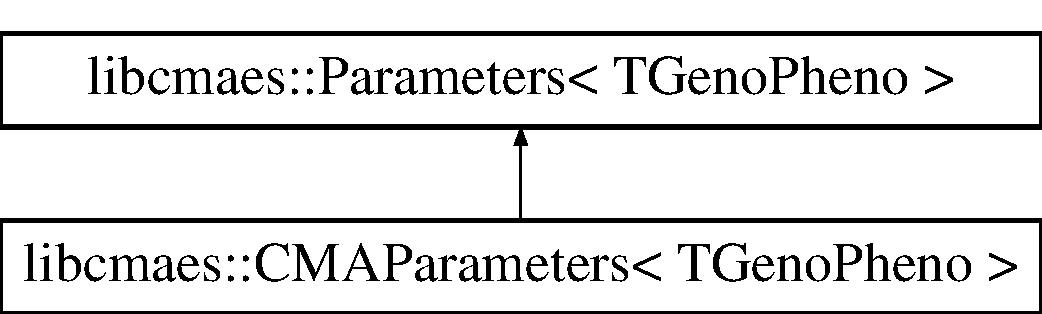
\includegraphics[height=2.000000cm]{classlibcmaes_1_1Parameters}
\end{center}
\end{figure}
\subsection*{Public Member Functions}
\begin{DoxyCompactItemize}
\item 
\hypertarget{classlibcmaes_1_1Parameters_a680f96c102aa0cb4c9e8d39b515392b9}{\hyperlink{classlibcmaes_1_1Parameters_a680f96c102aa0cb4c9e8d39b515392b9}{Parameters} ()}\label{classlibcmaes_1_1Parameters_a680f96c102aa0cb4c9e8d39b515392b9}

\begin{DoxyCompactList}\small\item\em empty constructor. \end{DoxyCompactList}\item 
\hyperlink{classlibcmaes_1_1Parameters_a082cedda8396793496e8d796bc0184b2}{Parameters} (const int \&\hyperlink{classlibcmaes_1_1Parameters_a95a3c04400a77d134bb1e9705189a24e}{dim}, const double $\ast$x0, const int \&\hyperlink{classlibcmaes_1_1Parameters_a3d569987e9a5eb61bc781ee75b2ab18a}{lambda}=-\/1, const uint64\+\_\+t \&seed=0, const T\+Geno\+Pheno \&gp=\hyperlink{classlibcmaes_1_1GenoPheno}{Geno\+Pheno}$<$ \hyperlink{classlibcmaes_1_1NoBoundStrategy}{No\+Bound\+Strategy} $>$())
\begin{DoxyCompactList}\small\item\em constructor \end{DoxyCompactList}\item 
void \hyperlink{classlibcmaes_1_1Parameters_a61660152146a78000b5cc59a0298a8f0}{set\+\_\+x0} (const double \&x0)
\begin{DoxyCompactList}\small\item\em sets initial objective function parameter values to x0 across all dimensions \end{DoxyCompactList}\item 
void \hyperlink{classlibcmaes_1_1Parameters_a50056ec90bc1b89295f8363eb566b8ce}{set\+\_\+x0} (const double $\ast$x0)
\begin{DoxyCompactList}\small\item\em sets initial objective function parameter values to array x0 \end{DoxyCompactList}\item 
void \hyperlink{classlibcmaes_1_1Parameters_a77985cc81f856083a63d85ebc11db0ae}{set\+\_\+x0} (const d\+Vec \&x0)
\begin{DoxyCompactList}\small\item\em sets initial objective function parameter values from \hyperlink{namespaceEigen}{Eigen} vector \end{DoxyCompactList}\item 
void \hyperlink{classlibcmaes_1_1Parameters_a2db4deff995719566b86bfc0c2df4e91}{set\+\_\+x0} (const double \&x0min, const double \&x0max)
\begin{DoxyCompactList}\small\item\em sets bounds on initial objective function parameter values. Bounds are the same across all dimensions, and initial value is sampled uniformly within these bounds. \end{DoxyCompactList}\item 
void \hyperlink{classlibcmaes_1_1Parameters_addda8e395450878e87538df7b4032cbe}{set\+\_\+x0} (const double $\ast$x0min, const double $\ast$x0max)
\begin{DoxyCompactList}\small\item\em sets bounds on initial objective function parameter values. Initial value is sampled uniformly within these bounds. \end{DoxyCompactList}\item 
void \hyperlink{classlibcmaes_1_1Parameters_ac3b37ba000eb460240554230f760039f}{set\+\_\+x0} (const std\+::vector$<$ double $>$ \&x0min, const std\+::vector$<$ double $>$ \&x0max)
\begin{DoxyCompactList}\small\item\em sets bounds on initial objective function parameter values. Initial value is sampled uniformly within these bounds. \end{DoxyCompactList}\item 
void \hyperlink{classlibcmaes_1_1Parameters_acc94e18faebb18dcaa0712a296e76949}{set\+\_\+x0} (const d\+Vec \&x0min, const d\+Vec \&x0max)
\begin{DoxyCompactList}\small\item\em sets bounds on initial objective function parameter values. Initial value is sampled uniformly within these bounds. \end{DoxyCompactList}\item 
d\+Vec \hyperlink{classlibcmaes_1_1Parameters_a1f7532a4bac9543094e7879baf3d73e1}{get\+\_\+x0min} () const 
\begin{DoxyCompactList}\small\item\em returns lower bound on x0 vector \end{DoxyCompactList}\item 
d\+Vec \hyperlink{classlibcmaes_1_1Parameters_adba08aae48f823c1611466ec86ae3b75}{get\+\_\+x0max} () const 
\begin{DoxyCompactList}\small\item\em returns upper bound on x0 vector \end{DoxyCompactList}\item 
void \hyperlink{classlibcmaes_1_1Parameters_a30236ca44b7de58b160bf2b1170f69b2}{set\+\_\+fixed\+\_\+p} (const int \&index, const double \&value)
\begin{DoxyCompactList}\small\item\em freezes a parameter to a given value during optimization. \end{DoxyCompactList}\item 
void \hyperlink{classlibcmaes_1_1Parameters_a540a57691845698e79af120f16d27f2c}{unset\+\_\+fixed\+\_\+p} (const int \&index)
\begin{DoxyCompactList}\small\item\em unfreezes a parameter. \end{DoxyCompactList}\item 
void \hyperlink{classlibcmaes_1_1Parameters_acefab965b50d45c6609e4f3267785ace}{set\+\_\+max\+\_\+iter} (const int \&maxiter)
\begin{DoxyCompactList}\small\item\em sets the maximum number of iterations allowed for the optimization. \end{DoxyCompactList}\item 
int \hyperlink{classlibcmaes_1_1Parameters_a95b8ff475b28b2cbf89cd147ab09eeee}{get\+\_\+max\+\_\+iter} () const 
\begin{DoxyCompactList}\small\item\em returns maximum number of iterations \end{DoxyCompactList}\item 
void \hyperlink{classlibcmaes_1_1Parameters_aa924cb4c8ffee0d148b63f5c0b55b4ce}{set\+\_\+max\+\_\+fevals} (const int \&fevals)
\begin{DoxyCompactList}\small\item\em sets the maximum budget of objective function calls allowed for the optimization. \end{DoxyCompactList}\item 
int \hyperlink{classlibcmaes_1_1Parameters_af738c73caee922feff43ba29218ea8ad}{get\+\_\+max\+\_\+fevals} () const 
\begin{DoxyCompactList}\small\item\em returns maximum budget of objective function calls \end{DoxyCompactList}\item 
void \hyperlink{classlibcmaes_1_1Parameters_a6ace7e5d230fcf82c70ba2dd3a801f97}{set\+\_\+ftarget} (const double \&val)
\begin{DoxyCompactList}\small\item\em sets the objective function target value when known. \end{DoxyCompactList}\item 
\hypertarget{classlibcmaes_1_1Parameters_aec14ab6c39a12e347080fa7e0f2e7c9f}{void \hyperlink{classlibcmaes_1_1Parameters_aec14ab6c39a12e347080fa7e0f2e7c9f}{reset\+\_\+ftarget} ()}\label{classlibcmaes_1_1Parameters_aec14ab6c39a12e347080fa7e0f2e7c9f}

\begin{DoxyCompactList}\small\item\em resets the objective function target value to its inactive state. \end{DoxyCompactList}\item 
double \hyperlink{classlibcmaes_1_1Parameters_ae7b39c351afbbb75a657ea5990899782}{get\+\_\+ftarget} () const 
\begin{DoxyCompactList}\small\item\em returns objective function target value. \end{DoxyCompactList}\item 
void \hyperlink{classlibcmaes_1_1Parameters_ac27d3bc99f554d771c24a1129ece2181}{set\+\_\+seed} (const int \&seed)
\begin{DoxyCompactList}\small\item\em sets random generator's seed, 0 is special value to generate random seed. \end{DoxyCompactList}\item 
int \hyperlink{classlibcmaes_1_1Parameters_af98c1effaa3e0a4321ae5046f1bdd615}{get\+\_\+seed} () const 
\begin{DoxyCompactList}\small\item\em returns random generator's seed. \end{DoxyCompactList}\item 
void \hyperlink{classlibcmaes_1_1Parameters_ad01dddcc81b121f20afeaafc09537304}{set\+\_\+ftolerance} (const double \&v)
\begin{DoxyCompactList}\small\item\em sets function tolerance as stopping criteria for Tol\+Hist\+Fun\+: monitors the difference in function value over iterations and stops optimization when below tolerance. \end{DoxyCompactList}\item 
double \hyperlink{classlibcmaes_1_1Parameters_a64b1867aa4d9aeb946e923d42452ff8d}{get\+\_\+ftolerance} () const 
\begin{DoxyCompactList}\small\item\em returns function tolerance \end{DoxyCompactList}\item 
void \hyperlink{classlibcmaes_1_1Parameters_aa131adbd299a29259034cac7cfe83009}{set\+\_\+xtolerance} (const double \&v)
\begin{DoxyCompactList}\small\item\em sets parameter tolerance as stopping criteria for Tol\+X. \end{DoxyCompactList}\item 
double \hyperlink{classlibcmaes_1_1Parameters_a75b95a875008a0216038d43369cd9171}{get\+\_\+xtolerance} () const 
\begin{DoxyCompactList}\small\item\em returns parameter tolerance \end{DoxyCompactList}\item 
int \hyperlink{classlibcmaes_1_1Parameters_a3d569987e9a5eb61bc781ee75b2ab18a}{lambda} () const 
\begin{DoxyCompactList}\small\item\em returns lambda, number of offsprings per generation \end{DoxyCompactList}\item 
int \hyperlink{classlibcmaes_1_1Parameters_a95a3c04400a77d134bb1e9705189a24e}{dim} () const 
\begin{DoxyCompactList}\small\item\em returns the problem's dimension \end{DoxyCompactList}\item 
void \hyperlink{classlibcmaes_1_1Parameters_ae93cf5c15dbe42b19339b26b1c57f872}{set\+\_\+quiet} (const bool \&\hyperlink{classlibcmaes_1_1Parameters_a8562a739088f9f9f466b8d658084c9f7}{quiet})
\begin{DoxyCompactList}\small\item\em sets the quiet mode (no output from the library) for the optimization at hand \end{DoxyCompactList}\item 
bool \hyperlink{classlibcmaes_1_1Parameters_a8562a739088f9f9f466b8d658084c9f7}{quiet} () const 
\begin{DoxyCompactList}\small\item\em returns whether the quiet mode is on. \end{DoxyCompactList}\item 
void \hyperlink{classlibcmaes_1_1Parameters_aeb869d18fa0c987f56216d9bfa1f1a0d}{set\+\_\+algo} (const int \&algo)
\begin{DoxyCompactList}\small\item\em sets the optimization algorithm. \end{DoxyCompactList}\item 
int \hyperlink{classlibcmaes_1_1Parameters_a39697cd6cfb705a970223f8e95894545}{get\+\_\+algo} () const 
\begin{DoxyCompactList}\small\item\em returns which algorithm is set for the optimization at hand. \end{DoxyCompactList}\item 
void \hyperlink{classlibcmaes_1_1Parameters_aeeab862124b864147e143bd86eb51cb5}{set\+\_\+gp} (const T\+Geno\+Pheno \&gp)
\begin{DoxyCompactList}\small\item\em sets the genotype/phenotype transform object. \end{DoxyCompactList}\item 
T\+Geno\+Pheno \hyperlink{classlibcmaes_1_1Parameters_a365039e6948ee2242c0ad34ed4ff02ab}{get\+\_\+gp} () const 
\begin{DoxyCompactList}\small\item\em returns the current genotype/phenotype transform object. \end{DoxyCompactList}\item 
void \hyperlink{classlibcmaes_1_1Parameters_ab96a2149ca63863d3f5618f54097df44}{set\+\_\+fplot} (const std\+::string \&fplot)
\begin{DoxyCompactList}\small\item\em sets the output filename (activates the output to file). \end{DoxyCompactList}\item 
void \hyperlink{classlibcmaes_1_1Parameters_a4d428eba994c5cdb7ab67729e4fdac6a}{set\+\_\+full\+\_\+fplot} (const bool \&b)
\begin{DoxyCompactList}\small\item\em activates / deactivates the full output (for legacy plotting). \end{DoxyCompactList}\item 
std\+::string \hyperlink{classlibcmaes_1_1Parameters_a6787bd16e95db6125a5e131ad58574cc}{get\+\_\+fplot} () const 
\begin{DoxyCompactList}\small\item\em returns the current output filename. \end{DoxyCompactList}\item 
void \hyperlink{classlibcmaes_1_1Parameters_a38082ad1568c356caff5b299d6faea11}{set\+\_\+gradient} (const bool \&gradient)
\begin{DoxyCompactList}\small\item\em activates the gradient injection scheme. If no gradient function is defined, injects a numerical gradient solution instead \end{DoxyCompactList}\item 
bool \hyperlink{classlibcmaes_1_1Parameters_ac7f6c27e00d1c0d744221b5a32e9efee}{get\+\_\+gradient} () const 
\begin{DoxyCompactList}\small\item\em returns whether the gradient injection scheme is activated. \end{DoxyCompactList}\item 
void \hyperlink{classlibcmaes_1_1Parameters_ac34068e69a36d06fed6599a7247bcb2e}{set\+\_\+edm} (const bool \&edm)
\begin{DoxyCompactList}\small\item\em activates computation of expected distance to minimum when optimization has completed \end{DoxyCompactList}\item 
bool \hyperlink{classlibcmaes_1_1Parameters_a3fa757be9e734622d77a831b3576aedb}{get\+\_\+edm} () const 
\begin{DoxyCompactList}\small\item\em returns whether edm is activated. \end{DoxyCompactList}\item 
void \hyperlink{classlibcmaes_1_1Parameters_a72995fb64587e6401d8b751343750c65}{set\+\_\+mt\+\_\+feval} (const bool \&mt)
\begin{DoxyCompactList}\small\item\em activate / deactivate the parallel evaluation of objective function \end{DoxyCompactList}\item 
bool \hyperlink{classlibcmaes_1_1Parameters_aac3914b24de6312e6d1fe3d493bb42f5}{get\+\_\+mt\+\_\+feval} () const 
\begin{DoxyCompactList}\small\item\em returns whether the parallel evaluation of objective function is activated \end{DoxyCompactList}\item 
void \hyperlink{classlibcmaes_1_1Parameters_a1226eeecac97019c183a9a85185efcc8}{set\+\_\+max\+\_\+hist} (const int \&m)
\begin{DoxyCompactList}\small\item\em sets maximum history size, allows to keep memory requirements fixed. \end{DoxyCompactList}\item 
void \hyperlink{classlibcmaes_1_1Parameters_a676f84fbe8726abf5ce88e117b159867}{set\+\_\+maximize} (const bool \&maximize)
\begin{DoxyCompactList}\small\item\em active internal maximization scheme (simply returns -\/f instead of f) \end{DoxyCompactList}\item 
bool \hyperlink{classlibcmaes_1_1Parameters_afec66b0ca5465b81498189e2cc8a14dc}{get\+\_\+maximize} () const 
\begin{DoxyCompactList}\small\item\em returns whether the maximization mode is enabled \end{DoxyCompactList}\item 
void \hyperlink{classlibcmaes_1_1Parameters_af8317ae69be35fdcb2c22c3848b3353f}{set\+\_\+initial\+\_\+fvalue} (const bool \&b)
\begin{DoxyCompactList}\small\item\em whether to compute initial objective function value (i.\+e. at x0) \end{DoxyCompactList}\item 
void \hyperlink{classlibcmaes_1_1Parameters_a40d2b4a06a716a858fc76127c49c66b3}{set\+\_\+uh} (const bool \&b)
\begin{DoxyCompactList}\small\item\em activates / deactivates uncertainty handling scheme. \end{DoxyCompactList}\item 
bool \hyperlink{classlibcmaes_1_1Parameters_a26dbffa26e99e17d7b0dc31bdca23bb2}{get\+\_\+uh} () const 
\begin{DoxyCompactList}\small\item\em get uncertainty handling status. \end{DoxyCompactList}\item 
void \hyperlink{classlibcmaes_1_1Parameters_abdf33ca4024935a04cd4081c411dac85}{set\+\_\+tpa} (const int \&b)
\begin{DoxyCompactList}\small\item\em activates / deactivates two-\/point adaptation step-\/size mechanism \end{DoxyCompactList}\item 
int \hyperlink{classlibcmaes_1_1Parameters_a72622c74df063f5d0f79f674559463e2}{get\+\_\+tpa} () const 
\begin{DoxyCompactList}\small\item\em get two-\/point adapation step-\/size mechanism status. \end{DoxyCompactList}\end{DoxyCompactItemize}
\subsection*{Protected Attributes}
\begin{DoxyCompactItemize}
\item 
int \hyperlink{classlibcmaes_1_1Parameters_affc62ae5c5f1db4f88e4c2dc96387af6}{\+\_\+dim}
\item 
int \hyperlink{classlibcmaes_1_1Parameters_af732f7206f23cbd6ec2bbd4e217a9a2b}{\+\_\+lambda} = -\/1
\item 
int \hyperlink{classlibcmaes_1_1Parameters_a60abfc730c5aa46e42ebd1598b59caa6}{\+\_\+max\+\_\+iter} = -\/1
\item 
int \hyperlink{classlibcmaes_1_1Parameters_ad316488121bd51f62b28e8183d591c9e}{\+\_\+max\+\_\+fevals} = -\/1
\item 
bool \hyperlink{classlibcmaes_1_1Parameters_a6f6dad55c02a23891e3280cad288295a}{\+\_\+quiet} = true
\item 
std\+::string \hyperlink{classlibcmaes_1_1Parameters_aa49511ea00199348ea94f1aa53fe5bc1}{\+\_\+fplot} = \char`\"{}\char`\"{}
\item 
bool \hyperlink{classlibcmaes_1_1Parameters_a00e08bf1e0de66bd07a1a4d0eb7c925f}{\+\_\+full\+\_\+fplot} = false
\item 
d\+Vec \hyperlink{classlibcmaes_1_1Parameters_aa3bb27467698d9cb7fc7e0a83b48800f}{\+\_\+x0min}
\item 
d\+Vec \hyperlink{classlibcmaes_1_1Parameters_aece9694af9bee78bb13b0994db7ac45e}{\+\_\+x0max}
\item 
double \hyperlink{classlibcmaes_1_1Parameters_a837dbcfba351a043441076a11666f92c}{\+\_\+ftarget} = -\/std\+::numeric\+\_\+limits$<$double$>$\+::infinity()
\item 
double \hyperlink{classlibcmaes_1_1Parameters_ab6c11cc112b5709e9039967e881c808e}{\+\_\+ftolerance} = 1e-\/12
\item 
double \hyperlink{classlibcmaes_1_1Parameters_aaa9e8eedba7d7140d116163b40f653f8}{\+\_\+xtol} = 1e-\/12
\item 
uint64\+\_\+t \hyperlink{classlibcmaes_1_1Parameters_ac6d616c3d5295fec8a0b230592fb767a}{\+\_\+seed} = 0
\item 
int \hyperlink{classlibcmaes_1_1Parameters_a7a5fc681b0c7294ef050ace344f923db}{\+\_\+algo} = 0
\item 
bool \hyperlink{classlibcmaes_1_1Parameters_aff76cebbfef51c20398aab8f49a3676a}{\+\_\+with\+\_\+gradient} =false
\item 
bool \hyperlink{classlibcmaes_1_1Parameters_adbaa11317ae66061e097c372522b8758}{\+\_\+with\+\_\+edm} =false
\item 
std\+::unordered\+\_\+map$<$ int, double $>$ \hyperlink{classlibcmaes_1_1Parameters_a83fdae9d4bb9b77c8ad955c6aac75086}{\+\_\+fixed\+\_\+p}
\item 
T\+Geno\+Pheno \hyperlink{classlibcmaes_1_1Parameters_ab8e153b4785de9358599caa840b94ef2}{\+\_\+gp}
\item 
bool \hyperlink{classlibcmaes_1_1Parameters_a78a3b97b4119776b661c1be4fc283069}{\+\_\+mt\+\_\+feval} = false
\item 
int \hyperlink{classlibcmaes_1_1Parameters_a6ecc091e7e10b30c067f28e5be05faff}{\+\_\+max\+\_\+hist} = -\/1
\item 
bool \hyperlink{classlibcmaes_1_1Parameters_a8c65760fc2d97303d9881c2a945d1d7b}{\+\_\+maximize} = false
\item 
bool \hyperlink{classlibcmaes_1_1Parameters_a421b56efbe82da078cbe32a6c59ea80f}{\+\_\+initial\+\_\+fvalue} = false
\item 
bool \hyperlink{classlibcmaes_1_1Parameters_a4dc4905889ab02a2a74386875dc4f834}{\+\_\+uh} = false
\item 
double \hyperlink{classlibcmaes_1_1Parameters_a35486ec0b31b3450a0cb10e54f16b7fd}{\+\_\+rlambda}
\item 
double \hyperlink{classlibcmaes_1_1Parameters_ab79e42306610b24fafe017a011373bd8}{\+\_\+epsuh} = 1e-\/7
\item 
double \hyperlink{classlibcmaes_1_1Parameters_af125dad682b5a40f05ac42351f548ff9}{\+\_\+thetauh} = 0.\+2
\item 
double \hyperlink{classlibcmaes_1_1Parameters_acedc12aaa2bcb0923279a15fc2fd4295}{\+\_\+csuh} = 1.\+0
\item 
double \hyperlink{classlibcmaes_1_1Parameters_afe9928f77d0413fb75a24fe0cb0f947b}{\+\_\+alphathuh} = 1.\+0
\item 
int \hyperlink{classlibcmaes_1_1Parameters_a9f38bf1e37112abf71045225817cd30b}{\+\_\+tpa} = 1
\item 
\hypertarget{classlibcmaes_1_1Parameters_ae1175ebd72ba7af46a3b7d8081e4a205}{double {\bfseries \+\_\+tpa\+\_\+csigma} = 0.\+3}\label{classlibcmaes_1_1Parameters_ae1175ebd72ba7af46a3b7d8081e4a205}

\end{DoxyCompactItemize}
\subsection*{Static Protected Attributes}
\begin{DoxyCompactItemize}
\item 
static std\+::map$<$ std\+::string, int $>$ \hyperlink{classlibcmaes_1_1Parameters_a5d2fd0ca871efd0f4f4b223515544204}{\+\_\+algos} = \{\{\char`\"{}cmaes\char`\"{},0\},\{\char`\"{}ipop\char`\"{},1\},\{\char`\"{}bipop\char`\"{},2\},\{\char`\"{}acmaes\char`\"{},3\},\{\char`\"{}aipop\char`\"{},4\},\{\char`\"{}abipop\char`\"{},5\},\{\char`\"{}sepcmaes\char`\"{},6\},\{\char`\"{}sepipop\char`\"{},7\},\{\char`\"{}sepbipop\char`\"{},8\},\{\char`\"{}sepacmaes\char`\"{},9\},\{\char`\"{}sepipop\char`\"{},10\},\{\char`\"{}sepbipop\char`\"{},11\},\{\char`\"{}vdcma\char`\"{},12\},\{\char`\"{}vdipopcma\char`\"{},13\},\{\char`\"{}vdbipopcma\char`\"{},14\}\}
\end{DoxyCompactItemize}
\subsection*{Friends}
\begin{DoxyCompactItemize}
\item 
\hypertarget{classlibcmaes_1_1Parameters_a78b1b9910ebce544de9b54b998e77879}{class {\bfseries C\+M\+A\+Solutions}}\label{classlibcmaes_1_1Parameters_a78b1b9910ebce544de9b54b998e77879}

\item 
\hypertarget{classlibcmaes_1_1Parameters_a07488b7628d12135de0243eb796e53a9}{{\footnotesize template$<$class U , class V $>$ }\\class {\bfseries C\+M\+A\+Strategy}}\label{classlibcmaes_1_1Parameters_a07488b7628d12135de0243eb796e53a9}

\item 
\hypertarget{classlibcmaes_1_1Parameters_ad6ebfad69a17421ae398d90c542aea13}{{\footnotesize template$<$class U , class V , class W $>$ }\\class {\bfseries E\+S\+O\+Strategy}}\label{classlibcmaes_1_1Parameters_ad6ebfad69a17421ae398d90c542aea13}

\item 
\hypertarget{classlibcmaes_1_1Parameters_aff56187b22ef0b3164ed7711dc0c82c3}{{\footnotesize template$<$class U $>$ }\\class {\bfseries C\+M\+A\+Stop\+Criteria}}\label{classlibcmaes_1_1Parameters_aff56187b22ef0b3164ed7711dc0c82c3}

\item 
\hypertarget{classlibcmaes_1_1Parameters_a083272459c67810fd3e8b1702c7d67c2}{{\footnotesize template$<$class U , class V $>$ }\\class {\bfseries I\+P\+O\+P\+C\+M\+A\+Strategy}}\label{classlibcmaes_1_1Parameters_a083272459c67810fd3e8b1702c7d67c2}

\item 
\hypertarget{classlibcmaes_1_1Parameters_ae97315b6fb514c42e8c3973f362ef2a2}{{\footnotesize template$<$class U , class V $>$ }\\class {\bfseries B\+I\+P\+O\+P\+C\+M\+A\+Strategy}}\label{classlibcmaes_1_1Parameters_ae97315b6fb514c42e8c3973f362ef2a2}

\item 
\hypertarget{classlibcmaes_1_1Parameters_aa62543a4caa6d6b288bb58ca5411539c}{class {\bfseries Covariance\+Update}}\label{classlibcmaes_1_1Parameters_aa62543a4caa6d6b288bb58ca5411539c}

\item 
\hypertarget{classlibcmaes_1_1Parameters_a81af003765a6521a192e5a37612c2fb5}{class {\bfseries A\+Covariance\+Update}}\label{classlibcmaes_1_1Parameters_a81af003765a6521a192e5a37612c2fb5}

\item 
\hypertarget{classlibcmaes_1_1Parameters_a867bde5f83097a4db1f667a3911efbae}{{\footnotesize template$<$class U $>$ }\\class {\bfseries errstats}}\label{classlibcmaes_1_1Parameters_a867bde5f83097a4db1f667a3911efbae}

\item 
\hypertarget{classlibcmaes_1_1Parameters_a3fceefe6a1e378ff9fef5d97117e5f47}{class {\bfseries V\+D\+C\+M\+A\+Update}}\label{classlibcmaes_1_1Parameters_a3fceefe6a1e378ff9fef5d97117e5f47}

\item 
\hypertarget{classlibcmaes_1_1Parameters_afb3142edf2def9ad64b319487505f2eb}{class {\bfseries Candidate}}\label{classlibcmaes_1_1Parameters_afb3142edf2def9ad64b319487505f2eb}

\end{DoxyCompactItemize}


\subsection{Detailed Description}
\subsubsection*{template$<$class T\+Geno\+Pheno = Geno\+Pheno$<$\+No\+Bound\+Strategy$>$$>$class libcmaes\+::\+Parameters$<$ T\+Geno\+Pheno $>$}

Generic class for Evolution Strategy parameters. 

\subsection{Constructor \& Destructor Documentation}
\hypertarget{classlibcmaes_1_1Parameters_a082cedda8396793496e8d796bc0184b2}{\index{libcmaes\+::\+Parameters@{libcmaes\+::\+Parameters}!Parameters@{Parameters}}
\index{Parameters@{Parameters}!libcmaes\+::\+Parameters@{libcmaes\+::\+Parameters}}
\subsubsection[{Parameters}]{\setlength{\rightskip}{0pt plus 5cm}template$<$class T\+Geno\+Pheno = Geno\+Pheno$<$\+No\+Bound\+Strategy$>$$>$ {\bf libcmaes\+::\+Parameters}$<$ T\+Geno\+Pheno $>$\+::{\bf Parameters} (
\begin{DoxyParamCaption}
\item[{const int \&}]{dim, }
\item[{const double $\ast$}]{x0, }
\item[{const int \&}]{lambda = {\ttfamily -\/1}, }
\item[{const uint64\+\_\+t \&}]{seed = {\ttfamily 0}, }
\item[{const T\+Geno\+Pheno \&}]{gp = {\ttfamily {\bf Geno\+Pheno}$<${\bf No\+Bound\+Strategy}$>$()}}
\end{DoxyParamCaption}
)\hspace{0.3cm}{\ttfamily [inline]}}}\label{classlibcmaes_1_1Parameters_a082cedda8396793496e8d796bc0184b2}


constructor 


\begin{DoxyParams}{Parameters}
{\em dim} & problem dimensions \\
\hline
{\em x0} & initial search point \\
\hline
{\em lambda} & number of offsprings sampled at each step \\
\hline
{\em seed} & initial random seed, useful for reproducing results (if unspecified, automatically generated from current time) \\
\hline
{\em gp} & genotype / phenotype object \\
\hline
\end{DoxyParams}


\subsection{Member Function Documentation}
\hypertarget{classlibcmaes_1_1Parameters_a95a3c04400a77d134bb1e9705189a24e}{\index{libcmaes\+::\+Parameters@{libcmaes\+::\+Parameters}!dim@{dim}}
\index{dim@{dim}!libcmaes\+::\+Parameters@{libcmaes\+::\+Parameters}}
\subsubsection[{dim}]{\setlength{\rightskip}{0pt plus 5cm}template$<$class T\+Geno\+Pheno = Geno\+Pheno$<$\+No\+Bound\+Strategy$>$$>$ int {\bf libcmaes\+::\+Parameters}$<$ T\+Geno\+Pheno $>$\+::dim (
\begin{DoxyParamCaption}
{}
\end{DoxyParamCaption}
) const\hspace{0.3cm}{\ttfamily [inline]}}}\label{classlibcmaes_1_1Parameters_a95a3c04400a77d134bb1e9705189a24e}


returns the problem's dimension 

\begin{DoxyReturn}{Returns}
dimensions 
\end{DoxyReturn}
\hypertarget{classlibcmaes_1_1Parameters_a39697cd6cfb705a970223f8e95894545}{\index{libcmaes\+::\+Parameters@{libcmaes\+::\+Parameters}!get\+\_\+algo@{get\+\_\+algo}}
\index{get\+\_\+algo@{get\+\_\+algo}!libcmaes\+::\+Parameters@{libcmaes\+::\+Parameters}}
\subsubsection[{get\+\_\+algo}]{\setlength{\rightskip}{0pt plus 5cm}template$<$class T\+Geno\+Pheno = Geno\+Pheno$<$\+No\+Bound\+Strategy$>$$>$ int {\bf libcmaes\+::\+Parameters}$<$ T\+Geno\+Pheno $>$\+::get\+\_\+algo (
\begin{DoxyParamCaption}
{}
\end{DoxyParamCaption}
) const\hspace{0.3cm}{\ttfamily [inline]}}}\label{classlibcmaes_1_1Parameters_a39697cd6cfb705a970223f8e95894545}


returns which algorithm is set for the optimization at hand. 

\begin{DoxyReturn}{Returns}
algorithm integer code 
\end{DoxyReturn}
\hypertarget{classlibcmaes_1_1Parameters_a3fa757be9e734622d77a831b3576aedb}{\index{libcmaes\+::\+Parameters@{libcmaes\+::\+Parameters}!get\+\_\+edm@{get\+\_\+edm}}
\index{get\+\_\+edm@{get\+\_\+edm}!libcmaes\+::\+Parameters@{libcmaes\+::\+Parameters}}
\subsubsection[{get\+\_\+edm}]{\setlength{\rightskip}{0pt plus 5cm}template$<$class T\+Geno\+Pheno = Geno\+Pheno$<$\+No\+Bound\+Strategy$>$$>$ bool {\bf libcmaes\+::\+Parameters}$<$ T\+Geno\+Pheno $>$\+::get\+\_\+edm (
\begin{DoxyParamCaption}
{}
\end{DoxyParamCaption}
) const\hspace{0.3cm}{\ttfamily [inline]}}}\label{classlibcmaes_1_1Parameters_a3fa757be9e734622d77a831b3576aedb}


returns whether edm is activated. 

\begin{DoxyReturn}{Returns}
edm 
\end{DoxyReturn}
\hypertarget{classlibcmaes_1_1Parameters_a6787bd16e95db6125a5e131ad58574cc}{\index{libcmaes\+::\+Parameters@{libcmaes\+::\+Parameters}!get\+\_\+fplot@{get\+\_\+fplot}}
\index{get\+\_\+fplot@{get\+\_\+fplot}!libcmaes\+::\+Parameters@{libcmaes\+::\+Parameters}}
\subsubsection[{get\+\_\+fplot}]{\setlength{\rightskip}{0pt plus 5cm}template$<$class T\+Geno\+Pheno = Geno\+Pheno$<$\+No\+Bound\+Strategy$>$$>$ std\+::string {\bf libcmaes\+::\+Parameters}$<$ T\+Geno\+Pheno $>$\+::get\+\_\+fplot (
\begin{DoxyParamCaption}
{}
\end{DoxyParamCaption}
) const\hspace{0.3cm}{\ttfamily [inline]}}}\label{classlibcmaes_1_1Parameters_a6787bd16e95db6125a5e131ad58574cc}


returns the current output filename. 

\begin{DoxyReturn}{Returns}
output filename 
\end{DoxyReturn}
\hypertarget{classlibcmaes_1_1Parameters_ae7b39c351afbbb75a657ea5990899782}{\index{libcmaes\+::\+Parameters@{libcmaes\+::\+Parameters}!get\+\_\+ftarget@{get\+\_\+ftarget}}
\index{get\+\_\+ftarget@{get\+\_\+ftarget}!libcmaes\+::\+Parameters@{libcmaes\+::\+Parameters}}
\subsubsection[{get\+\_\+ftarget}]{\setlength{\rightskip}{0pt plus 5cm}template$<$class T\+Geno\+Pheno = Geno\+Pheno$<$\+No\+Bound\+Strategy$>$$>$ double {\bf libcmaes\+::\+Parameters}$<$ T\+Geno\+Pheno $>$\+::get\+\_\+ftarget (
\begin{DoxyParamCaption}
{}
\end{DoxyParamCaption}
) const\hspace{0.3cm}{\ttfamily [inline]}}}\label{classlibcmaes_1_1Parameters_ae7b39c351afbbb75a657ea5990899782}


returns objective function target value. 

\begin{DoxyReturn}{Returns}
objective function target value 
\end{DoxyReturn}
\hypertarget{classlibcmaes_1_1Parameters_a64b1867aa4d9aeb946e923d42452ff8d}{\index{libcmaes\+::\+Parameters@{libcmaes\+::\+Parameters}!get\+\_\+ftolerance@{get\+\_\+ftolerance}}
\index{get\+\_\+ftolerance@{get\+\_\+ftolerance}!libcmaes\+::\+Parameters@{libcmaes\+::\+Parameters}}
\subsubsection[{get\+\_\+ftolerance}]{\setlength{\rightskip}{0pt plus 5cm}template$<$class T\+Geno\+Pheno = Geno\+Pheno$<$\+No\+Bound\+Strategy$>$$>$ double {\bf libcmaes\+::\+Parameters}$<$ T\+Geno\+Pheno $>$\+::get\+\_\+ftolerance (
\begin{DoxyParamCaption}
{}
\end{DoxyParamCaption}
) const\hspace{0.3cm}{\ttfamily [inline]}}}\label{classlibcmaes_1_1Parameters_a64b1867aa4d9aeb946e923d42452ff8d}


returns function tolerance 

\begin{DoxyReturn}{Returns}
function tolerance 
\end{DoxyReturn}
\hypertarget{classlibcmaes_1_1Parameters_a365039e6948ee2242c0ad34ed4ff02ab}{\index{libcmaes\+::\+Parameters@{libcmaes\+::\+Parameters}!get\+\_\+gp@{get\+\_\+gp}}
\index{get\+\_\+gp@{get\+\_\+gp}!libcmaes\+::\+Parameters@{libcmaes\+::\+Parameters}}
\subsubsection[{get\+\_\+gp}]{\setlength{\rightskip}{0pt plus 5cm}template$<$class T\+Geno\+Pheno = Geno\+Pheno$<$\+No\+Bound\+Strategy$>$$>$ T\+Geno\+Pheno {\bf libcmaes\+::\+Parameters}$<$ T\+Geno\+Pheno $>$\+::get\+\_\+gp (
\begin{DoxyParamCaption}
{}
\end{DoxyParamCaption}
) const\hspace{0.3cm}{\ttfamily [inline]}}}\label{classlibcmaes_1_1Parameters_a365039e6948ee2242c0ad34ed4ff02ab}


returns the current genotype/phenotype transform object. 

\begin{DoxyReturn}{Returns}
\hyperlink{classlibcmaes_1_1GenoPheno}{Geno\+Pheno} object 
\end{DoxyReturn}
\hypertarget{classlibcmaes_1_1Parameters_ac7f6c27e00d1c0d744221b5a32e9efee}{\index{libcmaes\+::\+Parameters@{libcmaes\+::\+Parameters}!get\+\_\+gradient@{get\+\_\+gradient}}
\index{get\+\_\+gradient@{get\+\_\+gradient}!libcmaes\+::\+Parameters@{libcmaes\+::\+Parameters}}
\subsubsection[{get\+\_\+gradient}]{\setlength{\rightskip}{0pt plus 5cm}template$<$class T\+Geno\+Pheno = Geno\+Pheno$<$\+No\+Bound\+Strategy$>$$>$ bool {\bf libcmaes\+::\+Parameters}$<$ T\+Geno\+Pheno $>$\+::get\+\_\+gradient (
\begin{DoxyParamCaption}
{}
\end{DoxyParamCaption}
) const\hspace{0.3cm}{\ttfamily [inline]}}}\label{classlibcmaes_1_1Parameters_ac7f6c27e00d1c0d744221b5a32e9efee}


returns whether the gradient injection scheme is activated. 

\begin{DoxyReturn}{Returns}
with gradient 
\end{DoxyReturn}
\hypertarget{classlibcmaes_1_1Parameters_af738c73caee922feff43ba29218ea8ad}{\index{libcmaes\+::\+Parameters@{libcmaes\+::\+Parameters}!get\+\_\+max\+\_\+fevals@{get\+\_\+max\+\_\+fevals}}
\index{get\+\_\+max\+\_\+fevals@{get\+\_\+max\+\_\+fevals}!libcmaes\+::\+Parameters@{libcmaes\+::\+Parameters}}
\subsubsection[{get\+\_\+max\+\_\+fevals}]{\setlength{\rightskip}{0pt plus 5cm}template$<$class T\+Geno\+Pheno = Geno\+Pheno$<$\+No\+Bound\+Strategy$>$$>$ int {\bf libcmaes\+::\+Parameters}$<$ T\+Geno\+Pheno $>$\+::get\+\_\+max\+\_\+fevals (
\begin{DoxyParamCaption}
{}
\end{DoxyParamCaption}
) const\hspace{0.3cm}{\ttfamily [inline]}}}\label{classlibcmaes_1_1Parameters_af738c73caee922feff43ba29218ea8ad}


returns maximum budget of objective function calls 

\begin{DoxyReturn}{Returns}
max number of objective function evaluations 
\end{DoxyReturn}
\hypertarget{classlibcmaes_1_1Parameters_a95b8ff475b28b2cbf89cd147ab09eeee}{\index{libcmaes\+::\+Parameters@{libcmaes\+::\+Parameters}!get\+\_\+max\+\_\+iter@{get\+\_\+max\+\_\+iter}}
\index{get\+\_\+max\+\_\+iter@{get\+\_\+max\+\_\+iter}!libcmaes\+::\+Parameters@{libcmaes\+::\+Parameters}}
\subsubsection[{get\+\_\+max\+\_\+iter}]{\setlength{\rightskip}{0pt plus 5cm}template$<$class T\+Geno\+Pheno = Geno\+Pheno$<$\+No\+Bound\+Strategy$>$$>$ int {\bf libcmaes\+::\+Parameters}$<$ T\+Geno\+Pheno $>$\+::get\+\_\+max\+\_\+iter (
\begin{DoxyParamCaption}
{}
\end{DoxyParamCaption}
) const\hspace{0.3cm}{\ttfamily [inline]}}}\label{classlibcmaes_1_1Parameters_a95b8ff475b28b2cbf89cd147ab09eeee}


returns maximum number of iterations 

\begin{DoxyReturn}{Returns}
max number of iterations allowed 
\end{DoxyReturn}
\hypertarget{classlibcmaes_1_1Parameters_afec66b0ca5465b81498189e2cc8a14dc}{\index{libcmaes\+::\+Parameters@{libcmaes\+::\+Parameters}!get\+\_\+maximize@{get\+\_\+maximize}}
\index{get\+\_\+maximize@{get\+\_\+maximize}!libcmaes\+::\+Parameters@{libcmaes\+::\+Parameters}}
\subsubsection[{get\+\_\+maximize}]{\setlength{\rightskip}{0pt plus 5cm}template$<$class T\+Geno\+Pheno = Geno\+Pheno$<$\+No\+Bound\+Strategy$>$$>$ bool {\bf libcmaes\+::\+Parameters}$<$ T\+Geno\+Pheno $>$\+::get\+\_\+maximize (
\begin{DoxyParamCaption}
{}
\end{DoxyParamCaption}
) const\hspace{0.3cm}{\ttfamily [inline]}}}\label{classlibcmaes_1_1Parameters_afec66b0ca5465b81498189e2cc8a14dc}


returns whether the maximization mode is enabled 

\begin{DoxyReturn}{Returns}
true if maximizing 
\end{DoxyReturn}
\hypertarget{classlibcmaes_1_1Parameters_aac3914b24de6312e6d1fe3d493bb42f5}{\index{libcmaes\+::\+Parameters@{libcmaes\+::\+Parameters}!get\+\_\+mt\+\_\+feval@{get\+\_\+mt\+\_\+feval}}
\index{get\+\_\+mt\+\_\+feval@{get\+\_\+mt\+\_\+feval}!libcmaes\+::\+Parameters@{libcmaes\+::\+Parameters}}
\subsubsection[{get\+\_\+mt\+\_\+feval}]{\setlength{\rightskip}{0pt plus 5cm}template$<$class T\+Geno\+Pheno = Geno\+Pheno$<$\+No\+Bound\+Strategy$>$$>$ bool {\bf libcmaes\+::\+Parameters}$<$ T\+Geno\+Pheno $>$\+::get\+\_\+mt\+\_\+feval (
\begin{DoxyParamCaption}
{}
\end{DoxyParamCaption}
) const\hspace{0.3cm}{\ttfamily [inline]}}}\label{classlibcmaes_1_1Parameters_aac3914b24de6312e6d1fe3d493bb42f5}


returns whether the parallel evaluation of objective function is activated 

\begin{DoxyReturn}{Returns}
activation status 
\end{DoxyReturn}
\hypertarget{classlibcmaes_1_1Parameters_af98c1effaa3e0a4321ae5046f1bdd615}{\index{libcmaes\+::\+Parameters@{libcmaes\+::\+Parameters}!get\+\_\+seed@{get\+\_\+seed}}
\index{get\+\_\+seed@{get\+\_\+seed}!libcmaes\+::\+Parameters@{libcmaes\+::\+Parameters}}
\subsubsection[{get\+\_\+seed}]{\setlength{\rightskip}{0pt plus 5cm}template$<$class T\+Geno\+Pheno = Geno\+Pheno$<$\+No\+Bound\+Strategy$>$$>$ int {\bf libcmaes\+::\+Parameters}$<$ T\+Geno\+Pheno $>$\+::get\+\_\+seed (
\begin{DoxyParamCaption}
{}
\end{DoxyParamCaption}
) const\hspace{0.3cm}{\ttfamily [inline]}}}\label{classlibcmaes_1_1Parameters_af98c1effaa3e0a4321ae5046f1bdd615}


returns random generator's seed. 

\begin{DoxyReturn}{Returns}
integer seed 
\end{DoxyReturn}
\hypertarget{classlibcmaes_1_1Parameters_a72622c74df063f5d0f79f674559463e2}{\index{libcmaes\+::\+Parameters@{libcmaes\+::\+Parameters}!get\+\_\+tpa@{get\+\_\+tpa}}
\index{get\+\_\+tpa@{get\+\_\+tpa}!libcmaes\+::\+Parameters@{libcmaes\+::\+Parameters}}
\subsubsection[{get\+\_\+tpa}]{\setlength{\rightskip}{0pt plus 5cm}template$<$class T\+Geno\+Pheno = Geno\+Pheno$<$\+No\+Bound\+Strategy$>$$>$ int {\bf libcmaes\+::\+Parameters}$<$ T\+Geno\+Pheno $>$\+::get\+\_\+tpa (
\begin{DoxyParamCaption}
{}
\end{DoxyParamCaption}
) const\hspace{0.3cm}{\ttfamily [inline]}}}\label{classlibcmaes_1_1Parameters_a72622c74df063f5d0f79f674559463e2}


get two-\/point adapation step-\/size mechanism status. 

\begin{DoxyReturn}{Returns}
two-\/point adaptation status. 
\end{DoxyReturn}
\hypertarget{classlibcmaes_1_1Parameters_a26dbffa26e99e17d7b0dc31bdca23bb2}{\index{libcmaes\+::\+Parameters@{libcmaes\+::\+Parameters}!get\+\_\+uh@{get\+\_\+uh}}
\index{get\+\_\+uh@{get\+\_\+uh}!libcmaes\+::\+Parameters@{libcmaes\+::\+Parameters}}
\subsubsection[{get\+\_\+uh}]{\setlength{\rightskip}{0pt plus 5cm}template$<$class T\+Geno\+Pheno = Geno\+Pheno$<$\+No\+Bound\+Strategy$>$$>$ bool {\bf libcmaes\+::\+Parameters}$<$ T\+Geno\+Pheno $>$\+::get\+\_\+uh (
\begin{DoxyParamCaption}
{}
\end{DoxyParamCaption}
) const\hspace{0.3cm}{\ttfamily [inline]}}}\label{classlibcmaes_1_1Parameters_a26dbffa26e99e17d7b0dc31bdca23bb2}


get uncertainty handling status. 

\begin{DoxyReturn}{Returns}
uncertainty handling status. 
\end{DoxyReturn}
\hypertarget{classlibcmaes_1_1Parameters_adba08aae48f823c1611466ec86ae3b75}{\index{libcmaes\+::\+Parameters@{libcmaes\+::\+Parameters}!get\+\_\+x0max@{get\+\_\+x0max}}
\index{get\+\_\+x0max@{get\+\_\+x0max}!libcmaes\+::\+Parameters@{libcmaes\+::\+Parameters}}
\subsubsection[{get\+\_\+x0max}]{\setlength{\rightskip}{0pt plus 5cm}template$<$class T\+Geno\+Pheno = Geno\+Pheno$<$\+No\+Bound\+Strategy$>$$>$ d\+Vec {\bf libcmaes\+::\+Parameters}$<$ T\+Geno\+Pheno $>$\+::get\+\_\+x0max (
\begin{DoxyParamCaption}
{}
\end{DoxyParamCaption}
) const\hspace{0.3cm}{\ttfamily [inline]}}}\label{classlibcmaes_1_1Parameters_adba08aae48f823c1611466ec86ae3b75}


returns upper bound on x0 vector 

\begin{DoxyReturn}{Returns}
upper bound on x0 
\end{DoxyReturn}
\hypertarget{classlibcmaes_1_1Parameters_a1f7532a4bac9543094e7879baf3d73e1}{\index{libcmaes\+::\+Parameters@{libcmaes\+::\+Parameters}!get\+\_\+x0min@{get\+\_\+x0min}}
\index{get\+\_\+x0min@{get\+\_\+x0min}!libcmaes\+::\+Parameters@{libcmaes\+::\+Parameters}}
\subsubsection[{get\+\_\+x0min}]{\setlength{\rightskip}{0pt plus 5cm}template$<$class T\+Geno\+Pheno = Geno\+Pheno$<$\+No\+Bound\+Strategy$>$$>$ d\+Vec {\bf libcmaes\+::\+Parameters}$<$ T\+Geno\+Pheno $>$\+::get\+\_\+x0min (
\begin{DoxyParamCaption}
{}
\end{DoxyParamCaption}
) const\hspace{0.3cm}{\ttfamily [inline]}}}\label{classlibcmaes_1_1Parameters_a1f7532a4bac9543094e7879baf3d73e1}


returns lower bound on x0 vector 

\begin{DoxyReturn}{Returns}
lower bound on x0 
\end{DoxyReturn}
\hypertarget{classlibcmaes_1_1Parameters_a75b95a875008a0216038d43369cd9171}{\index{libcmaes\+::\+Parameters@{libcmaes\+::\+Parameters}!get\+\_\+xtolerance@{get\+\_\+xtolerance}}
\index{get\+\_\+xtolerance@{get\+\_\+xtolerance}!libcmaes\+::\+Parameters@{libcmaes\+::\+Parameters}}
\subsubsection[{get\+\_\+xtolerance}]{\setlength{\rightskip}{0pt plus 5cm}template$<$class T\+Geno\+Pheno = Geno\+Pheno$<$\+No\+Bound\+Strategy$>$$>$ double {\bf libcmaes\+::\+Parameters}$<$ T\+Geno\+Pheno $>$\+::get\+\_\+xtolerance (
\begin{DoxyParamCaption}
{}
\end{DoxyParamCaption}
) const\hspace{0.3cm}{\ttfamily [inline]}}}\label{classlibcmaes_1_1Parameters_a75b95a875008a0216038d43369cd9171}


returns parameter tolerance 

\begin{DoxyReturn}{Returns}
parameter tolerance 
\end{DoxyReturn}
\hypertarget{classlibcmaes_1_1Parameters_a3d569987e9a5eb61bc781ee75b2ab18a}{\index{libcmaes\+::\+Parameters@{libcmaes\+::\+Parameters}!lambda@{lambda}}
\index{lambda@{lambda}!libcmaes\+::\+Parameters@{libcmaes\+::\+Parameters}}
\subsubsection[{lambda}]{\setlength{\rightskip}{0pt plus 5cm}template$<$class T\+Geno\+Pheno = Geno\+Pheno$<$\+No\+Bound\+Strategy$>$$>$ int {\bf libcmaes\+::\+Parameters}$<$ T\+Geno\+Pheno $>$\+::lambda (
\begin{DoxyParamCaption}
{}
\end{DoxyParamCaption}
) const\hspace{0.3cm}{\ttfamily [inline]}}}\label{classlibcmaes_1_1Parameters_a3d569987e9a5eb61bc781ee75b2ab18a}


returns lambda, number of offsprings per generation 

\begin{DoxyReturn}{Returns}
lambda 
\end{DoxyReturn}
\hypertarget{classlibcmaes_1_1Parameters_a8562a739088f9f9f466b8d658084c9f7}{\index{libcmaes\+::\+Parameters@{libcmaes\+::\+Parameters}!quiet@{quiet}}
\index{quiet@{quiet}!libcmaes\+::\+Parameters@{libcmaes\+::\+Parameters}}
\subsubsection[{quiet}]{\setlength{\rightskip}{0pt plus 5cm}template$<$class T\+Geno\+Pheno = Geno\+Pheno$<$\+No\+Bound\+Strategy$>$$>$ bool {\bf libcmaes\+::\+Parameters}$<$ T\+Geno\+Pheno $>$\+::quiet (
\begin{DoxyParamCaption}
{}
\end{DoxyParamCaption}
) const\hspace{0.3cm}{\ttfamily [inline]}}}\label{classlibcmaes_1_1Parameters_a8562a739088f9f9f466b8d658084c9f7}


returns whether the quiet mode is on. 

\begin{DoxyReturn}{Returns}
quiet mode 
\end{DoxyReturn}
\hypertarget{classlibcmaes_1_1Parameters_aeb869d18fa0c987f56216d9bfa1f1a0d}{\index{libcmaes\+::\+Parameters@{libcmaes\+::\+Parameters}!set\+\_\+algo@{set\+\_\+algo}}
\index{set\+\_\+algo@{set\+\_\+algo}!libcmaes\+::\+Parameters@{libcmaes\+::\+Parameters}}
\subsubsection[{set\+\_\+algo}]{\setlength{\rightskip}{0pt plus 5cm}template$<$class T\+Geno\+Pheno = Geno\+Pheno$<$\+No\+Bound\+Strategy$>$$>$ void {\bf libcmaes\+::\+Parameters}$<$ T\+Geno\+Pheno $>$\+::set\+\_\+algo (
\begin{DoxyParamCaption}
\item[{const int \&}]{algo}
\end{DoxyParamCaption}
)\hspace{0.3cm}{\ttfamily [inline]}}}\label{classlibcmaes_1_1Parameters_aeb869d18fa0c987f56216d9bfa1f1a0d}


sets the optimization algorithm. 


\begin{DoxyParams}{Parameters}
{\em algo} & from C\+M\+A\+E\+S\+\_\+\+D\+E\+F\+A\+U\+L\+T, I\+P\+O\+P\+\_\+\+C\+M\+A\+E\+S, B\+I\+P\+O\+P\+\_\+\+C\+M\+A\+E\+S, a\+C\+M\+A\+E\+S, a\+I\+P\+O\+P\+\_\+\+C\+M\+A\+E\+S, a\+B\+I\+P\+O\+P\+\_\+\+C\+M\+A\+E\+S, sep\+C\+M\+A\+E\+S, sep\+I\+P\+O\+P\+\_\+\+C\+M\+A\+E\+S, sep\+B\+I\+P\+O\+P\+\_\+\+C\+M\+A\+E\+S, sepa\+C\+M\+A\+E\+S, sepa\+I\+P\+O\+P\+\_\+\+C\+M\+A\+E\+S, sepa\+B\+I\+P\+O\+P\+\_\+\+C\+M\+A\+E\+S, V\+D\+\_\+\+C\+M\+A\+E\+S, V\+D\+\_\+\+I\+P\+O\+P\+\_\+\+C\+M\+A\+E\+S, V\+D\+\_\+\+B\+I\+P\+O\+P\+\_\+\+C\+M\+A\+E\+S \\
\hline
\end{DoxyParams}
\hypertarget{classlibcmaes_1_1Parameters_ac34068e69a36d06fed6599a7247bcb2e}{\index{libcmaes\+::\+Parameters@{libcmaes\+::\+Parameters}!set\+\_\+edm@{set\+\_\+edm}}
\index{set\+\_\+edm@{set\+\_\+edm}!libcmaes\+::\+Parameters@{libcmaes\+::\+Parameters}}
\subsubsection[{set\+\_\+edm}]{\setlength{\rightskip}{0pt plus 5cm}template$<$class T\+Geno\+Pheno = Geno\+Pheno$<$\+No\+Bound\+Strategy$>$$>$ void {\bf libcmaes\+::\+Parameters}$<$ T\+Geno\+Pheno $>$\+::set\+\_\+edm (
\begin{DoxyParamCaption}
\item[{const bool \&}]{edm}
\end{DoxyParamCaption}
)\hspace{0.3cm}{\ttfamily [inline]}}}\label{classlibcmaes_1_1Parameters_ac34068e69a36d06fed6599a7247bcb2e}


activates computation of expected distance to minimum when optimization has completed 


\begin{DoxyParams}{Parameters}
{\em edm} & true / false \\
\hline
\end{DoxyParams}
\hypertarget{classlibcmaes_1_1Parameters_a30236ca44b7de58b160bf2b1170f69b2}{\index{libcmaes\+::\+Parameters@{libcmaes\+::\+Parameters}!set\+\_\+fixed\+\_\+p@{set\+\_\+fixed\+\_\+p}}
\index{set\+\_\+fixed\+\_\+p@{set\+\_\+fixed\+\_\+p}!libcmaes\+::\+Parameters@{libcmaes\+::\+Parameters}}
\subsubsection[{set\+\_\+fixed\+\_\+p}]{\setlength{\rightskip}{0pt plus 5cm}template$<$class T\+Geno\+Pheno = Geno\+Pheno$<$\+No\+Bound\+Strategy$>$$>$ void {\bf libcmaes\+::\+Parameters}$<$ T\+Geno\+Pheno $>$\+::set\+\_\+fixed\+\_\+p (
\begin{DoxyParamCaption}
\item[{const int \&}]{index, }
\item[{const double \&}]{value}
\end{DoxyParamCaption}
)\hspace{0.3cm}{\ttfamily [inline]}}}\label{classlibcmaes_1_1Parameters_a30236ca44b7de58b160bf2b1170f69b2}


freezes a parameter to a given value during optimization. 


\begin{DoxyParams}{Parameters}
{\em index} & dimension index of the parameter to be frozen \\
\hline
{\em value} & frozen value of the parameter \\
\hline
\end{DoxyParams}
\hypertarget{classlibcmaes_1_1Parameters_ab96a2149ca63863d3f5618f54097df44}{\index{libcmaes\+::\+Parameters@{libcmaes\+::\+Parameters}!set\+\_\+fplot@{set\+\_\+fplot}}
\index{set\+\_\+fplot@{set\+\_\+fplot}!libcmaes\+::\+Parameters@{libcmaes\+::\+Parameters}}
\subsubsection[{set\+\_\+fplot}]{\setlength{\rightskip}{0pt plus 5cm}template$<$class T\+Geno\+Pheno = Geno\+Pheno$<$\+No\+Bound\+Strategy$>$$>$ void {\bf libcmaes\+::\+Parameters}$<$ T\+Geno\+Pheno $>$\+::set\+\_\+fplot (
\begin{DoxyParamCaption}
\item[{const std\+::string \&}]{fplot}
\end{DoxyParamCaption}
)\hspace{0.3cm}{\ttfamily [inline]}}}\label{classlibcmaes_1_1Parameters_ab96a2149ca63863d3f5618f54097df44}


sets the output filename (activates the output to file). 


\begin{DoxyParams}{Parameters}
{\em fplot} & filename \\
\hline
\end{DoxyParams}
\hypertarget{classlibcmaes_1_1Parameters_a6ace7e5d230fcf82c70ba2dd3a801f97}{\index{libcmaes\+::\+Parameters@{libcmaes\+::\+Parameters}!set\+\_\+ftarget@{set\+\_\+ftarget}}
\index{set\+\_\+ftarget@{set\+\_\+ftarget}!libcmaes\+::\+Parameters@{libcmaes\+::\+Parameters}}
\subsubsection[{set\+\_\+ftarget}]{\setlength{\rightskip}{0pt plus 5cm}template$<$class T\+Geno\+Pheno = Geno\+Pheno$<$\+No\+Bound\+Strategy$>$$>$ void {\bf libcmaes\+::\+Parameters}$<$ T\+Geno\+Pheno $>$\+::set\+\_\+ftarget (
\begin{DoxyParamCaption}
\item[{const double \&}]{val}
\end{DoxyParamCaption}
)\hspace{0.3cm}{\ttfamily [inline]}}}\label{classlibcmaes_1_1Parameters_a6ace7e5d230fcf82c70ba2dd3a801f97}


sets the objective function target value when known. 


\begin{DoxyParams}{Parameters}
{\em val} & objective function target value \\
\hline
\end{DoxyParams}
\hypertarget{classlibcmaes_1_1Parameters_ad01dddcc81b121f20afeaafc09537304}{\index{libcmaes\+::\+Parameters@{libcmaes\+::\+Parameters}!set\+\_\+ftolerance@{set\+\_\+ftolerance}}
\index{set\+\_\+ftolerance@{set\+\_\+ftolerance}!libcmaes\+::\+Parameters@{libcmaes\+::\+Parameters}}
\subsubsection[{set\+\_\+ftolerance}]{\setlength{\rightskip}{0pt plus 5cm}template$<$class T\+Geno\+Pheno = Geno\+Pheno$<$\+No\+Bound\+Strategy$>$$>$ void {\bf libcmaes\+::\+Parameters}$<$ T\+Geno\+Pheno $>$\+::set\+\_\+ftolerance (
\begin{DoxyParamCaption}
\item[{const double \&}]{v}
\end{DoxyParamCaption}
)\hspace{0.3cm}{\ttfamily [inline]}}}\label{classlibcmaes_1_1Parameters_ad01dddcc81b121f20afeaafc09537304}


sets function tolerance as stopping criteria for Tol\+Hist\+Fun\+: monitors the difference in function value over iterations and stops optimization when below tolerance. 


\begin{DoxyParams}{Parameters}
{\em v} & value of the function tolerance. \\
\hline
\end{DoxyParams}
\hypertarget{classlibcmaes_1_1Parameters_a4d428eba994c5cdb7ab67729e4fdac6a}{\index{libcmaes\+::\+Parameters@{libcmaes\+::\+Parameters}!set\+\_\+full\+\_\+fplot@{set\+\_\+full\+\_\+fplot}}
\index{set\+\_\+full\+\_\+fplot@{set\+\_\+full\+\_\+fplot}!libcmaes\+::\+Parameters@{libcmaes\+::\+Parameters}}
\subsubsection[{set\+\_\+full\+\_\+fplot}]{\setlength{\rightskip}{0pt plus 5cm}template$<$class T\+Geno\+Pheno = Geno\+Pheno$<$\+No\+Bound\+Strategy$>$$>$ void {\bf libcmaes\+::\+Parameters}$<$ T\+Geno\+Pheno $>$\+::set\+\_\+full\+\_\+fplot (
\begin{DoxyParamCaption}
\item[{const bool \&}]{b}
\end{DoxyParamCaption}
)\hspace{0.3cm}{\ttfamily [inline]}}}\label{classlibcmaes_1_1Parameters_a4d428eba994c5cdb7ab67729e4fdac6a}


activates / deactivates the full output (for legacy plotting). 


\begin{DoxyParams}{Parameters}
{\em b} & whether to activate / deactivate \\
\hline
\end{DoxyParams}
\hypertarget{classlibcmaes_1_1Parameters_aeeab862124b864147e143bd86eb51cb5}{\index{libcmaes\+::\+Parameters@{libcmaes\+::\+Parameters}!set\+\_\+gp@{set\+\_\+gp}}
\index{set\+\_\+gp@{set\+\_\+gp}!libcmaes\+::\+Parameters@{libcmaes\+::\+Parameters}}
\subsubsection[{set\+\_\+gp}]{\setlength{\rightskip}{0pt plus 5cm}template$<$class T\+Geno\+Pheno = Geno\+Pheno$<$\+No\+Bound\+Strategy$>$$>$ void {\bf libcmaes\+::\+Parameters}$<$ T\+Geno\+Pheno $>$\+::set\+\_\+gp (
\begin{DoxyParamCaption}
\item[{const T\+Geno\+Pheno \&}]{gp}
\end{DoxyParamCaption}
)\hspace{0.3cm}{\ttfamily [inline]}}}\label{classlibcmaes_1_1Parameters_aeeab862124b864147e143bd86eb51cb5}


sets the genotype/phenotype transform object. 


\begin{DoxyParams}{Parameters}
{\em gp} & \hyperlink{classlibcmaes_1_1GenoPheno}{Geno\+Pheno} object \\
\hline
\end{DoxyParams}
\hypertarget{classlibcmaes_1_1Parameters_a38082ad1568c356caff5b299d6faea11}{\index{libcmaes\+::\+Parameters@{libcmaes\+::\+Parameters}!set\+\_\+gradient@{set\+\_\+gradient}}
\index{set\+\_\+gradient@{set\+\_\+gradient}!libcmaes\+::\+Parameters@{libcmaes\+::\+Parameters}}
\subsubsection[{set\+\_\+gradient}]{\setlength{\rightskip}{0pt plus 5cm}template$<$class T\+Geno\+Pheno = Geno\+Pheno$<$\+No\+Bound\+Strategy$>$$>$ void {\bf libcmaes\+::\+Parameters}$<$ T\+Geno\+Pheno $>$\+::set\+\_\+gradient (
\begin{DoxyParamCaption}
\item[{const bool \&}]{gradient}
\end{DoxyParamCaption}
)\hspace{0.3cm}{\ttfamily [inline]}}}\label{classlibcmaes_1_1Parameters_a38082ad1568c356caff5b299d6faea11}


activates the gradient injection scheme. If no gradient function is defined, injects a numerical gradient solution instead 


\begin{DoxyParams}{Parameters}
{\em gradient} & true/false \\
\hline
\end{DoxyParams}
\hypertarget{classlibcmaes_1_1Parameters_af8317ae69be35fdcb2c22c3848b3353f}{\index{libcmaes\+::\+Parameters@{libcmaes\+::\+Parameters}!set\+\_\+initial\+\_\+fvalue@{set\+\_\+initial\+\_\+fvalue}}
\index{set\+\_\+initial\+\_\+fvalue@{set\+\_\+initial\+\_\+fvalue}!libcmaes\+::\+Parameters@{libcmaes\+::\+Parameters}}
\subsubsection[{set\+\_\+initial\+\_\+fvalue}]{\setlength{\rightskip}{0pt plus 5cm}template$<$class T\+Geno\+Pheno = Geno\+Pheno$<$\+No\+Bound\+Strategy$>$$>$ void {\bf libcmaes\+::\+Parameters}$<$ T\+Geno\+Pheno $>$\+::set\+\_\+initial\+\_\+fvalue (
\begin{DoxyParamCaption}
\item[{const bool \&}]{b}
\end{DoxyParamCaption}
)\hspace{0.3cm}{\ttfamily [inline]}}}\label{classlibcmaes_1_1Parameters_af8317ae69be35fdcb2c22c3848b3353f}


whether to compute initial objective function value (i.\+e. at x0) 


\begin{DoxyParams}{Parameters}
{\em b} & activates / deactivates \\
\hline
\end{DoxyParams}
\hypertarget{classlibcmaes_1_1Parameters_aa924cb4c8ffee0d148b63f5c0b55b4ce}{\index{libcmaes\+::\+Parameters@{libcmaes\+::\+Parameters}!set\+\_\+max\+\_\+fevals@{set\+\_\+max\+\_\+fevals}}
\index{set\+\_\+max\+\_\+fevals@{set\+\_\+max\+\_\+fevals}!libcmaes\+::\+Parameters@{libcmaes\+::\+Parameters}}
\subsubsection[{set\+\_\+max\+\_\+fevals}]{\setlength{\rightskip}{0pt plus 5cm}template$<$class T\+Geno\+Pheno = Geno\+Pheno$<$\+No\+Bound\+Strategy$>$$>$ void {\bf libcmaes\+::\+Parameters}$<$ T\+Geno\+Pheno $>$\+::set\+\_\+max\+\_\+fevals (
\begin{DoxyParamCaption}
\item[{const int \&}]{fevals}
\end{DoxyParamCaption}
)\hspace{0.3cm}{\ttfamily [inline]}}}\label{classlibcmaes_1_1Parameters_aa924cb4c8ffee0d148b63f5c0b55b4ce}


sets the maximum budget of objective function calls allowed for the optimization. 


\begin{DoxyParams}{Parameters}
{\em fevals} & maximum number of objective function evaluations \\
\hline
\end{DoxyParams}
\hypertarget{classlibcmaes_1_1Parameters_a1226eeecac97019c183a9a85185efcc8}{\index{libcmaes\+::\+Parameters@{libcmaes\+::\+Parameters}!set\+\_\+max\+\_\+hist@{set\+\_\+max\+\_\+hist}}
\index{set\+\_\+max\+\_\+hist@{set\+\_\+max\+\_\+hist}!libcmaes\+::\+Parameters@{libcmaes\+::\+Parameters}}
\subsubsection[{set\+\_\+max\+\_\+hist}]{\setlength{\rightskip}{0pt plus 5cm}template$<$class T\+Geno\+Pheno = Geno\+Pheno$<$\+No\+Bound\+Strategy$>$$>$ void {\bf libcmaes\+::\+Parameters}$<$ T\+Geno\+Pheno $>$\+::set\+\_\+max\+\_\+hist (
\begin{DoxyParamCaption}
\item[{const int \&}]{m}
\end{DoxyParamCaption}
)\hspace{0.3cm}{\ttfamily [inline]}}}\label{classlibcmaes_1_1Parameters_a1226eeecac97019c183a9a85185efcc8}


sets maximum history size, allows to keep memory requirements fixed. 


\begin{DoxyParams}{Parameters}
{\em m} & number of steps of candidate history that are kept into memory (for stopping criteria equalfunvals mostly). \\
\hline
\end{DoxyParams}
\hypertarget{classlibcmaes_1_1Parameters_acefab965b50d45c6609e4f3267785ace}{\index{libcmaes\+::\+Parameters@{libcmaes\+::\+Parameters}!set\+\_\+max\+\_\+iter@{set\+\_\+max\+\_\+iter}}
\index{set\+\_\+max\+\_\+iter@{set\+\_\+max\+\_\+iter}!libcmaes\+::\+Parameters@{libcmaes\+::\+Parameters}}
\subsubsection[{set\+\_\+max\+\_\+iter}]{\setlength{\rightskip}{0pt plus 5cm}template$<$class T\+Geno\+Pheno = Geno\+Pheno$<$\+No\+Bound\+Strategy$>$$>$ void {\bf libcmaes\+::\+Parameters}$<$ T\+Geno\+Pheno $>$\+::set\+\_\+max\+\_\+iter (
\begin{DoxyParamCaption}
\item[{const int \&}]{maxiter}
\end{DoxyParamCaption}
)\hspace{0.3cm}{\ttfamily [inline]}}}\label{classlibcmaes_1_1Parameters_acefab965b50d45c6609e4f3267785ace}


sets the maximum number of iterations allowed for the optimization. 


\begin{DoxyParams}{Parameters}
{\em maxiter} & maximum number of allowed iterations \\
\hline
\end{DoxyParams}
\hypertarget{classlibcmaes_1_1Parameters_a676f84fbe8726abf5ce88e117b159867}{\index{libcmaes\+::\+Parameters@{libcmaes\+::\+Parameters}!set\+\_\+maximize@{set\+\_\+maximize}}
\index{set\+\_\+maximize@{set\+\_\+maximize}!libcmaes\+::\+Parameters@{libcmaes\+::\+Parameters}}
\subsubsection[{set\+\_\+maximize}]{\setlength{\rightskip}{0pt plus 5cm}template$<$class T\+Geno\+Pheno = Geno\+Pheno$<$\+No\+Bound\+Strategy$>$$>$ void {\bf libcmaes\+::\+Parameters}$<$ T\+Geno\+Pheno $>$\+::set\+\_\+maximize (
\begin{DoxyParamCaption}
\item[{const bool \&}]{maximize}
\end{DoxyParamCaption}
)\hspace{0.3cm}{\ttfamily [inline]}}}\label{classlibcmaes_1_1Parameters_a676f84fbe8726abf5ce88e117b159867}


active internal maximization scheme (simply returns -\/f instead of f) 


\begin{DoxyParams}{Parameters}
{\em maximize} & whether to maximize instead of minimizing \\
\hline
\end{DoxyParams}
\hypertarget{classlibcmaes_1_1Parameters_a72995fb64587e6401d8b751343750c65}{\index{libcmaes\+::\+Parameters@{libcmaes\+::\+Parameters}!set\+\_\+mt\+\_\+feval@{set\+\_\+mt\+\_\+feval}}
\index{set\+\_\+mt\+\_\+feval@{set\+\_\+mt\+\_\+feval}!libcmaes\+::\+Parameters@{libcmaes\+::\+Parameters}}
\subsubsection[{set\+\_\+mt\+\_\+feval}]{\setlength{\rightskip}{0pt plus 5cm}template$<$class T\+Geno\+Pheno = Geno\+Pheno$<$\+No\+Bound\+Strategy$>$$>$ void {\bf libcmaes\+::\+Parameters}$<$ T\+Geno\+Pheno $>$\+::set\+\_\+mt\+\_\+feval (
\begin{DoxyParamCaption}
\item[{const bool \&}]{mt}
\end{DoxyParamCaption}
)\hspace{0.3cm}{\ttfamily [inline]}}}\label{classlibcmaes_1_1Parameters_a72995fb64587e6401d8b751343750c65}


activate / deactivate the parallel evaluation of objective function 


\begin{DoxyParams}{Parameters}
{\em mt} & true for activated, false otherwise \\
\hline
\end{DoxyParams}
\hypertarget{classlibcmaes_1_1Parameters_ae93cf5c15dbe42b19339b26b1c57f872}{\index{libcmaes\+::\+Parameters@{libcmaes\+::\+Parameters}!set\+\_\+quiet@{set\+\_\+quiet}}
\index{set\+\_\+quiet@{set\+\_\+quiet}!libcmaes\+::\+Parameters@{libcmaes\+::\+Parameters}}
\subsubsection[{set\+\_\+quiet}]{\setlength{\rightskip}{0pt plus 5cm}template$<$class T\+Geno\+Pheno = Geno\+Pheno$<$\+No\+Bound\+Strategy$>$$>$ void {\bf libcmaes\+::\+Parameters}$<$ T\+Geno\+Pheno $>$\+::set\+\_\+quiet (
\begin{DoxyParamCaption}
\item[{const bool \&}]{quiet}
\end{DoxyParamCaption}
)\hspace{0.3cm}{\ttfamily [inline]}}}\label{classlibcmaes_1_1Parameters_ae93cf5c15dbe42b19339b26b1c57f872}


sets the quiet mode (no output from the library) for the optimization at hand 


\begin{DoxyParams}{Parameters}
{\em quiet} & true / false \\
\hline
\end{DoxyParams}
\hypertarget{classlibcmaes_1_1Parameters_ac27d3bc99f554d771c24a1129ece2181}{\index{libcmaes\+::\+Parameters@{libcmaes\+::\+Parameters}!set\+\_\+seed@{set\+\_\+seed}}
\index{set\+\_\+seed@{set\+\_\+seed}!libcmaes\+::\+Parameters@{libcmaes\+::\+Parameters}}
\subsubsection[{set\+\_\+seed}]{\setlength{\rightskip}{0pt plus 5cm}template$<$class T\+Geno\+Pheno = Geno\+Pheno$<$\+No\+Bound\+Strategy$>$$>$ void {\bf libcmaes\+::\+Parameters}$<$ T\+Geno\+Pheno $>$\+::set\+\_\+seed (
\begin{DoxyParamCaption}
\item[{const int \&}]{seed}
\end{DoxyParamCaption}
)\hspace{0.3cm}{\ttfamily [inline]}}}\label{classlibcmaes_1_1Parameters_ac27d3bc99f554d771c24a1129ece2181}


sets random generator's seed, 0 is special value to generate random seed. 


\begin{DoxyParams}{Parameters}
{\em seed} & integer seed \\
\hline
\end{DoxyParams}
\hypertarget{classlibcmaes_1_1Parameters_abdf33ca4024935a04cd4081c411dac85}{\index{libcmaes\+::\+Parameters@{libcmaes\+::\+Parameters}!set\+\_\+tpa@{set\+\_\+tpa}}
\index{set\+\_\+tpa@{set\+\_\+tpa}!libcmaes\+::\+Parameters@{libcmaes\+::\+Parameters}}
\subsubsection[{set\+\_\+tpa}]{\setlength{\rightskip}{0pt plus 5cm}template$<$class T\+Geno\+Pheno = Geno\+Pheno$<$\+No\+Bound\+Strategy$>$$>$ void {\bf libcmaes\+::\+Parameters}$<$ T\+Geno\+Pheno $>$\+::set\+\_\+tpa (
\begin{DoxyParamCaption}
\item[{const int \&}]{b}
\end{DoxyParamCaption}
)\hspace{0.3cm}{\ttfamily [inline]}}}\label{classlibcmaes_1_1Parameters_abdf33ca4024935a04cd4081c411dac85}


activates / deactivates two-\/point adaptation step-\/size mechanism 


\begin{DoxyParams}{Parameters}
{\em b} & 0\+: no, 1\+: auto, 2\+: yes \\
\hline
\end{DoxyParams}
\hypertarget{classlibcmaes_1_1Parameters_a40d2b4a06a716a858fc76127c49c66b3}{\index{libcmaes\+::\+Parameters@{libcmaes\+::\+Parameters}!set\+\_\+uh@{set\+\_\+uh}}
\index{set\+\_\+uh@{set\+\_\+uh}!libcmaes\+::\+Parameters@{libcmaes\+::\+Parameters}}
\subsubsection[{set\+\_\+uh}]{\setlength{\rightskip}{0pt plus 5cm}template$<$class T\+Geno\+Pheno = Geno\+Pheno$<$\+No\+Bound\+Strategy$>$$>$ void {\bf libcmaes\+::\+Parameters}$<$ T\+Geno\+Pheno $>$\+::set\+\_\+uh (
\begin{DoxyParamCaption}
\item[{const bool \&}]{b}
\end{DoxyParamCaption}
)\hspace{0.3cm}{\ttfamily [inline]}}}\label{classlibcmaes_1_1Parameters_a40d2b4a06a716a858fc76127c49c66b3}


activates / deactivates uncertainty handling scheme. 


\begin{DoxyParams}{Parameters}
{\em b} & activates / deactivates \\
\hline
\end{DoxyParams}
\hypertarget{classlibcmaes_1_1Parameters_a61660152146a78000b5cc59a0298a8f0}{\index{libcmaes\+::\+Parameters@{libcmaes\+::\+Parameters}!set\+\_\+x0@{set\+\_\+x0}}
\index{set\+\_\+x0@{set\+\_\+x0}!libcmaes\+::\+Parameters@{libcmaes\+::\+Parameters}}
\subsubsection[{set\+\_\+x0}]{\setlength{\rightskip}{0pt plus 5cm}template$<$class T\+Geno\+Pheno = Geno\+Pheno$<$\+No\+Bound\+Strategy$>$$>$ void {\bf libcmaes\+::\+Parameters}$<$ T\+Geno\+Pheno $>$\+::set\+\_\+x0 (
\begin{DoxyParamCaption}
\item[{const double \&}]{x0}
\end{DoxyParamCaption}
)\hspace{0.3cm}{\ttfamily [inline]}}}\label{classlibcmaes_1_1Parameters_a61660152146a78000b5cc59a0298a8f0}


sets initial objective function parameter values to x0 across all dimensions 


\begin{DoxyParams}{Parameters}
{\em x0} & initial value \\
\hline
\end{DoxyParams}
\hypertarget{classlibcmaes_1_1Parameters_a50056ec90bc1b89295f8363eb566b8ce}{\index{libcmaes\+::\+Parameters@{libcmaes\+::\+Parameters}!set\+\_\+x0@{set\+\_\+x0}}
\index{set\+\_\+x0@{set\+\_\+x0}!libcmaes\+::\+Parameters@{libcmaes\+::\+Parameters}}
\subsubsection[{set\+\_\+x0}]{\setlength{\rightskip}{0pt plus 5cm}template$<$class T\+Geno\+Pheno = Geno\+Pheno$<$\+No\+Bound\+Strategy$>$$>$ void {\bf libcmaes\+::\+Parameters}$<$ T\+Geno\+Pheno $>$\+::set\+\_\+x0 (
\begin{DoxyParamCaption}
\item[{const double $\ast$}]{x0}
\end{DoxyParamCaption}
)\hspace{0.3cm}{\ttfamily [inline]}}}\label{classlibcmaes_1_1Parameters_a50056ec90bc1b89295f8363eb566b8ce}


sets initial objective function parameter values to array x0 


\begin{DoxyParams}{Parameters}
{\em x0} & array of initial parameter values \\
\hline
\end{DoxyParams}
\hypertarget{classlibcmaes_1_1Parameters_a77985cc81f856083a63d85ebc11db0ae}{\index{libcmaes\+::\+Parameters@{libcmaes\+::\+Parameters}!set\+\_\+x0@{set\+\_\+x0}}
\index{set\+\_\+x0@{set\+\_\+x0}!libcmaes\+::\+Parameters@{libcmaes\+::\+Parameters}}
\subsubsection[{set\+\_\+x0}]{\setlength{\rightskip}{0pt plus 5cm}template$<$class T\+Geno\+Pheno = Geno\+Pheno$<$\+No\+Bound\+Strategy$>$$>$ void {\bf libcmaes\+::\+Parameters}$<$ T\+Geno\+Pheno $>$\+::set\+\_\+x0 (
\begin{DoxyParamCaption}
\item[{const d\+Vec \&}]{x0}
\end{DoxyParamCaption}
)\hspace{0.3cm}{\ttfamily [inline]}}}\label{classlibcmaes_1_1Parameters_a77985cc81f856083a63d85ebc11db0ae}


sets initial objective function parameter values from \hyperlink{namespaceEigen}{Eigen} vector 


\begin{DoxyParams}{Parameters}
{\em x0} & \hyperlink{namespaceEigen}{Eigen} vector of initial parameter values \\
\hline
\end{DoxyParams}
\hypertarget{classlibcmaes_1_1Parameters_a2db4deff995719566b86bfc0c2df4e91}{\index{libcmaes\+::\+Parameters@{libcmaes\+::\+Parameters}!set\+\_\+x0@{set\+\_\+x0}}
\index{set\+\_\+x0@{set\+\_\+x0}!libcmaes\+::\+Parameters@{libcmaes\+::\+Parameters}}
\subsubsection[{set\+\_\+x0}]{\setlength{\rightskip}{0pt plus 5cm}template$<$class T\+Geno\+Pheno = Geno\+Pheno$<$\+No\+Bound\+Strategy$>$$>$ void {\bf libcmaes\+::\+Parameters}$<$ T\+Geno\+Pheno $>$\+::set\+\_\+x0 (
\begin{DoxyParamCaption}
\item[{const double \&}]{x0min, }
\item[{const double \&}]{x0max}
\end{DoxyParamCaption}
)\hspace{0.3cm}{\ttfamily [inline]}}}\label{classlibcmaes_1_1Parameters_a2db4deff995719566b86bfc0c2df4e91}


sets bounds on initial objective function parameter values. Bounds are the same across all dimensions, and initial value is sampled uniformly within these bounds. 


\begin{DoxyParams}{Parameters}
{\em x0min} & lower bound \\
\hline
{\em x0max} & upper bound \\
\hline
\end{DoxyParams}
\hypertarget{classlibcmaes_1_1Parameters_addda8e395450878e87538df7b4032cbe}{\index{libcmaes\+::\+Parameters@{libcmaes\+::\+Parameters}!set\+\_\+x0@{set\+\_\+x0}}
\index{set\+\_\+x0@{set\+\_\+x0}!libcmaes\+::\+Parameters@{libcmaes\+::\+Parameters}}
\subsubsection[{set\+\_\+x0}]{\setlength{\rightskip}{0pt plus 5cm}template$<$class T\+Geno\+Pheno = Geno\+Pheno$<$\+No\+Bound\+Strategy$>$$>$ void {\bf libcmaes\+::\+Parameters}$<$ T\+Geno\+Pheno $>$\+::set\+\_\+x0 (
\begin{DoxyParamCaption}
\item[{const double $\ast$}]{x0min, }
\item[{const double $\ast$}]{x0max}
\end{DoxyParamCaption}
)\hspace{0.3cm}{\ttfamily [inline]}}}\label{classlibcmaes_1_1Parameters_addda8e395450878e87538df7b4032cbe}


sets bounds on initial objective function parameter values. Initial value is sampled uniformly within these bounds. 


\begin{DoxyParams}{Parameters}
{\em x0min} & vector of initial lower bounds. \\
\hline
{\em x0max} & vector of initial upper bounds. \\
\hline
\end{DoxyParams}
\hypertarget{classlibcmaes_1_1Parameters_ac3b37ba000eb460240554230f760039f}{\index{libcmaes\+::\+Parameters@{libcmaes\+::\+Parameters}!set\+\_\+x0@{set\+\_\+x0}}
\index{set\+\_\+x0@{set\+\_\+x0}!libcmaes\+::\+Parameters@{libcmaes\+::\+Parameters}}
\subsubsection[{set\+\_\+x0}]{\setlength{\rightskip}{0pt plus 5cm}template$<$class T\+Geno\+Pheno = Geno\+Pheno$<$\+No\+Bound\+Strategy$>$$>$ void {\bf libcmaes\+::\+Parameters}$<$ T\+Geno\+Pheno $>$\+::set\+\_\+x0 (
\begin{DoxyParamCaption}
\item[{const std\+::vector$<$ double $>$ \&}]{x0min, }
\item[{const std\+::vector$<$ double $>$ \&}]{x0max}
\end{DoxyParamCaption}
)\hspace{0.3cm}{\ttfamily [inline]}}}\label{classlibcmaes_1_1Parameters_ac3b37ba000eb460240554230f760039f}


sets bounds on initial objective function parameter values. Initial value is sampled uniformly within these bounds. 


\begin{DoxyParams}{Parameters}
{\em x0min} & vector of initial lower bounds. \\
\hline
{\em x0max} & vector of initial upper bounds. \\
\hline
\end{DoxyParams}
\hypertarget{classlibcmaes_1_1Parameters_acc94e18faebb18dcaa0712a296e76949}{\index{libcmaes\+::\+Parameters@{libcmaes\+::\+Parameters}!set\+\_\+x0@{set\+\_\+x0}}
\index{set\+\_\+x0@{set\+\_\+x0}!libcmaes\+::\+Parameters@{libcmaes\+::\+Parameters}}
\subsubsection[{set\+\_\+x0}]{\setlength{\rightskip}{0pt plus 5cm}template$<$class T\+Geno\+Pheno = Geno\+Pheno$<$\+No\+Bound\+Strategy$>$$>$ void {\bf libcmaes\+::\+Parameters}$<$ T\+Geno\+Pheno $>$\+::set\+\_\+x0 (
\begin{DoxyParamCaption}
\item[{const d\+Vec \&}]{x0min, }
\item[{const d\+Vec \&}]{x0max}
\end{DoxyParamCaption}
)\hspace{0.3cm}{\ttfamily [inline]}}}\label{classlibcmaes_1_1Parameters_acc94e18faebb18dcaa0712a296e76949}


sets bounds on initial objective function parameter values. Initial value is sampled uniformly within these bounds. 


\begin{DoxyParams}{Parameters}
{\em x0min} & vector of initial lower bounds. \\
\hline
{\em x0max} & vector of initial upper bounds. \\
\hline
\end{DoxyParams}
\hypertarget{classlibcmaes_1_1Parameters_aa131adbd299a29259034cac7cfe83009}{\index{libcmaes\+::\+Parameters@{libcmaes\+::\+Parameters}!set\+\_\+xtolerance@{set\+\_\+xtolerance}}
\index{set\+\_\+xtolerance@{set\+\_\+xtolerance}!libcmaes\+::\+Parameters@{libcmaes\+::\+Parameters}}
\subsubsection[{set\+\_\+xtolerance}]{\setlength{\rightskip}{0pt plus 5cm}template$<$class T\+Geno\+Pheno = Geno\+Pheno$<$\+No\+Bound\+Strategy$>$$>$ void {\bf libcmaes\+::\+Parameters}$<$ T\+Geno\+Pheno $>$\+::set\+\_\+xtolerance (
\begin{DoxyParamCaption}
\item[{const double \&}]{v}
\end{DoxyParamCaption}
)\hspace{0.3cm}{\ttfamily [inline]}}}\label{classlibcmaes_1_1Parameters_aa131adbd299a29259034cac7cfe83009}


sets parameter tolerance as stopping criteria for Tol\+X. 


\begin{DoxyParams}{Parameters}
{\em v} & value of the parameter tolerance. \\
\hline
\end{DoxyParams}
\hypertarget{classlibcmaes_1_1Parameters_a540a57691845698e79af120f16d27f2c}{\index{libcmaes\+::\+Parameters@{libcmaes\+::\+Parameters}!unset\+\_\+fixed\+\_\+p@{unset\+\_\+fixed\+\_\+p}}
\index{unset\+\_\+fixed\+\_\+p@{unset\+\_\+fixed\+\_\+p}!libcmaes\+::\+Parameters@{libcmaes\+::\+Parameters}}
\subsubsection[{unset\+\_\+fixed\+\_\+p}]{\setlength{\rightskip}{0pt plus 5cm}template$<$class T\+Geno\+Pheno = Geno\+Pheno$<$\+No\+Bound\+Strategy$>$$>$ void {\bf libcmaes\+::\+Parameters}$<$ T\+Geno\+Pheno $>$\+::unset\+\_\+fixed\+\_\+p (
\begin{DoxyParamCaption}
\item[{const int \&}]{index}
\end{DoxyParamCaption}
)\hspace{0.3cm}{\ttfamily [inline]}}}\label{classlibcmaes_1_1Parameters_a540a57691845698e79af120f16d27f2c}


unfreezes a parameter. 


\begin{DoxyParams}{Parameters}
{\em index} & dimenion index of the parameter to unfreeze \\
\hline
\end{DoxyParams}


\subsection{Member Data Documentation}
\hypertarget{classlibcmaes_1_1Parameters_a7a5fc681b0c7294ef050ace344f923db}{\index{libcmaes\+::\+Parameters@{libcmaes\+::\+Parameters}!\+\_\+algo@{\+\_\+algo}}
\index{\+\_\+algo@{\+\_\+algo}!libcmaes\+::\+Parameters@{libcmaes\+::\+Parameters}}
\subsubsection[{\+\_\+algo}]{\setlength{\rightskip}{0pt plus 5cm}template$<$class T\+Geno\+Pheno = Geno\+Pheno$<$\+No\+Bound\+Strategy$>$$>$ int {\bf libcmaes\+::\+Parameters}$<$ T\+Geno\+Pheno $>$\+::\+\_\+algo = 0\hspace{0.3cm}{\ttfamily [protected]}}}\label{classlibcmaes_1_1Parameters_a7a5fc681b0c7294ef050ace344f923db}
selected algorithm. \hypertarget{classlibcmaes_1_1Parameters_a5d2fd0ca871efd0f4f4b223515544204}{\index{libcmaes\+::\+Parameters@{libcmaes\+::\+Parameters}!\+\_\+algos@{\+\_\+algos}}
\index{\+\_\+algos@{\+\_\+algos}!libcmaes\+::\+Parameters@{libcmaes\+::\+Parameters}}
\subsubsection[{\+\_\+algos}]{\setlength{\rightskip}{0pt plus 5cm}template$<$class T\+Geno\+Pheno = Geno\+Pheno$<$\+No\+Bound\+Strategy$>$$>$ std\+::map$<$ std\+::string, int $>$ {\bf libcmaes\+::\+Parameters}$<$ T\+Geno\+Pheno $>$\+::\+\_\+algos = \{\{\char`\"{}cmaes\char`\"{},0\},\{\char`\"{}ipop\char`\"{},1\},\{\char`\"{}bipop\char`\"{},2\},\{\char`\"{}acmaes\char`\"{},3\},\{\char`\"{}aipop\char`\"{},4\},\{\char`\"{}abipop\char`\"{},5\},\{\char`\"{}sepcmaes\char`\"{},6\},\{\char`\"{}sepipop\char`\"{},7\},\{\char`\"{}sepbipop\char`\"{},8\},\{\char`\"{}sepacmaes\char`\"{},9\},\{\char`\"{}sepipop\char`\"{},10\},\{\char`\"{}sepbipop\char`\"{},11\},\{\char`\"{}vdcma\char`\"{},12\},\{\char`\"{}vdipopcma\char`\"{},13\},\{\char`\"{}vdbipopcma\char`\"{},14\}\}\hspace{0.3cm}{\ttfamily [static]}, {\ttfamily [protected]}}}\label{classlibcmaes_1_1Parameters_a5d2fd0ca871efd0f4f4b223515544204}
of the form \{ \{\char`\"{}cmaes\char`\"{},0\}, \{\char`\"{}ipop\char`\"{},1\}, ...\} \hypertarget{classlibcmaes_1_1Parameters_afe9928f77d0413fb75a24fe0cb0f947b}{\index{libcmaes\+::\+Parameters@{libcmaes\+::\+Parameters}!\+\_\+alphathuh@{\+\_\+alphathuh}}
\index{\+\_\+alphathuh@{\+\_\+alphathuh}!libcmaes\+::\+Parameters@{libcmaes\+::\+Parameters}}
\subsubsection[{\+\_\+alphathuh}]{\setlength{\rightskip}{0pt plus 5cm}template$<$class T\+Geno\+Pheno = Geno\+Pheno$<$\+No\+Bound\+Strategy$>$$>$ double {\bf libcmaes\+::\+Parameters}$<$ T\+Geno\+Pheno $>$\+::\+\_\+alphathuh = 1.\+0\hspace{0.3cm}{\ttfamily [protected]}}}\label{classlibcmaes_1_1Parameters_afe9928f77d0413fb75a24fe0cb0f947b}
factor of increasing the population spread. \hypertarget{classlibcmaes_1_1Parameters_acedc12aaa2bcb0923279a15fc2fd4295}{\index{libcmaes\+::\+Parameters@{libcmaes\+::\+Parameters}!\+\_\+csuh@{\+\_\+csuh}}
\index{\+\_\+csuh@{\+\_\+csuh}!libcmaes\+::\+Parameters@{libcmaes\+::\+Parameters}}
\subsubsection[{\+\_\+csuh}]{\setlength{\rightskip}{0pt plus 5cm}template$<$class T\+Geno\+Pheno = Geno\+Pheno$<$\+No\+Bound\+Strategy$>$$>$ double {\bf libcmaes\+::\+Parameters}$<$ T\+Geno\+Pheno $>$\+::\+\_\+csuh = 1.\+0\hspace{0.3cm}{\ttfamily [protected]}}}\label{classlibcmaes_1_1Parameters_acedc12aaa2bcb0923279a15fc2fd4295}
learning rate for averaging the uncertainty measurement. \hypertarget{classlibcmaes_1_1Parameters_affc62ae5c5f1db4f88e4c2dc96387af6}{\index{libcmaes\+::\+Parameters@{libcmaes\+::\+Parameters}!\+\_\+dim@{\+\_\+dim}}
\index{\+\_\+dim@{\+\_\+dim}!libcmaes\+::\+Parameters@{libcmaes\+::\+Parameters}}
\subsubsection[{\+\_\+dim}]{\setlength{\rightskip}{0pt plus 5cm}template$<$class T\+Geno\+Pheno = Geno\+Pheno$<$\+No\+Bound\+Strategy$>$$>$ int {\bf libcmaes\+::\+Parameters}$<$ T\+Geno\+Pheno $>$\+::\+\_\+dim\hspace{0.3cm}{\ttfamily [protected]}}}\label{classlibcmaes_1_1Parameters_affc62ae5c5f1db4f88e4c2dc96387af6}
function space dimensions. \hypertarget{classlibcmaes_1_1Parameters_ab79e42306610b24fafe017a011373bd8}{\index{libcmaes\+::\+Parameters@{libcmaes\+::\+Parameters}!\+\_\+epsuh@{\+\_\+epsuh}}
\index{\+\_\+epsuh@{\+\_\+epsuh}!libcmaes\+::\+Parameters@{libcmaes\+::\+Parameters}}
\subsubsection[{\+\_\+epsuh}]{\setlength{\rightskip}{0pt plus 5cm}template$<$class T\+Geno\+Pheno = Geno\+Pheno$<$\+No\+Bound\+Strategy$>$$>$ double {\bf libcmaes\+::\+Parameters}$<$ T\+Geno\+Pheno $>$\+::\+\_\+epsuh = 1e-\/7\hspace{0.3cm}{\ttfamily [protected]}}}\label{classlibcmaes_1_1Parameters_ab79e42306610b24fafe017a011373bd8}
mutation strength for the reevaluation. \hypertarget{classlibcmaes_1_1Parameters_a83fdae9d4bb9b77c8ad955c6aac75086}{\index{libcmaes\+::\+Parameters@{libcmaes\+::\+Parameters}!\+\_\+fixed\+\_\+p@{\+\_\+fixed\+\_\+p}}
\index{\+\_\+fixed\+\_\+p@{\+\_\+fixed\+\_\+p}!libcmaes\+::\+Parameters@{libcmaes\+::\+Parameters}}
\subsubsection[{\+\_\+fixed\+\_\+p}]{\setlength{\rightskip}{0pt plus 5cm}template$<$class T\+Geno\+Pheno = Geno\+Pheno$<$\+No\+Bound\+Strategy$>$$>$ std\+::unordered\+\_\+map$<$int,double$>$ {\bf libcmaes\+::\+Parameters}$<$ T\+Geno\+Pheno $>$\+::\+\_\+fixed\+\_\+p\hspace{0.3cm}{\ttfamily [protected]}}}\label{classlibcmaes_1_1Parameters_a83fdae9d4bb9b77c8ad955c6aac75086}
fixed parameters and values. \hypertarget{classlibcmaes_1_1Parameters_aa49511ea00199348ea94f1aa53fe5bc1}{\index{libcmaes\+::\+Parameters@{libcmaes\+::\+Parameters}!\+\_\+fplot@{\+\_\+fplot}}
\index{\+\_\+fplot@{\+\_\+fplot}!libcmaes\+::\+Parameters@{libcmaes\+::\+Parameters}}
\subsubsection[{\+\_\+fplot}]{\setlength{\rightskip}{0pt plus 5cm}template$<$class T\+Geno\+Pheno = Geno\+Pheno$<$\+No\+Bound\+Strategy$>$$>$ std\+::string {\bf libcmaes\+::\+Parameters}$<$ T\+Geno\+Pheno $>$\+::\+\_\+fplot = \char`\"{}\char`\"{}\hspace{0.3cm}{\ttfamily [protected]}}}\label{classlibcmaes_1_1Parameters_aa49511ea00199348ea94f1aa53fe5bc1}
plotting file, if specified. \hypertarget{classlibcmaes_1_1Parameters_a837dbcfba351a043441076a11666f92c}{\index{libcmaes\+::\+Parameters@{libcmaes\+::\+Parameters}!\+\_\+ftarget@{\+\_\+ftarget}}
\index{\+\_\+ftarget@{\+\_\+ftarget}!libcmaes\+::\+Parameters@{libcmaes\+::\+Parameters}}
\subsubsection[{\+\_\+ftarget}]{\setlength{\rightskip}{0pt plus 5cm}template$<$class T\+Geno\+Pheno = Geno\+Pheno$<$\+No\+Bound\+Strategy$>$$>$ double {\bf libcmaes\+::\+Parameters}$<$ T\+Geno\+Pheno $>$\+::\+\_\+ftarget = -\/std\+::numeric\+\_\+limits$<$double$>$\+::infinity()\hspace{0.3cm}{\ttfamily [protected]}}}\label{classlibcmaes_1_1Parameters_a837dbcfba351a043441076a11666f92c}
optional objective function target value. \hypertarget{classlibcmaes_1_1Parameters_ab6c11cc112b5709e9039967e881c808e}{\index{libcmaes\+::\+Parameters@{libcmaes\+::\+Parameters}!\+\_\+ftolerance@{\+\_\+ftolerance}}
\index{\+\_\+ftolerance@{\+\_\+ftolerance}!libcmaes\+::\+Parameters@{libcmaes\+::\+Parameters}}
\subsubsection[{\+\_\+ftolerance}]{\setlength{\rightskip}{0pt plus 5cm}template$<$class T\+Geno\+Pheno = Geno\+Pheno$<$\+No\+Bound\+Strategy$>$$>$ double {\bf libcmaes\+::\+Parameters}$<$ T\+Geno\+Pheno $>$\+::\+\_\+ftolerance = 1e-\/12\hspace{0.3cm}{\ttfamily [protected]}}}\label{classlibcmaes_1_1Parameters_ab6c11cc112b5709e9039967e881c808e}
tolerance of the best function values during the last 10+(30$\ast$dim/lambda) steps (Tol\+Hist\+Fun). \hypertarget{classlibcmaes_1_1Parameters_a00e08bf1e0de66bd07a1a4d0eb7c925f}{\index{libcmaes\+::\+Parameters@{libcmaes\+::\+Parameters}!\+\_\+full\+\_\+fplot@{\+\_\+full\+\_\+fplot}}
\index{\+\_\+full\+\_\+fplot@{\+\_\+full\+\_\+fplot}!libcmaes\+::\+Parameters@{libcmaes\+::\+Parameters}}
\subsubsection[{\+\_\+full\+\_\+fplot}]{\setlength{\rightskip}{0pt plus 5cm}template$<$class T\+Geno\+Pheno = Geno\+Pheno$<$\+No\+Bound\+Strategy$>$$>$ bool {\bf libcmaes\+::\+Parameters}$<$ T\+Geno\+Pheno $>$\+::\+\_\+full\+\_\+fplot = false\hspace{0.3cm}{\ttfamily [protected]}}}\label{classlibcmaes_1_1Parameters_a00e08bf1e0de66bd07a1a4d0eb7c925f}
whether to write to file full legacy data output. \hypertarget{classlibcmaes_1_1Parameters_ab8e153b4785de9358599caa840b94ef2}{\index{libcmaes\+::\+Parameters@{libcmaes\+::\+Parameters}!\+\_\+gp@{\+\_\+gp}}
\index{\+\_\+gp@{\+\_\+gp}!libcmaes\+::\+Parameters@{libcmaes\+::\+Parameters}}
\subsubsection[{\+\_\+gp}]{\setlength{\rightskip}{0pt plus 5cm}template$<$class T\+Geno\+Pheno = Geno\+Pheno$<$\+No\+Bound\+Strategy$>$$>$ T\+Geno\+Pheno {\bf libcmaes\+::\+Parameters}$<$ T\+Geno\+Pheno $>$\+::\+\_\+gp\hspace{0.3cm}{\ttfamily [protected]}}}\label{classlibcmaes_1_1Parameters_ab8e153b4785de9358599caa840b94ef2}
genotype / phenotype object. \hypertarget{classlibcmaes_1_1Parameters_a421b56efbe82da078cbe32a6c59ea80f}{\index{libcmaes\+::\+Parameters@{libcmaes\+::\+Parameters}!\+\_\+initial\+\_\+fvalue@{\+\_\+initial\+\_\+fvalue}}
\index{\+\_\+initial\+\_\+fvalue@{\+\_\+initial\+\_\+fvalue}!libcmaes\+::\+Parameters@{libcmaes\+::\+Parameters}}
\subsubsection[{\+\_\+initial\+\_\+fvalue}]{\setlength{\rightskip}{0pt plus 5cm}template$<$class T\+Geno\+Pheno = Geno\+Pheno$<$\+No\+Bound\+Strategy$>$$>$ bool {\bf libcmaes\+::\+Parameters}$<$ T\+Geno\+Pheno $>$\+::\+\_\+initial\+\_\+fvalue = false\hspace{0.3cm}{\ttfamily [protected]}}}\label{classlibcmaes_1_1Parameters_a421b56efbe82da078cbe32a6c59ea80f}
whether to compute initial objective function value (not required). \hypertarget{classlibcmaes_1_1Parameters_af732f7206f23cbd6ec2bbd4e217a9a2b}{\index{libcmaes\+::\+Parameters@{libcmaes\+::\+Parameters}!\+\_\+lambda@{\+\_\+lambda}}
\index{\+\_\+lambda@{\+\_\+lambda}!libcmaes\+::\+Parameters@{libcmaes\+::\+Parameters}}
\subsubsection[{\+\_\+lambda}]{\setlength{\rightskip}{0pt plus 5cm}template$<$class T\+Geno\+Pheno = Geno\+Pheno$<$\+No\+Bound\+Strategy$>$$>$ int {\bf libcmaes\+::\+Parameters}$<$ T\+Geno\+Pheno $>$\+::\+\_\+lambda = -\/1\hspace{0.3cm}{\ttfamily [protected]}}}\label{classlibcmaes_1_1Parameters_af732f7206f23cbd6ec2bbd4e217a9a2b}
number of offsprings. \hypertarget{classlibcmaes_1_1Parameters_ad316488121bd51f62b28e8183d591c9e}{\index{libcmaes\+::\+Parameters@{libcmaes\+::\+Parameters}!\+\_\+max\+\_\+fevals@{\+\_\+max\+\_\+fevals}}
\index{\+\_\+max\+\_\+fevals@{\+\_\+max\+\_\+fevals}!libcmaes\+::\+Parameters@{libcmaes\+::\+Parameters}}
\subsubsection[{\+\_\+max\+\_\+fevals}]{\setlength{\rightskip}{0pt plus 5cm}template$<$class T\+Geno\+Pheno = Geno\+Pheno$<$\+No\+Bound\+Strategy$>$$>$ int {\bf libcmaes\+::\+Parameters}$<$ T\+Geno\+Pheno $>$\+::\+\_\+max\+\_\+fevals = -\/1\hspace{0.3cm}{\ttfamily [protected]}}}\label{classlibcmaes_1_1Parameters_ad316488121bd51f62b28e8183d591c9e}
max budget as number of function evaluations. \hypertarget{classlibcmaes_1_1Parameters_a6ecc091e7e10b30c067f28e5be05faff}{\index{libcmaes\+::\+Parameters@{libcmaes\+::\+Parameters}!\+\_\+max\+\_\+hist@{\+\_\+max\+\_\+hist}}
\index{\+\_\+max\+\_\+hist@{\+\_\+max\+\_\+hist}!libcmaes\+::\+Parameters@{libcmaes\+::\+Parameters}}
\subsubsection[{\+\_\+max\+\_\+hist}]{\setlength{\rightskip}{0pt plus 5cm}template$<$class T\+Geno\+Pheno = Geno\+Pheno$<$\+No\+Bound\+Strategy$>$$>$ int {\bf libcmaes\+::\+Parameters}$<$ T\+Geno\+Pheno $>$\+::\+\_\+max\+\_\+hist = -\/1\hspace{0.3cm}{\ttfamily [protected]}}}\label{classlibcmaes_1_1Parameters_a6ecc091e7e10b30c067f28e5be05faff}
max size of the history, keeps memory requirements fixed. \hypertarget{classlibcmaes_1_1Parameters_a60abfc730c5aa46e42ebd1598b59caa6}{\index{libcmaes\+::\+Parameters@{libcmaes\+::\+Parameters}!\+\_\+max\+\_\+iter@{\+\_\+max\+\_\+iter}}
\index{\+\_\+max\+\_\+iter@{\+\_\+max\+\_\+iter}!libcmaes\+::\+Parameters@{libcmaes\+::\+Parameters}}
\subsubsection[{\+\_\+max\+\_\+iter}]{\setlength{\rightskip}{0pt plus 5cm}template$<$class T\+Geno\+Pheno = Geno\+Pheno$<$\+No\+Bound\+Strategy$>$$>$ int {\bf libcmaes\+::\+Parameters}$<$ T\+Geno\+Pheno $>$\+::\+\_\+max\+\_\+iter = -\/1\hspace{0.3cm}{\ttfamily [protected]}}}\label{classlibcmaes_1_1Parameters_a60abfc730c5aa46e42ebd1598b59caa6}
max iterations. \hypertarget{classlibcmaes_1_1Parameters_a8c65760fc2d97303d9881c2a945d1d7b}{\index{libcmaes\+::\+Parameters@{libcmaes\+::\+Parameters}!\+\_\+maximize@{\+\_\+maximize}}
\index{\+\_\+maximize@{\+\_\+maximize}!libcmaes\+::\+Parameters@{libcmaes\+::\+Parameters}}
\subsubsection[{\+\_\+maximize}]{\setlength{\rightskip}{0pt plus 5cm}template$<$class T\+Geno\+Pheno = Geno\+Pheno$<$\+No\+Bound\+Strategy$>$$>$ bool {\bf libcmaes\+::\+Parameters}$<$ T\+Geno\+Pheno $>$\+::\+\_\+maximize = false\hspace{0.3cm}{\ttfamily [protected]}}}\label{classlibcmaes_1_1Parameters_a8c65760fc2d97303d9881c2a945d1d7b}
convenience option of maximizing -\/f instead of minimizing f. \hypertarget{classlibcmaes_1_1Parameters_a78a3b97b4119776b661c1be4fc283069}{\index{libcmaes\+::\+Parameters@{libcmaes\+::\+Parameters}!\+\_\+mt\+\_\+feval@{\+\_\+mt\+\_\+feval}}
\index{\+\_\+mt\+\_\+feval@{\+\_\+mt\+\_\+feval}!libcmaes\+::\+Parameters@{libcmaes\+::\+Parameters}}
\subsubsection[{\+\_\+mt\+\_\+feval}]{\setlength{\rightskip}{0pt plus 5cm}template$<$class T\+Geno\+Pheno = Geno\+Pheno$<$\+No\+Bound\+Strategy$>$$>$ bool {\bf libcmaes\+::\+Parameters}$<$ T\+Geno\+Pheno $>$\+::\+\_\+mt\+\_\+feval = false\hspace{0.3cm}{\ttfamily [protected]}}}\label{classlibcmaes_1_1Parameters_a78a3b97b4119776b661c1be4fc283069}
whether to force multithreaded (i.\+e. parallel) function evaluations. \hypertarget{classlibcmaes_1_1Parameters_a6f6dad55c02a23891e3280cad288295a}{\index{libcmaes\+::\+Parameters@{libcmaes\+::\+Parameters}!\+\_\+quiet@{\+\_\+quiet}}
\index{\+\_\+quiet@{\+\_\+quiet}!libcmaes\+::\+Parameters@{libcmaes\+::\+Parameters}}
\subsubsection[{\+\_\+quiet}]{\setlength{\rightskip}{0pt plus 5cm}template$<$class T\+Geno\+Pheno = Geno\+Pheno$<$\+No\+Bound\+Strategy$>$$>$ bool {\bf libcmaes\+::\+Parameters}$<$ T\+Geno\+Pheno $>$\+::\+\_\+quiet = true\hspace{0.3cm}{\ttfamily [protected]}}}\label{classlibcmaes_1_1Parameters_a6f6dad55c02a23891e3280cad288295a}
quiet all outputs. \hypertarget{classlibcmaes_1_1Parameters_a35486ec0b31b3450a0cb10e54f16b7fd}{\index{libcmaes\+::\+Parameters@{libcmaes\+::\+Parameters}!\+\_\+rlambda@{\+\_\+rlambda}}
\index{\+\_\+rlambda@{\+\_\+rlambda}!libcmaes\+::\+Parameters@{libcmaes\+::\+Parameters}}
\subsubsection[{\+\_\+rlambda}]{\setlength{\rightskip}{0pt plus 5cm}template$<$class T\+Geno\+Pheno = Geno\+Pheno$<$\+No\+Bound\+Strategy$>$$>$ double {\bf libcmaes\+::\+Parameters}$<$ T\+Geno\+Pheno $>$\+::\+\_\+rlambda\hspace{0.3cm}{\ttfamily [protected]}}}\label{classlibcmaes_1_1Parameters_a35486ec0b31b3450a0cb10e54f16b7fd}
fraction of solutions to be reevaluated. \hypertarget{classlibcmaes_1_1Parameters_ac6d616c3d5295fec8a0b230592fb767a}{\index{libcmaes\+::\+Parameters@{libcmaes\+::\+Parameters}!\+\_\+seed@{\+\_\+seed}}
\index{\+\_\+seed@{\+\_\+seed}!libcmaes\+::\+Parameters@{libcmaes\+::\+Parameters}}
\subsubsection[{\+\_\+seed}]{\setlength{\rightskip}{0pt plus 5cm}template$<$class T\+Geno\+Pheno = Geno\+Pheno$<$\+No\+Bound\+Strategy$>$$>$ uint64\+\_\+t {\bf libcmaes\+::\+Parameters}$<$ T\+Geno\+Pheno $>$\+::\+\_\+seed = 0\hspace{0.3cm}{\ttfamily [protected]}}}\label{classlibcmaes_1_1Parameters_ac6d616c3d5295fec8a0b230592fb767a}
seed for random generator. \hypertarget{classlibcmaes_1_1Parameters_af125dad682b5a40f05ac42351f548ff9}{\index{libcmaes\+::\+Parameters@{libcmaes\+::\+Parameters}!\+\_\+thetauh@{\+\_\+thetauh}}
\index{\+\_\+thetauh@{\+\_\+thetauh}!libcmaes\+::\+Parameters@{libcmaes\+::\+Parameters}}
\subsubsection[{\+\_\+thetauh}]{\setlength{\rightskip}{0pt plus 5cm}template$<$class T\+Geno\+Pheno = Geno\+Pheno$<$\+No\+Bound\+Strategy$>$$>$ double {\bf libcmaes\+::\+Parameters}$<$ T\+Geno\+Pheno $>$\+::\+\_\+thetauh = 0.\+2\hspace{0.3cm}{\ttfamily [protected]}}}\label{classlibcmaes_1_1Parameters_af125dad682b5a40f05ac42351f548ff9}
control parameter for the acceptance threshold for the measured rank-\/change value. \hypertarget{classlibcmaes_1_1Parameters_a9f38bf1e37112abf71045225817cd30b}{\index{libcmaes\+::\+Parameters@{libcmaes\+::\+Parameters}!\+\_\+tpa@{\+\_\+tpa}}
\index{\+\_\+tpa@{\+\_\+tpa}!libcmaes\+::\+Parameters@{libcmaes\+::\+Parameters}}
\subsubsection[{\+\_\+tpa}]{\setlength{\rightskip}{0pt plus 5cm}template$<$class T\+Geno\+Pheno = Geno\+Pheno$<$\+No\+Bound\+Strategy$>$$>$ int {\bf libcmaes\+::\+Parameters}$<$ T\+Geno\+Pheno $>$\+::\+\_\+tpa = 1\hspace{0.3cm}{\ttfamily [protected]}}}\label{classlibcmaes_1_1Parameters_a9f38bf1e37112abf71045225817cd30b}
whether to activate two-\/point adaptation, 0\+: no (forced), 1\+: auto, 2\+: yes (forced) \hypertarget{classlibcmaes_1_1Parameters_a4dc4905889ab02a2a74386875dc4f834}{\index{libcmaes\+::\+Parameters@{libcmaes\+::\+Parameters}!\+\_\+uh@{\+\_\+uh}}
\index{\+\_\+uh@{\+\_\+uh}!libcmaes\+::\+Parameters@{libcmaes\+::\+Parameters}}
\subsubsection[{\+\_\+uh}]{\setlength{\rightskip}{0pt plus 5cm}template$<$class T\+Geno\+Pheno = Geno\+Pheno$<$\+No\+Bound\+Strategy$>$$>$ bool {\bf libcmaes\+::\+Parameters}$<$ T\+Geno\+Pheno $>$\+::\+\_\+uh = false\hspace{0.3cm}{\ttfamily [protected]}}}\label{classlibcmaes_1_1Parameters_a4dc4905889ab02a2a74386875dc4f834}
whether to activate uncertainty handling. \hypertarget{classlibcmaes_1_1Parameters_adbaa11317ae66061e097c372522b8758}{\index{libcmaes\+::\+Parameters@{libcmaes\+::\+Parameters}!\+\_\+with\+\_\+edm@{\+\_\+with\+\_\+edm}}
\index{\+\_\+with\+\_\+edm@{\+\_\+with\+\_\+edm}!libcmaes\+::\+Parameters@{libcmaes\+::\+Parameters}}
\subsubsection[{\+\_\+with\+\_\+edm}]{\setlength{\rightskip}{0pt plus 5cm}template$<$class T\+Geno\+Pheno = Geno\+Pheno$<$\+No\+Bound\+Strategy$>$$>$ bool {\bf libcmaes\+::\+Parameters}$<$ T\+Geno\+Pheno $>$\+::\+\_\+with\+\_\+edm =false\hspace{0.3cm}{\ttfamily [protected]}}}\label{classlibcmaes_1_1Parameters_adbaa11317ae66061e097c372522b8758}
whether to compute expected distance to minimum when optimization has completed. \hypertarget{classlibcmaes_1_1Parameters_aff76cebbfef51c20398aab8f49a3676a}{\index{libcmaes\+::\+Parameters@{libcmaes\+::\+Parameters}!\+\_\+with\+\_\+gradient@{\+\_\+with\+\_\+gradient}}
\index{\+\_\+with\+\_\+gradient@{\+\_\+with\+\_\+gradient}!libcmaes\+::\+Parameters@{libcmaes\+::\+Parameters}}
\subsubsection[{\+\_\+with\+\_\+gradient}]{\setlength{\rightskip}{0pt plus 5cm}template$<$class T\+Geno\+Pheno = Geno\+Pheno$<$\+No\+Bound\+Strategy$>$$>$ bool {\bf libcmaes\+::\+Parameters}$<$ T\+Geno\+Pheno $>$\+::\+\_\+with\+\_\+gradient =false\hspace{0.3cm}{\ttfamily [protected]}}}\label{classlibcmaes_1_1Parameters_aff76cebbfef51c20398aab8f49a3676a}
whether to use injected gradient. \hypertarget{classlibcmaes_1_1Parameters_aece9694af9bee78bb13b0994db7ac45e}{\index{libcmaes\+::\+Parameters@{libcmaes\+::\+Parameters}!\+\_\+x0max@{\+\_\+x0max}}
\index{\+\_\+x0max@{\+\_\+x0max}!libcmaes\+::\+Parameters@{libcmaes\+::\+Parameters}}
\subsubsection[{\+\_\+x0max}]{\setlength{\rightskip}{0pt plus 5cm}template$<$class T\+Geno\+Pheno = Geno\+Pheno$<$\+No\+Bound\+Strategy$>$$>$ d\+Vec {\bf libcmaes\+::\+Parameters}$<$ T\+Geno\+Pheno $>$\+::\+\_\+x0max\hspace{0.3cm}{\ttfamily [protected]}}}\label{classlibcmaes_1_1Parameters_aece9694af9bee78bb13b0994db7ac45e}
initial mean vector max bound value for all components. \hypertarget{classlibcmaes_1_1Parameters_aa3bb27467698d9cb7fc7e0a83b48800f}{\index{libcmaes\+::\+Parameters@{libcmaes\+::\+Parameters}!\+\_\+x0min@{\+\_\+x0min}}
\index{\+\_\+x0min@{\+\_\+x0min}!libcmaes\+::\+Parameters@{libcmaes\+::\+Parameters}}
\subsubsection[{\+\_\+x0min}]{\setlength{\rightskip}{0pt plus 5cm}template$<$class T\+Geno\+Pheno = Geno\+Pheno$<$\+No\+Bound\+Strategy$>$$>$ d\+Vec {\bf libcmaes\+::\+Parameters}$<$ T\+Geno\+Pheno $>$\+::\+\_\+x0min\hspace{0.3cm}{\ttfamily [protected]}}}\label{classlibcmaes_1_1Parameters_aa3bb27467698d9cb7fc7e0a83b48800f}
initial mean vector min bound value for all components. \hypertarget{classlibcmaes_1_1Parameters_aaa9e8eedba7d7140d116163b40f653f8}{\index{libcmaes\+::\+Parameters@{libcmaes\+::\+Parameters}!\+\_\+xtol@{\+\_\+xtol}}
\index{\+\_\+xtol@{\+\_\+xtol}!libcmaes\+::\+Parameters@{libcmaes\+::\+Parameters}}
\subsubsection[{\+\_\+xtol}]{\setlength{\rightskip}{0pt plus 5cm}template$<$class T\+Geno\+Pheno = Geno\+Pheno$<$\+No\+Bound\+Strategy$>$$>$ double {\bf libcmaes\+::\+Parameters}$<$ T\+Geno\+Pheno $>$\+::\+\_\+xtol = 1e-\/12\hspace{0.3cm}{\ttfamily [protected]}}}\label{classlibcmaes_1_1Parameters_aaa9e8eedba7d7140d116163b40f653f8}
tolerance on parameters error. 

The documentation for this class was generated from the following files\+:\begin{DoxyCompactItemize}
\item 
src/parameters.\+h\item 
src/cmaparameters.\+h\end{DoxyCompactItemize}

\hypertarget{structparamStruct}{\section{param\-Struct Struct Reference}
\label{structparamStruct}\index{param\-Struct@{param\-Struct}}
}
\subsection*{Public Attributes}
\begin{DoxyCompactItemize}
\item 
\hypertarget{structparamStruct_abbd779d529addcf4eb8f77b0997ecb53}{char {\bfseries alg\-Name} \mbox{[}Default\-String\-Length\mbox{]}}\label{structparamStruct_abbd779d529addcf4eb8f77b0997ecb53}

\item 
\hypertarget{structparamStruct_a802dd2bfa196bcbff1c20c1ef4e4c59c}{char {\bfseries comments} \mbox{[}Default\-String\-Length\mbox{]}}\label{structparamStruct_a802dd2bfa196bcbff1c20c1ef4e4c59c}

\item 
\hypertarget{structparamStruct_af0a0ae9d73548f364c1066bac7924b13}{char {\bfseries data\-Path} \mbox{[}Default\-String\-Length\mbox{]}}\label{structparamStruct_af0a0ae9d73548f364c1066bac7924b13}

\item 
\hypertarget{structparamStruct_ac253bc8224bfbe026880d8ddd6c15d78}{char {\bfseries file\-Prefix} \mbox{[}Default\-String\-Length\mbox{]}}\label{structparamStruct_ac253bc8224bfbe026880d8ddd6c15d78}

\item 
\hypertarget{structparamStruct_a56d9f6025d979f58c24b17b07f6441b1}{unsigned int {\bfseries D\-I\-M}}\label{structparamStruct_a56d9f6025d979f58c24b17b07f6441b1}

\item 
\hypertarget{structparamStruct_a94ea81b83107ad1e23d4d06809024f6d}{double {\bfseries precision}}\label{structparamStruct_a94ea81b83107ad1e23d4d06809024f6d}

\item 
\hypertarget{structparamStruct_a50a629c9421266d3c72ec0fad5118c03}{unsigned int {\bfseries func\-Id}}\label{structparamStruct_a50a629c9421266d3c72ec0fad5118c03}

\item 
\hypertarget{structparamStruct_af26ef586d419ba499e098a573bbdf8f1}{unsigned int {\bfseries instance\-Id}}\label{structparamStruct_af26ef586d419ba499e098a573bbdf8f1}

\item 
\hypertarget{structparamStruct_a7e663acbf7c1c5ebf9a063a28f094130}{char {\bfseries index\-File\-Prefix} \mbox{[}Default\-String\-Length\mbox{]}}\label{structparamStruct_a7e663acbf7c1c5ebf9a063a28f094130}

\item 
\hypertarget{structparamStruct_a5fbdbd413a2ed57c8347723f138bde9a}{char {\bfseries index\-File} \mbox{[}Default\-String\-Length\mbox{]}}\label{structparamStruct_a5fbdbd413a2ed57c8347723f138bde9a}

\item 
\hypertarget{structparamStruct_a12612ecb8d10cfda2fd19de0e58a0c4d}{char {\bfseries data\-File\-Prefix} \mbox{[}Default\-String\-Length\mbox{]}}\label{structparamStruct_a12612ecb8d10cfda2fd19de0e58a0c4d}

\item 
\hypertarget{structparamStruct_a3d2d3d96ce0de18c545294716f421c56}{char {\bfseries data\-File\-Prefix\-Name\-Only} \mbox{[}Default\-String\-Length\mbox{]}}\label{structparamStruct_a3d2d3d96ce0de18c545294716f421c56}

\item 
\hypertarget{structparamStruct_adb0e47a17c3d0833a7fcd5ecb9954e52}{char {\bfseries data\-File} \mbox{[}Default\-String\-Length\mbox{]}}\label{structparamStruct_adb0e47a17c3d0833a7fcd5ecb9954e52}

\item 
\hypertarget{structparamStruct_a6a562d4c0b74413ebd8acfa896ddce68}{char {\bfseries data\-File\-Name\-Only} \mbox{[}Default\-String\-Length\mbox{]}}\label{structparamStruct_a6a562d4c0b74413ebd8acfa896ddce68}

\item 
\hypertarget{structparamStruct_af60c9d803bec25e825f6161f06c2354d}{char {\bfseries hdata\-File} \mbox{[}Default\-String\-Length\mbox{]}}\label{structparamStruct_af60c9d803bec25e825f6161f06c2354d}

\item 
\hypertarget{structparamStruct_a17926e907c651e7d894b253f782d57e5}{char {\bfseries hdata\-File\-Name\-Only} \mbox{[}Default\-String\-Length\mbox{]}}\label{structparamStruct_a17926e907c651e7d894b253f782d57e5}

\item 
\hypertarget{structparamStruct_ab47ec41ff1d1875d27af6b891cfbb5ec}{char {\bfseries rdata\-File} \mbox{[}Default\-String\-Length\mbox{]}}\label{structparamStruct_ab47ec41ff1d1875d27af6b891cfbb5ec}

\item 
\hypertarget{structparamStruct_afa6b9b2cd041cc98de395a1e7eb4b9db}{char {\bfseries rdata\-File\-Name\-Only} \mbox{[}Default\-String\-Length\mbox{]}}\label{structparamStruct_afa6b9b2cd041cc98de395a1e7eb4b9db}

\item 
\hypertarget{structparamStruct_ae85f6bb2f0604338bc1d469a267e4382}{unsigned int {\bfseries data\-File\-Suffix}}\label{structparamStruct_ae85f6bb2f0604338bc1d469a267e4382}

\item 
\hypertarget{structparamStruct_a34a46723144a9d6e55c3140a7b72cd76}{unsigned int {\bfseries run\-Counter}}\label{structparamStruct_a34a46723144a9d6e55c3140a7b72cd76}

\end{DoxyCompactItemize}


The documentation for this struct was generated from the following file\-:\begin{DoxyCompactItemize}
\item 
tests/bbob.\-v13.\-09/c/bbob\-Structures.\-h\end{DoxyCompactItemize}

\hypertarget{classlibcmaes_1_1pwqBoundStrategy}{\section{libcmaes\-:\-:pwq\-Bound\-Strategy Class Reference}
\label{classlibcmaes_1_1pwqBoundStrategy}\index{libcmaes\-::pwq\-Bound\-Strategy@{libcmaes\-::pwq\-Bound\-Strategy}}
}
\subsection*{Public Member Functions}
\begin{DoxyCompactItemize}
\item 
\hypertarget{classlibcmaes_1_1pwqBoundStrategy_a37f4c3ff6a558e20fa6c80a5b59ce497}{{\bfseries pwq\-Bound\-Strategy} (const double $\ast$lbounds, const double $\ast$ubounds, const int \&dim)}\label{classlibcmaes_1_1pwqBoundStrategy_a37f4c3ff6a558e20fa6c80a5b59ce497}

\item 
\hypertarget{classlibcmaes_1_1pwqBoundStrategy_a211f627d589847afe171160a0928ecc7}{{\bfseries pwq\-Bound\-Strategy} (const double $\ast$lbounds, const double $\ast$ubounds, const double $\ast$plbounds, const double $\ast$pubounds, const int \&dim)}\label{classlibcmaes_1_1pwqBoundStrategy_a211f627d589847afe171160a0928ecc7}

\item 
\hypertarget{classlibcmaes_1_1pwqBoundStrategy_aebb3b92377ce6e90c34890420607c246}{void {\bfseries to\-\_\-f\-\_\-representation} (const d\-Vec \&x, d\-Vec \&y) const }\label{classlibcmaes_1_1pwqBoundStrategy_aebb3b92377ce6e90c34890420607c246}

\item 
\hypertarget{classlibcmaes_1_1pwqBoundStrategy_ab742d773ac7cd6dba47bfff7b03d213f}{void {\bfseries to\-\_\-internal\-\_\-representation} (d\-Vec \&x, const d\-Vec \&y) const }\label{classlibcmaes_1_1pwqBoundStrategy_ab742d773ac7cd6dba47bfff7b03d213f}

\item 
\hypertarget{classlibcmaes_1_1pwqBoundStrategy_a7fce5a91cf5a8f4c1b7b0743b58d4e6e}{void {\bfseries shift\-\_\-into\-\_\-feasible} (const d\-Vec \&x, d\-Vec \&x\-\_\-s) const }\label{classlibcmaes_1_1pwqBoundStrategy_a7fce5a91cf5a8f4c1b7b0743b58d4e6e}

\item 
\hypertarget{classlibcmaes_1_1pwqBoundStrategy_a8f16e0a370f358bf82517b566763b8f1}{double {\bfseries get\-L\-Bound} (const int \&k) const }\label{classlibcmaes_1_1pwqBoundStrategy_a8f16e0a370f358bf82517b566763b8f1}

\item 
\hypertarget{classlibcmaes_1_1pwqBoundStrategy_a457a0e05a886af1df39f002c1fa85995}{double {\bfseries get\-U\-Bound} (const int \&k) const }\label{classlibcmaes_1_1pwqBoundStrategy_a457a0e05a886af1df39f002c1fa85995}

\item 
\hypertarget{classlibcmaes_1_1pwqBoundStrategy_ae73e1b4b2a5b3790df35d2b9d2e6f79d}{double {\bfseries get\-Pheno\-L\-Bound} (const int \&k) const }\label{classlibcmaes_1_1pwqBoundStrategy_ae73e1b4b2a5b3790df35d2b9d2e6f79d}

\item 
\hypertarget{classlibcmaes_1_1pwqBoundStrategy_a06ec87ccab430f70440efdb6721d807d}{double {\bfseries get\-Pheno\-U\-Bound} (const int \&k) const }\label{classlibcmaes_1_1pwqBoundStrategy_a06ec87ccab430f70440efdb6721d807d}

\item 
\hypertarget{classlibcmaes_1_1pwqBoundStrategy_abac7ef27875331f619b30de7c274a250}{double {\bfseries get\-A\-L} (const int \&k) const }\label{classlibcmaes_1_1pwqBoundStrategy_abac7ef27875331f619b30de7c274a250}

\item 
\hypertarget{classlibcmaes_1_1pwqBoundStrategy_a16ff65bb05a68090f0ecf8df59d71b09}{double {\bfseries get\-A\-U} (const int \&k) const }\label{classlibcmaes_1_1pwqBoundStrategy_a16ff65bb05a68090f0ecf8df59d71b09}

\end{DoxyCompactItemize}


The documentation for this class was generated from the following files\-:\begin{DoxyCompactItemize}
\item 
src/pwq\-\_\-bound\-\_\-strategy.\-h\item 
src/pwq\-\_\-bound\-\_\-strategy.\-cc\end{DoxyCompactItemize}

\hypertarget{structEigen_1_1internal_1_1scalar__normal__dist__op}{\section{Eigen\-:\-:internal\-:\-:scalar\-\_\-normal\-\_\-dist\-\_\-op$<$ Scalar $>$ Struct Template Reference}
\label{structEigen_1_1internal_1_1scalar__normal__dist__op}\index{Eigen\-::internal\-::scalar\-\_\-normal\-\_\-dist\-\_\-op$<$ Scalar $>$@{Eigen\-::internal\-::scalar\-\_\-normal\-\_\-dist\-\_\-op$<$ Scalar $>$}}
}
\subsection*{Public Member Functions}
\begin{DoxyCompactItemize}
\item 
\hypertarget{structEigen_1_1internal_1_1scalar__normal__dist__op_a06ff4908382c1360169dce38b93463da}{{\footnotesize template$<$typename Index $>$ }\\const Scalar {\bfseries operator()} (Index, Index=0) const }\label{structEigen_1_1internal_1_1scalar__normal__dist__op_a06ff4908382c1360169dce38b93463da}

\item 
\hypertarget{structEigen_1_1internal_1_1scalar__normal__dist__op_a7da50316f73031ed28ed288405abf930}{void {\bfseries seed} (const uint64\-\_\-t \&s)}\label{structEigen_1_1internal_1_1scalar__normal__dist__op_a7da50316f73031ed28ed288405abf930}

\end{DoxyCompactItemize}
\subsection*{Public Attributes}
\begin{DoxyCompactItemize}
\item 
\hypertarget{structEigen_1_1internal_1_1scalar__normal__dist__op_a1a5308c778e5e490d0fd4d3384058737}{std\-::normal\-\_\-distribution$<$ Scalar $>$ {\bfseries norm}}\label{structEigen_1_1internal_1_1scalar__normal__dist__op_a1a5308c778e5e490d0fd4d3384058737}

\end{DoxyCompactItemize}
\subsection*{Static Public Attributes}
\begin{DoxyCompactItemize}
\item 
\hypertarget{structEigen_1_1internal_1_1scalar__normal__dist__op_a34f1e2a4d6e148efc6afa4682db20b6e}{static std\-::mt19937 {\bfseries rng}}\label{structEigen_1_1internal_1_1scalar__normal__dist__op_a34f1e2a4d6e148efc6afa4682db20b6e}

\end{DoxyCompactItemize}


The documentation for this struct was generated from the following file\-:\begin{DoxyCompactItemize}
\item 
src/eigenmvn.\-h\end{DoxyCompactItemize}

\hypertarget{structtwoDoubles}{\section{two\-Doubles Struct Reference}
\label{structtwoDoubles}\index{two\-Doubles@{two\-Doubles}}
}
\subsection*{Public Attributes}
\begin{DoxyCompactItemize}
\item 
\hypertarget{structtwoDoubles_aced1c18fe84fad91540f482495c9415f}{double {\bfseries Ftrue}}\label{structtwoDoubles_aced1c18fe84fad91540f482495c9415f}

\item 
\hypertarget{structtwoDoubles_aec9b0ccce9a66ff229f5549d56e6f3a2}{double {\bfseries Fval}}\label{structtwoDoubles_aec9b0ccce9a66ff229f5549d56e6f3a2}

\end{DoxyCompactItemize}


The documentation for this struct was generated from the following file\-:\begin{DoxyCompactItemize}
\item 
tests/bbob.\-v13.\-09/c/bbob\-Structures.\-h\end{DoxyCompactItemize}

%--- End generated contents ---

% Index
\newpage
\phantomsection
\addcontentsline{toc}{chapter}{Index}
\printindex

\end{document}
